\chapter{Results}
This chapter aims to present the results to the reader.
As indicated in the methodology, we tested four mechanisms (three variants of nD-Laplace and Piecewise) for their utility and privacy.
\begin{enumerate}
  \item Research question 1 (Cluster utility): The results of the cluster utility, are used to answer research question 1 by visualizing the utility of nD-Laplace and Piecewise for 2/3/n-dimensional data.
        The results are displayed using a line diagram, using \gls{ami} and \gls{sc}.
  \item Research question 2/3 (Mechanism comparison): For research question 2, it is necessary to validate if the extension grid-nD-Laplace works by comparing it to nD-Laplace. In addition, this section also includes partial results for research question 3 by incorperating density-nD-Laplace. The results for each mechanism \& variant are provided using a bar-plot for the \gls{ami} score (utility) and the adversary advantage (privacy).
  \item Research question 3 (Mechanism utility/privacy): 
  The dimensions are also used in this research question.
  Both utility measurements and privacy metrics are supplied with the same visualization:
  \begin{enumerate}
    \item Mechanism utility: Visualise the utility of nD-Laplace and Piecewise using a heatmap plot.
        The results for each dimension and privacy budget are provided for only the \gls{ami} score.
    \item Mechanism privacy: Visualise the privacy of nD-Laplace and Piecewise using a heatmap plot.
        The results for each dimension and privacy budget are provided for only the adversary advantage and privacy distance.
  \end{enumerate}
\end{enumerate}
All results are reported for each dataset (See methodology: \ref{datasets-section}) separately.
\section{Cluster utility}
The results below display the difference in external and internal utility for the three clustering algorithms using the nD-Laplace and Piecewise mechanisms.
The x-axis shows the privacy budget, and the y-axis shows the \gls{ami} or \gls{sc}.
Please refer to the plots in the appendix for the same scores for nD-Laplace variants (See \ref{appendix:results-mechanism-utility}).
\newpage
\subsection{2-dimensional data \label{section:cluster-utility-2}}
\begin{figure}[H]
  \centering
  \caption{\textbf{AMI (top) and SC (bottom) for the nD-Laplace and Piecewise mechanisms for the 2-dimensional data seeds-dataset}}
  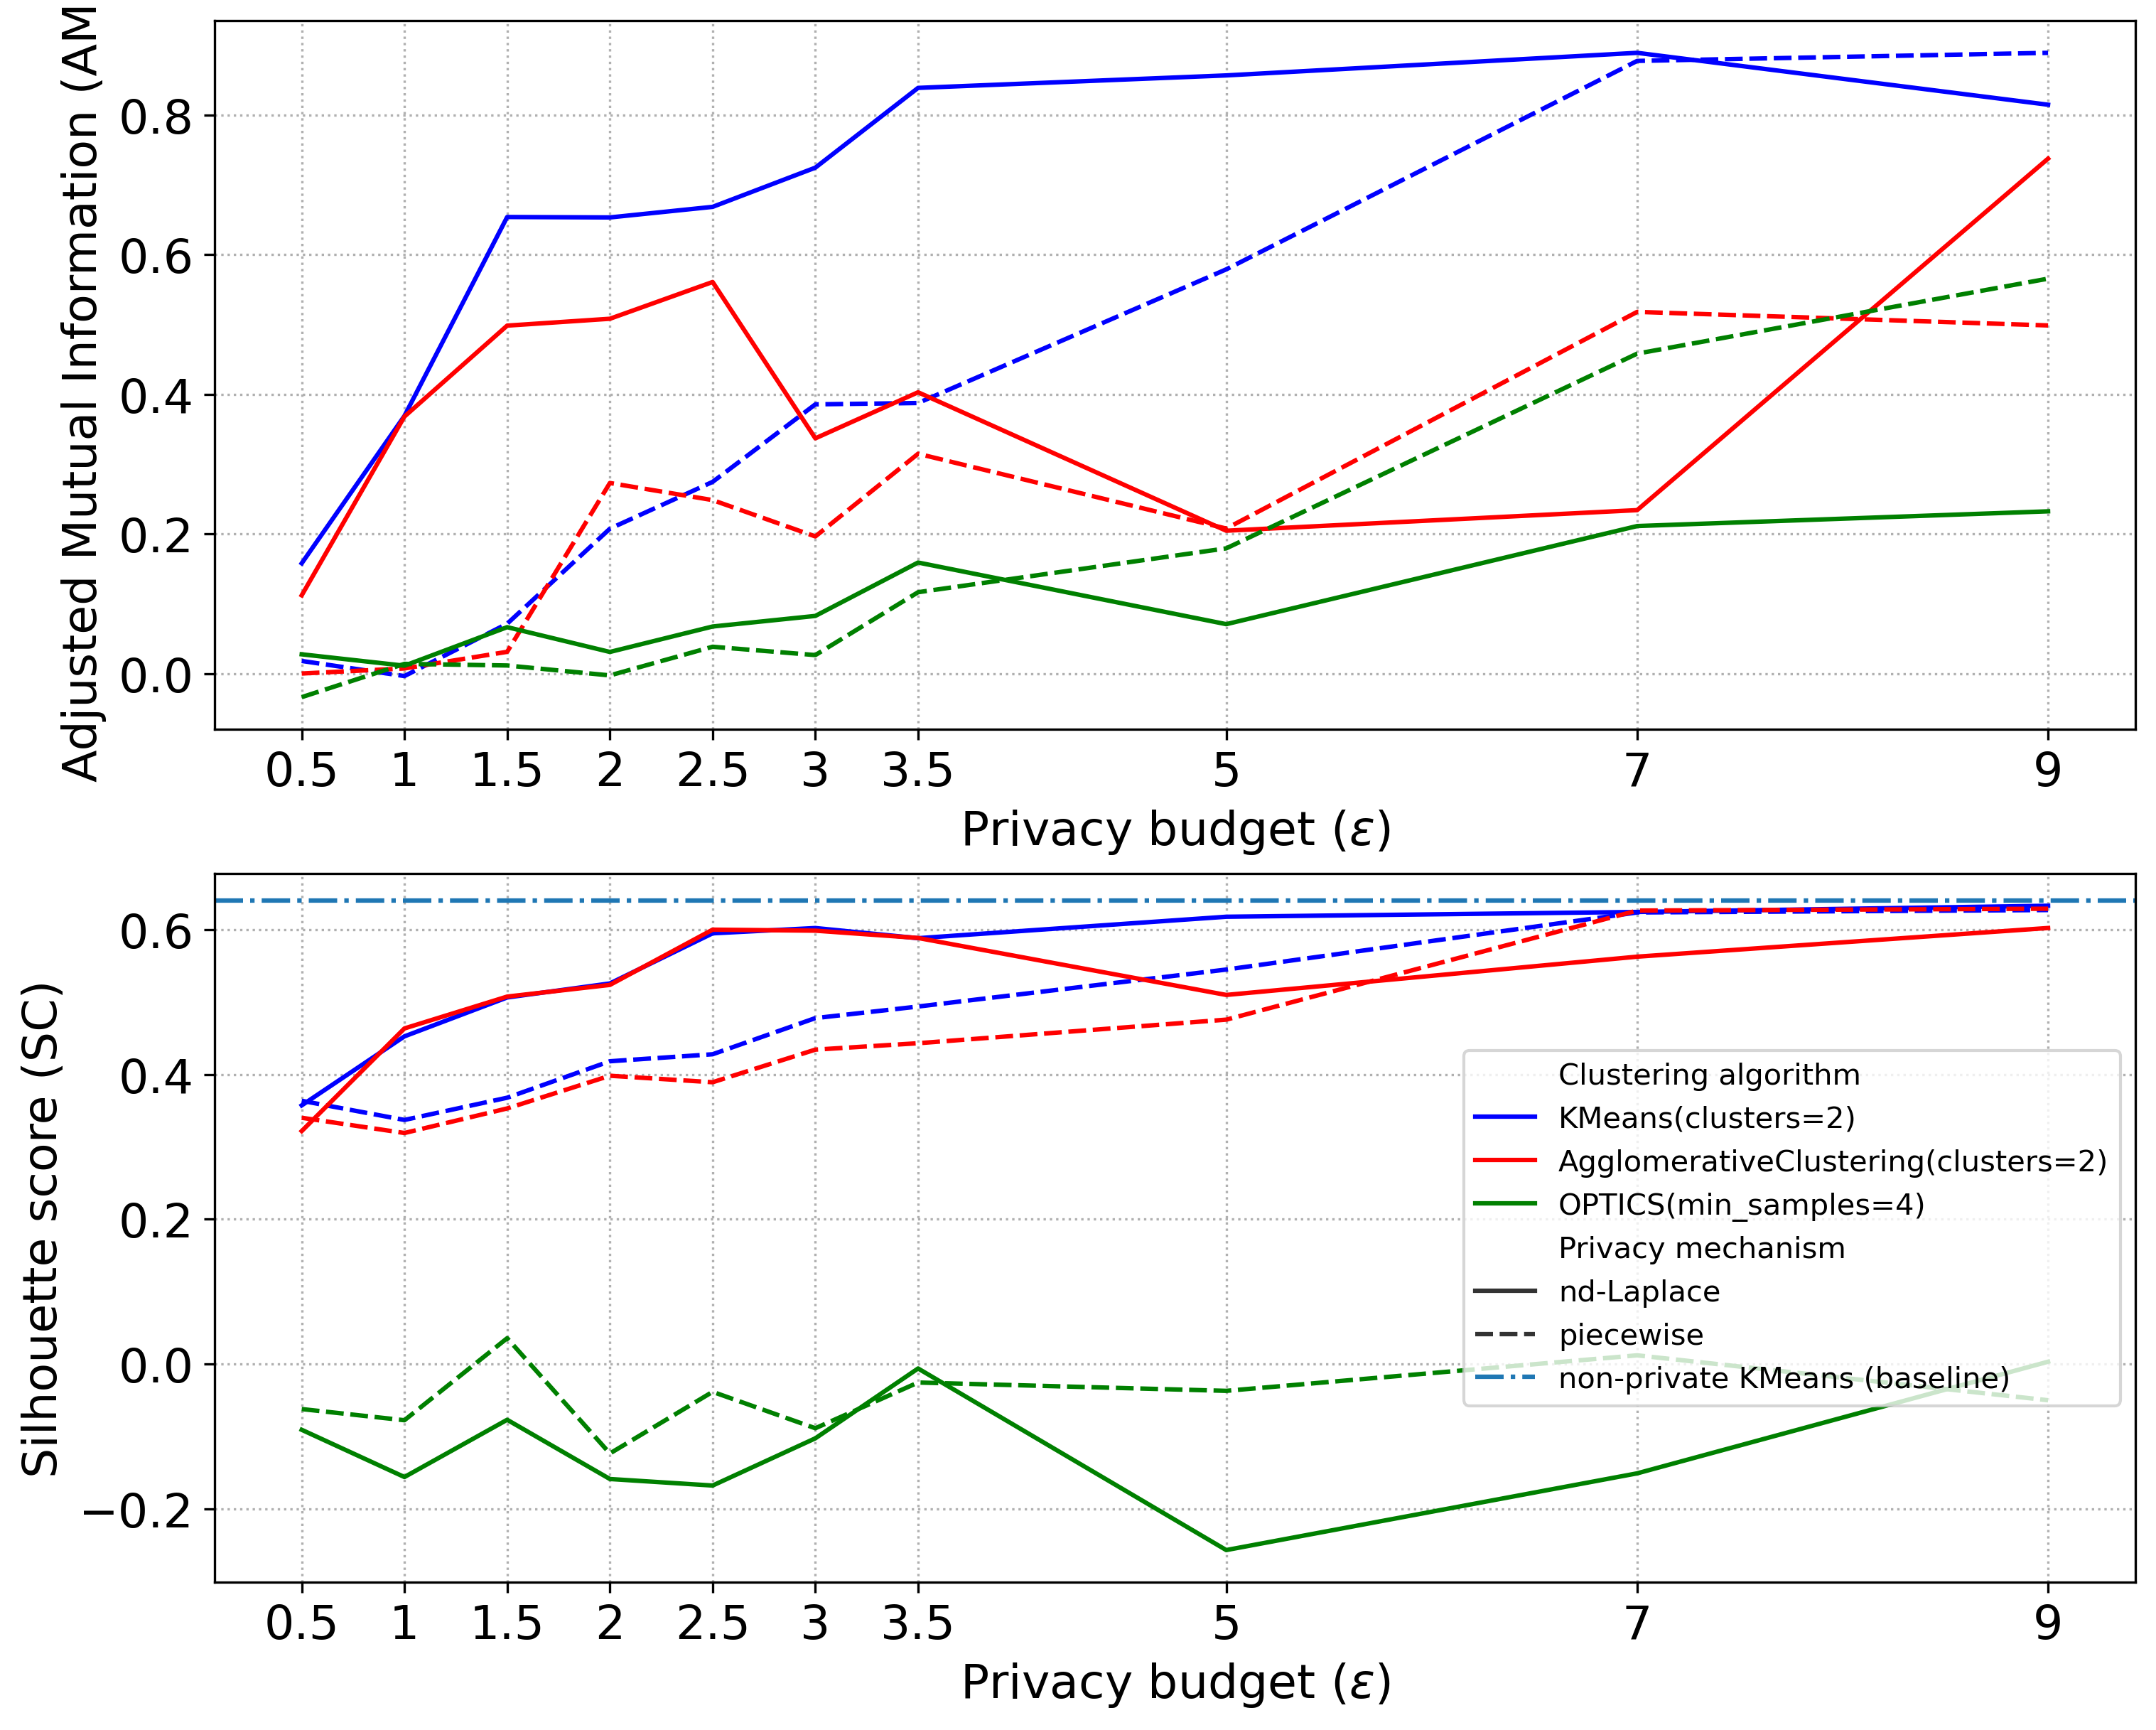
\includegraphics[width=1\textwidth]{Results/nd-laplace/nd-Laplace/seeds-dataset/ami-and-sc_2_dimensions.png}

  \label{fig:validation-seeds-dataset_comparison_2d-laplace}
\end{figure}
%The above plots show the AMI and ARI scores for the seeds-dataset with nD-Laplace/grid/optimal (left-side) and piecewise (right-side).
The Piecewise mechanism excels in Adjusted Mutual Information (\gls{ami}) at a privacy budget (epsilon) of 9, while the nD-Laplace mechanism is superior for other epsilon values. K-Means consistently outperforms other clustering algorithms, though only marginally over \gls{ag}, and both yield similar silhouette coefficient (\gls{sc}) scores. The under performance of the \gls{optics} algorithm across both mechanisms, suggest an incorrect configuration of this algorithm. The next page analyzes this behaviour.

The plot shows that nD-Laplace performs better for lower epsilons. Which is likely due to the mechanism also considering the shape (distance) of the data, so the Piecewise mechanism proportionally adds more noise. But, then we would expect \gls{optics} to score better. Therefore, we visualize this behaviour:
\begin{figure}[H]
  \centering
  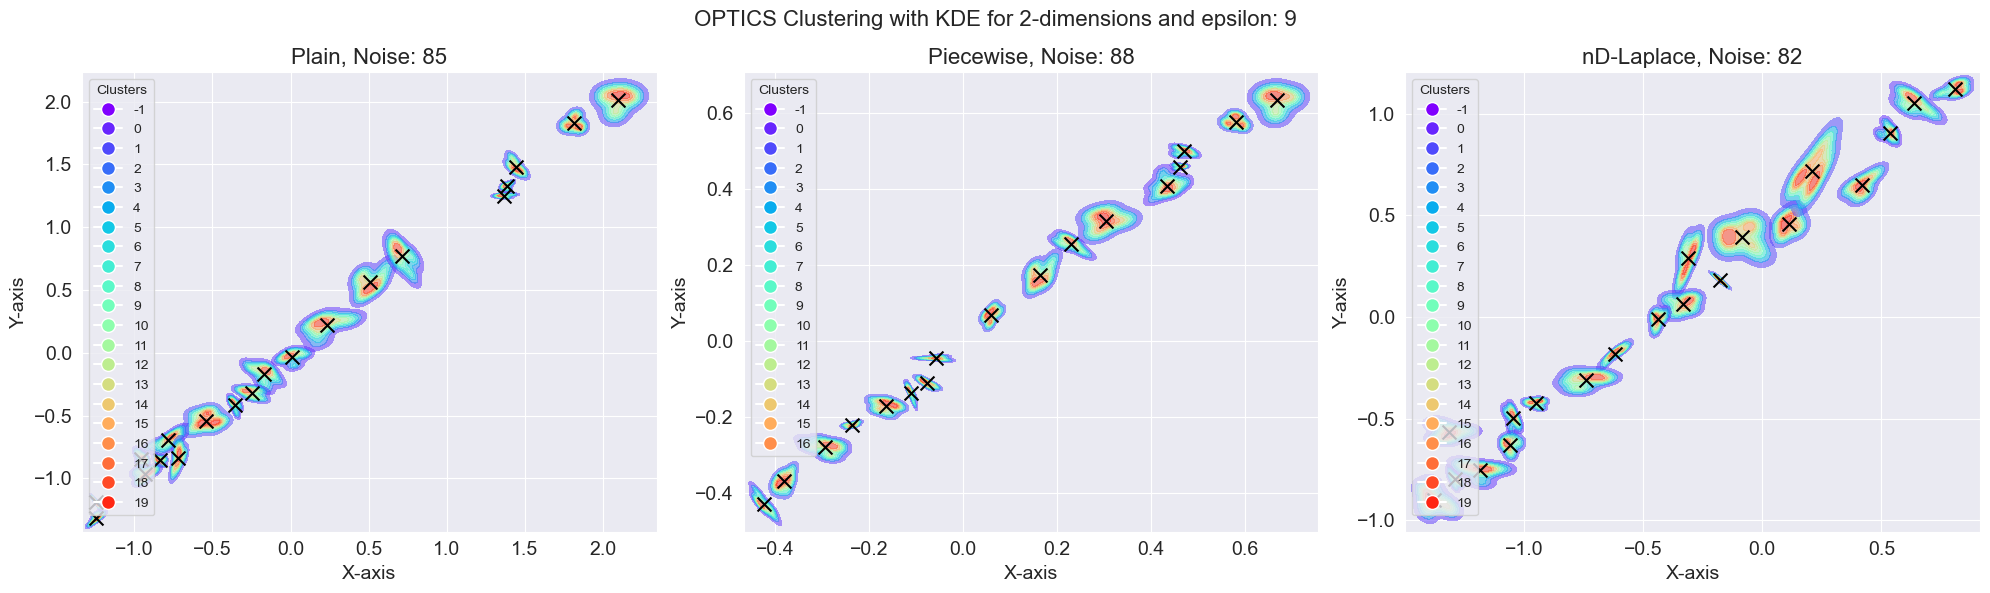
\includegraphics[width=1\linewidth]{Discussion/behaviour-2d-seeds-dataset&optics.png}
  \caption{Evaluating OPTICS for seeds-dataset 2-dimensional data (epsilon 9)}
  \label{fig:evaluate-optics-seeds-dataset-2d-9eps}
\end{figure}
The plot above illustrates the kernel density of core points chosen by the \gls{optics} algorithm for data with an epsilon value of 9. Clusters within the Plain and Piecewise datasets are compact and exhibit linear alignment, suggesting a distinct data distribution or directional noise stemming from the Piecewise mechanism. Conversely, the nD-Laplace clusters are more scattered, indicating that its noise impacts data uniformly across all directions.

Furthermore, the noise level is concerning. According to Schubert et al., the noise should range between 1\% and 30\% \citep{schubert_dbscan_2017}. However, the \gls{optics} algorithm we employed indicates an average noise level of 40\%, pointing to a potential problem with the algorithm's implementation. 
This issue is unrelated to the radios $\Pi$ of \gls{dbscan}, as it is automatically calculated by \gls{optics}.
Another hyper-parameter is $minPts$, which was set using the formula $minPts = 2 \cdot d$, where $d$ is the number of dimensions \citep{schubert_dbscan_2017}.
Schubert et al. also recommends increasing the minimum $minPts$ to compensate for noisy datasets.
This step was not included in the experiments, and likely one of the primary causes why the noise level is so high.

However, when comparing the noise counts of the various mechanisms, there is little difference.
Nevertheless, $minPts$ also has a substantial impact on the number of clusters, which is especially sensitive to the uniform distribution of nD-Laplace.

%This parameter has specifically a big impact on the noise, as this value is the distance threshold \citep{schubert_dbscan_2017}.
%Given that the noise count is very high, it is very likely the configuration is not correct or not suited for the distance function we use.
%This thesis constraints to the usage of Euclidean distance, but \gls{optics} can also be utilized using other distance calculations.
%Which means the threshold is differently interpreted.
%Therefore, it is likely a combination of $minPts$ and the distance function decisions have a big impact on the amount of noise.}
%This is also suggested by 

\newpage
\begin{figure}[H]
  \centering
  \caption{\textbf{AMI (top) and SC (bottom) for the nD-Laplace mechanism for the 2-dimensional data heart-dataset}}
  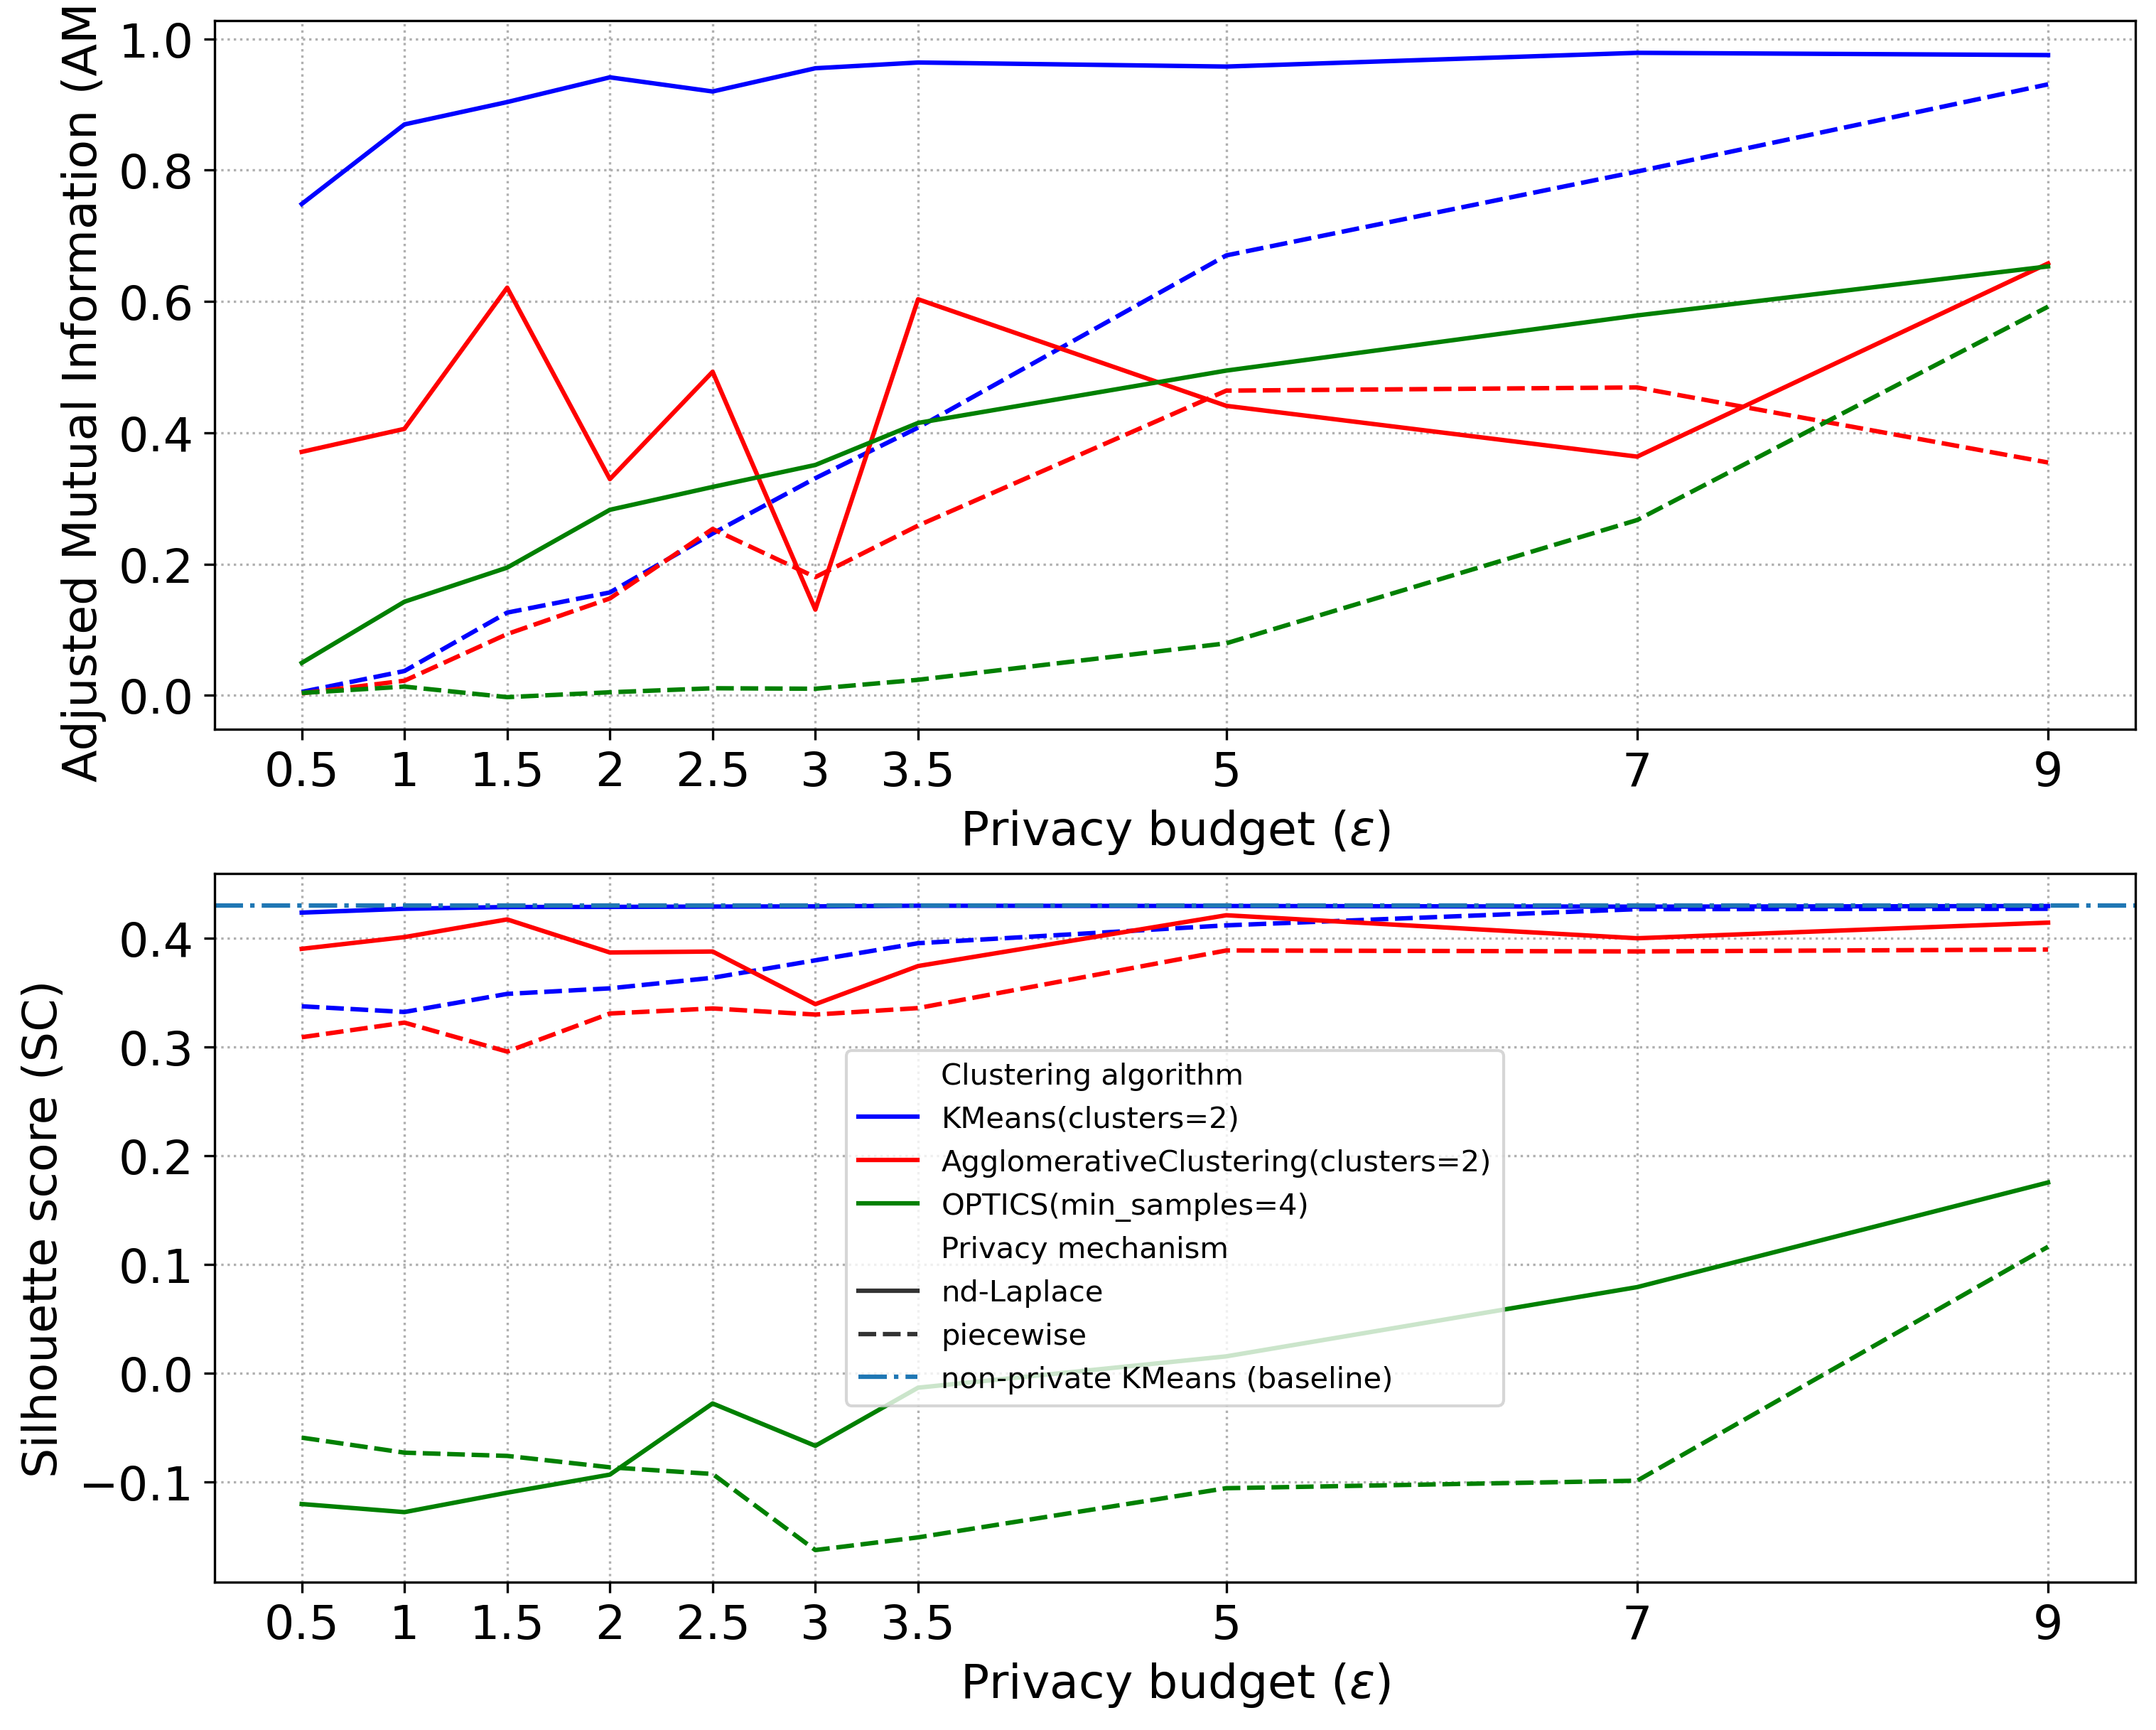
\includegraphics[width=1\textwidth]{Results/nd-laplace/nd-Laplace/heart-dataset/ami-and-sc_2_dimensions.png}

  \label{fig:validation-heart-dataset_comparison_2d-laplace}
\end{figure}
The K-Means method works better with nD-Laplace for all epsilon values. For other methods, the results between the two privacy systems are mostly the same. But, nD-Laplace often does a bit better in \gls{ami} scores. If we compare \gls{optics} with the previous section, we see large improvements.
When looking at \gls{sc}, both the grouped and K-Means methods do the best for both privacy systems. This is true for most methods. This \gls{ami} score trend matches what we saw with the \gls{optics} method earlier.

The trends observed in these charts closely mirror those from the seeds-dataset. However, the outcomes here are more consistent.
Remarkably, \gls{optics} stands out in its performance. This can be attributed to the data's configuration.
As depicted in Figure \ref{fig:evaluate-optics-seeds-dataset-2d-9eps}, there's a pronounced spread in the nD-Laplace data, similar to the heart-dataset.
When data is inherently well-separated, nD-Laplace excels, explaining the strong performance of both Agglomerative and K-Means clustering.
This observation is further supported by the \gls{sc}, which aligns closely with the baseline score of K-Means.
\newpage
\begin{figure}[H]
  \centering
  \caption{\textbf{AMI (top) and SC (bottom) for the nD-Laplace mechanism for the 2-dimensional data circle-dataset}}
  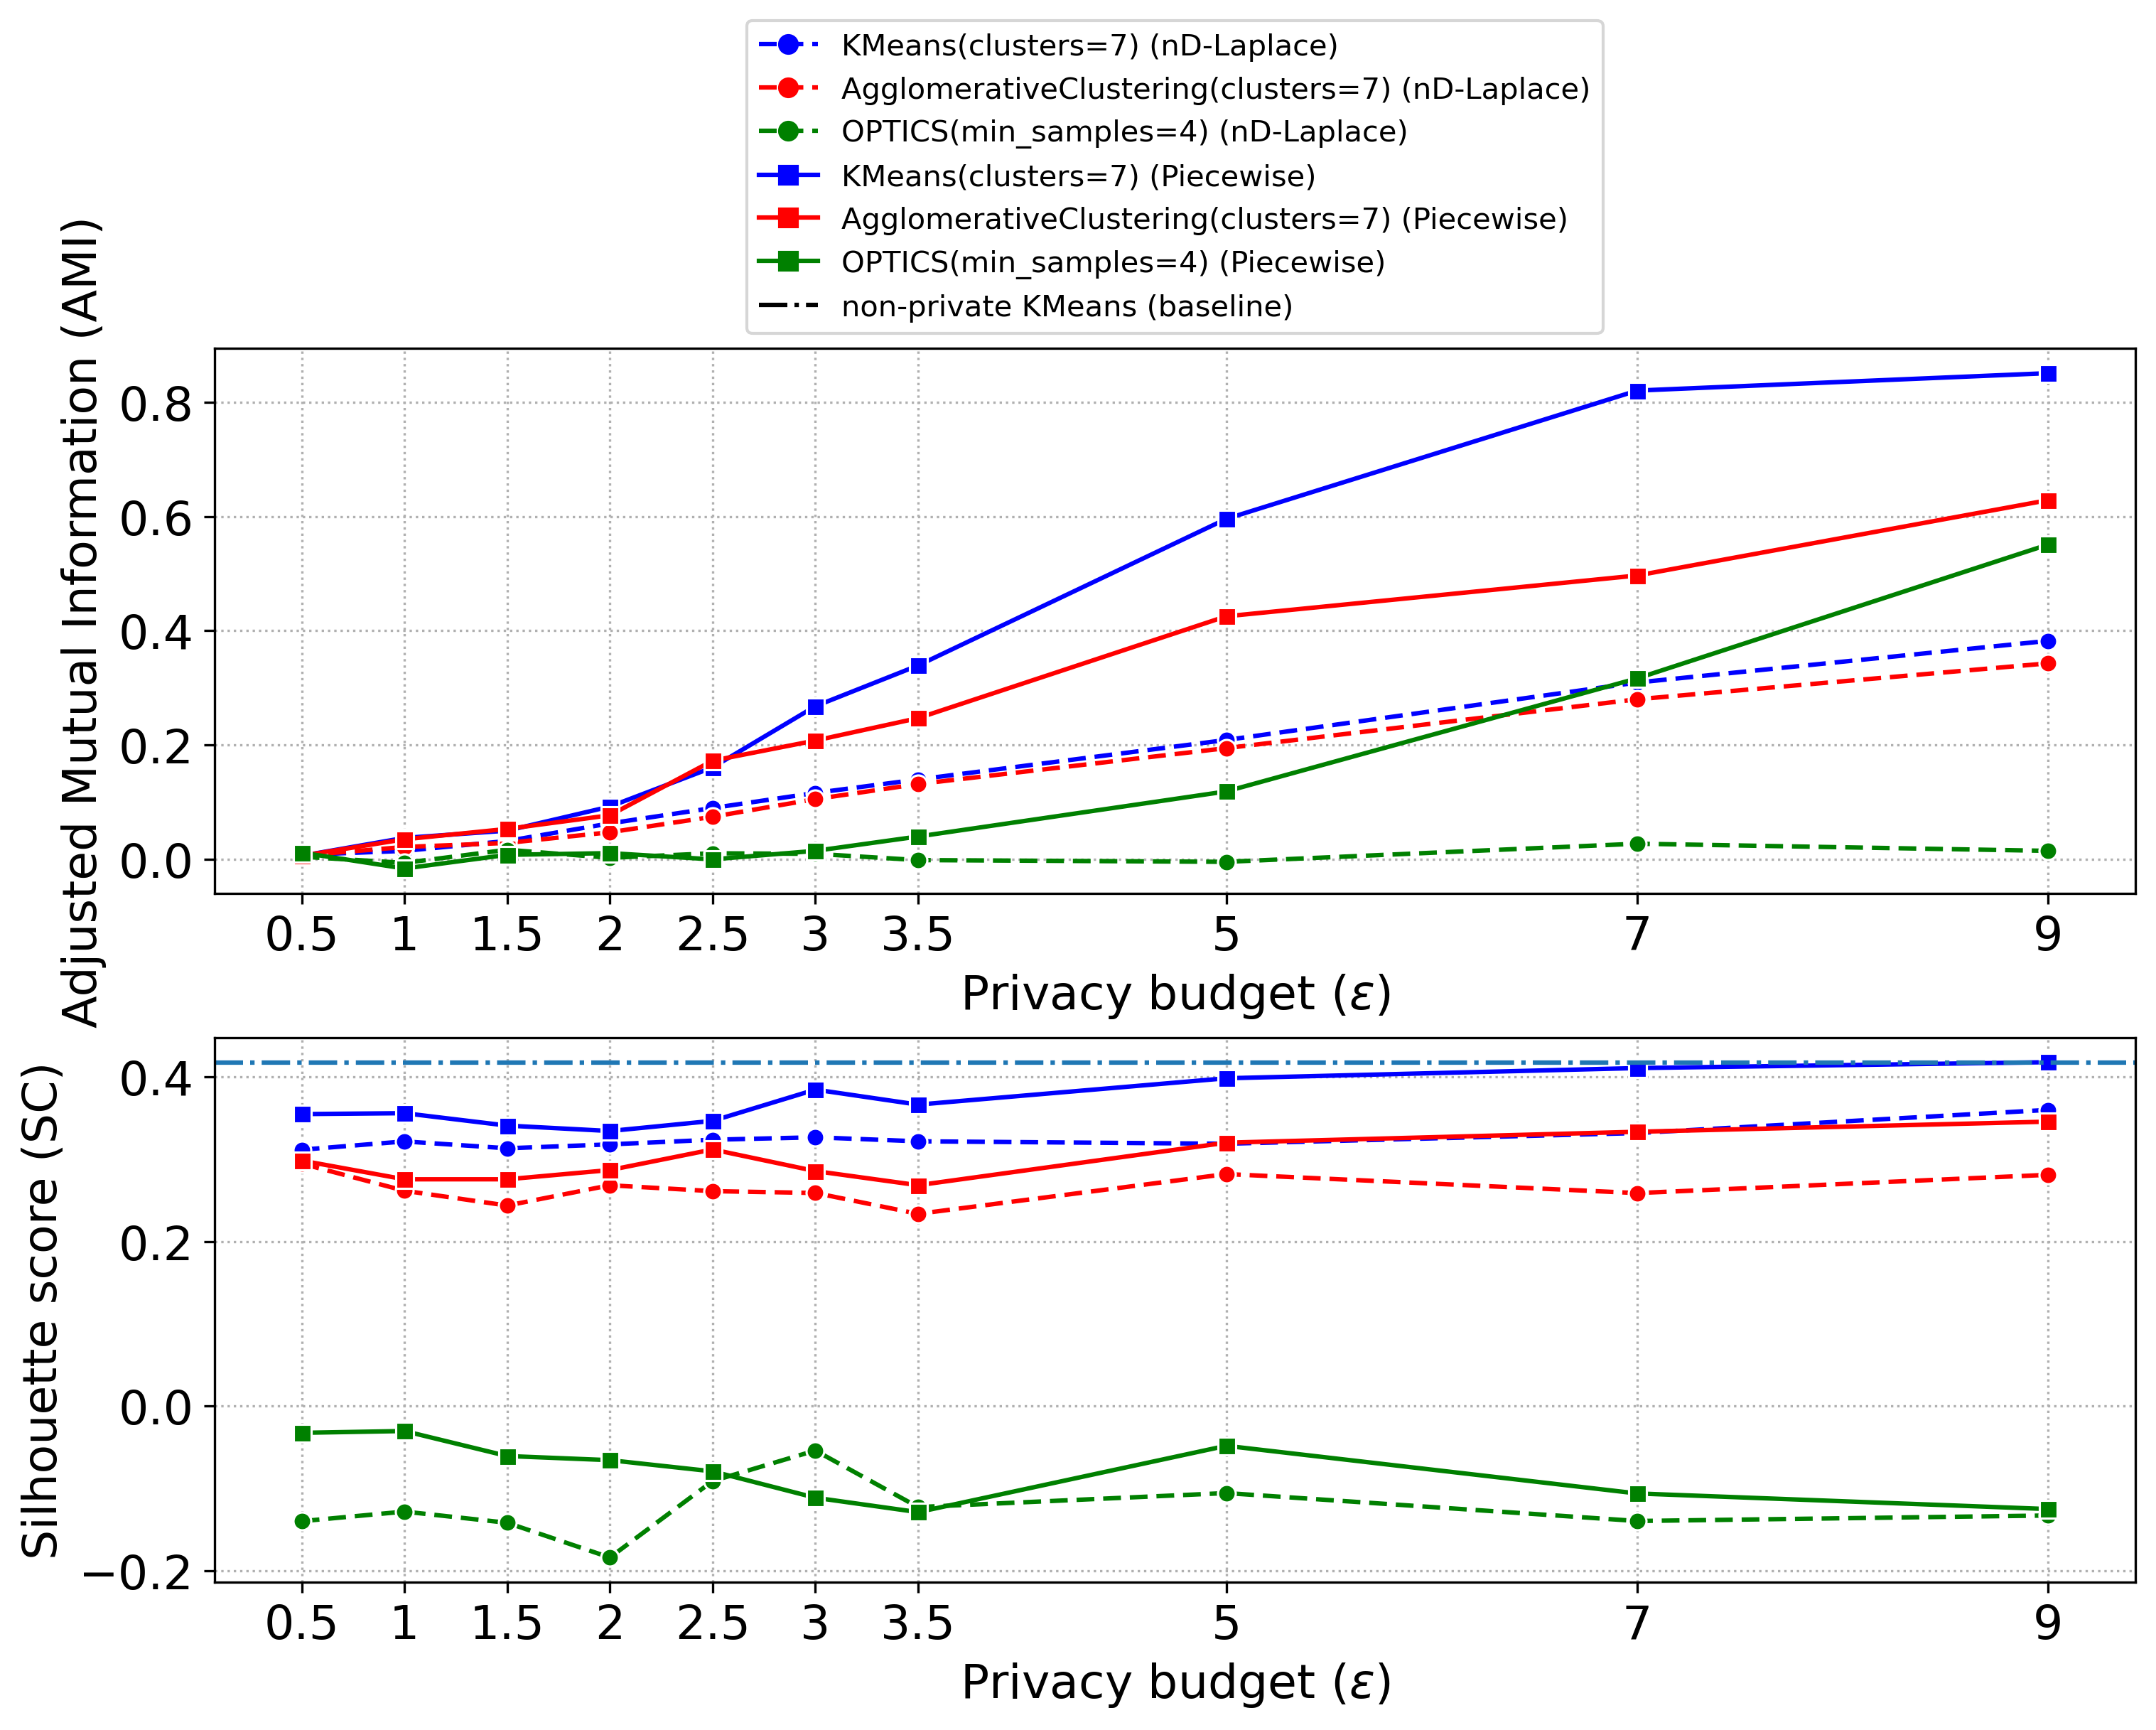
\includegraphics[width=1\textwidth]{Results/nd-laplace/nd-Laplace/circle-dataset/ami-and-sc_2_dimensions.png}
  \label{fig:validation-circle-dataset_comparison_2d-laplace}
\end{figure}
The Piecewise mechanism consistently achieves the highest scores for all \gls{ami} metrics. Analyzing the three algorithms, a recurring pattern emerges: K-Means leads in performance, trailed by Agglomerative and then \gls{optics}. Notably, within the nD-Laplace mechanism, \gls{optics} significantly lags behind the other algorithms. While a similar trend is observed in the \gls{sc} scores, the disparity between the two mechanisms is less pronounced. Yet, \gls{optics} consistently underperforms across all epsilon values.

We observe the same patterns as with the seeds-dataset; which is shaped as a line.
If there is a thiner line of data, the spread of the data is important. Piecewise mechanism handles this better, to stay close to the original line of data, while nD-Laplace's data is more spread. There are various factors why this issue impacts \gls{optics} the most, but this is probably due to the Euclidean space metric. Here, the distance matters more then similar metrics.
\newpage
\begin{figure}[H]
  \centering
  \caption{\textbf{AMI (top) and SC (bottom) for the nD-Laplace and Piecewise mechanisms for the 2-dimensional data line-dataset}}
  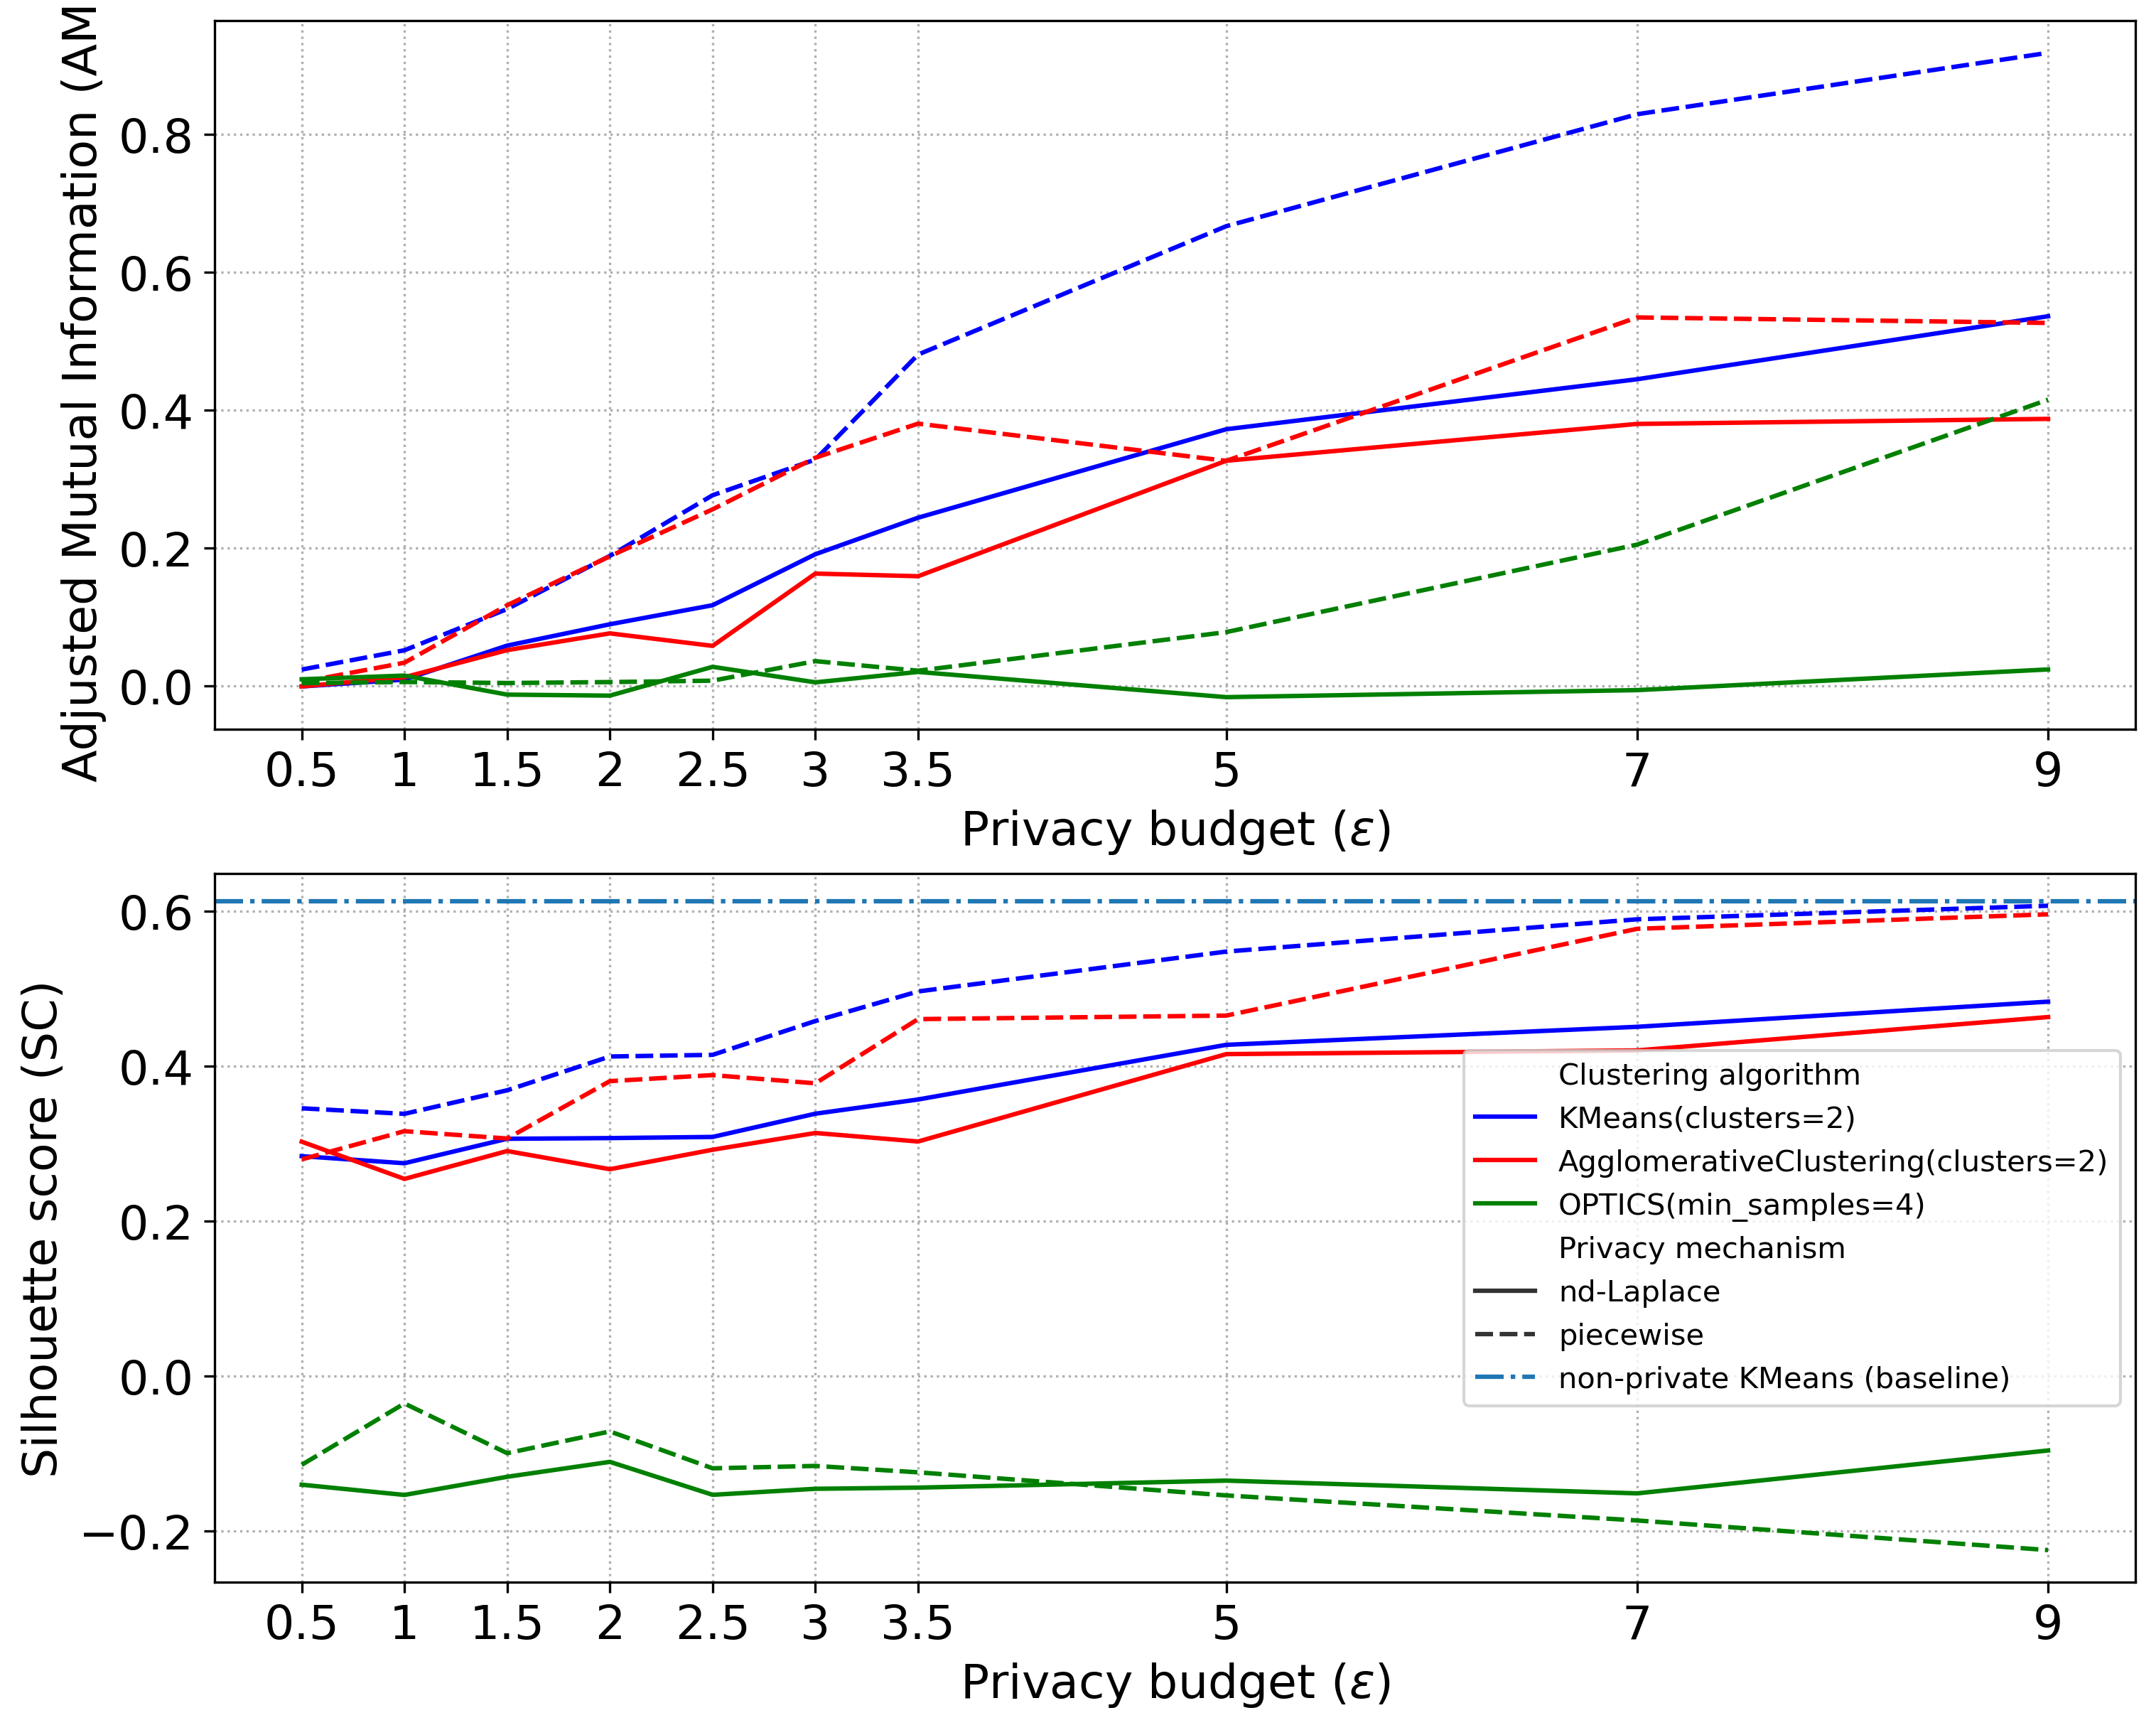
\includegraphics[width=1\textwidth]{Results/nd-laplace/nd-Laplace/line-dataset/ami-and-sc_2_dimensions.png}
  \label{fig:validation-line-dataset_comparison_2d-laplace}
\end{figure}
The nD-Laplace algorithm performs best with a privacy budget of 9 for K-Means (\gls{ami} 0.55 - 0.6).
\gls{ag} performs slightly worse with a budget of 9 (\gls{ami} 0.4).
Piecewise outperforms other methods, scoring 0.83 \gls{ami} for K-Means at budget 9 and better for different budgets, .
For \gls{sc}, the mechanisms have similar scores, with Piecewise at baseline from budget 5, nD-Laplace at 7, and \gls{ag} beyond baseline from budget 9.

Overall, the trends observed with the heart-dataset are not mirrored here. The Piecewise mechanism consistently outperforms nD-Laplace across nearly all privacy budgets. Given that the shapes of the line-dataset and seeds-dataset are expected to be analogous, we further illustrate this with the subsequent plot:

\begin{figure}[H]
  \centering
  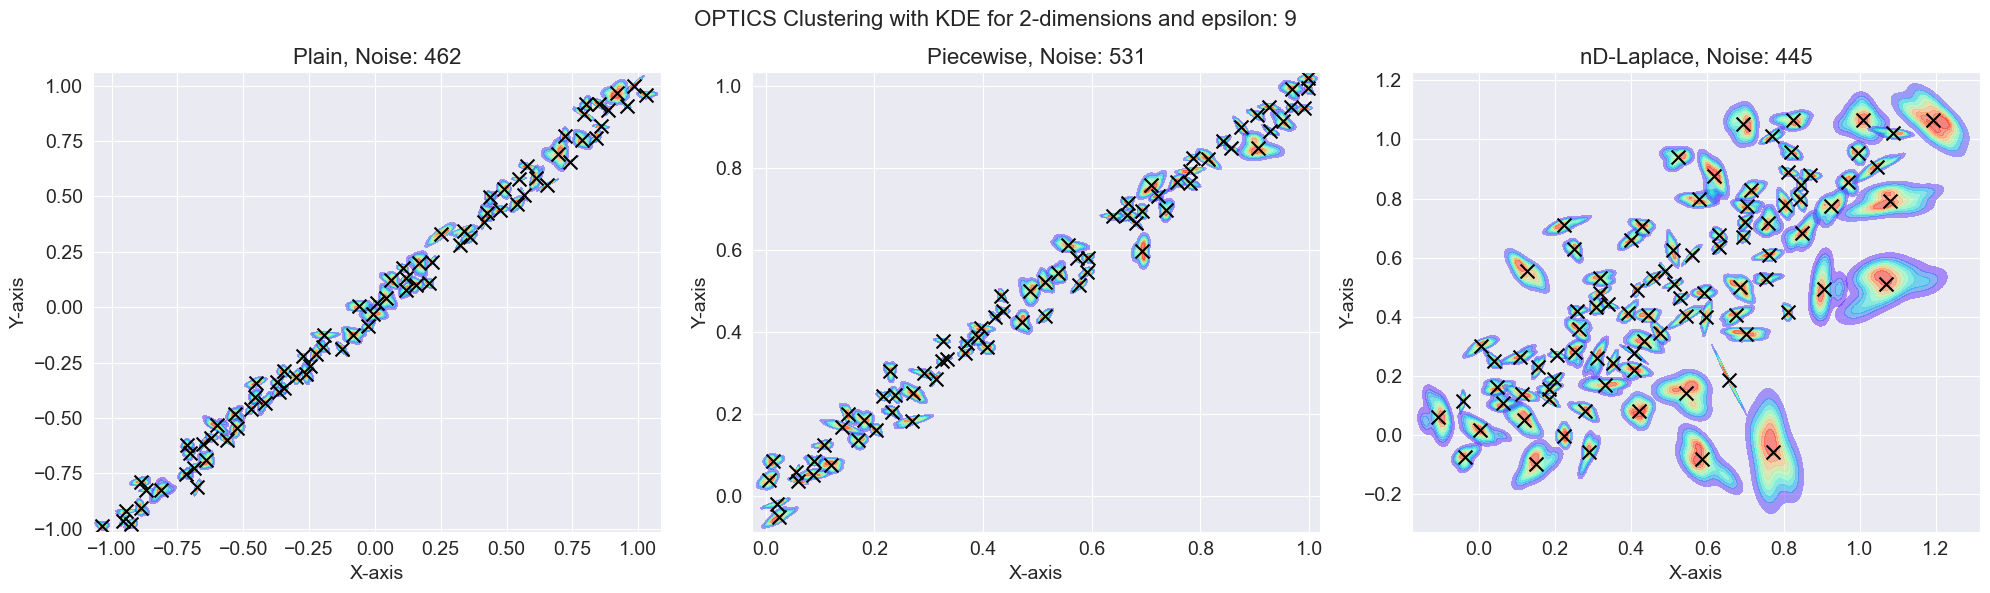
\includegraphics[width=1\linewidth]{Discussion/behaviour-2d-line-dataset&optics.png}
  \caption{Evaluating OPTICS and density of points for 2-dimensional Line dataset with epsilon 9}
  \label{fig:validation-Line-dataset_comparison_2d-laplace}
\end{figure}

The plot above displays the \gls{optics} scores, denoted by black markers. Even though the data bears resemblance to the seeds-dataset, the dispersion is significantly greater for the nD-Laplace mechanism. This can be attributed to the line shape of the data, as the nD-Laplace mechanism disperses noise uniformly in all directions. However, the extent of this dispersion is notably greater than that observed in the seeds-dataset, leading to inferior results.
The most probable reason for this is the amount of data-samples.
The likelihood to generate $z$ close to $x_0$ is higher. However, the line dataset is 5 times more data and the data is more dense.

\newpage
\begin{figure}[H]
  \centering
  \caption{\textbf{AMI (top) and SC (bottom) for the nD-Laplace and Piecewise mechanisms for the 2-dimensional data skewed-dataset}}
  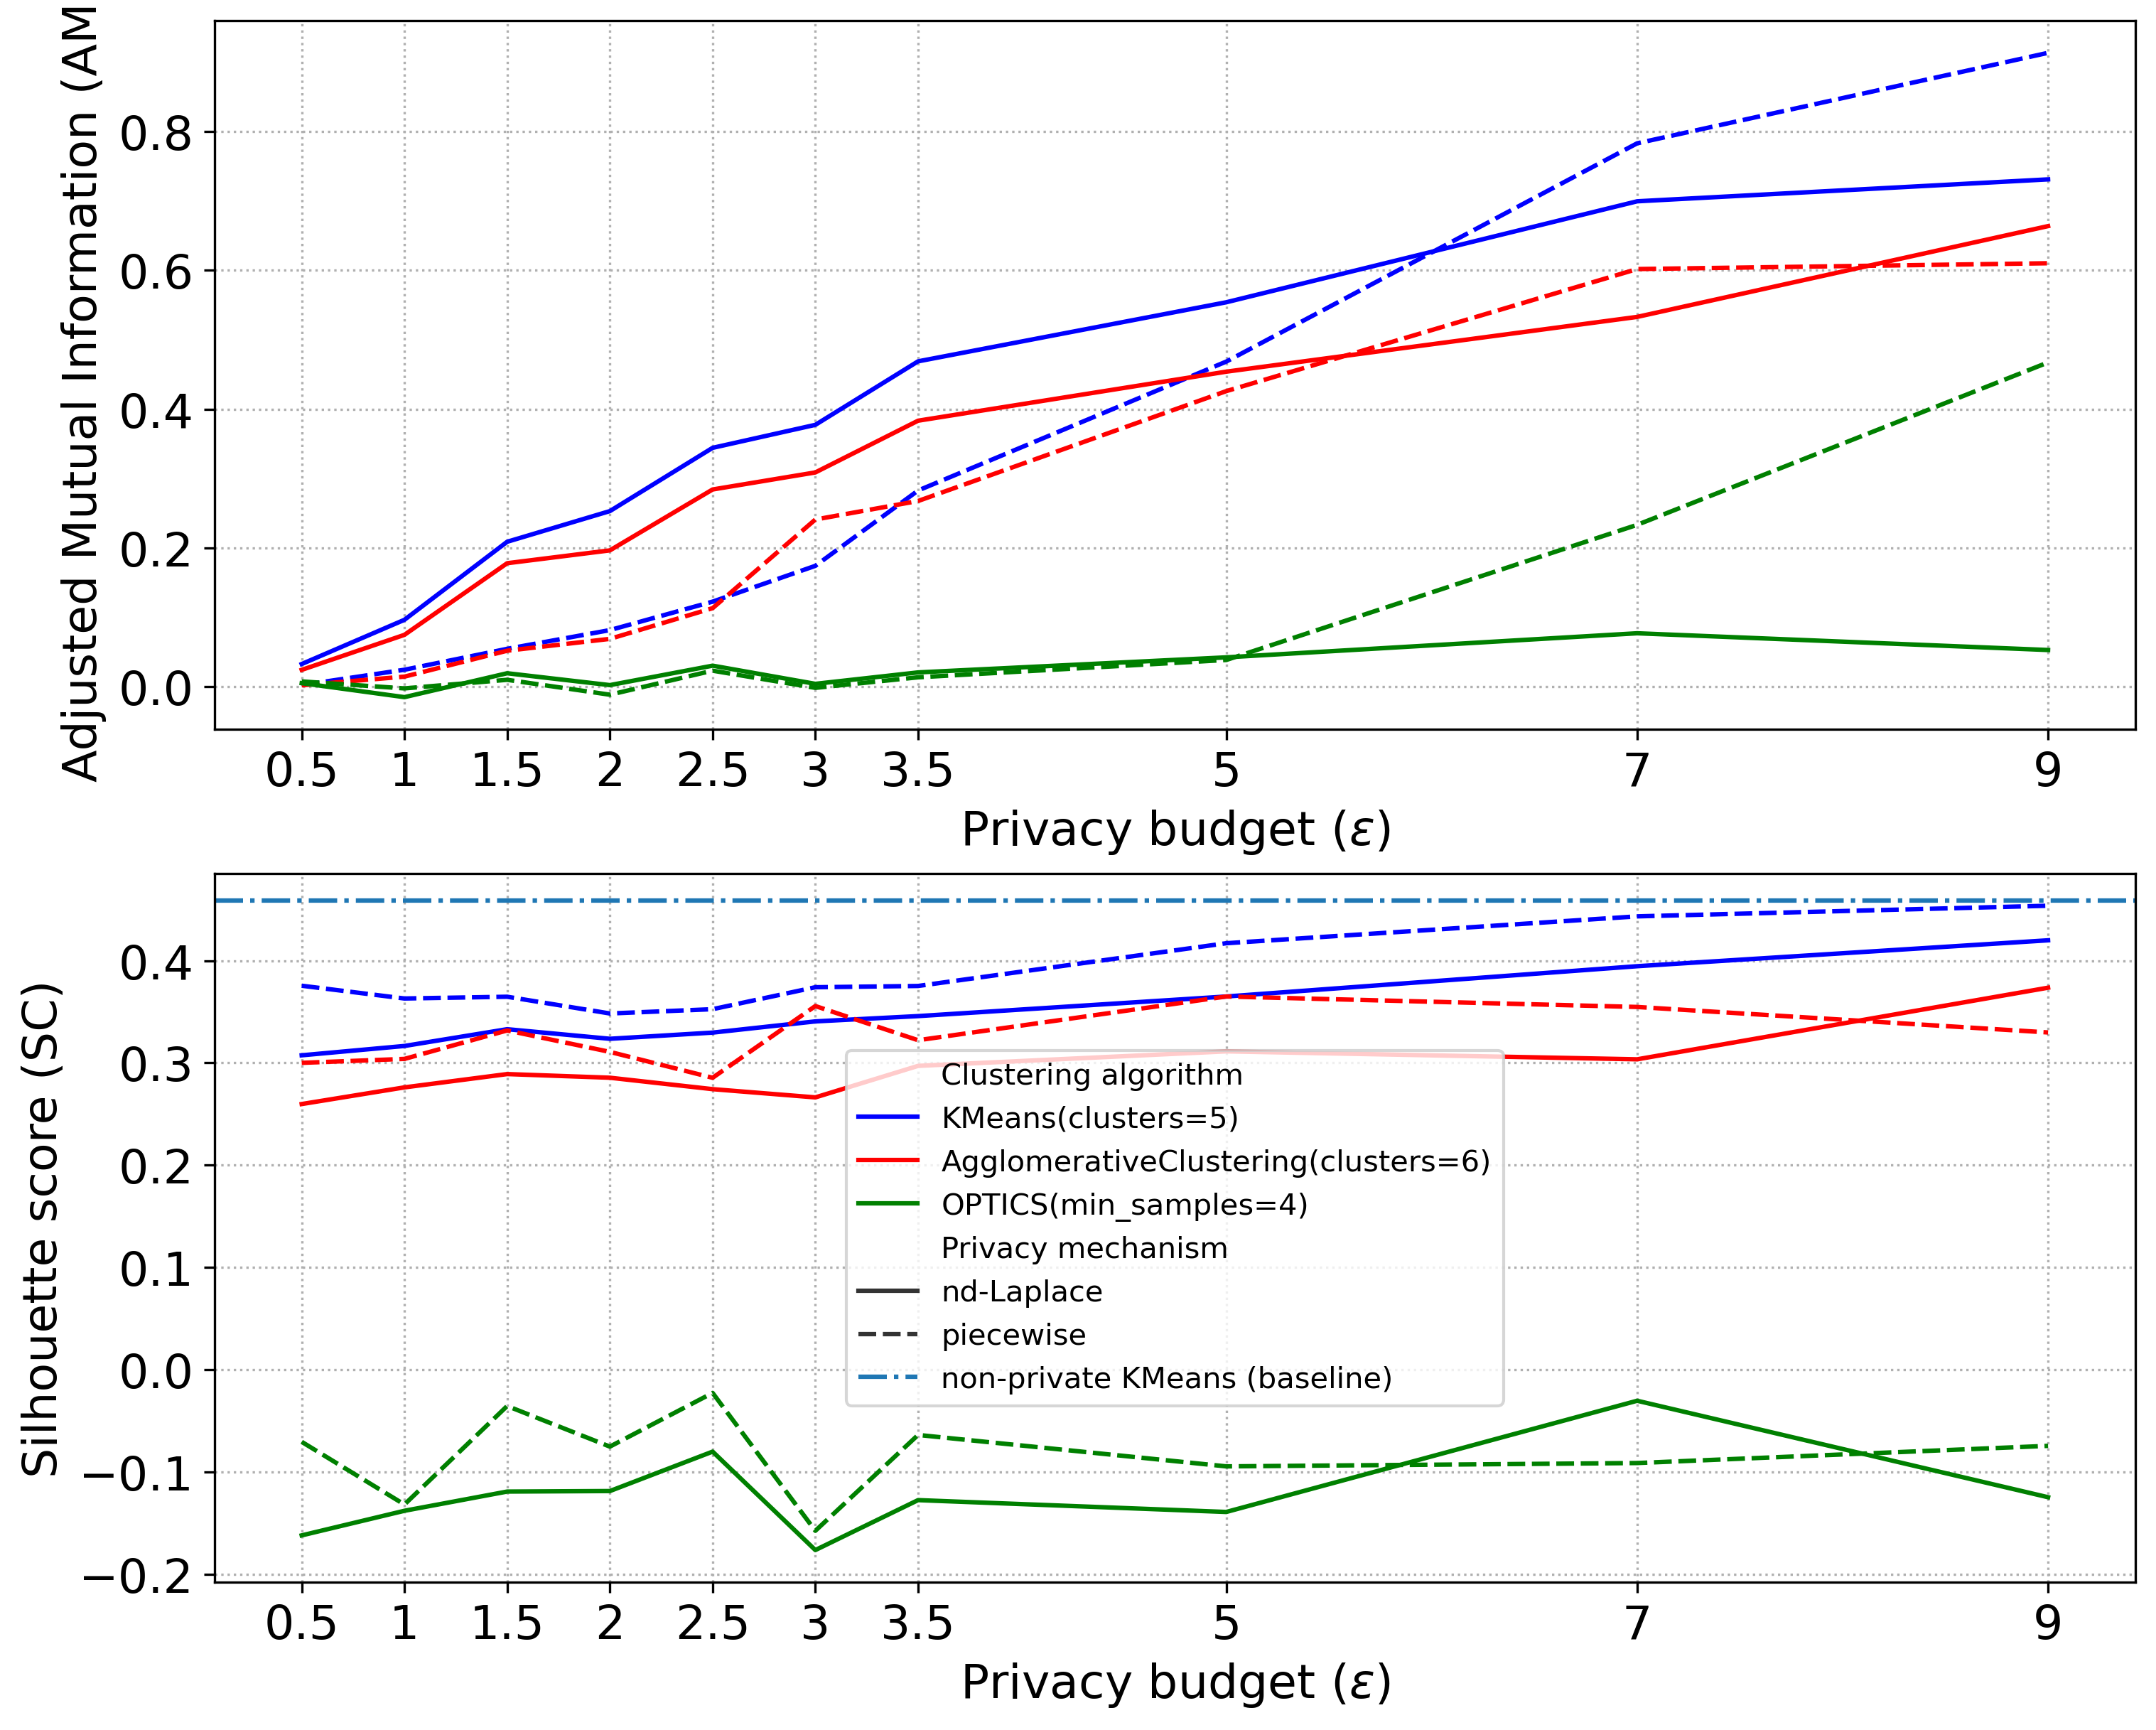
\includegraphics[width=1\textwidth]{Results/nd-laplace/nd-Laplace/skewed-dataset/ami-and-sc_2_dimensions.png}
  \label{fig:validation-skewed-dataset_comparison_2d-laplace}
\end{figure}
In our analysis, the nD-Laplace mechanism exhibits its peak performance when paired with K-Means, achieving an \gls{ami} range of 0.74 to 0.78 at privacy budgets of 7 and 9. Conversely, while Piecewise registers higher scores with K-Means for these specific budgets, it lags behind nD-Laplace for other privacy budgets. When considering the \gls{ag} scores, both mechanisms present comparable results. However, nD-Laplace has a slight edge, particularly at lower privacy budgets. This trend of nD-Laplace's superiority at reduced privacy budgets is consistent across different algorithms. A recurring observation is the under performance of \gls{optics}, although it still manages to score 0.43 at a privacy budget of 9 when using the Piecewise mechanism. As for the \gls{sc} metric, the patterns remain consistent: K-Means emerges as the top performer for both mechanisms, while \gls{optics} records notably low scores, even dipping below 0.0 for both mechanisms.

\newpage
\subsection{3-dimensional data}
\begin{figure}[H]
  \centering
  \caption{\textbf{AMI (top) and SC (bottom) for the nD-Laplace and Piecewse mechanisms for the 3-dimensional data seeds-dataset}}
  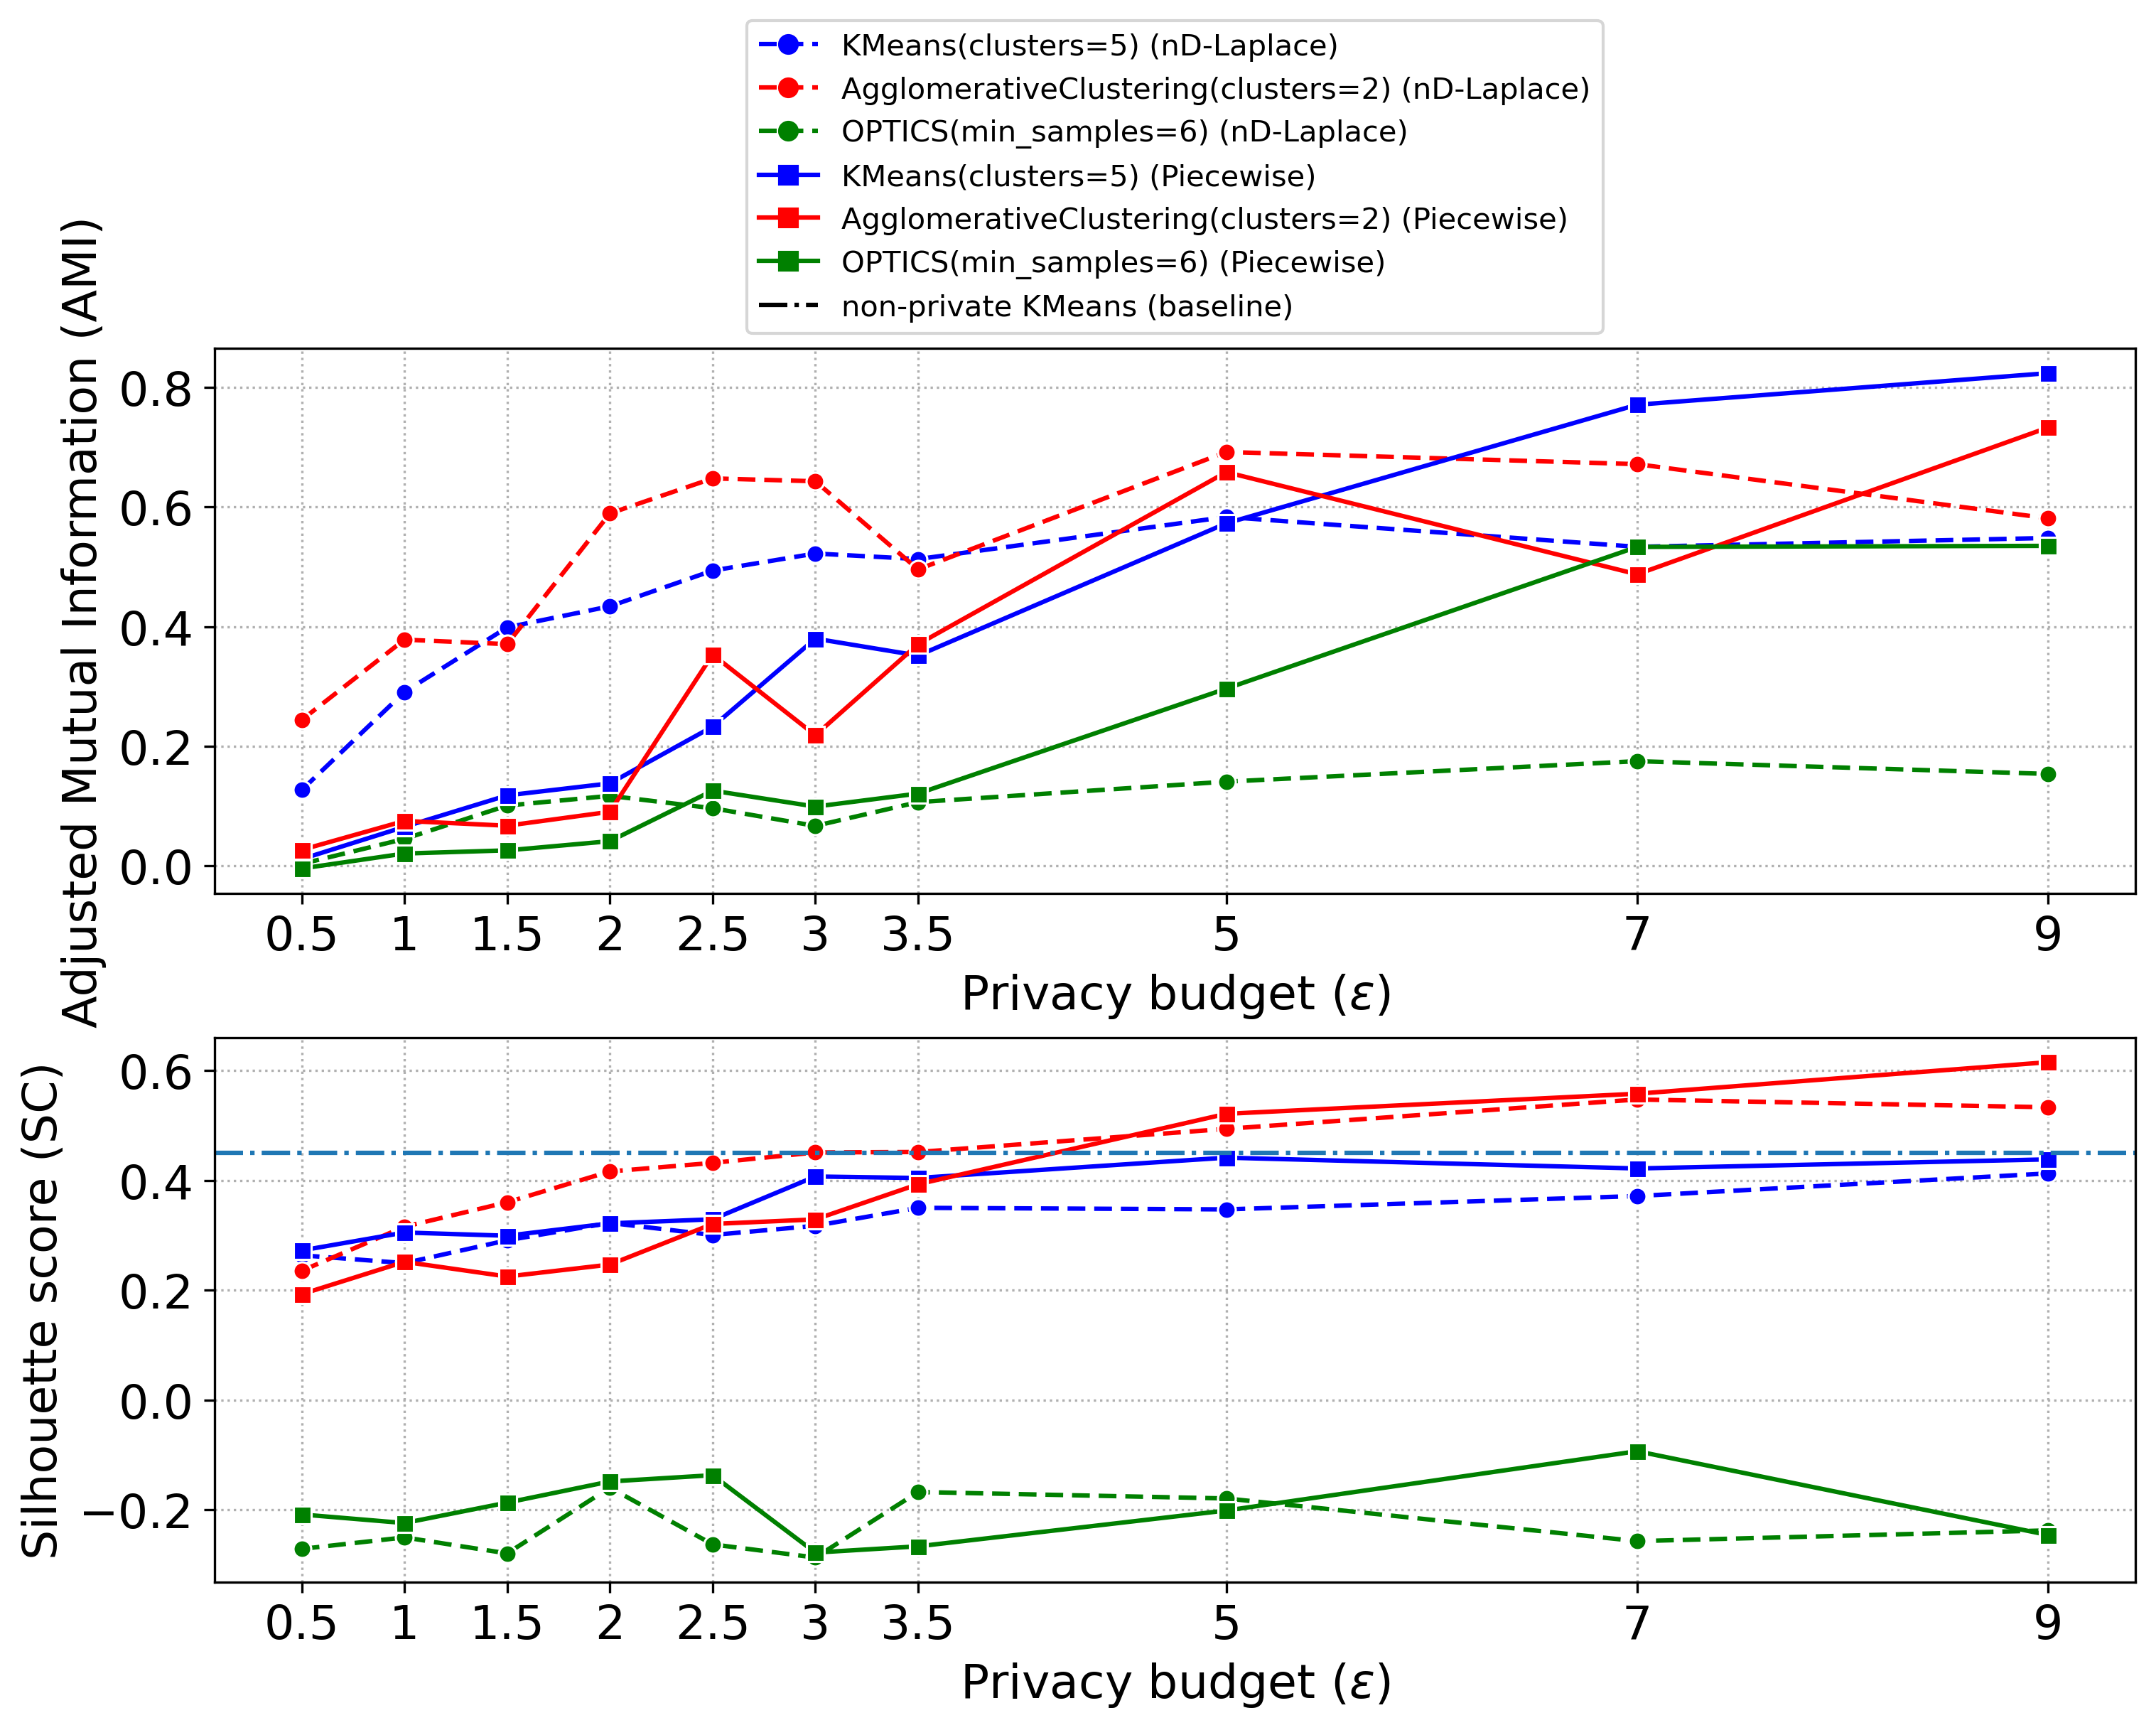
\includegraphics[width=1\textwidth]{Results/nd-laplace/nd-Laplace/seeds-dataset/ami-and-sc_3_dimensions.png}
  \label{fig:validation-seeds-dataset_comparison_3d-laplace}
\end{figure}
For the 3-dimensional data, the trend mirrors that observed in the 2-dimensional version of the seeds-dataset. In the range from 0.5 to 5, nD-Laplace outperforms both \gls{ag} and K-Means. Beyond this range, the Piecewise mechanism registers scores approximately 0.10 - 0.20 points higher than nD-Laplace. Conversely, nD-Laplace consistently scores higher for \gls{ag}, with the exception of epsilon 9. Notably, \gls{optics} yields a low score (less than 0.2 \gls{ami}) with nD-Laplace, whereas with Piecewise, the scores range between 0.2 and 0.58 for a privacy budget of 3.5.

For the \gls{sc} metric, the trend is consistent with the \gls{ami} score. However, \gls{ag} achieves a score surpassing the baseline for privacy budgets ranging from 3.5 to 9 across both mechanisms.

In other visual representations, both \gls{ami} and \gls{sc} metrics exhibit comparable trends. Yet, in this specific plot, \gls{ag} is superior to K-Means in performance. While the cluster quality is elevated, it does not translate to a higher \gls{ag} score. This suggests that while the mechanisms maintain clusters, they don't necessarily preserve the exact cluster configurations or sizes as observed with the non-private K-Means.

\newpage
\begin{figure}[H]
  \centering

  \caption{\textbf{AMI (top) and SC (bottom) for the nD-Laplace and Piecewise mechanisms for the 3-dimensional data heart-dataset}}
  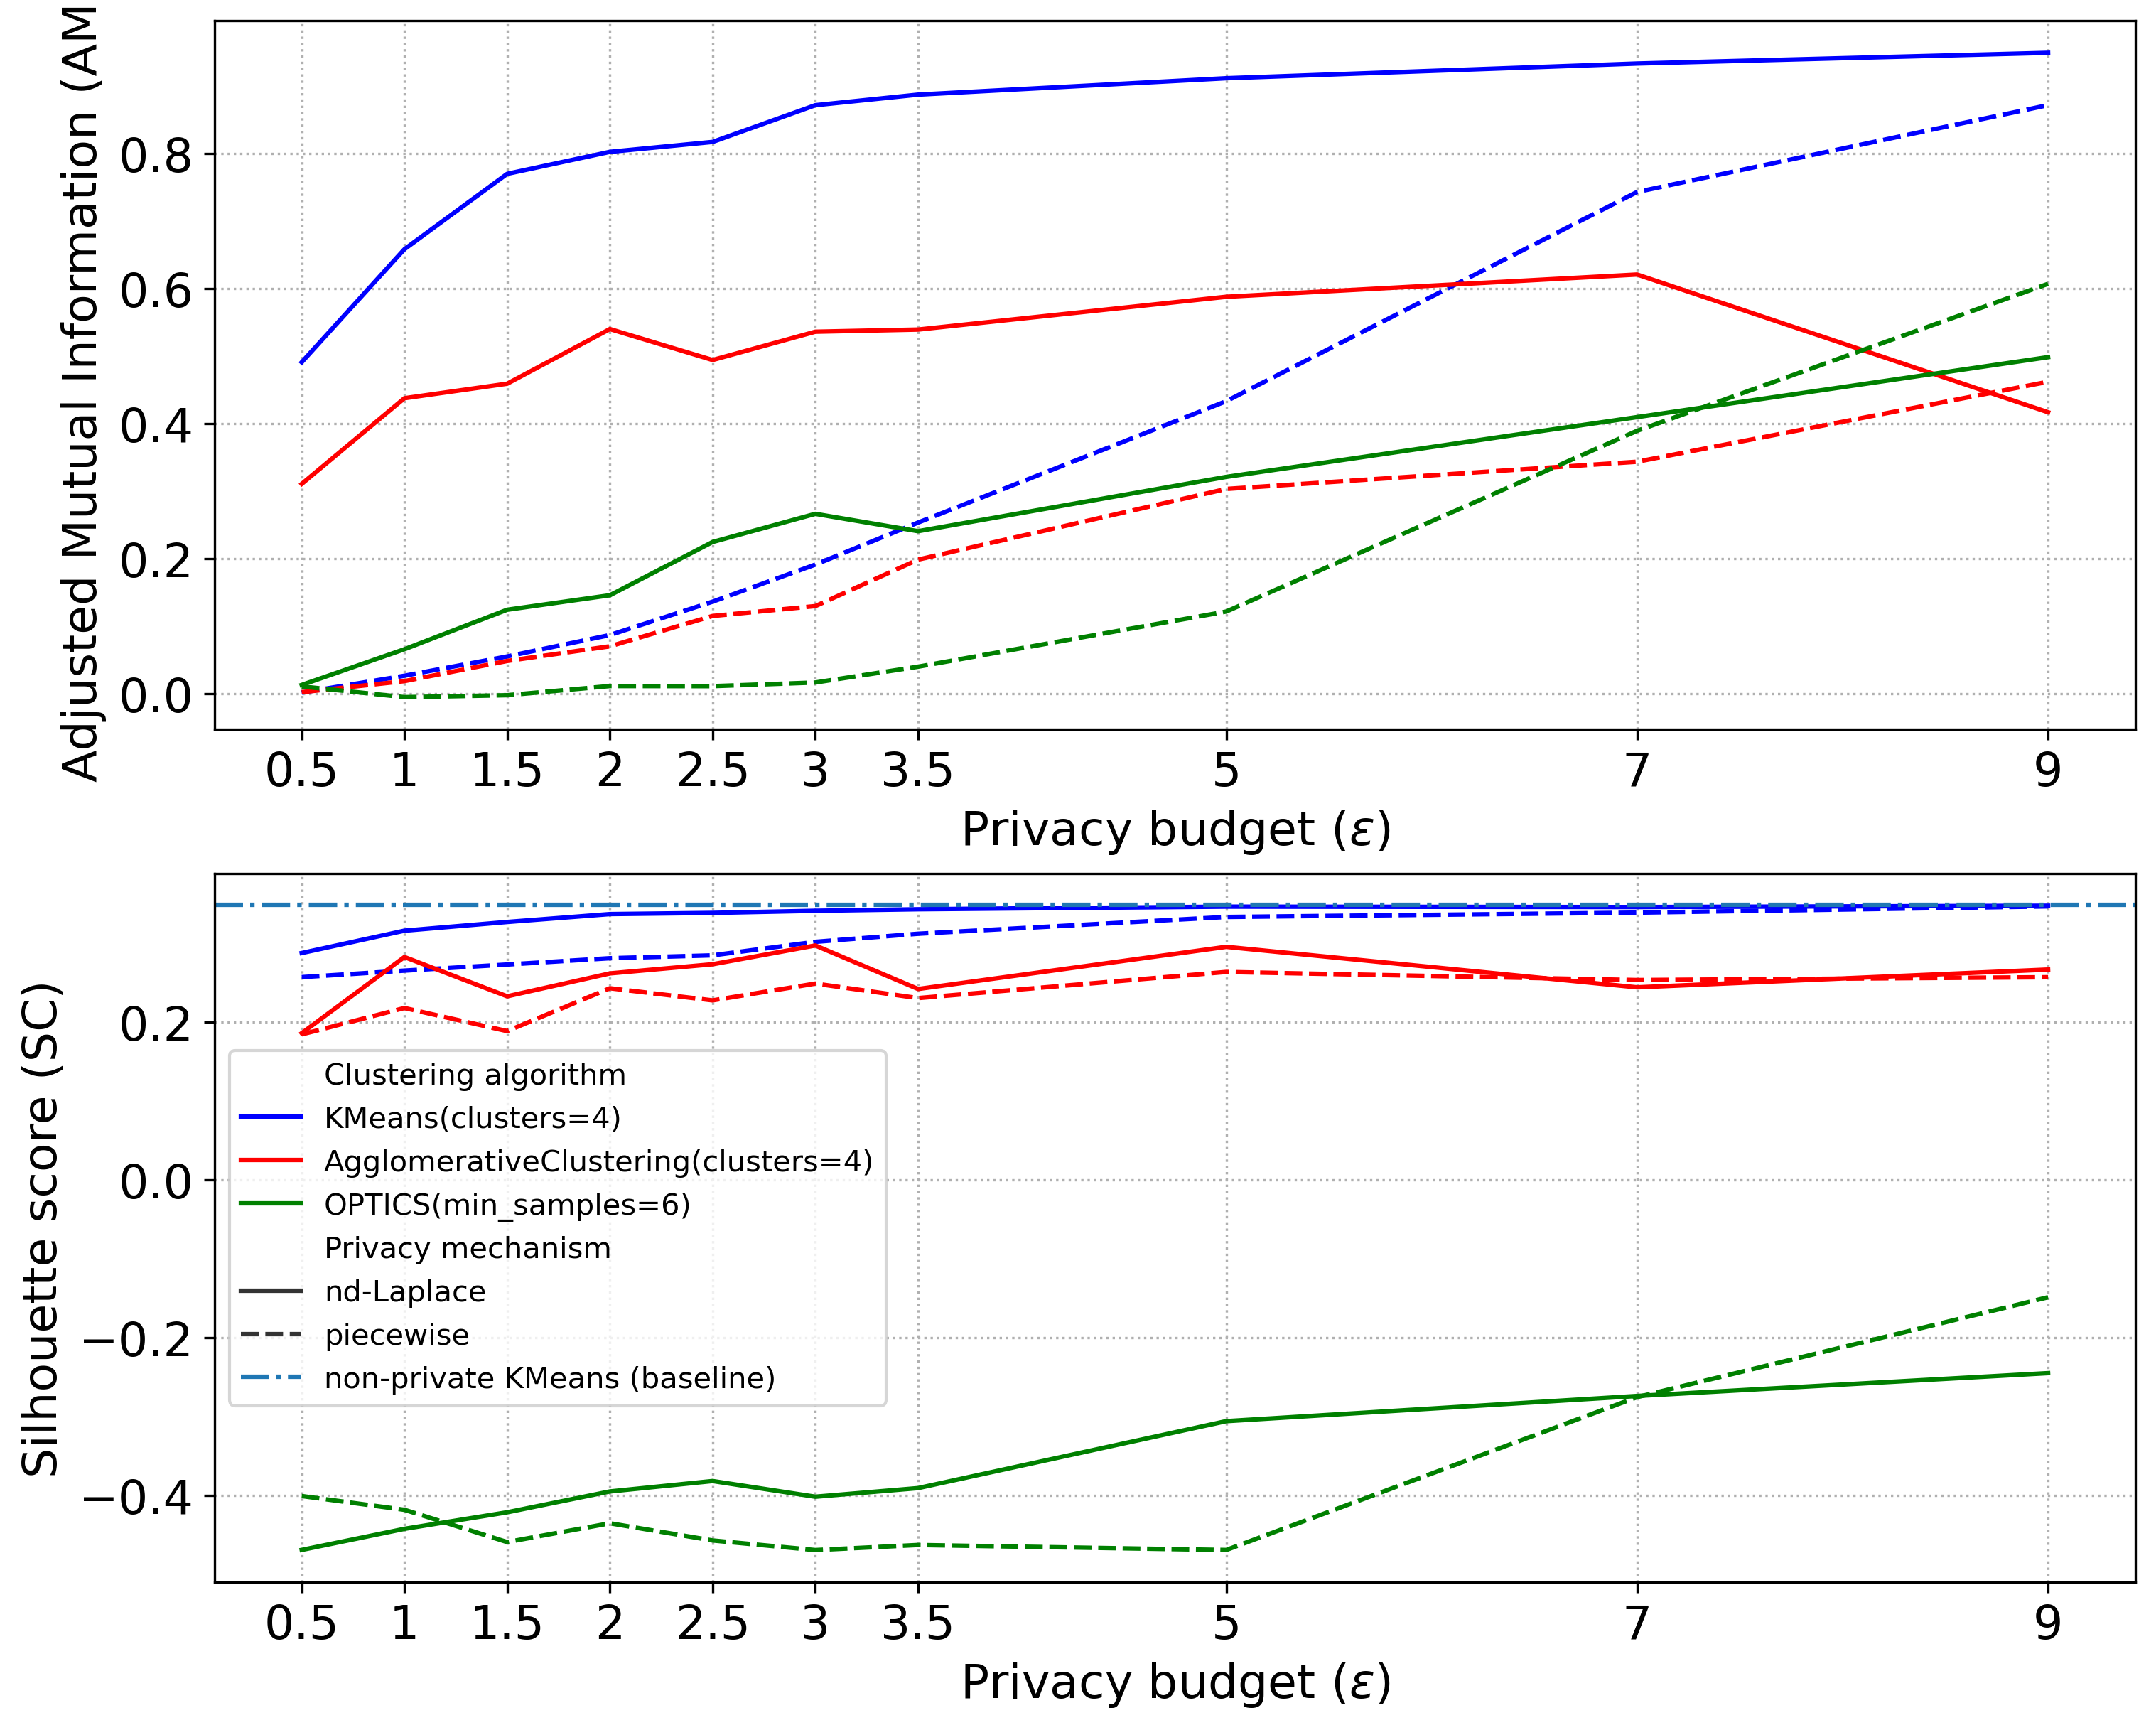
\includegraphics[width=1\textwidth]{Results/nd-laplace/nd-Laplace/heart-dataset/ami-and-sc_3_dimensions.png}
  \label{fig:validation-heart-dataset_comparison_3d-laplace}
\end{figure}
The nD-Laplace method gets good results, scoring around +/- 0.87 \gls{ami} for K-Means when the budgets are 7 and 9. This is similar to what we saw with the simpler 2D heart-dataset using the same method. We also noticed that \gls{optics} scores got better compared to other datasets, which matches the results from the 2D heart-dataset. However, \gls{ag} scores a bit lower than K-Means, but the overall pattern is similar.

For the Piecewise method, the scores are below 0.6 \gls{ami} when the budgets are less than 7, but it goes up to 0.8 \gls{ami} for K-Means. When we look at \gls{sc}, both Piecewise and nD-Laplace meet the standard scores for \gls{ag} and K-Means.

Even though \gls{optics} gets high scores for \gls{ami}, it does not do as well for \gls{sc}. The main job of \gls{ami} is to compare \gls{optics} to the non-private variant. But if \gls{sc} is low and \gls{ami} is high, it shows that also the non-private has incorrect clusterings.
\newpage
\begin{figure}[H]
  \centering

  \caption{\textbf{AMI (top) and SC (bottom) for the nD-Laplace and Piecewise mechanisms for the 3-dimensional data circle-dataset}}
  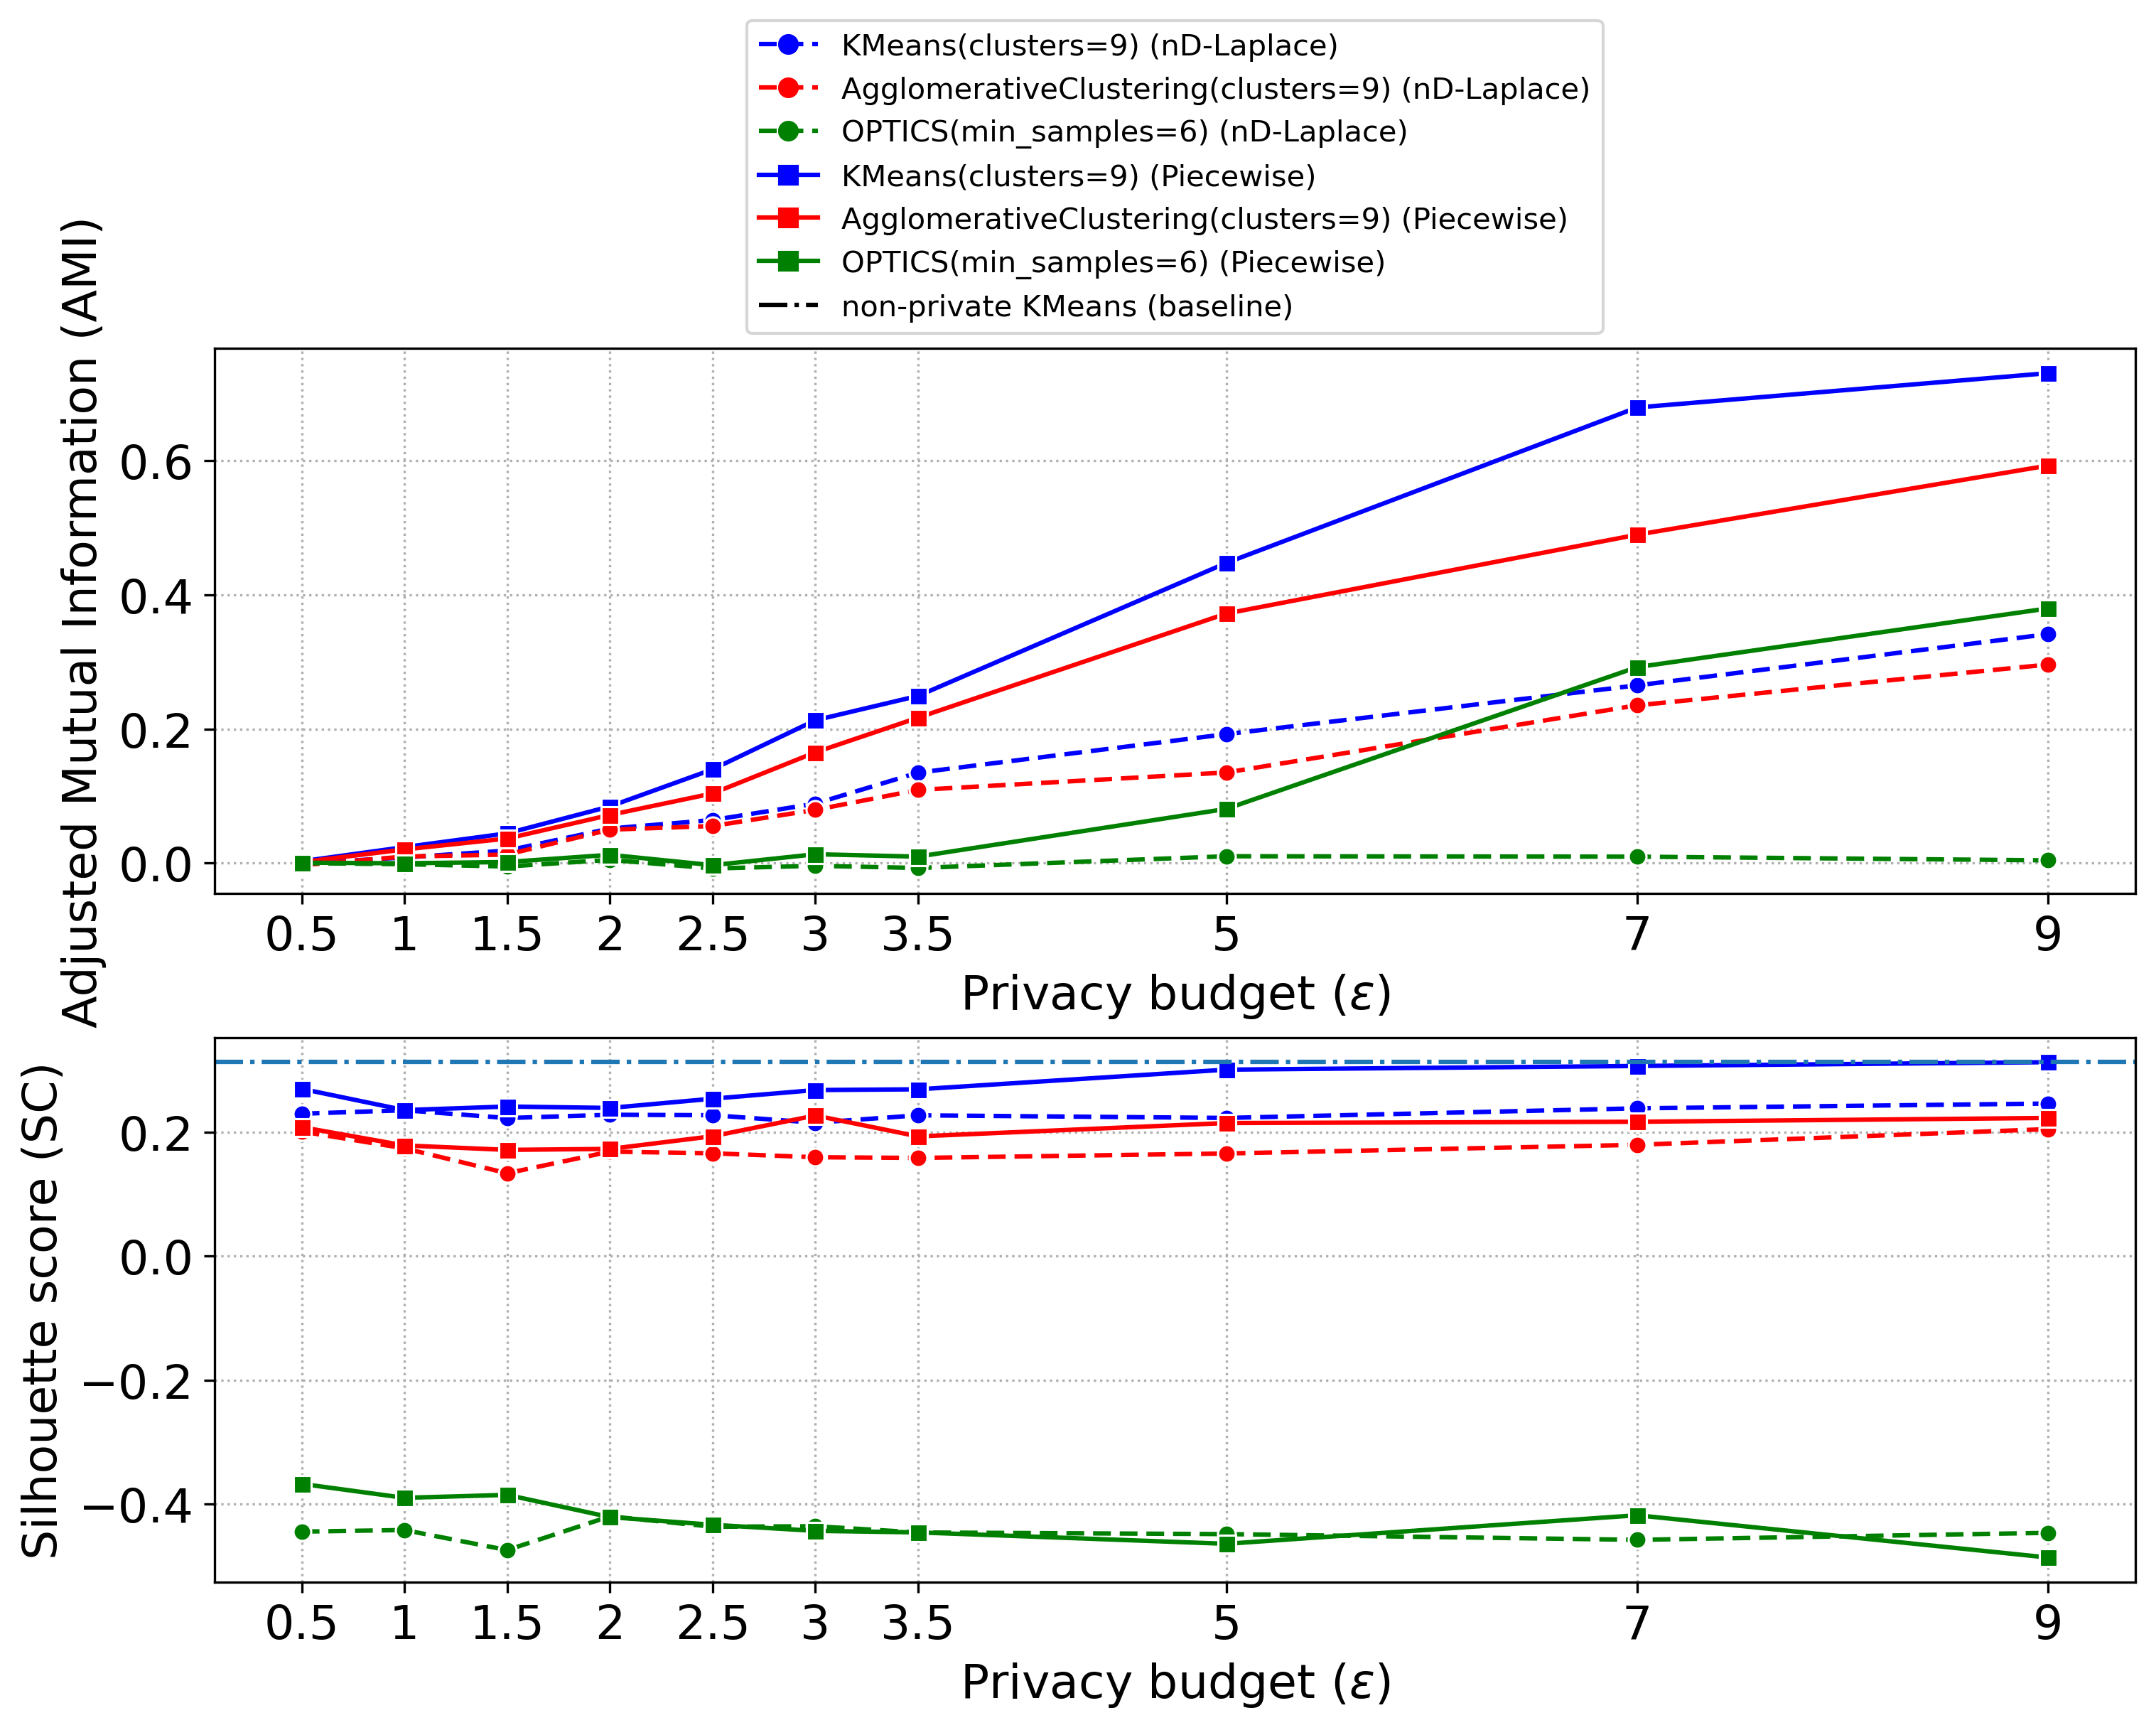
\includegraphics[width=1\textwidth]{Results/nd-laplace/nd-Laplace/circle-dataset/ami-and-sc_3_dimensions.png}

  \label{fig:validation-circle-dataset_comparison_3d-laplace}
\end{figure}
The nD-Laplace mechanism excels with K-Means, achieving a peak score of 0.33 \gls{ami}. While \gls{ag} closely follows, \gls{optics} lags significantly with scores less than 0.1 \gls{ami}. Similarly, the Piecewise mechanism registers its highest scores with K-Means, nearing 0.7 \gls{ami}. In this context, \gls{ag} maintains a comparable trend. Notably, \gls{optics} scores higher with Piecewise (less than 0.4 \gls{ami} than with nD-Laplace). For both mechanisms, \gls{sc} scores hover around the baseline at approximately 0.2. Across all privacy budgets, \gls{optics} consistently scores below 0 for \gls{sc}.
% \todo[inline]{Discussion}
\newpage
\begin{figure}[H]
  \centering
  \caption{\textbf{AMI (top) and SC (bottom) for the nD-Laplace and Piecewise mechanisms for the 3-dimensional data line-dataset}}
  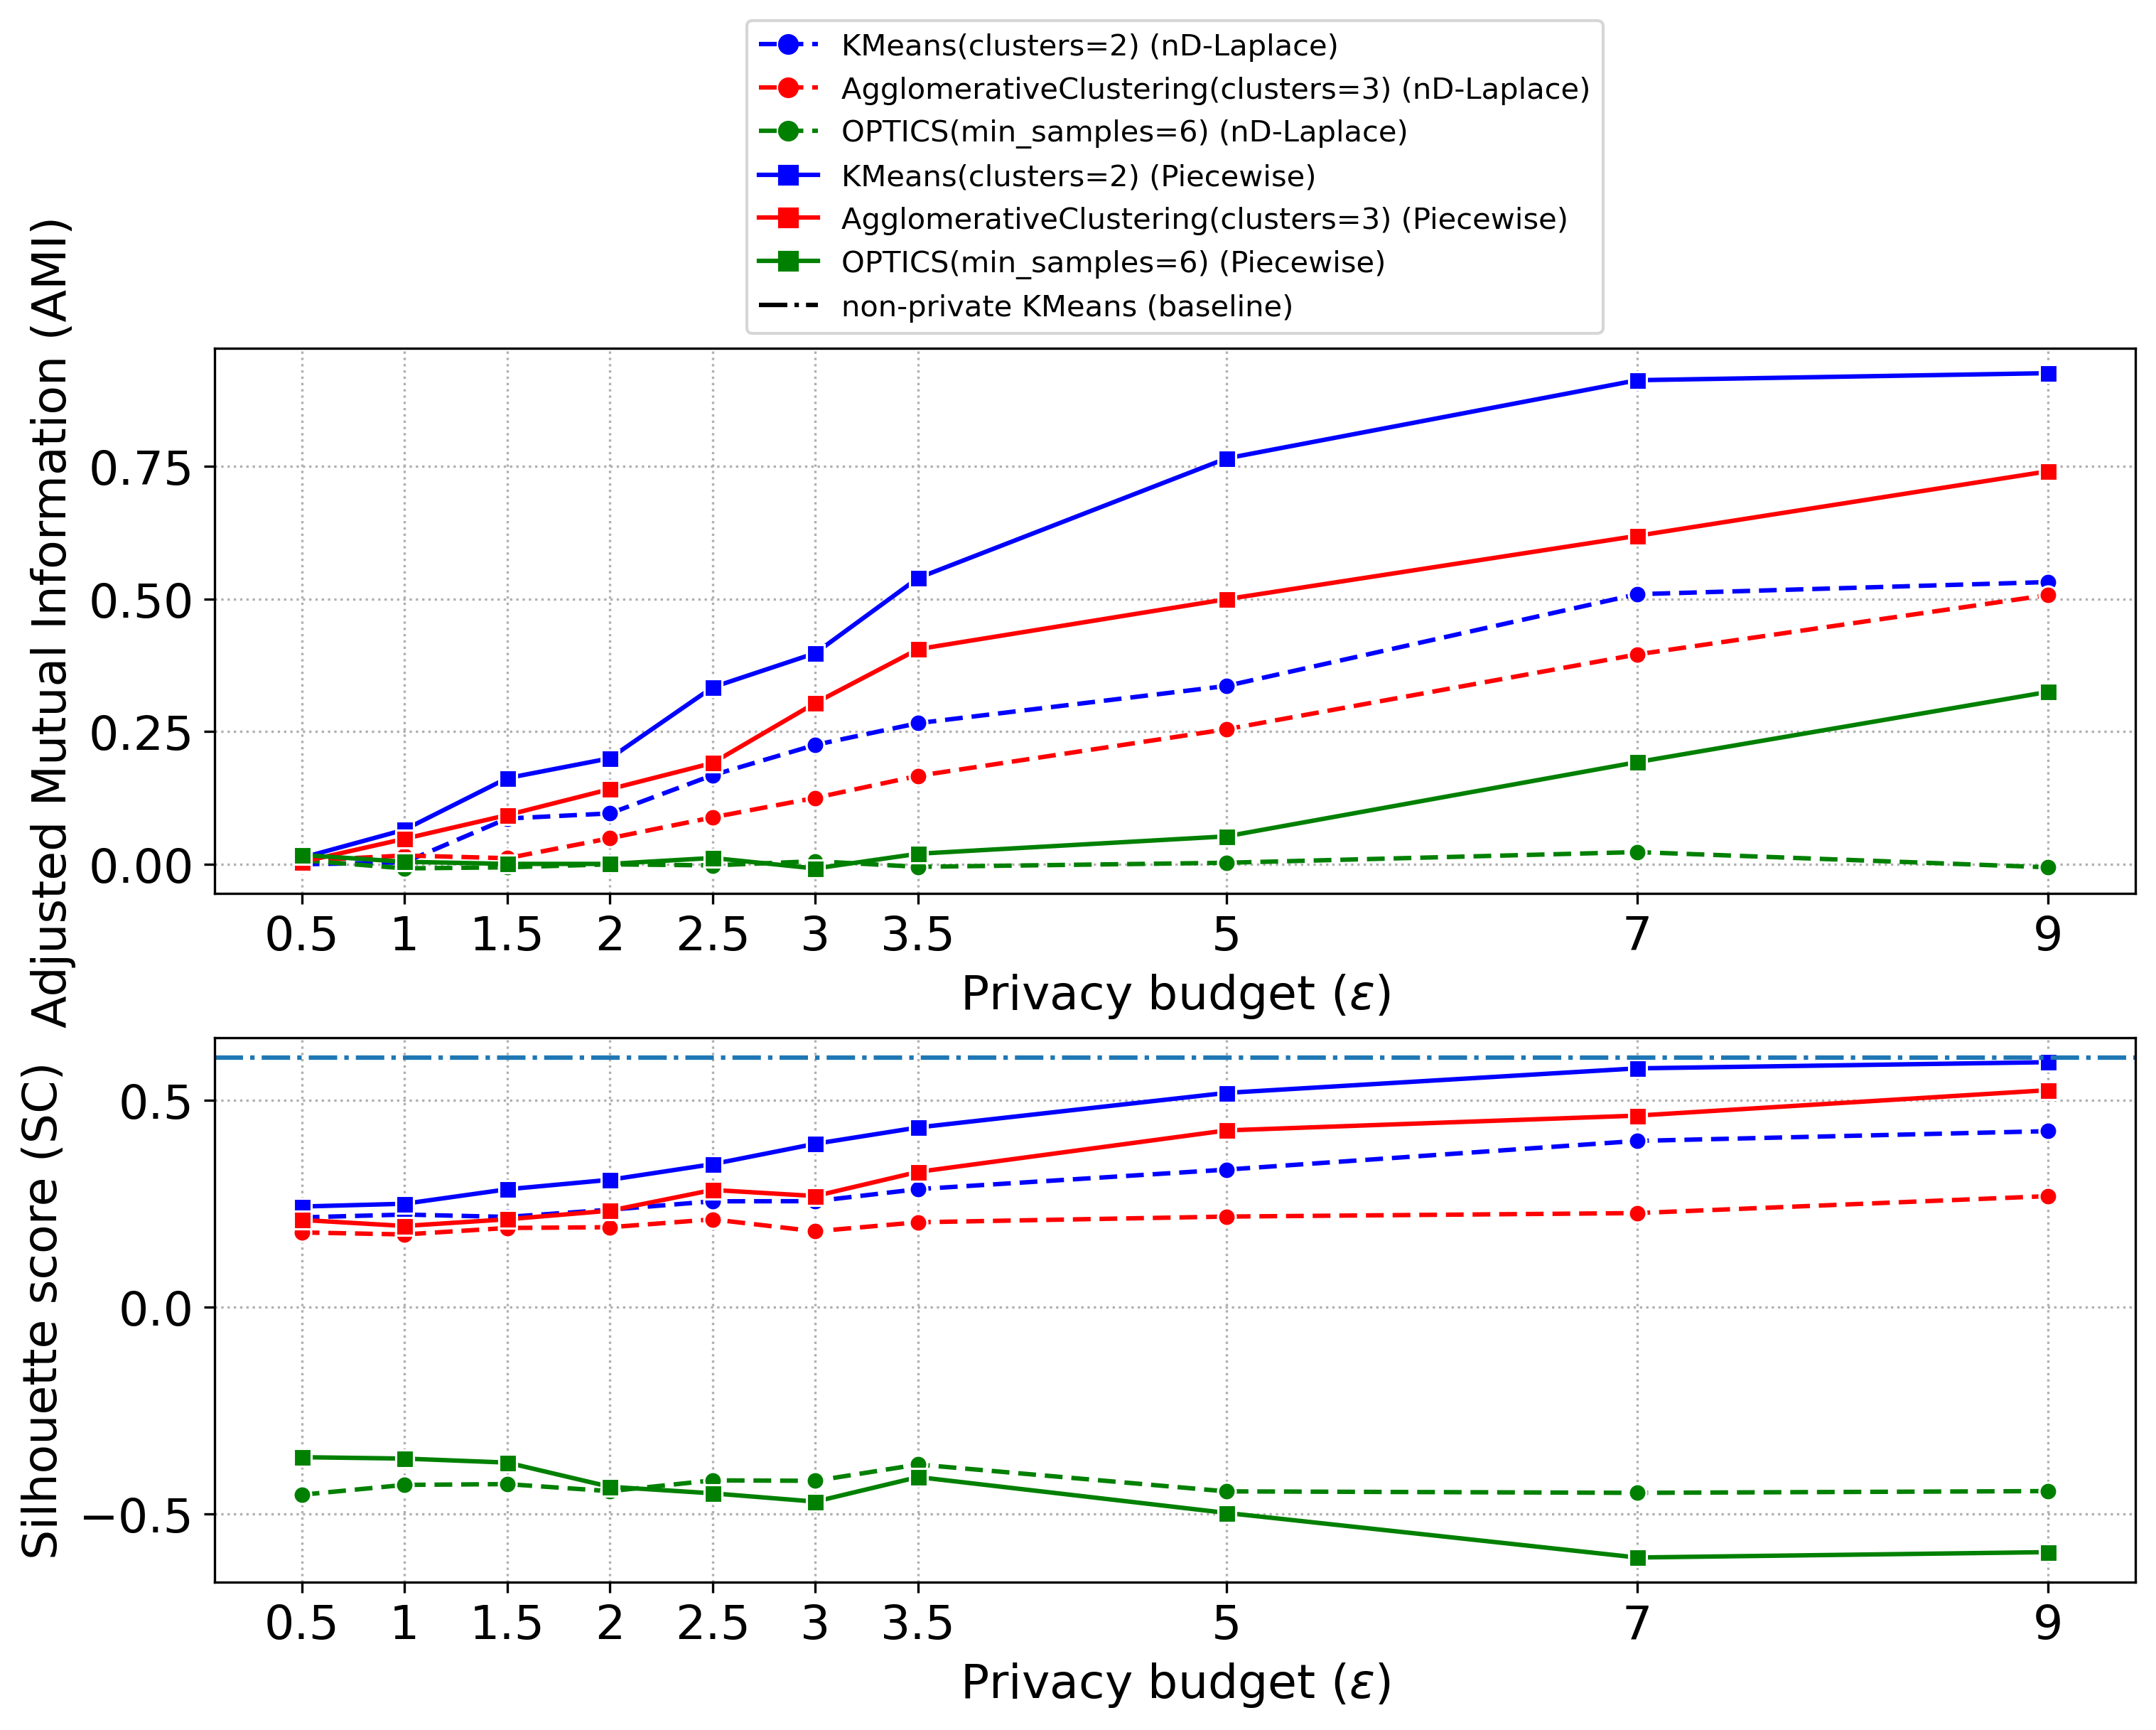
\includegraphics[width=1\textwidth]{Results/nd-laplace/nd-Laplace/line-dataset/ami-and-sc_3_dimensions.png}
  \label{fig:validation-line-dataset_comparison_3d-laplace}
\end{figure}
The scores in this plot closely resemble those from the previous one. With nD-Laplace, both K-Means and \gls{ag} lead the pack, though neither surpasses 0.6 \gls{ami}. Notably, \gls{optics} does not score at all.
The Piecewise mechanism outperforms nD-Laplace, reaching 0.86 \gls{ami} for privacy budgets at levels 7 and 9. In this scenario, \gls{ag} follows but with notably lower scores: 0.6 and 0.78 \gls{ami} for epsilon 7 and 9, respectively. While \gls{optics} remains a weaker performer across both mechanisms, it does exhibit a positive trajectory with the Piecewise mechanism.
Comparing these findings to the prior set, there are subtle variations in the \gls{sc} metric. Specifically, K-Means and \gls{ag} display a broader range of results, spanning from 0.2 to 0.6.
\newpage
\begin{figure}[H]
  \centering
  \caption{\textbf{AMI (top) and SC (bottom) for the nD-Laplace and Piecewise mechanisms for the 3-dimensional data skewed-dataset}}
  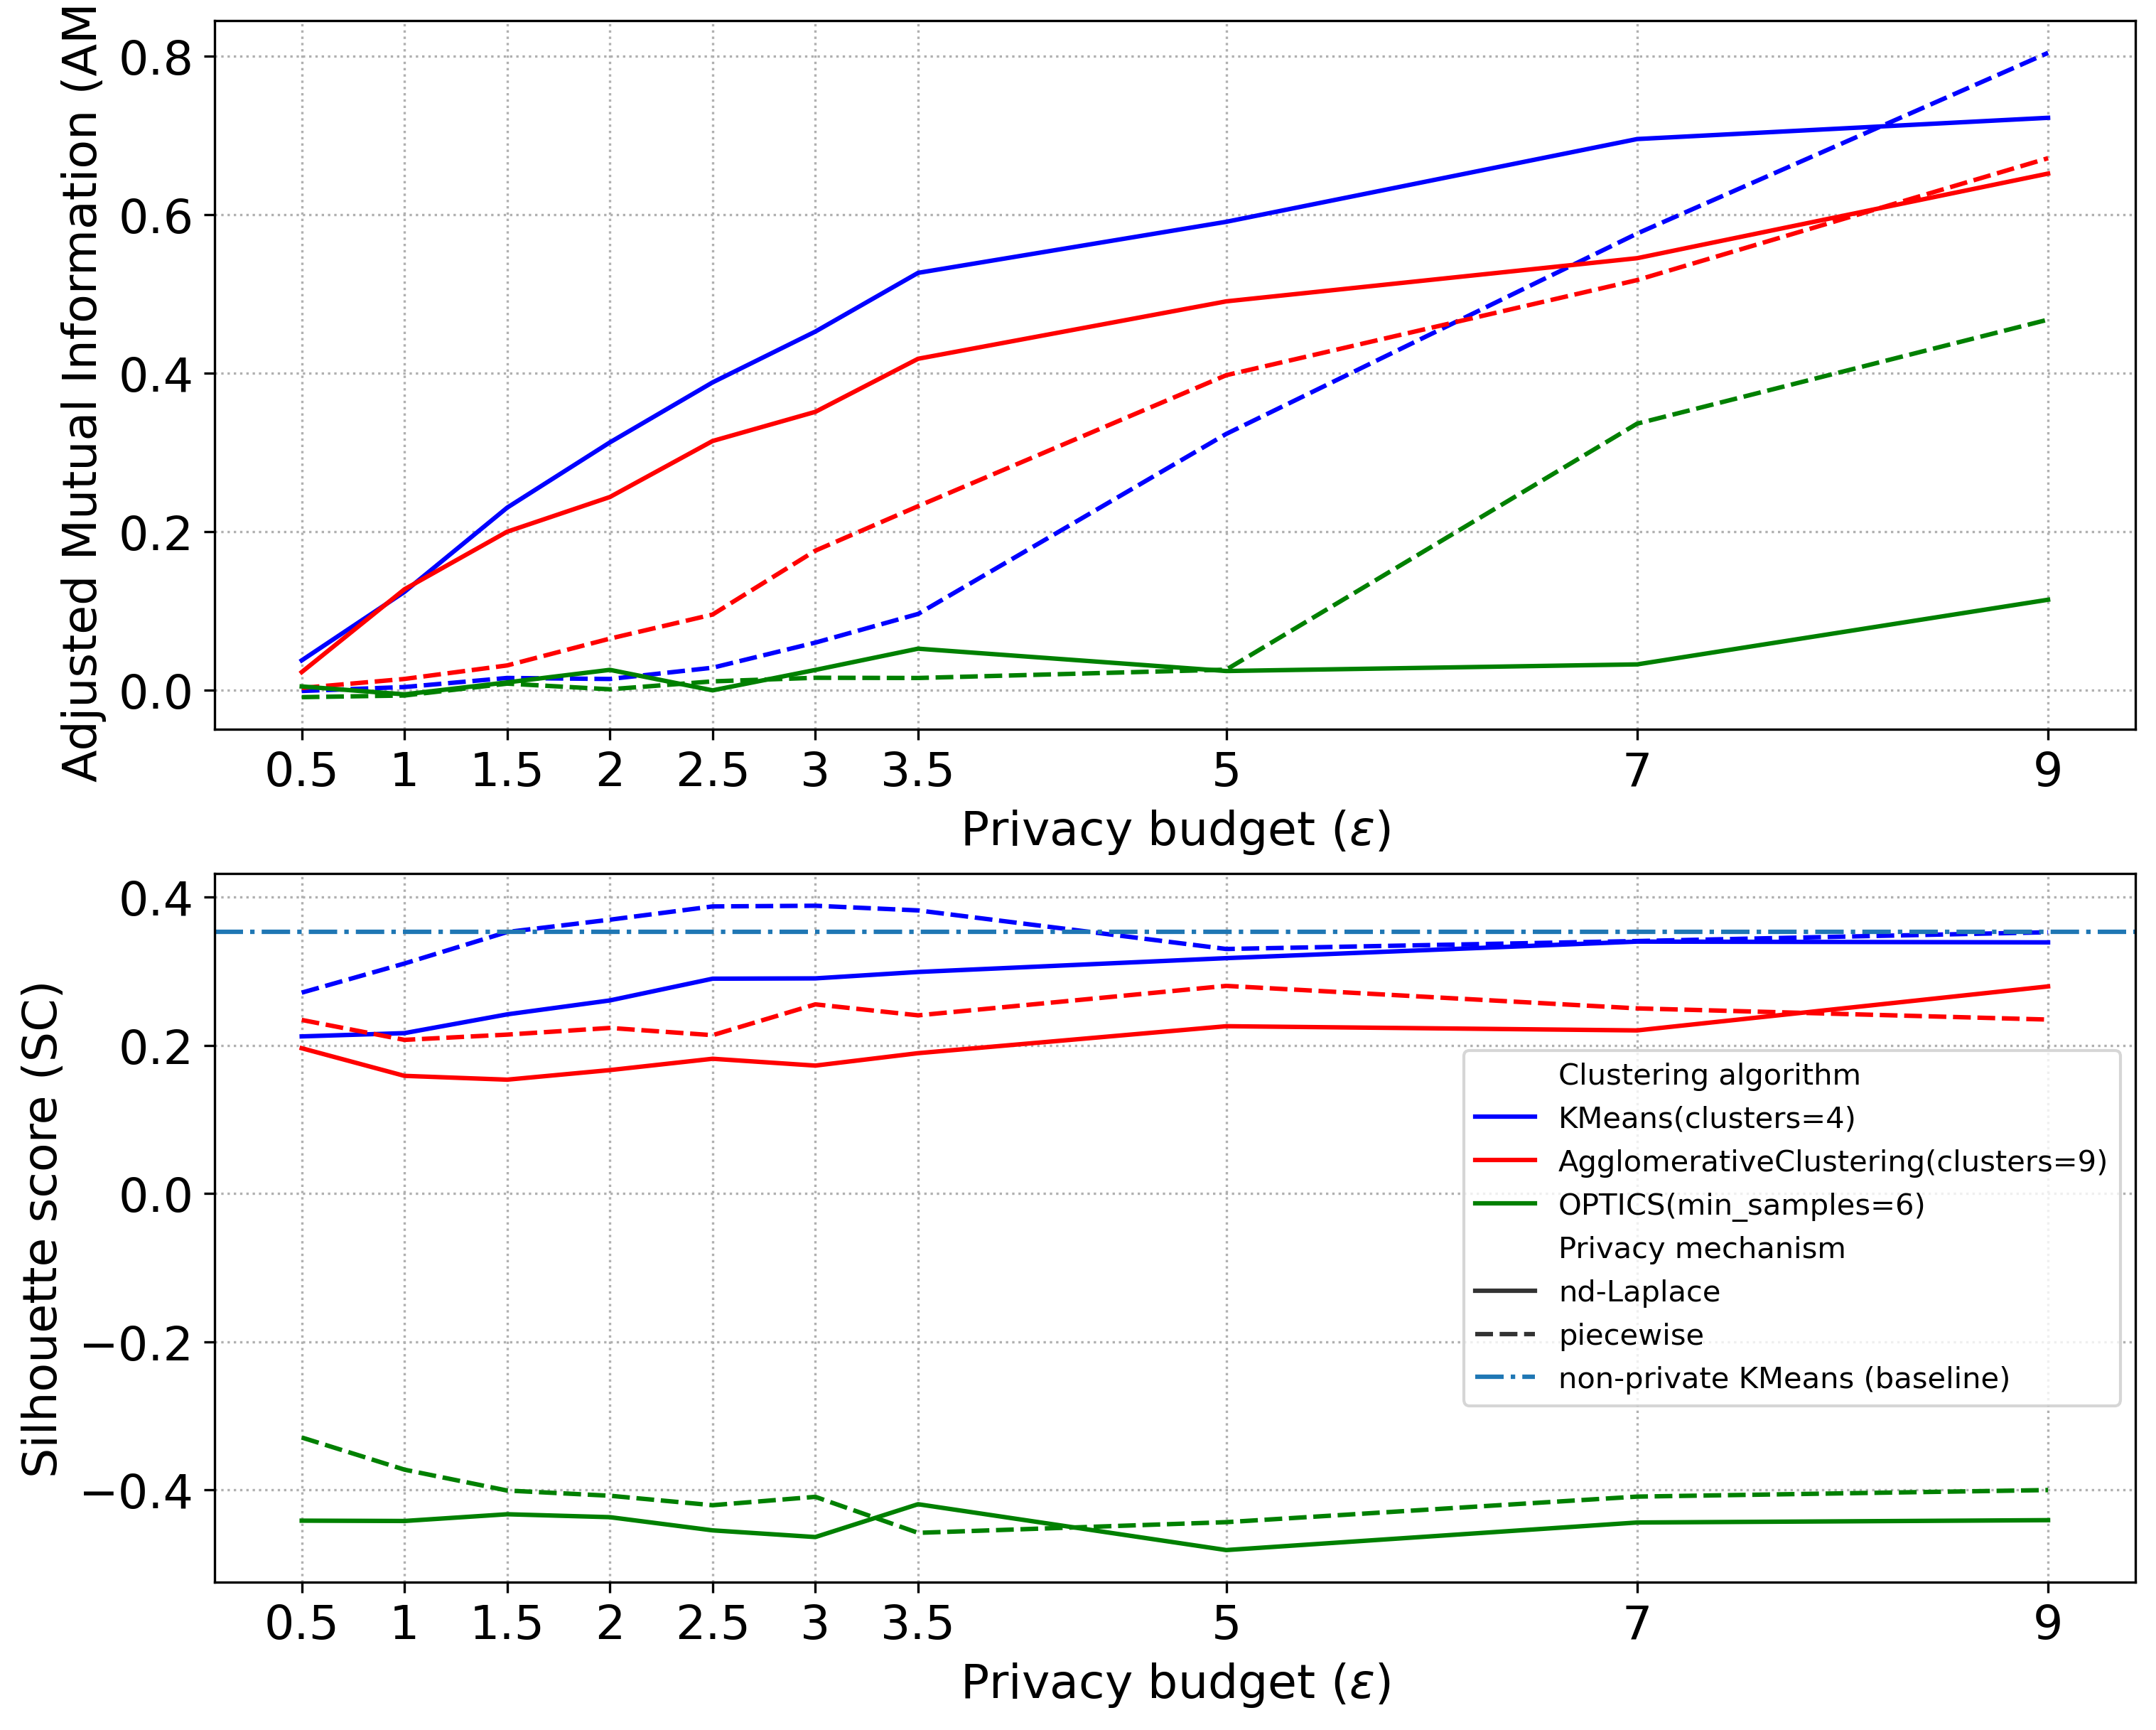
\includegraphics[width=1\textwidth]{Results/nd-laplace/nd-Laplace/skewed-dataset/ami-and-sc_3_dimensions.png}
  \label{fig:validation-skewed-dataset_comparison_3d-laplace}
\end{figure}
The nD-Laplace mechanism performs best with the K-Means algorithm, scoring approximately +/- 0.76 \gls{ami} for privacy budgets 7 and 9. \gls{ag} also scores well, reaching a maximum of 0.63 \gls{ami}. In contrast, \gls{optics} scores significantly lower.
For the Piecewise mechanism, we observe a similar pattern for K-Means and \gls{ag}. Although the progression of scores is alike, the actual scores only start to match from privacy budget 7 on wards. However, \gls{optics} scores much better from privacy budget 5.

For \gls{sc}, we see the same behavior, which we actually observe in every dataset. Both K-Means and \gls{ag} score close to the baseline value. In this case, \gls{ag} is slightly below K-Means.

From the results, it's evident that we see a similar trend in outcomes as with the heart-dataset. With nD-Laplace performing well at both lower and higher privacy budgets. When looking at the data distribution, it is spread out similarly to the heart-dataset. Whereas with the other datasets (especially circle/line), we noticed that the datasets have a strong shape.

\newpage
\subsection{n-dimensional data}
\begin{figure}[H]
  \centering

  \caption{\textbf{AMI (top) and SC (bottom) for the nD-Laplace and Piecewise mechanisms for the n-dimensional data seeds-dataset}}
  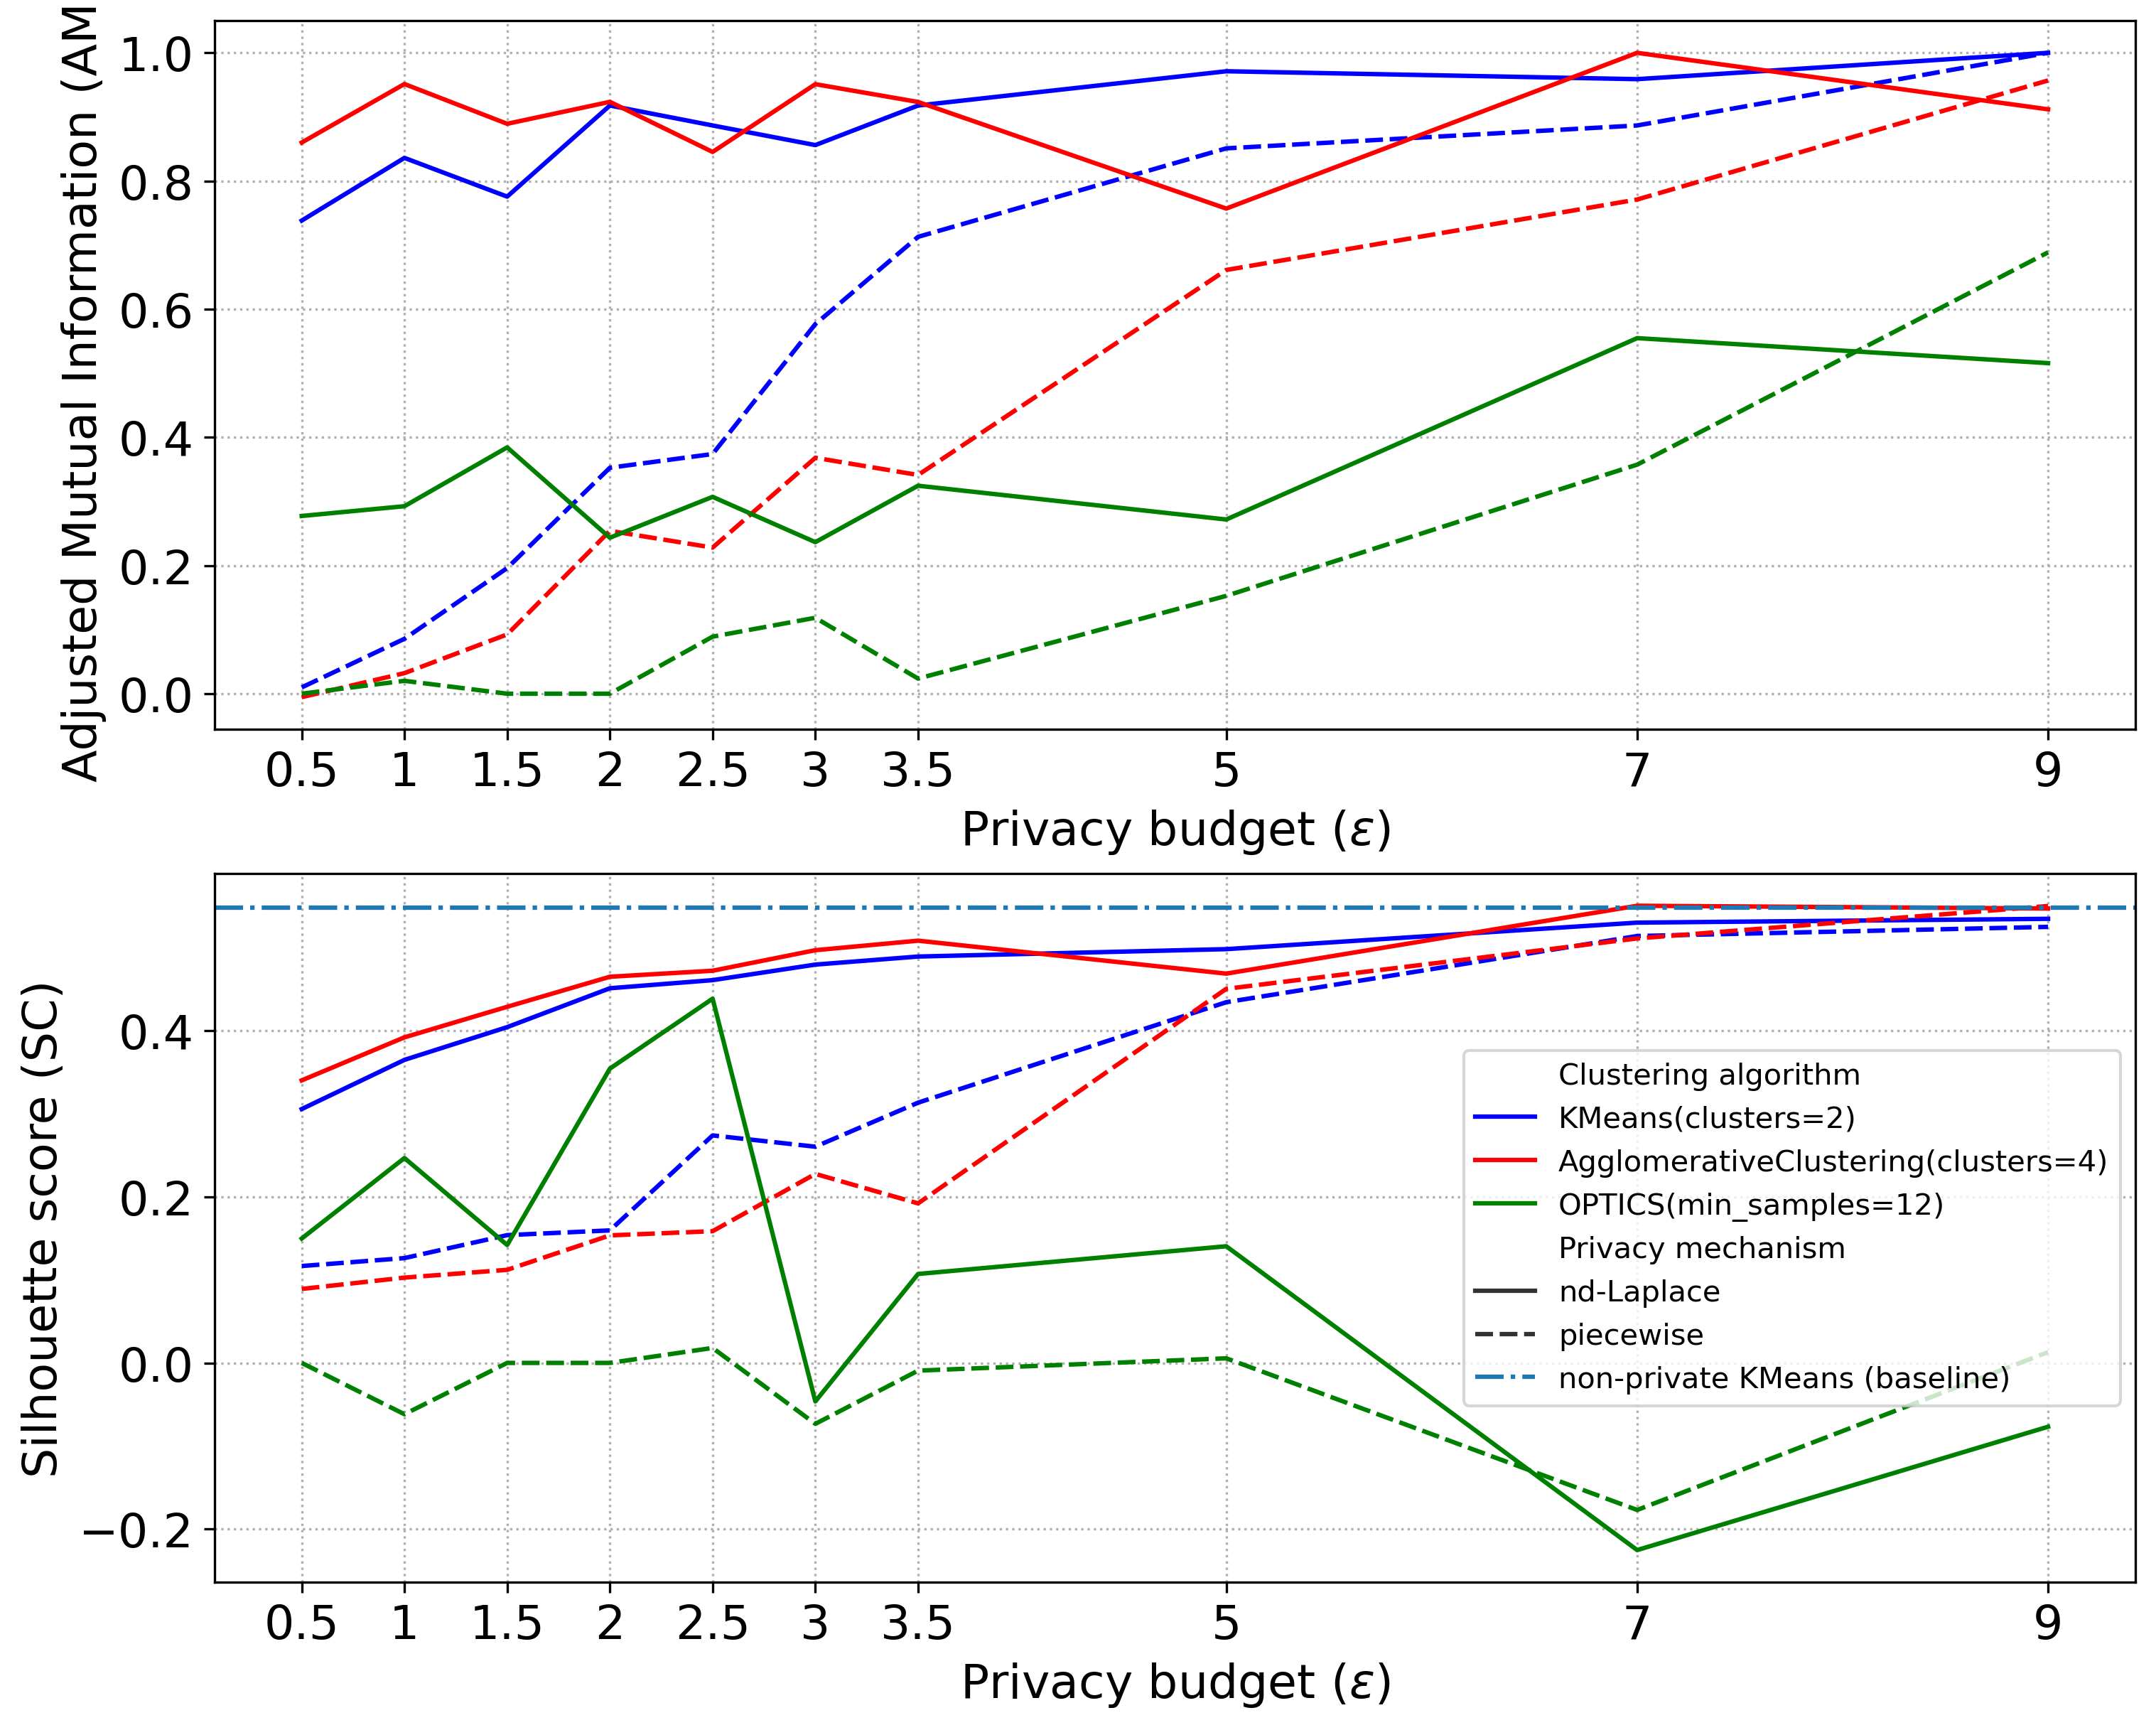
\includegraphics[width=1\textwidth]{Results/nd-laplace/nd-Laplace/seeds-dataset/ami-and-sc_7_dimensions.png}

  \label{fig:validation-seeds-dataset_comparison_nd-laplace}
\end{figure}
For n-dimensional data, we observe that nD-Laplace consistently scores high from privacy budget 0.5 up to 9. This applies to both K-Means and \gls{ag}. \gls{optics} also shows some improvements, scoring between 0.25 and 0.55 from epsilon 0.5 to 9.

The Piecewise mechanism only starts to show comparable results from a privacy budget of 5. From that point on, the results for K-Means and \gls{ag} are almost identical. For \gls{optics}, Piecewise scores slightly higher at a privacy budget of 9, but for the other privacy budgets, nD-Laplace performs better.

For \gls{sc}, we see a bit more variation between the mechanisms than with the other dimensions. Also, The trend of \gls{sc} seems more similar to that of \gls{ami} than what we've observed in other dimensions.
Looking at the scores, the nD-Laplace mechanism scores below the baseline from privacy budgets 0.5 to 7 but matches the scores for K-Means and \gls{ag} afterward. For nD-Laplace, \gls{optics} starts at 0.2 \gls{sc}, but then drops below 0. The Piecewise mechanism remains below 0 for \gls{optics} across all privacy budgets.

%Something notable occurs for the privacy budget of 2.5, as \gls{optics} peaks at 2.5. We would only expect this at a privacy budget of 9 when less noise has been added.
%\todo[inline]{We have to research this.}
% \newpage
\begin{figure}[H]
  \centering

  \caption{\textbf{AMI (top) and SC (bottom) for the nD-Laplace and Piecewise mechanisms for the n-dimensional data heart-dataset}}
  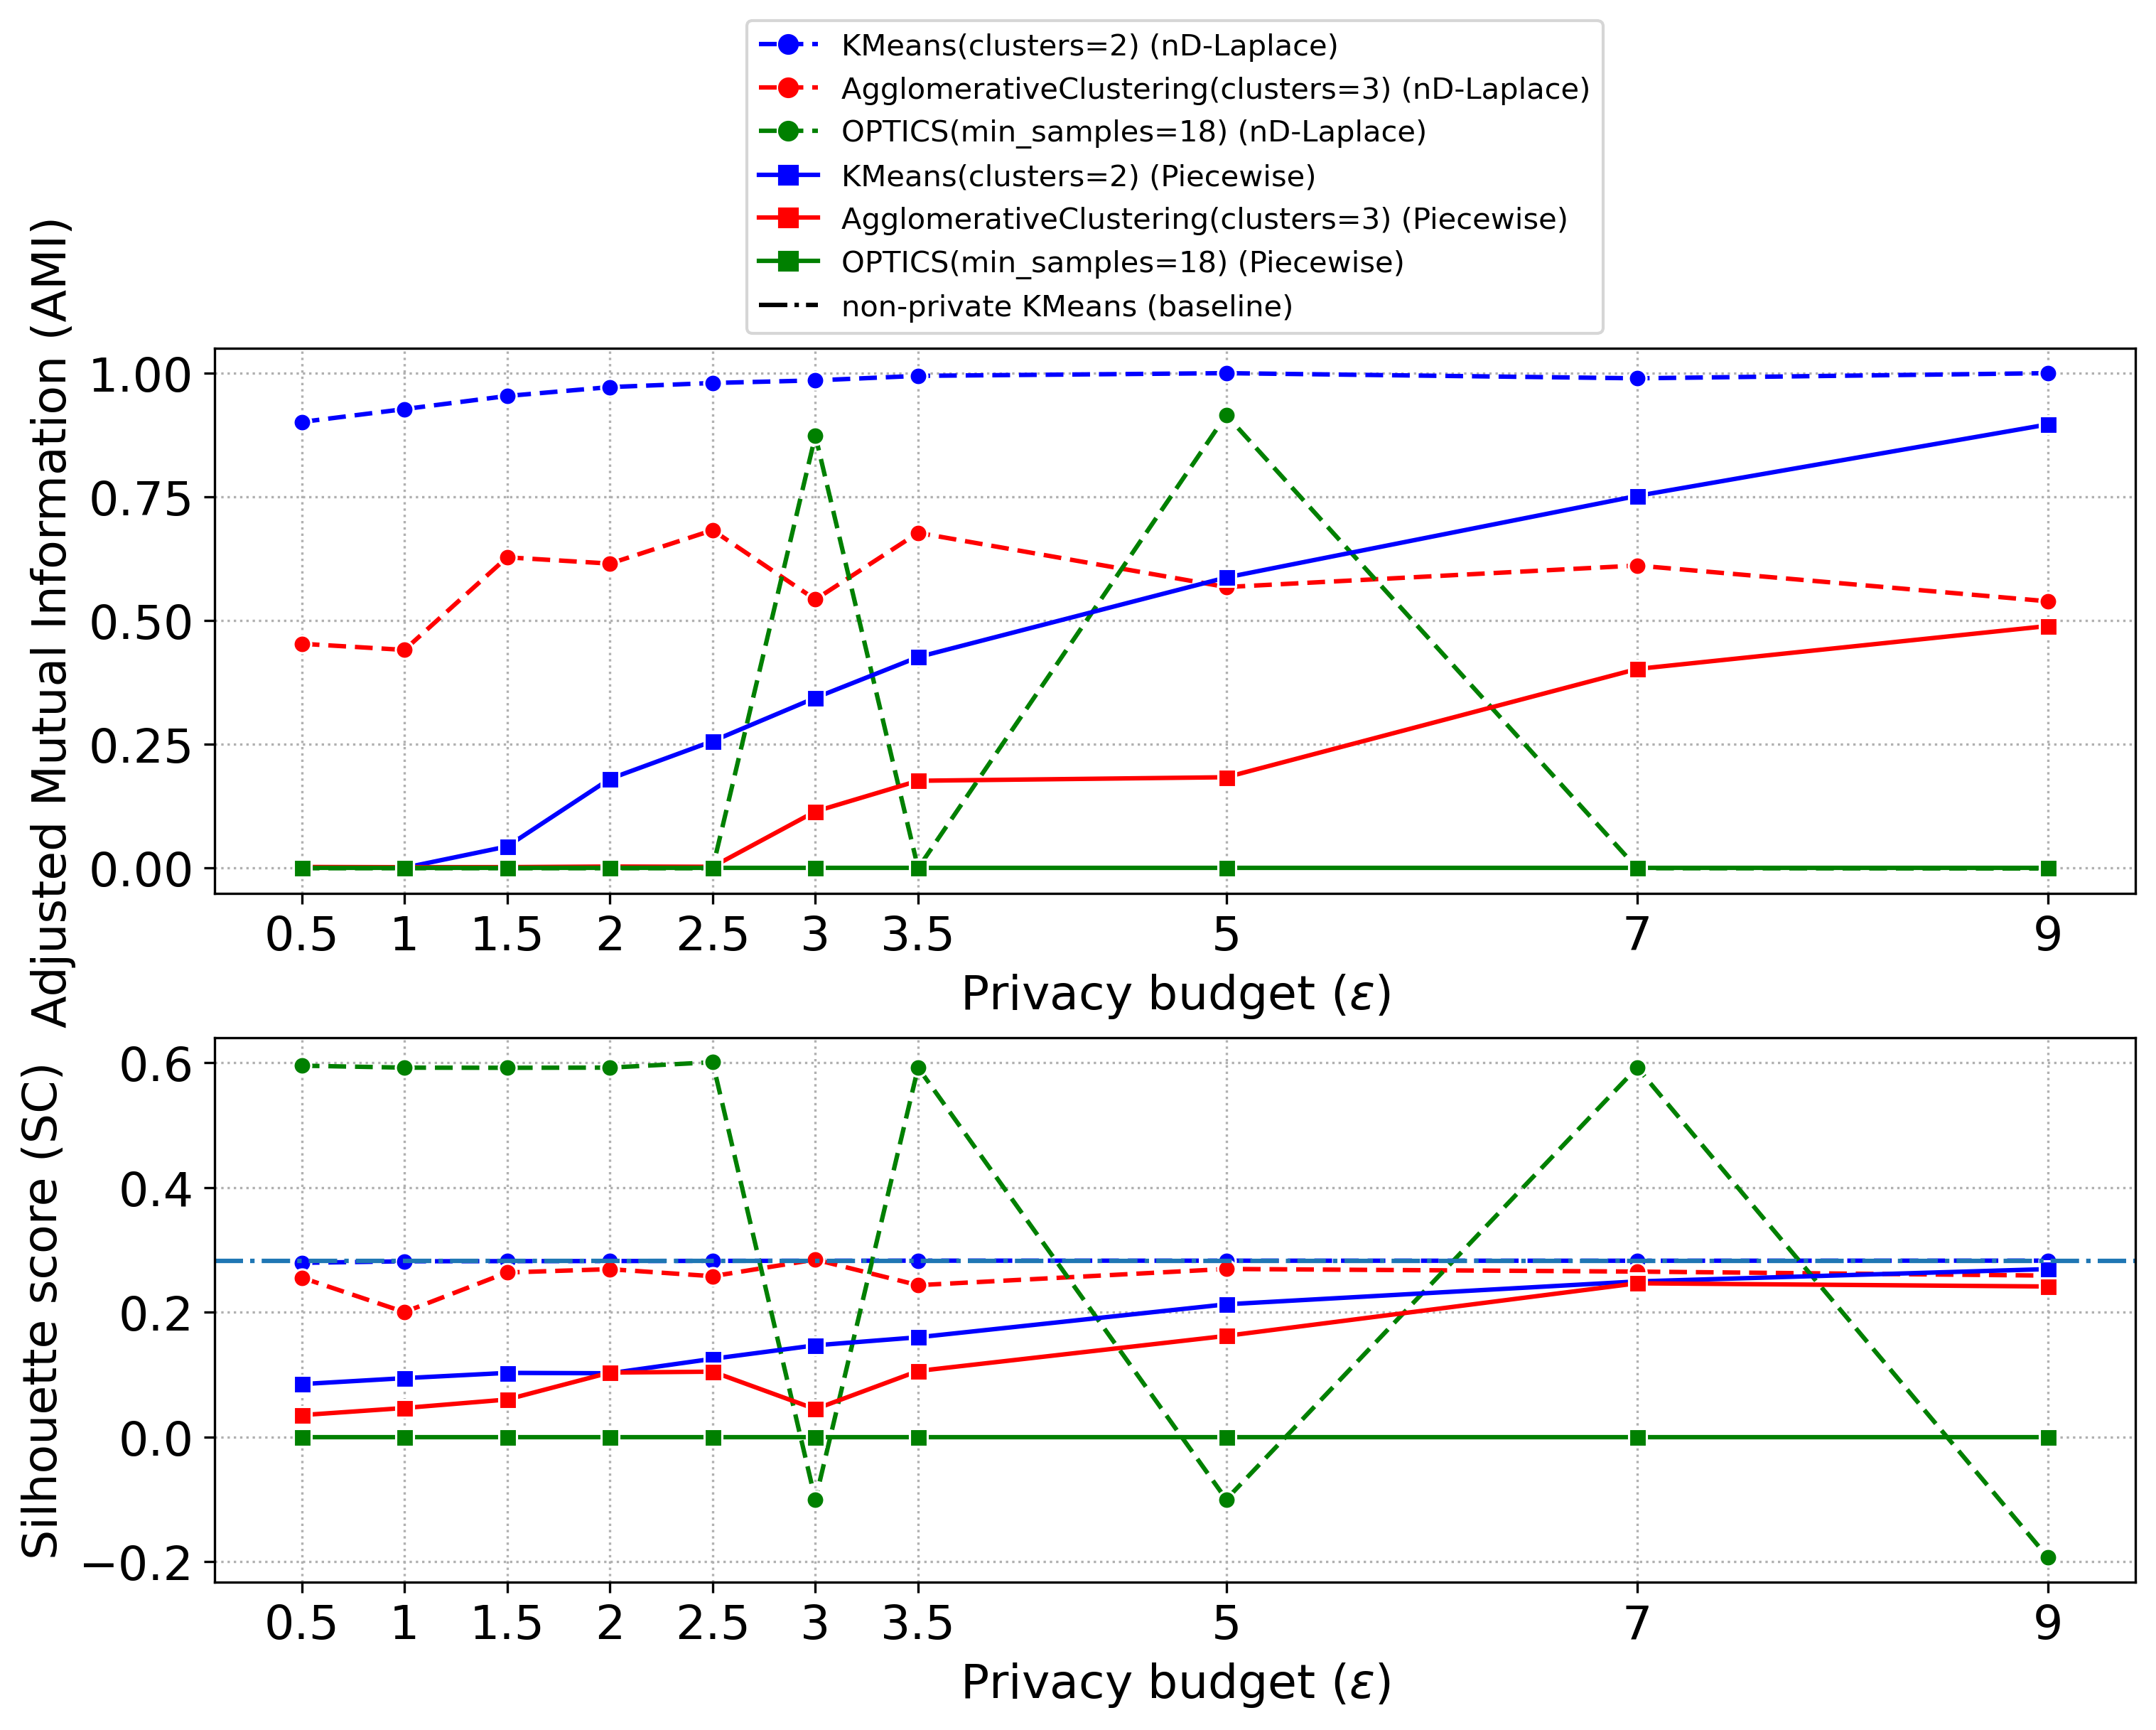
\includegraphics[width=1\textwidth]{Results/nd-laplace/nd-Laplace/heart-dataset/ami-and-sc_9_dimensions.png}

  \label{fig:validation-heart-dataset_comparison_nd-laplace}
\end{figure}
For nD-Laplace, the heart-dataset consistently scores very well for K-Means. Even for n-dimensional data, the result consistently remains above 0.95 \gls{ami} for all privacy budgets.
For \gls{ag}, a good score is achieved, but it plateaus around 0.6 \gls{ami}.
With \gls{optics}, the data is quite inconsistent, ranging from 0 to 0.90 \gls{ami}.
The Piecewise mechanism shows a similar trend for both K-Means and \gls{ag}, with K-Means performing the best. Both score below nD-Laplace across all privacy budgets.
For \gls{optics}, the score remains at 0 for the Piecewise mechanism.
With the \gls{sc} metric, the same pattern is evident, but the \gls{sc} is relatively low when considering the high \gls{ami} achieved. For \gls{optics}, an odd result is observed, as it scores 0.6 \gls{ami} (0.25 above the baseline) from 0.5 to 3. However, for privacy budgets of 3, 5, and 9, the score drops back to 0 \gls{sc}.

\newpage
\section{Mechanism utility}
The sections below present a heatmap comparison of the nd-Laplace and Piecewise mechanisms.
We employed a heatmap to simultaneously depict the privacy budget (epsilon), the number of dimensions, and a specific metric. The metric in focus is the \gls{ami}, which is determined using the K-Means algorithm.
We opted for K-Means as it consistently delivered reliable results across all our experiments, making it an ideal baseline for gauging the \gls{ami}.

On the heatmap, the x-axis represents the privacy budget, while the y-axis illustrates the number of dimensions. Each cell of the heatmap conveys the \gls{ami} value. The intensity of the cell's color corresponds to the \gls{ami} score: a darker shade signifies a higher score. Consequently, the darker (or higher) the score, the more favorable the outcome. \newline

The results for the shape datasets (Circle, Line and Skewed) were omitted, because we do not have more then 3 dimensions. Therefore, the heat maps do not yield a lot of information in addition to the cluster utility plots.

Please refer to the plots in the appendix for:
\begin{enumerate}
  \item Privacy distance: Appendix:\ref{appendix:results-privacy}.
  \item True Positive Rate: Appendix: \ref{appendix:results-privacy}.
\end{enumerate}
\newpage
\subsection{Seeds-dataset}
\begin{figure}[H]
  \centering
  \begin{subfigure}[b]{0.8\textwidth}
    \begin{subfigure}[c]{1\textwidth}
      \caption{\textbf{Adjusted Mutual Information comparison for the nD-Laplace mechanism}}
      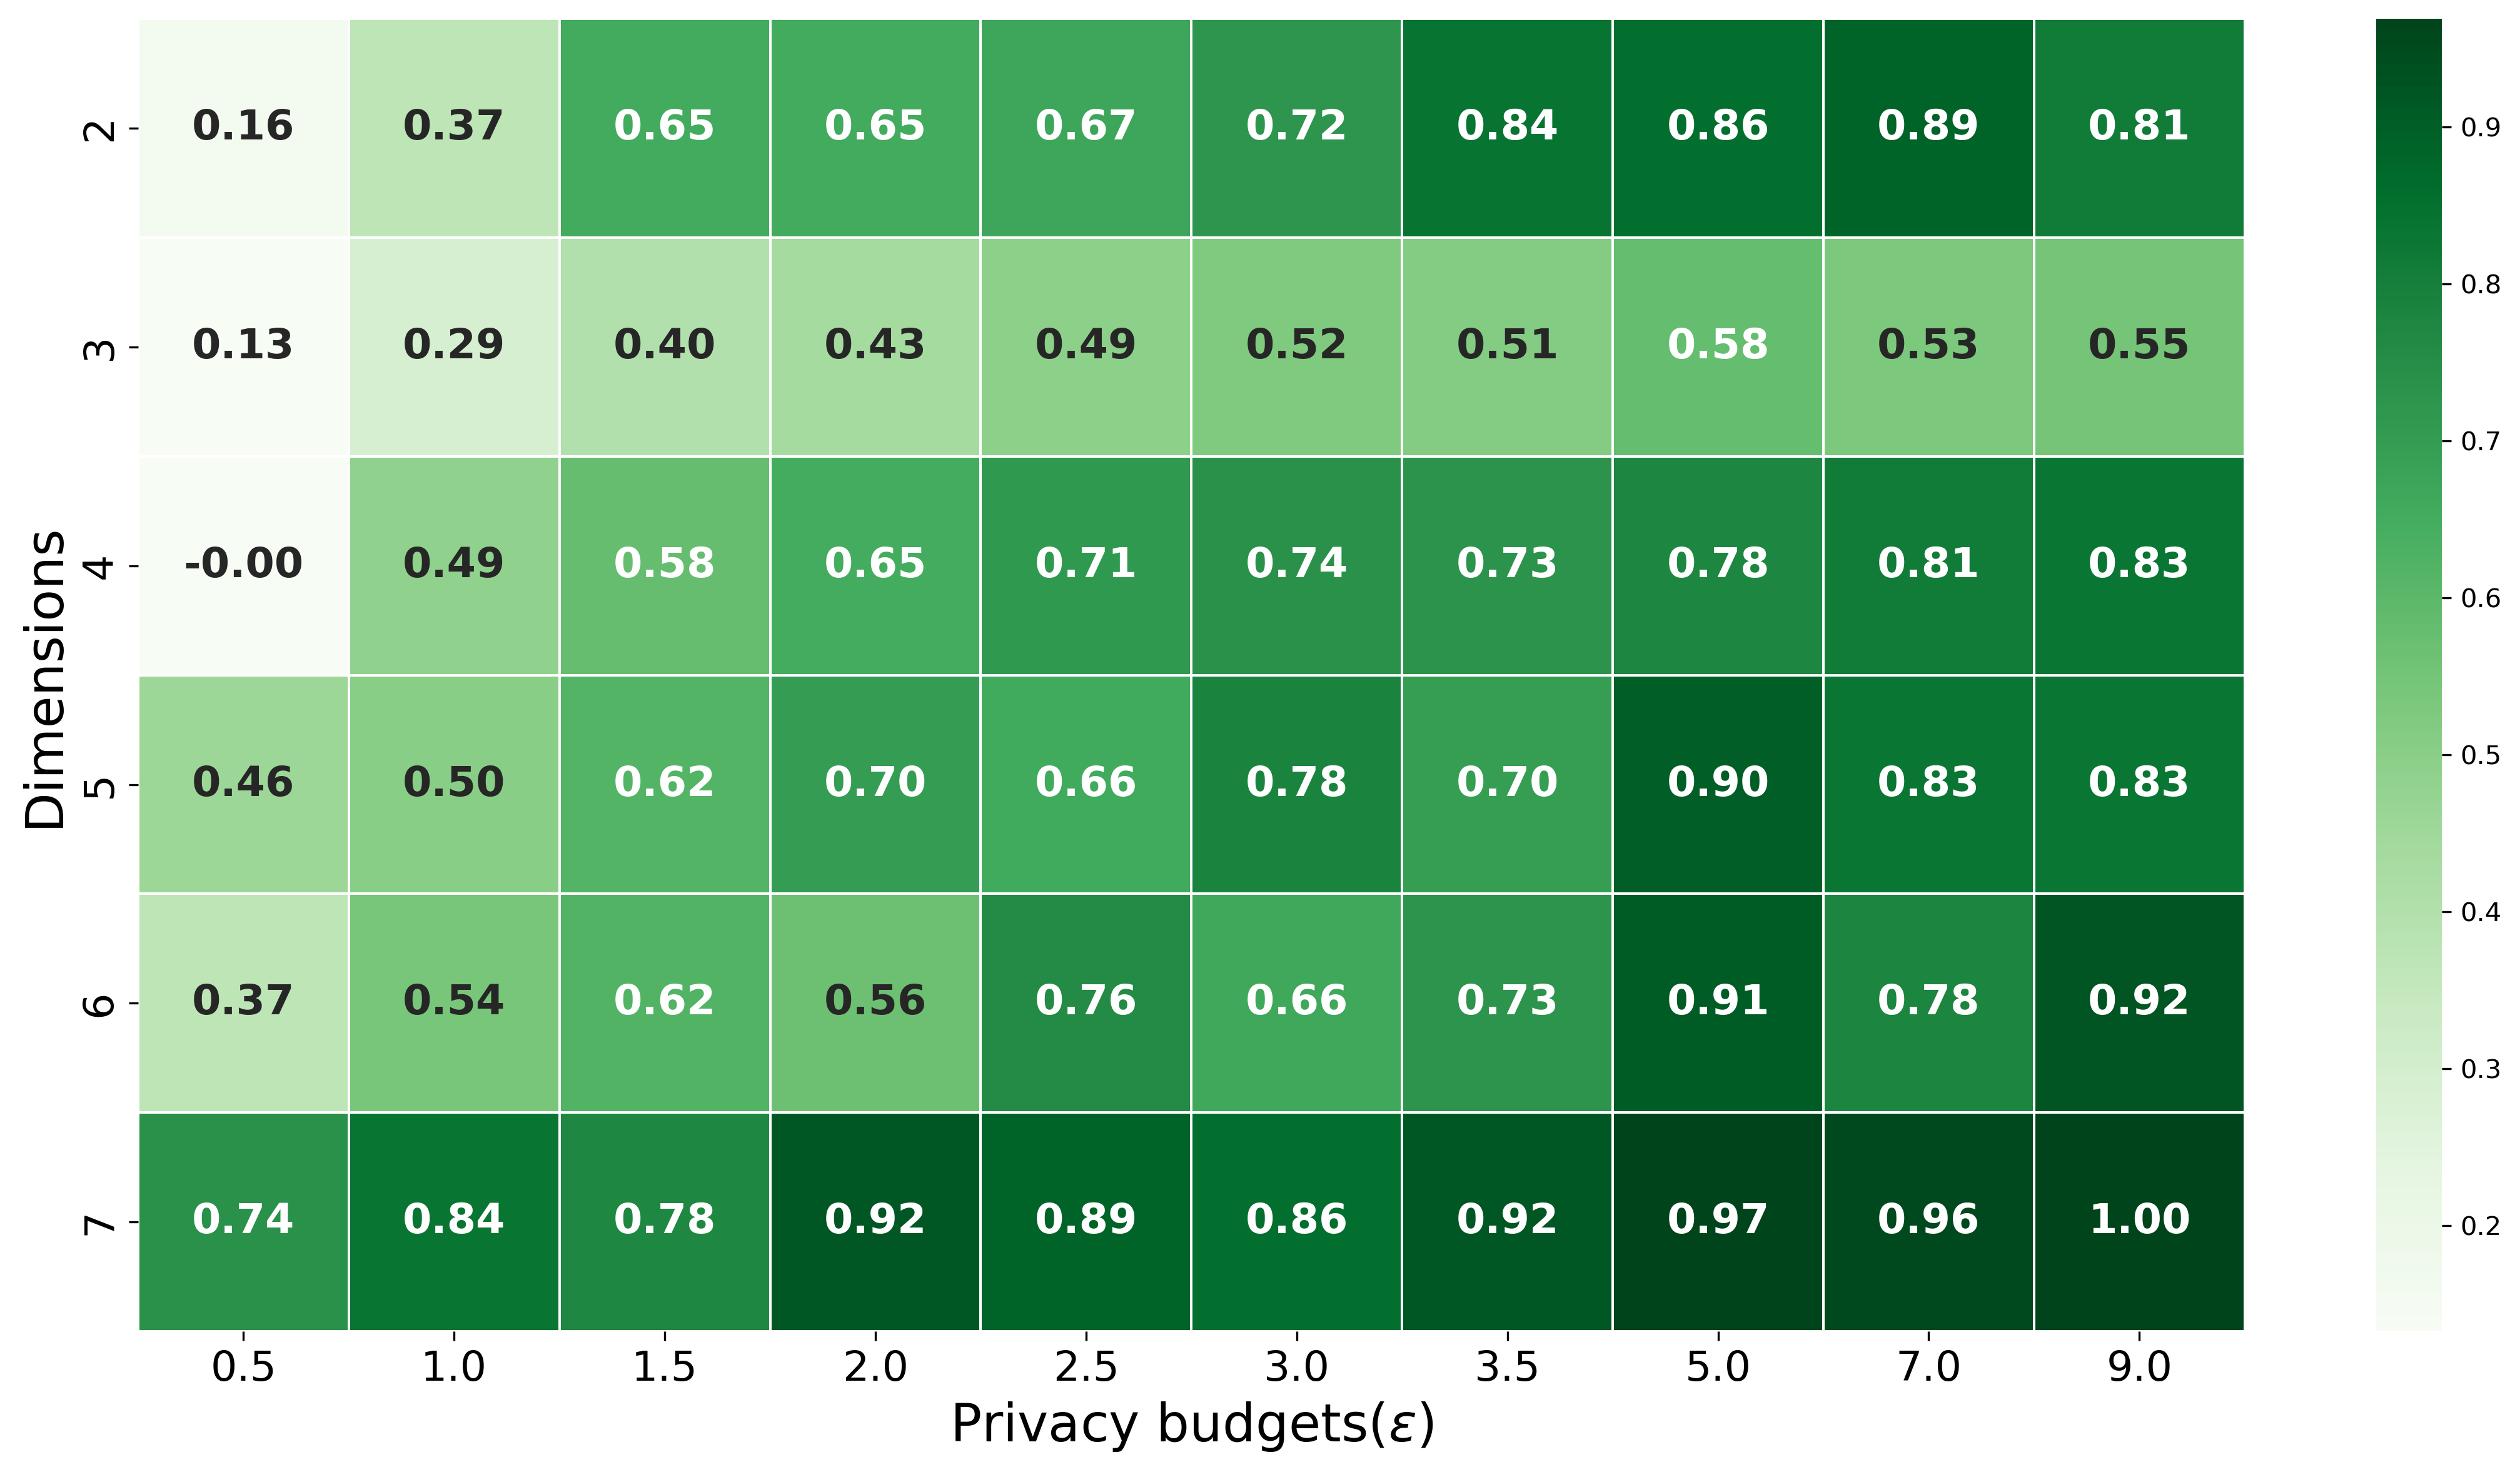
\includegraphics[width=1\textwidth]{Results/nd-laplace/nd-Laplace/seeds-dataset/ami.png}
      \label{fig:ami_seeds-dataset_comparison_kdlaplace_2d}
    \end{subfigure}
    \vfill % vertical space
    \begin{subfigure}[c]{1\textwidth}
      \caption{\textbf{Adjusted Mutual Information comparison for the Piecewise mechanism}}
      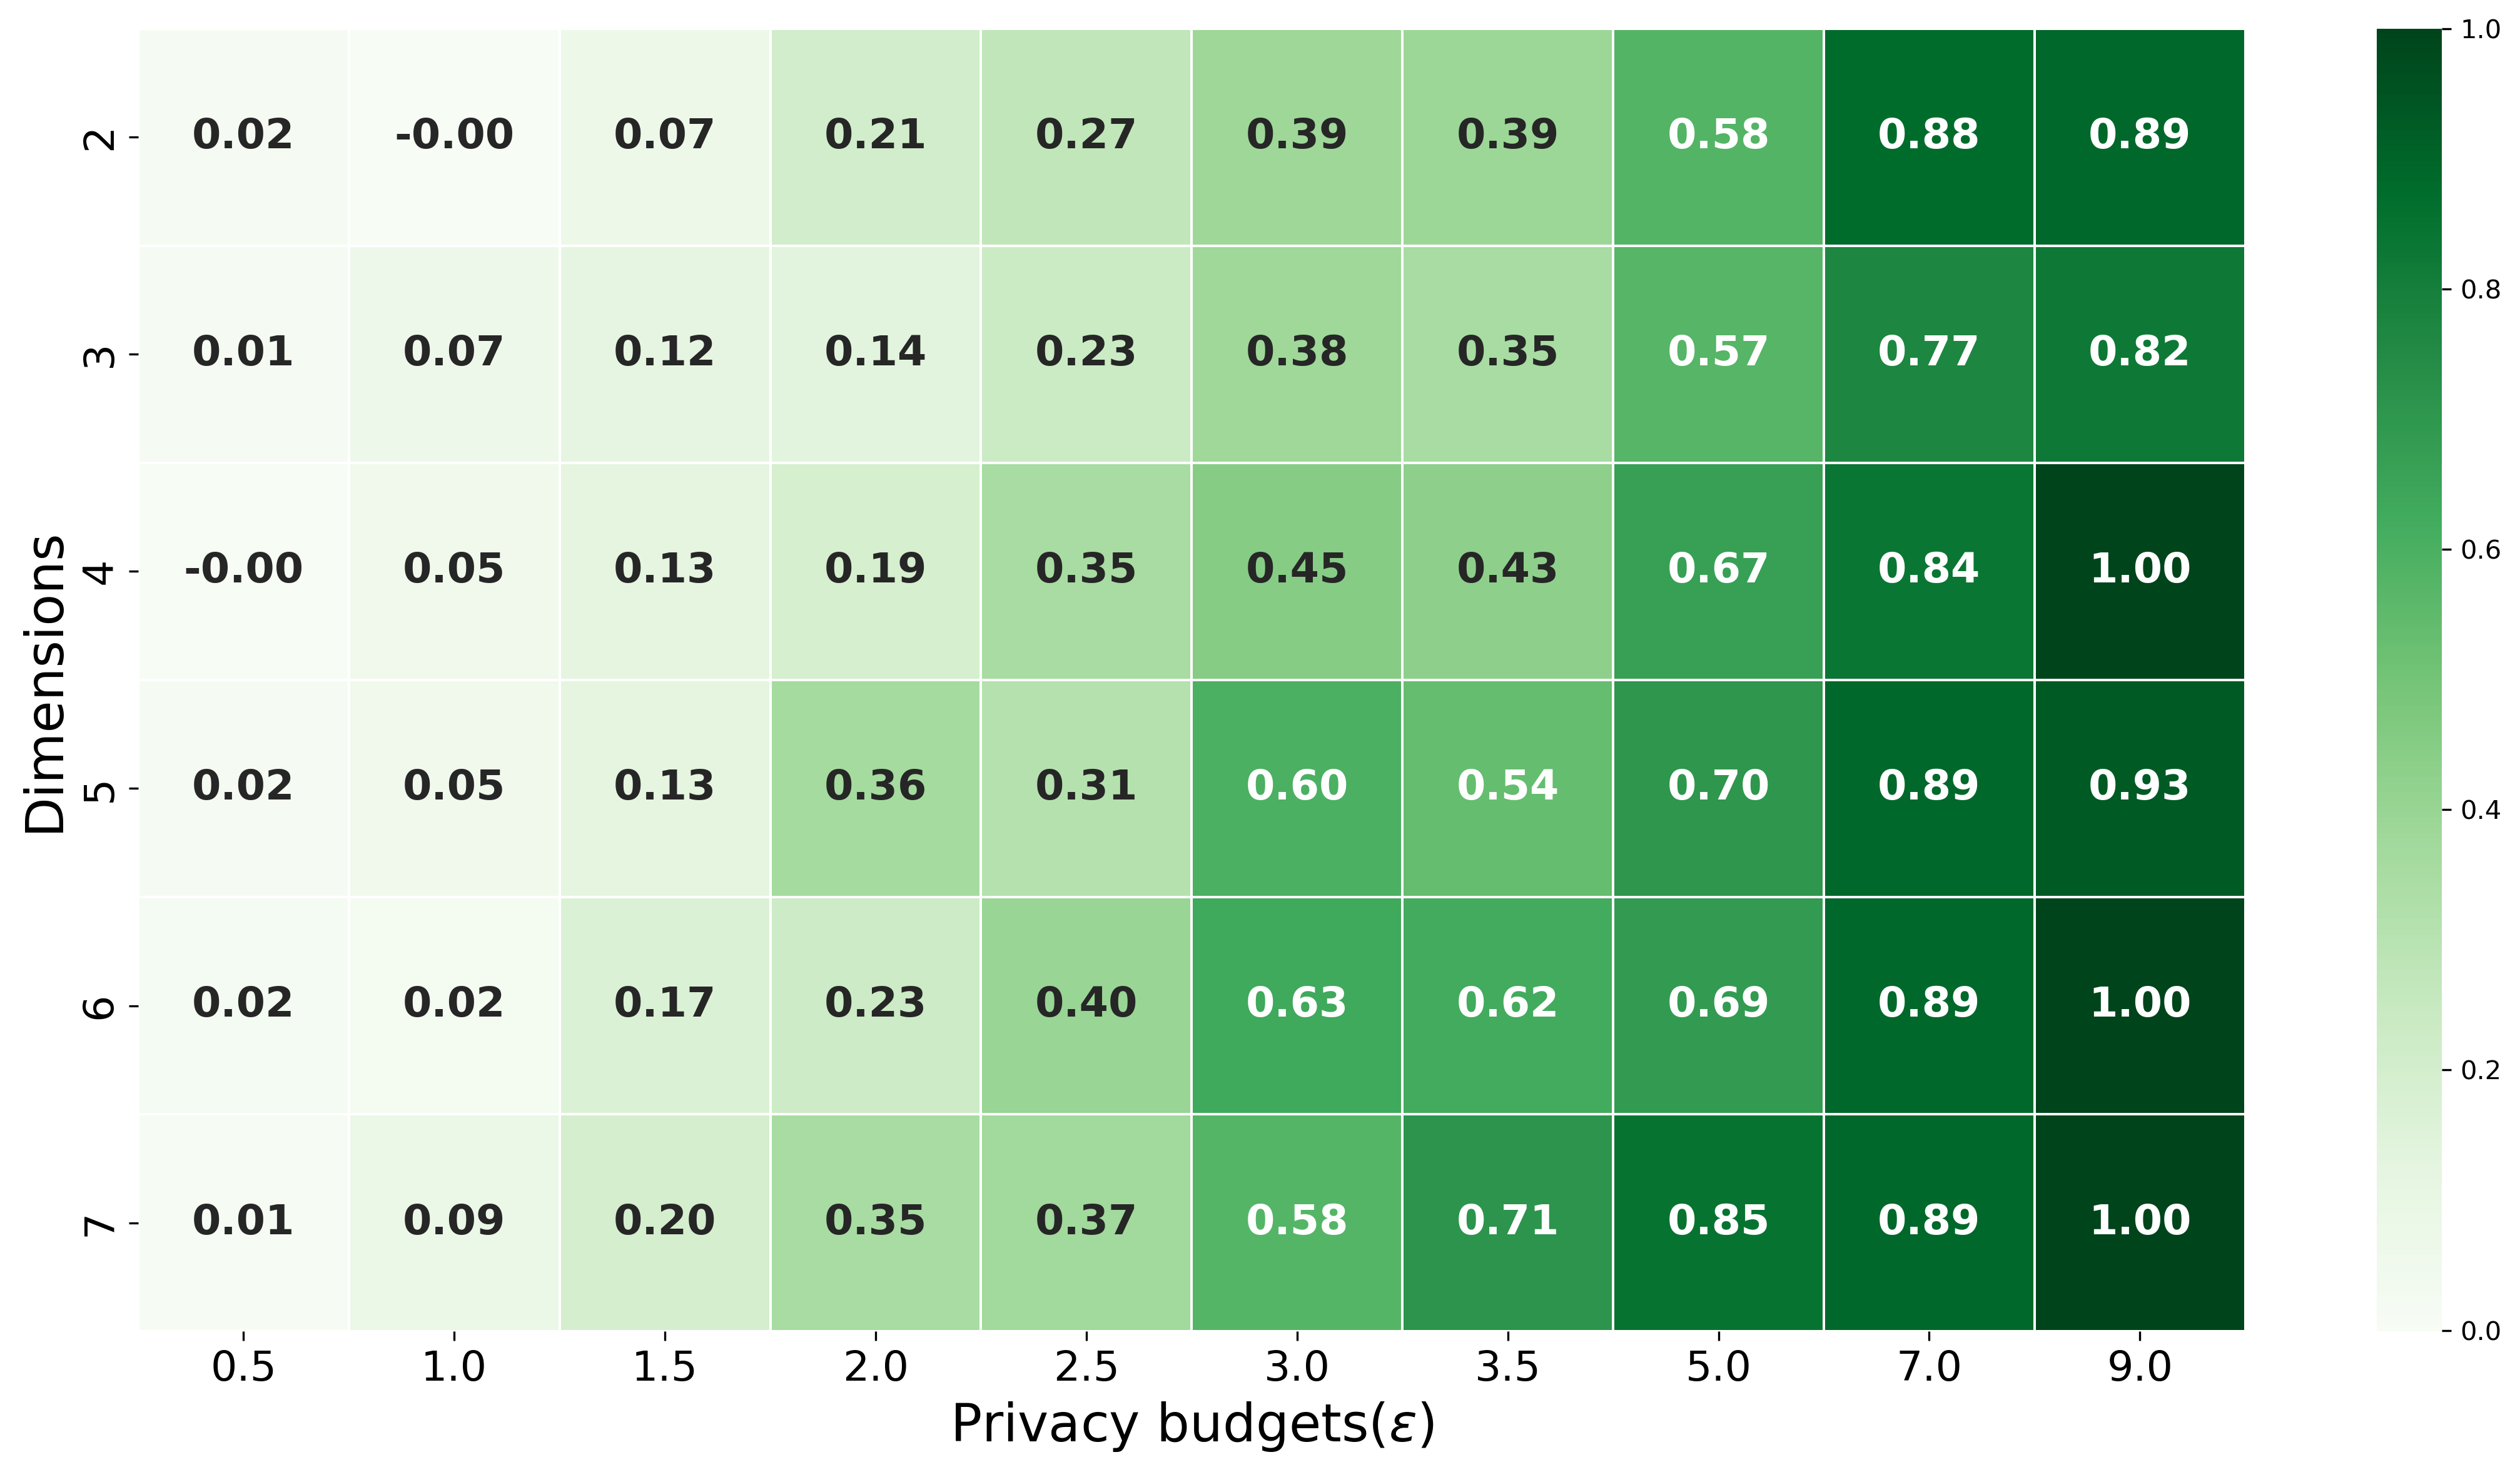
\includegraphics[width=1\textwidth]{Results/nd-laplace/piecewise/seeds-dataset/ami.png}
      \label{fig:ami_seeds-dataset_comparison_piecewise_2d}
    \end{subfigure}
  \end{subfigure}

\end{figure}
For the heatmaps, we observe a similar pattern, which was also evident in the cluster analysis. Specifically, nD-Laplace consistently scores well from lower epsilons, while Piecewise only starts to perform well from a privacy budget of 3.
For nD-Laplace, the number of dimensions influences the score. The implementation of 3D-Laplace, in particular, scores relatively low. From 4 dimensions onward, we notice an increase in the \gls{ami}, especially in combination with an increasing privacy budget.
For Piecewise, it's notable that the number of dimensions has minimal impact on the outcome, with the privacy budget being the primary influencing factor. However, dimension does play a role for privacy budgets between 3 and 5, as scores are higher from 5 dimensions compared to lower dimensions.

For nD-Laplace, the dimensions can significantly influence the improved result because as the number of dimensions increases, the noise decreases. We've elaborated on this phenomenon in Section \ref{fig:curse-of-dimensionality}. As a result, more information is retained, leading to an increase in score with the number of dimensions. The Piecewise mechanism might also be affected by this, but to a lesser extent.
% \todo[inline]{Further research needed}

\newpage
\subsection{Heart-dataset}
\begin{figure}[H]
  \centering
  \begin{subfigure}[b]{0.80\textwidth}
    \begin{subfigure}[c]{1\textwidth}
      \caption{\textbf{Adjusted Mutual Information comparison for the nD-Laplace mechanism}}
      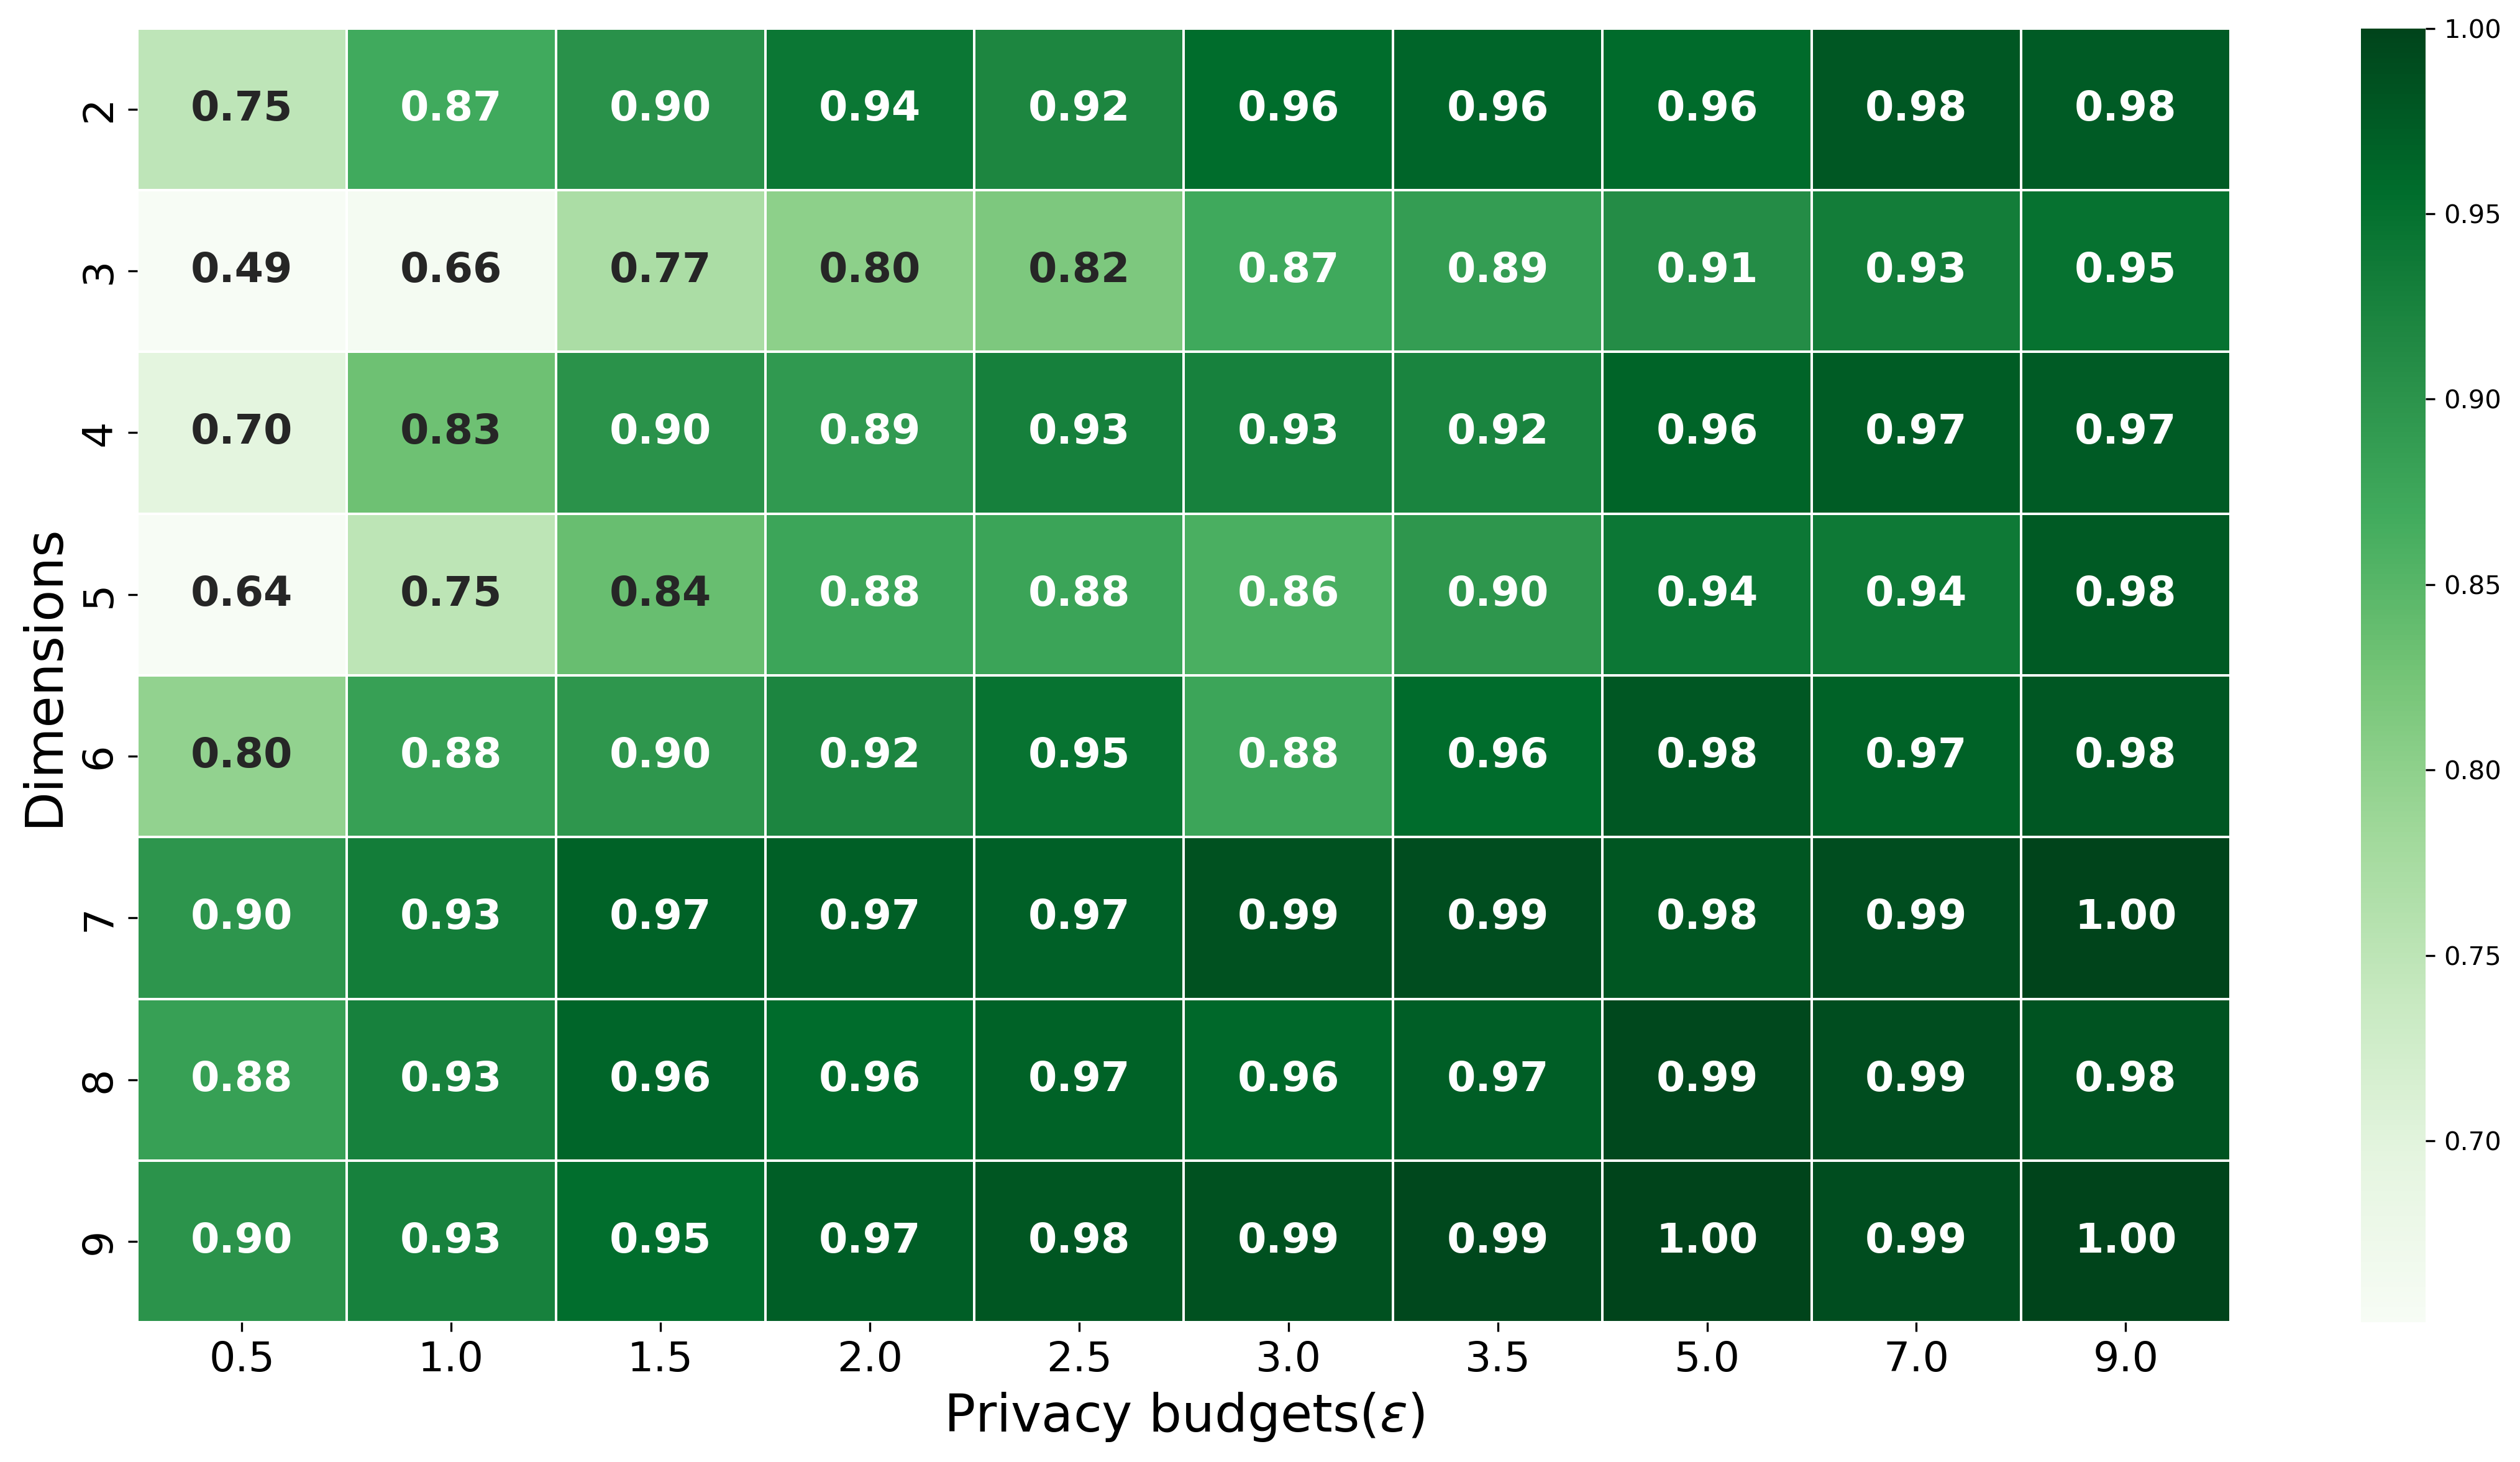
\includegraphics[width=1\textwidth]{Results/nd-laplace/nd-Laplace/heart-dataset/ami.png}
      \label{fig:ami_heart-dataset_comparison_kdlaplace_2d}
    \end{subfigure}
    \vfill % vertical space
    \begin{subfigure}[c]{1\textwidth}
      \caption{\textbf{Adjusted Mutual Information comparison for the Piecewise mechanism}}
      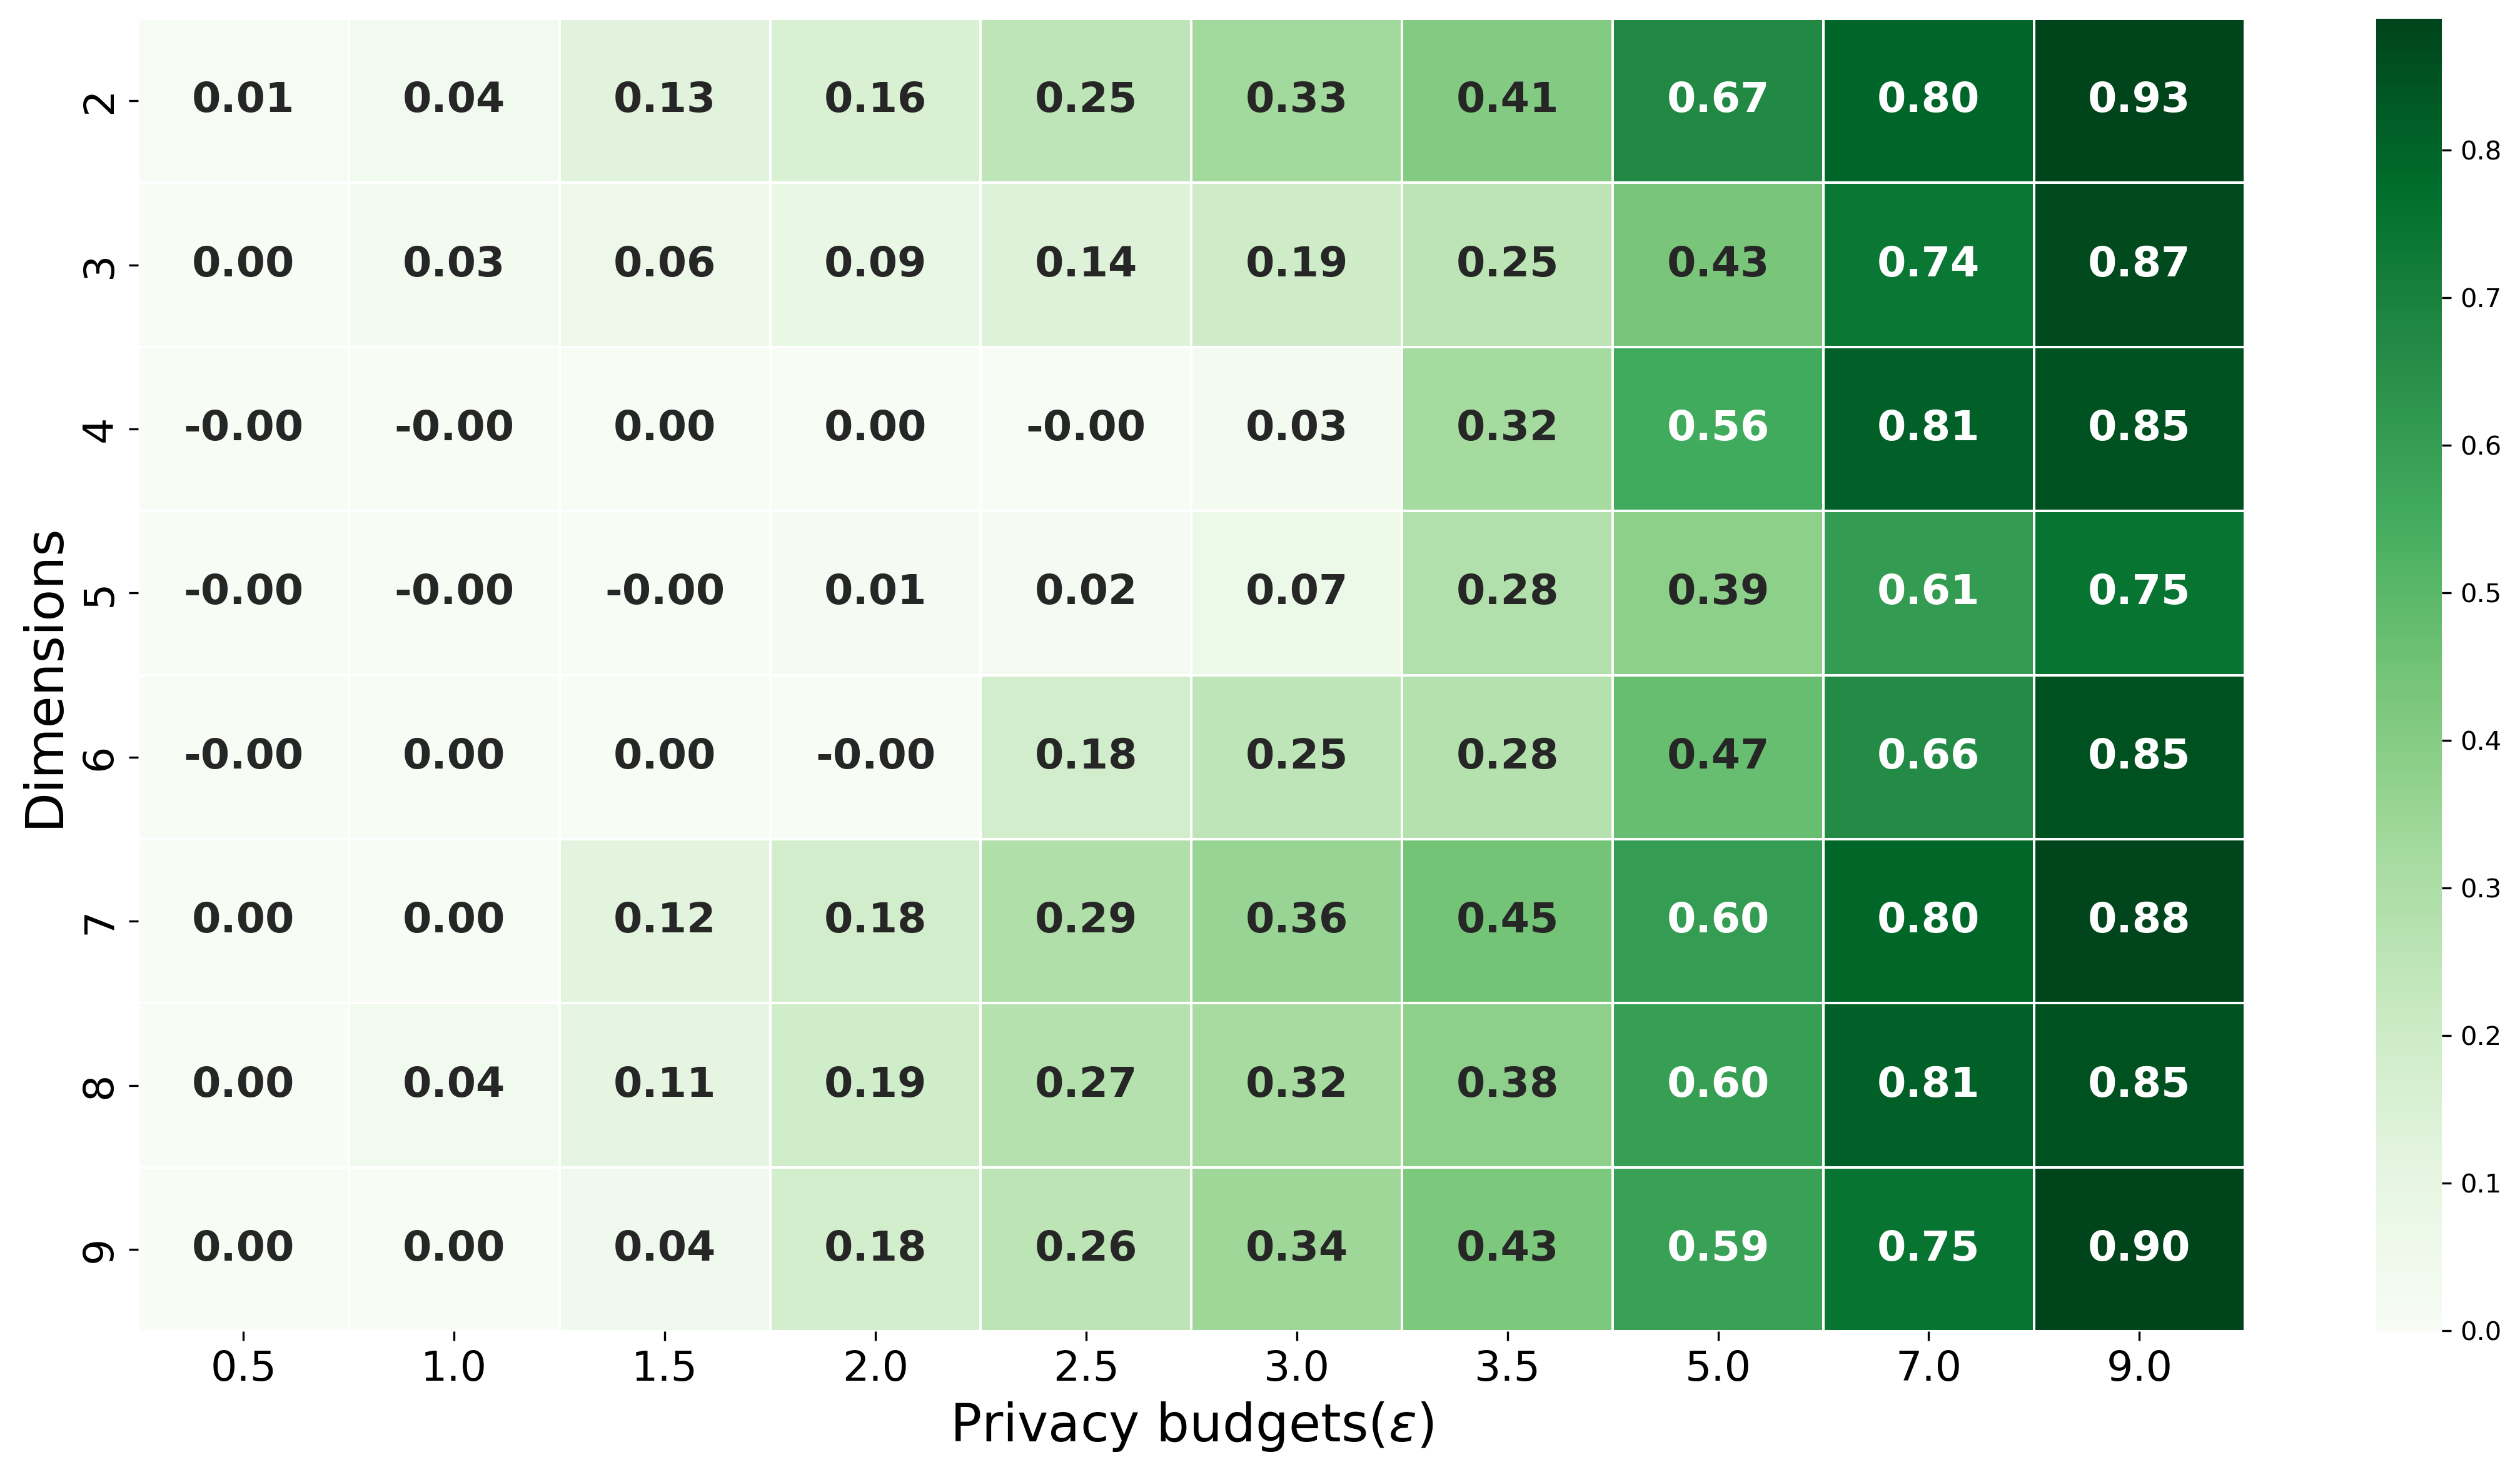
\includegraphics[width=1\textwidth]{Results/nd-laplace/piecewise/heart-dataset/ami.png}
      \label{fig:ami_heart-dataset_comparison_piecewise_2d}
    \end{subfigure}
  \end{subfigure}
\end{figure}
The scores for the heart-dataset are, as expected, in favor of nD-Laplace. We observe the same trend as in the cluster analysis, where nD-Laplace performs well across almost all privacy budgets. The performance of the 3D-Laplace implementation is slightly inferior, a finding that was also noted for the seeds-dataset. The influence of dimensions appears to be somewhat less pronounced than in the seeds-dataset, but from the 5th dimension onward, its impact becomes more significant.

The Piecewise mechanism scores low for privacy budgets between 0.5 and 3. Notably, the scores for 4 and 5 dimensions are considerably lower for these privacy budgets. Beyond that, the number of dimensions has minimal influence on the outcomes, with the privacy budget being the primary determinant.
% \todo[inline]{Why are the 4 / 5 dimensions worse?}
\newpage
\section{Privacy}
The sections below present a heatmap comparison of the nd-Laplace and Piecewise mechanisms.
We employed a heatmap to simultaneously depict the privacy budget (epsilon), the number of dimensions, and a specific metric. The metrics we use for this are the Membership advantage, \gls{tpr} and privacy distance.

On the heatmap, the x-axis represents the privacy budget, while the y-axis illustrates the number of dimensions. Each cell of the heatmap displays the specific metric value. The intensity of the cell's color corresponds to the \gls{ami} score: a darker shade signifies a higher score:
\begin{enumerate}
  \item  For the membership advantage and \gls{tpr}, a lighter cell color (lower value) indicates a better score.
  \item For the privacy distance, the opposite is true; if the cell color is dark (high value), it provides more distance and thus more privacy.
\end{enumerate}
%The images below display bar plots for the membership advantage and TPR of membership inference attacks as described in the methodology.
%We use the same color scheme in the previous section to display the different mechanisms.
%In addition, a red line was drawn to indicate the baseline TPR (the non-private dataset's TPR). \newline
\newpage
\subsection{Seeds dataset}
\begin{figure}[H]
  \centering
  \begin{subfigure}[b]{0.75\textwidth}
    \begin{subfigure}[c]{1\textwidth}
      \caption{\textbf{Heatmap showing membership advantage for the nD-Laplace mechanism, per privacy budget \& dimension for seeds-dataset.}}
      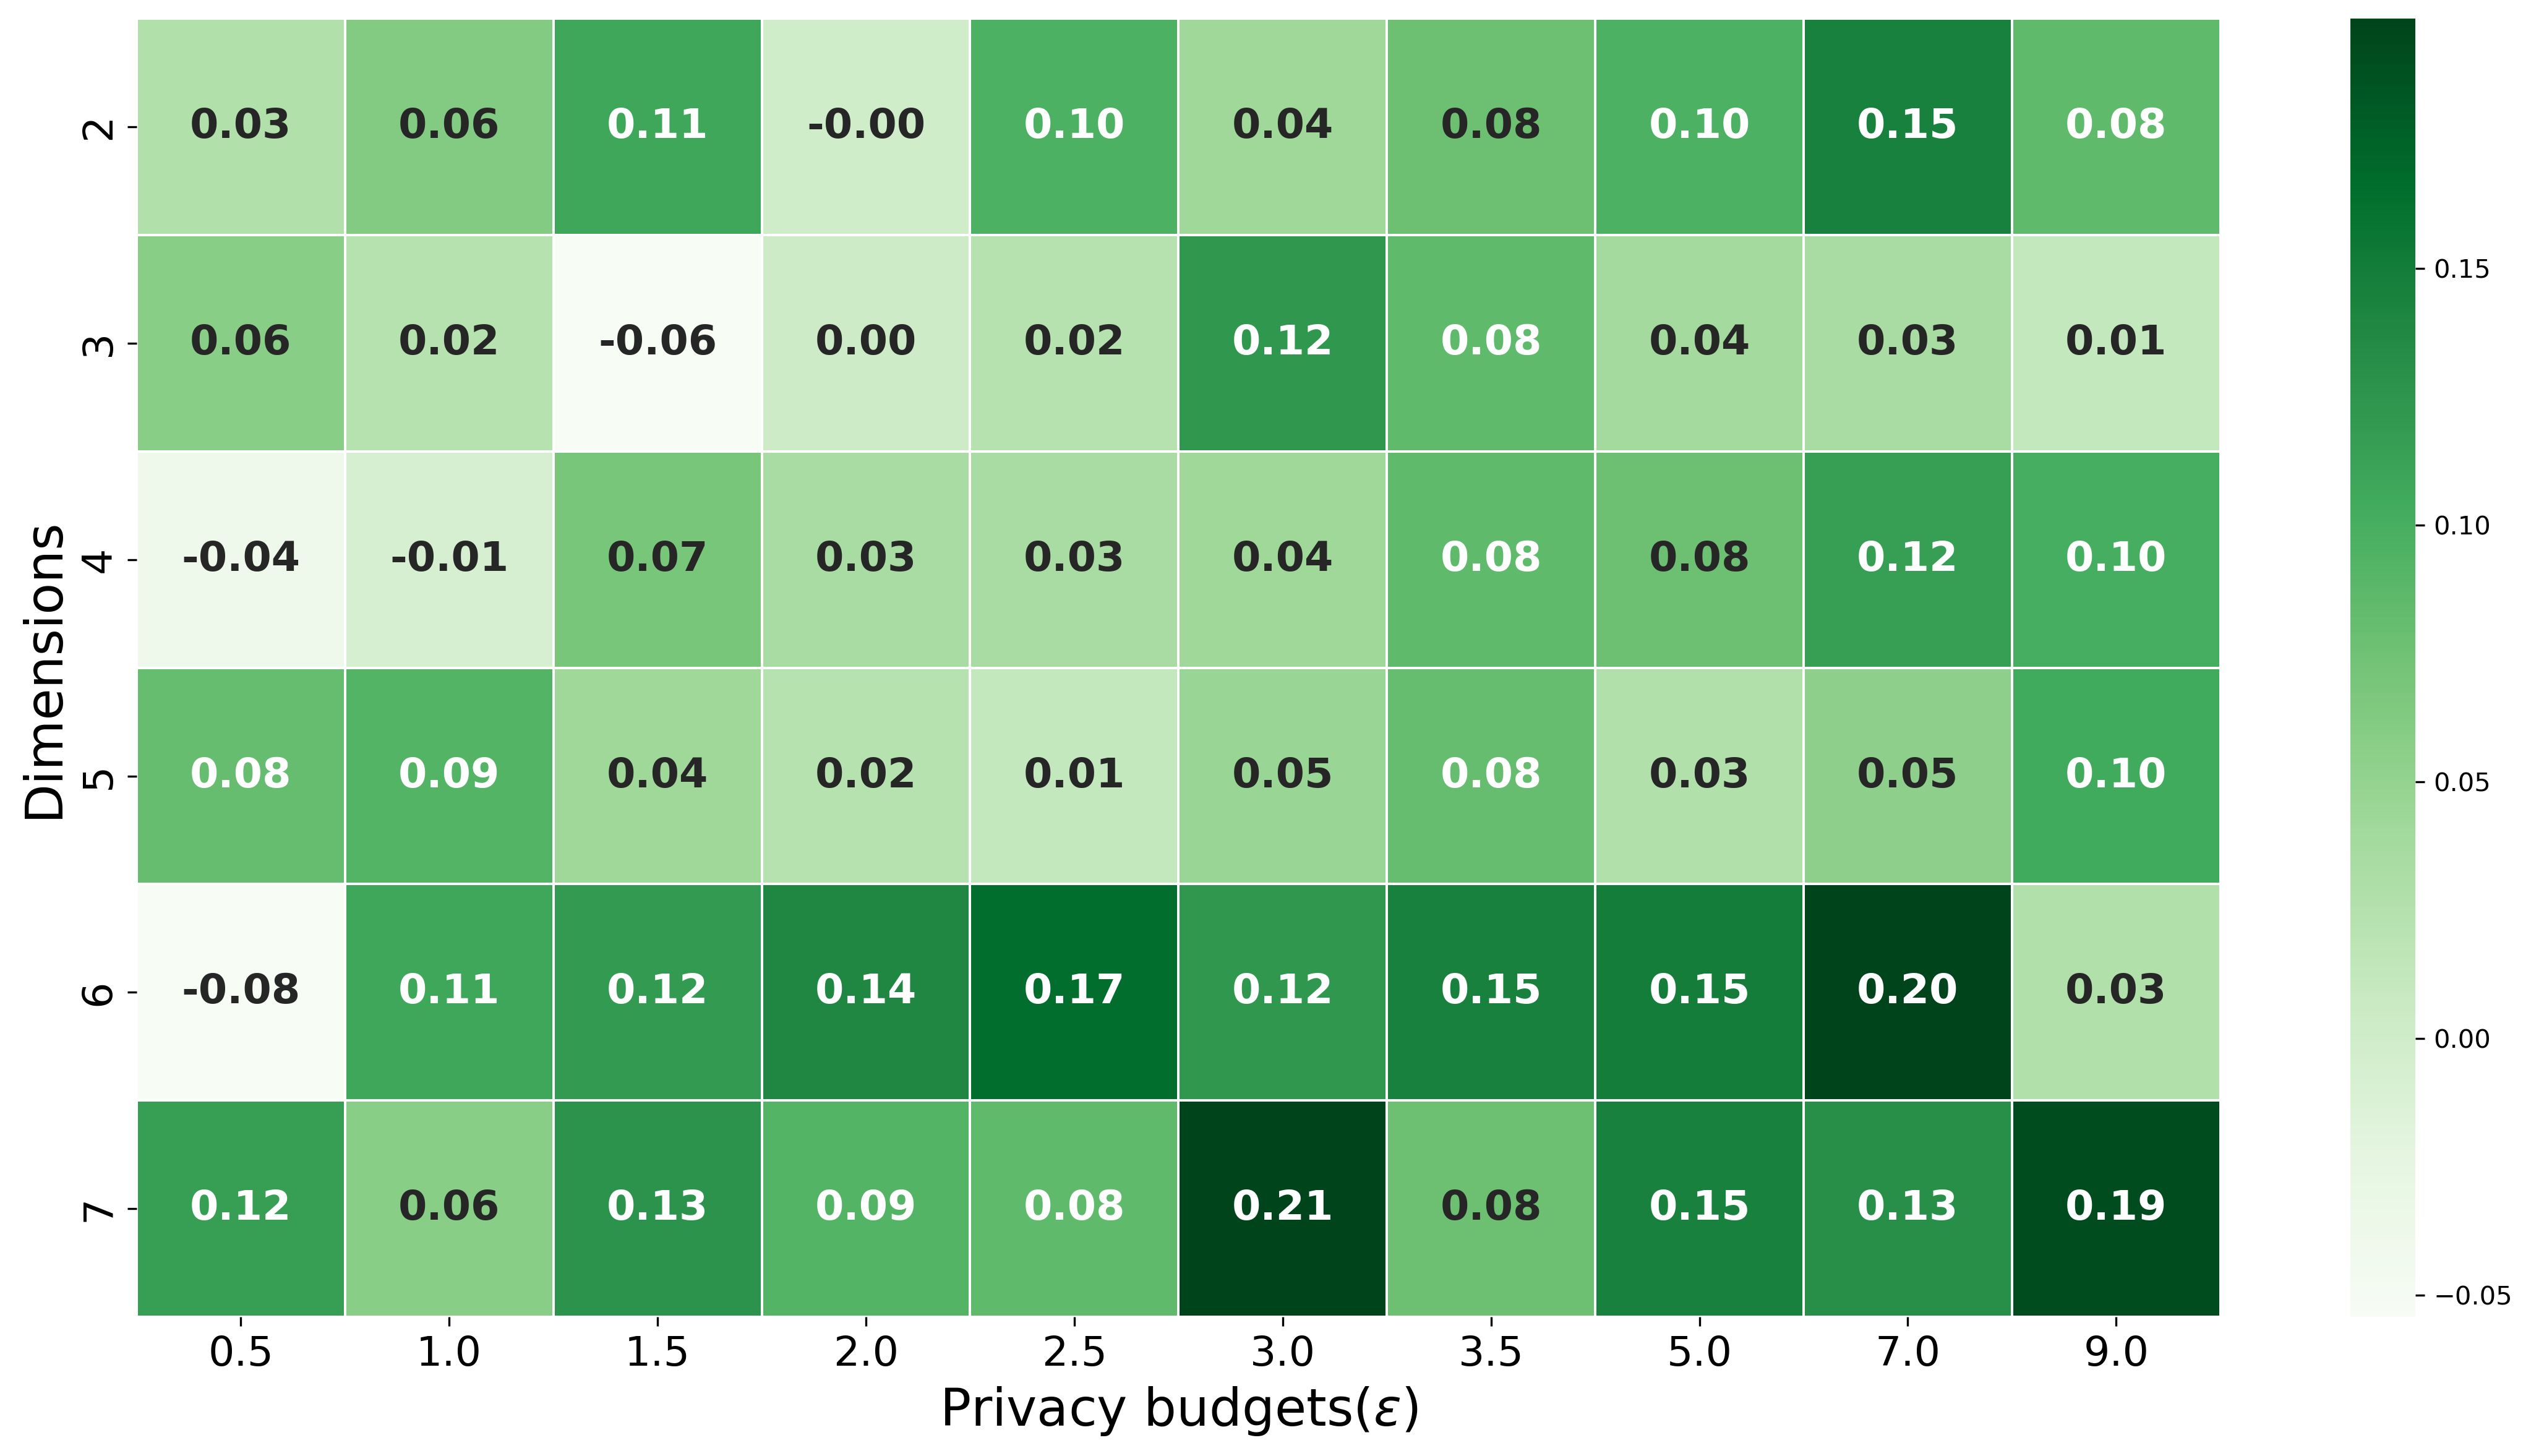
\includegraphics[width=1\textwidth]{Results/nd-laplace/nd-Laplace/seeds-dataset/attack_adv.png}
      \label{fig:privacy_seeds-dataset_adversial_advantage_kd-laplace}
    \end{subfigure}
    \vfill % vertical space

    \begin{subfigure}[c]{1\textwidth}
      \caption{\textbf{Heatmap showing adversary advantage for the Piecewise mechanism, per privacy budget \& dimension for seeds-dataset.}}
      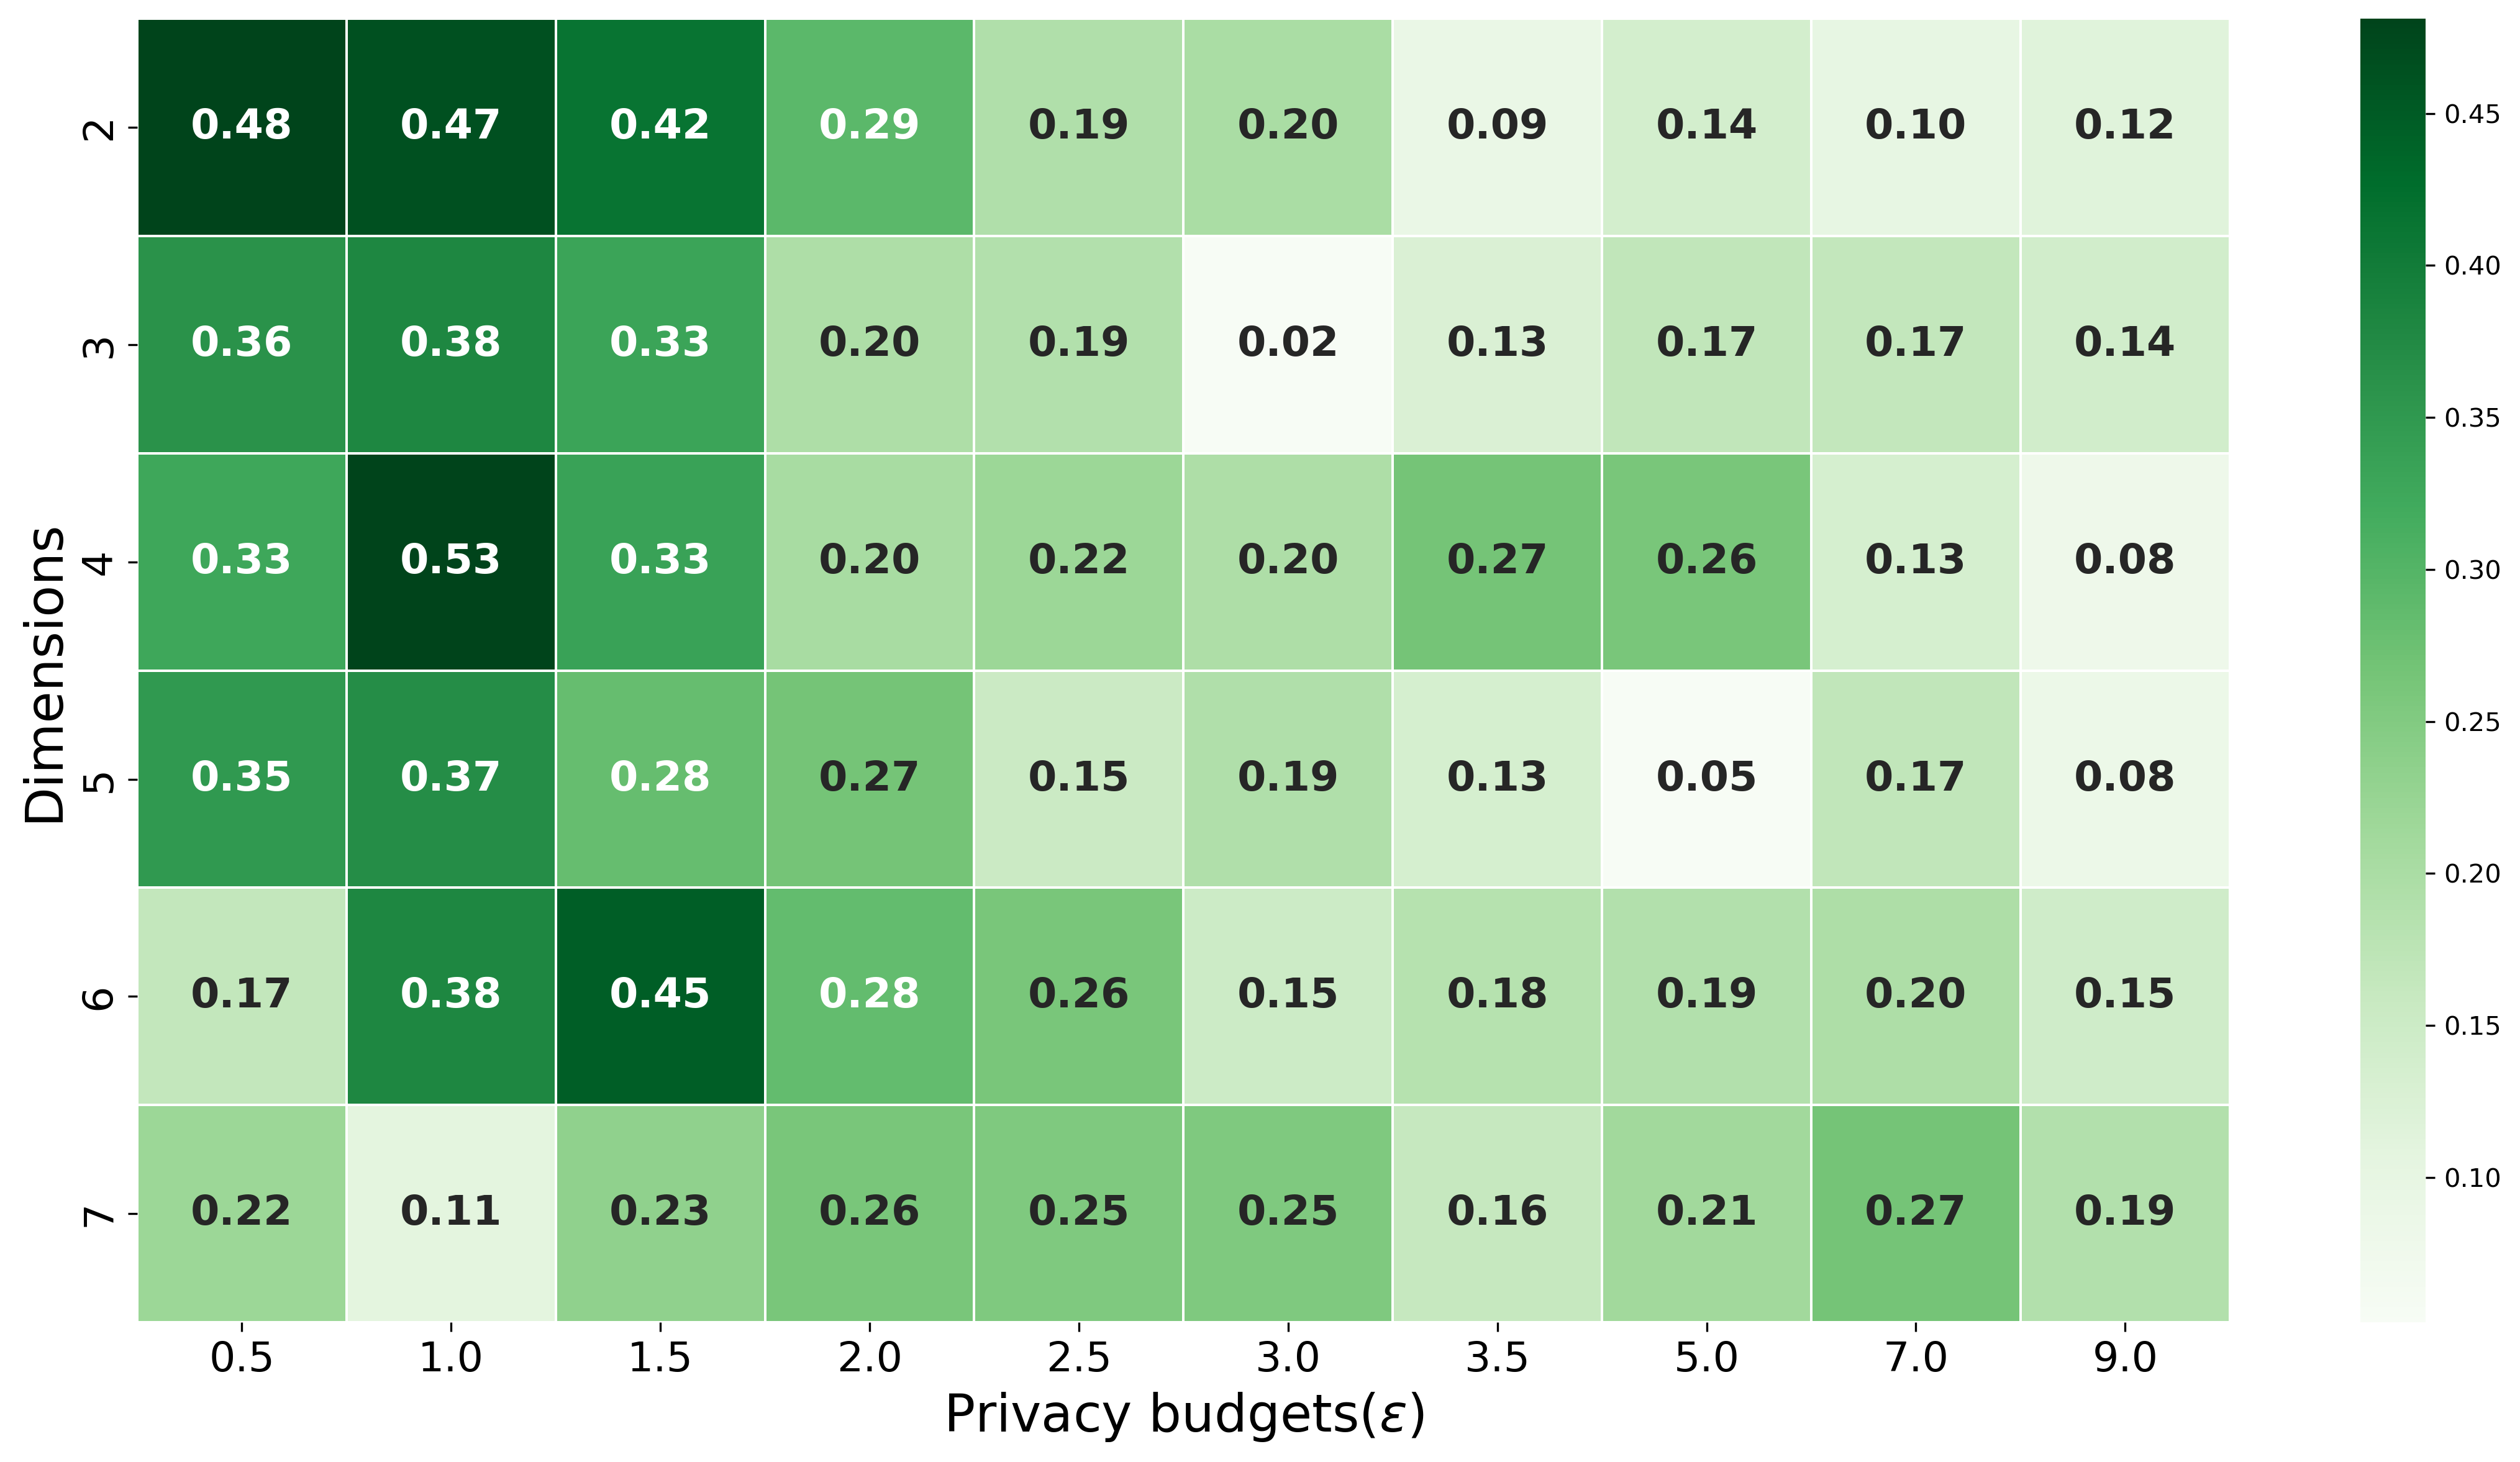
\includegraphics[width=1\textwidth]{Results/nd-laplace/piecewise/seeds-dataset/attack_adv.png}
      \label{fig:privacy_seeds-dataset_adversial_advantage_piecewise}
    \end{subfigure}
  \end{subfigure}
\end{figure}
When evaluating the mechanisms, it's evident that nD-Laplace consistently achieves higher scores for epsilon values, particularly in dimensions 6 and 7. This suggests that the number of dimensions significantly influences the results to a certain degree. As privacy budgets rise, so does the adversary advantage. However, there are anomalies in the nD-Laplace results, such as the 0.03 advantage for epsilon 9, which deviates from the expected range of 0.15 to 0.20. In contrast, the Piecewise mechanism displays a clear color gradient that darkens from left to right, aligning with expectations: the membership advantage tends to increase as the privacy budget diminishes. Notably, the Piecewise mechanism introduces substantial noise for privacy budgets between 0.5 and 1.5, attributed to the unbounded noise that surpasses the original domain $X$. This observation aligns with the \gls{ami} results from the 2-dimensional seeds-dataset, where Piecewise registered a score of 0 for these specific privacy budgets.

The membership advantage provides valuable insights into the privacy attributes of the Piecewise mechanism. However, given the inconsistent outcomes associated with nD-Laplace, a more refined metric is warranted. As such, we will delve into the \gls{tpr} to offer a clearer depiction of the mechanisms' behaviors (details on the subsequent page).\newpage
\begin{figure}[H]
  \centering
  \begin{subfigure}[b]{0.75\textwidth}
    \begin{subfigure}[c]{1\textwidth}
      \caption{\textbf{Heatmap TPR for the nD-Laplace mechanism, per privacy budget \& dimension for seeds-dataset.}}
      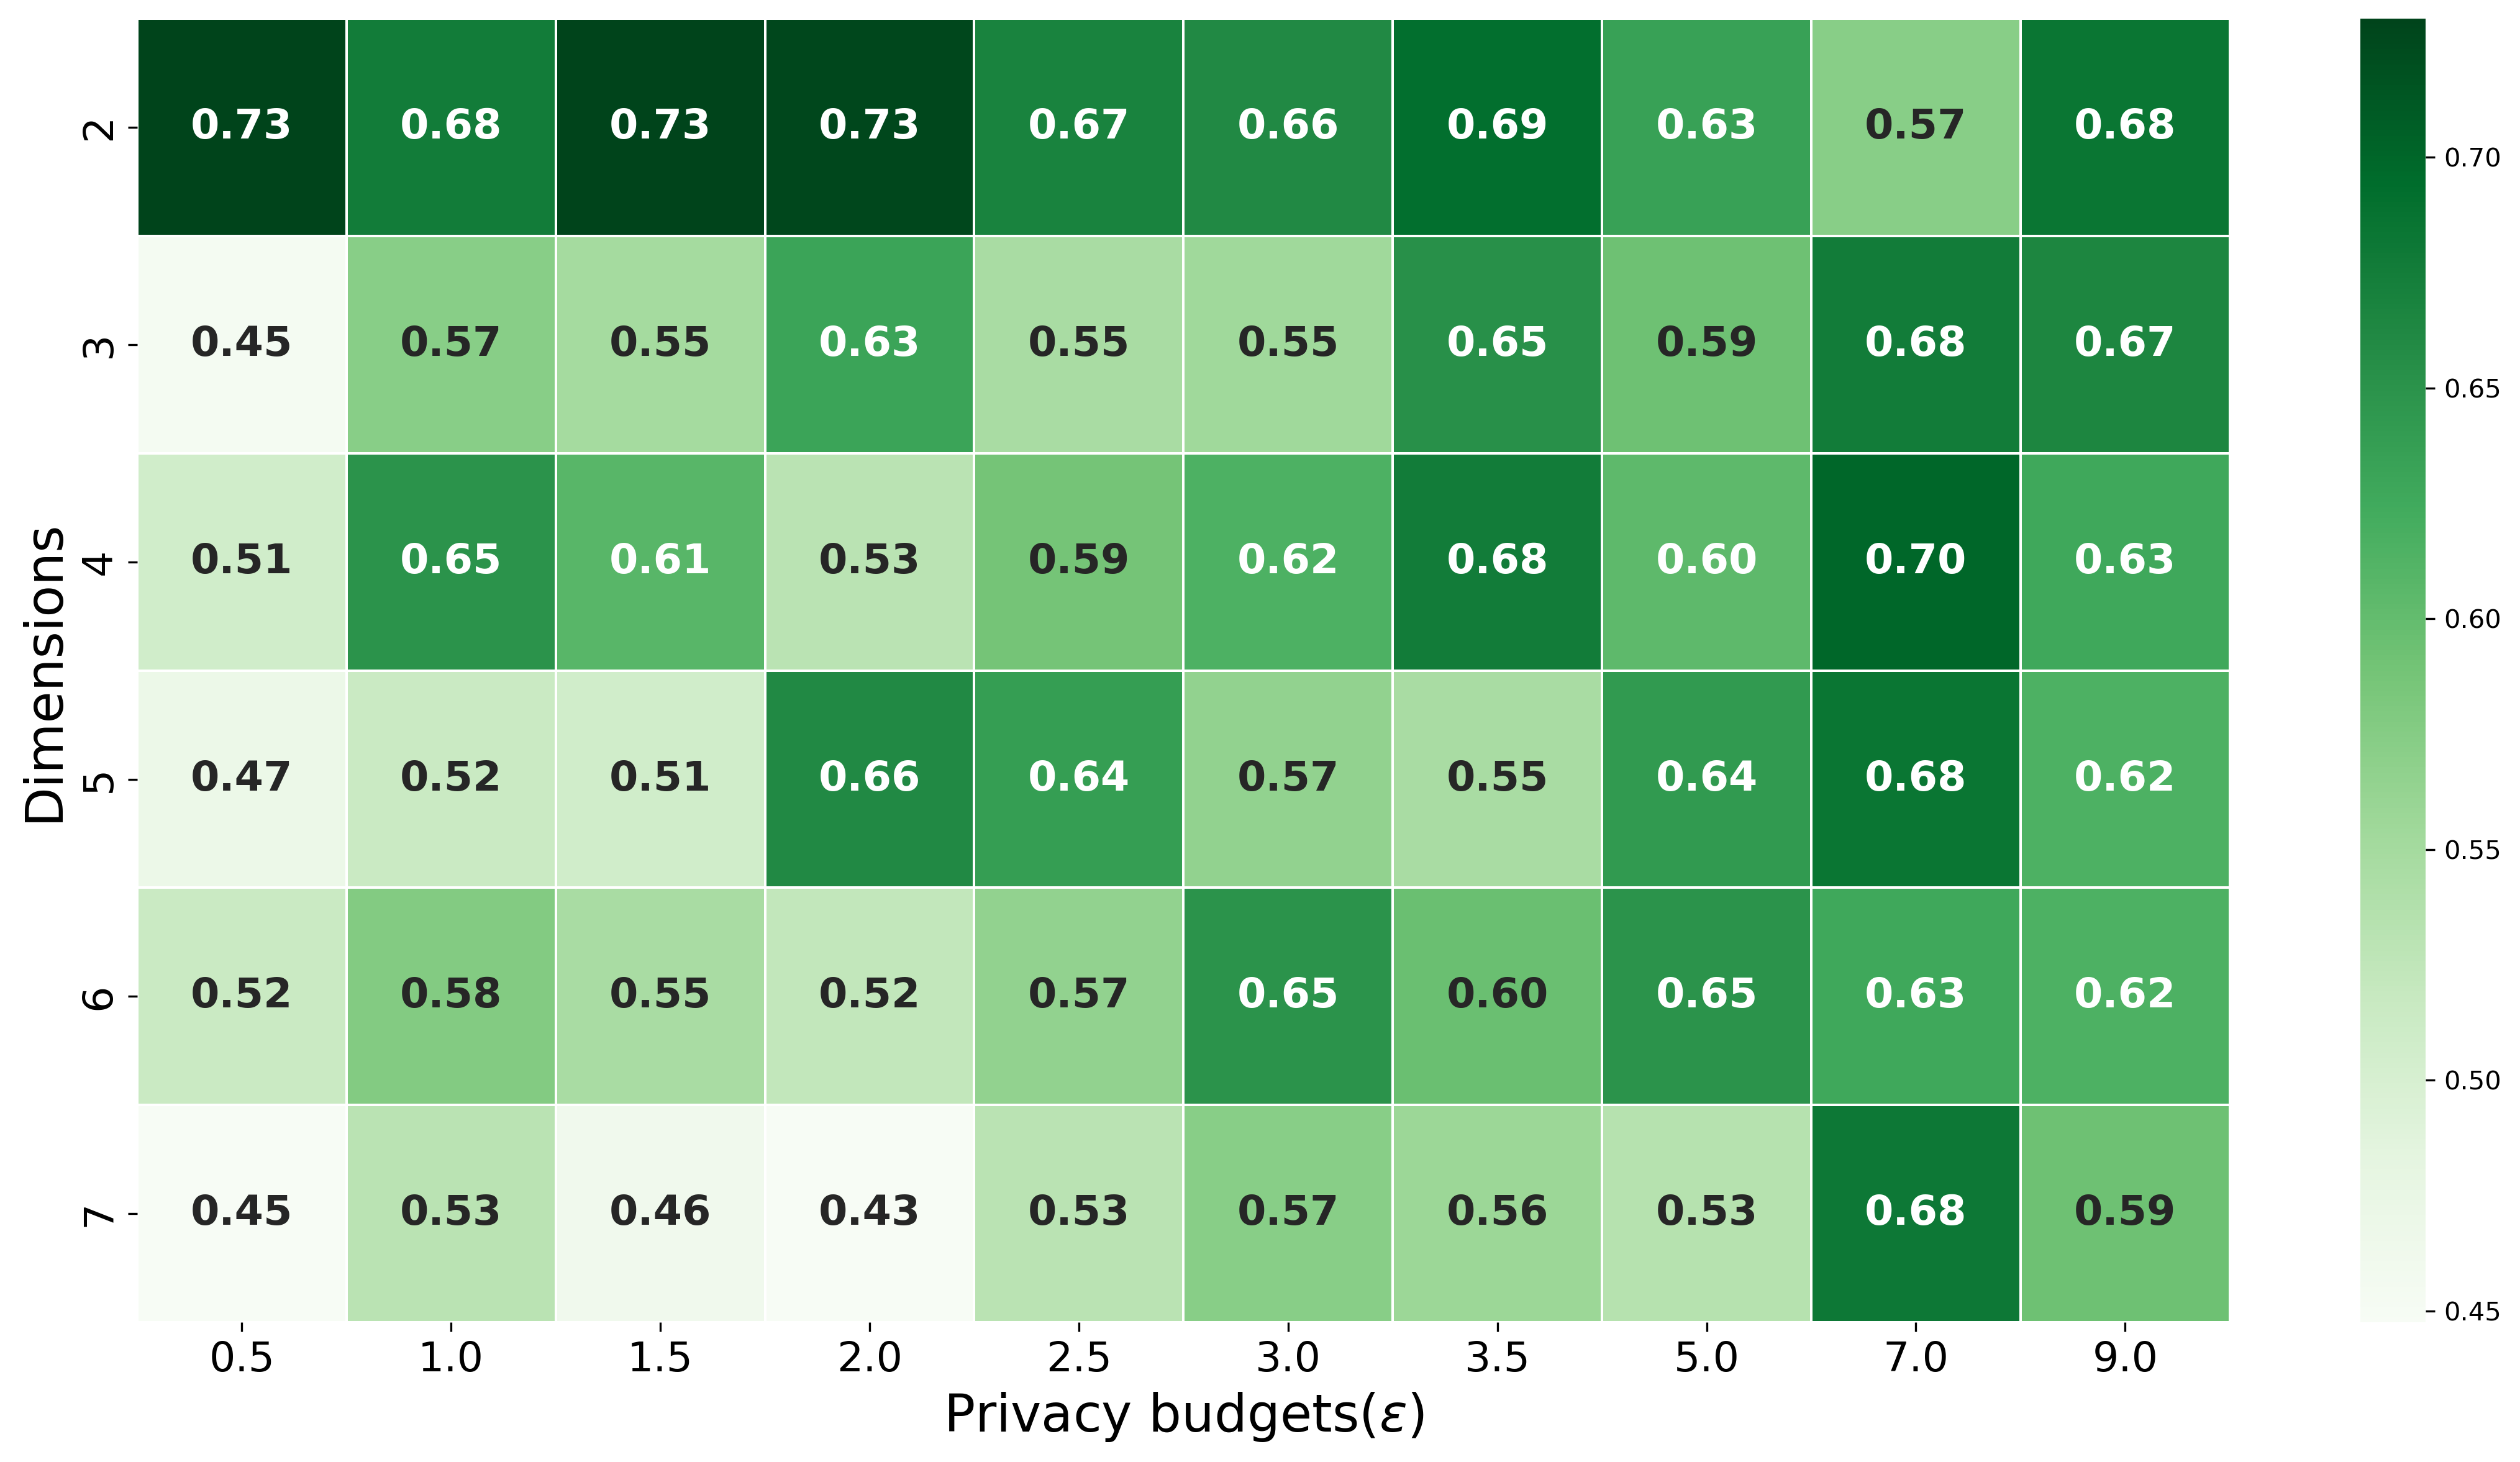
\includegraphics[width=1\textwidth]{Results/nd-laplace/nd-Laplace/seeds-dataset/tpr.png}
      \label{fig:privacy_tpr_seeds-dataset_adversial_advantage_kd-laplace}
    \end{subfigure}
    \vfill % vertical space
    \begin{subfigure}[c]{1\textwidth}
      \caption{\textbf{Heatmap TPR for the Piecewise mechanism, per privacy budget \& dimension for seeds-dataset.}}
      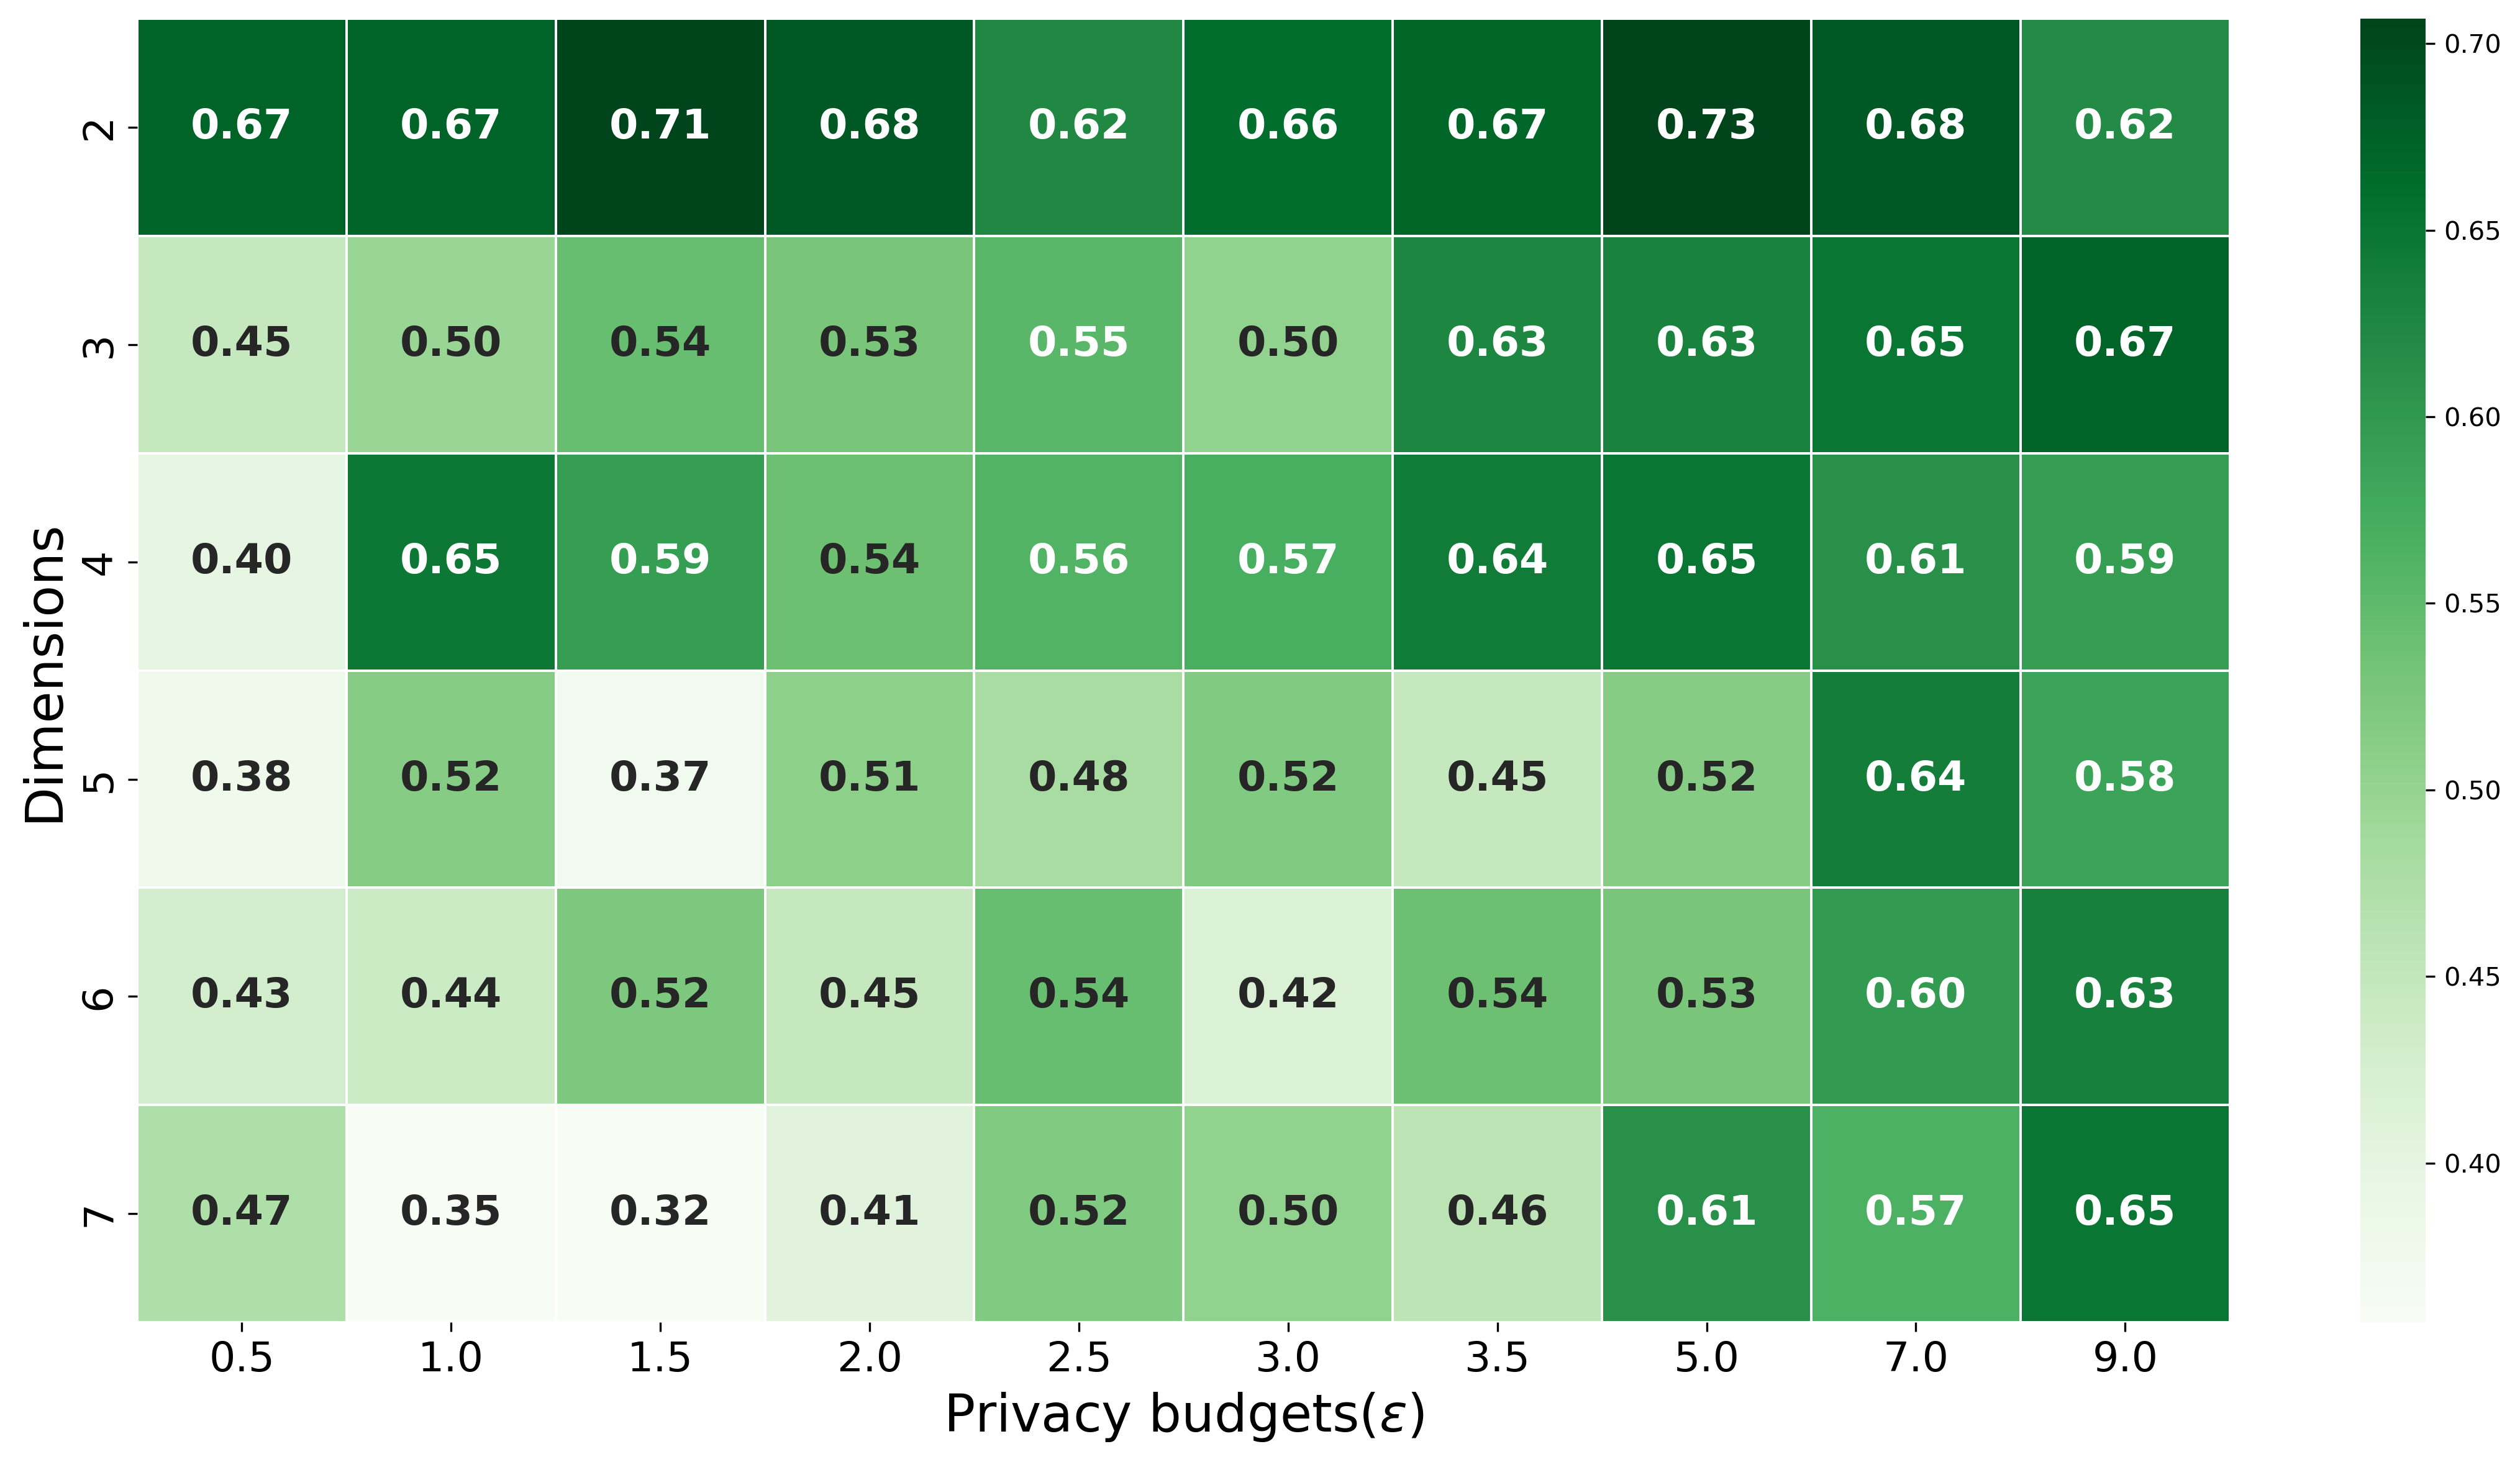
\includegraphics[width=1\textwidth]{Results/nd-laplace/piecewise/seeds-dataset/tpr.png}
      \label{fig:privacy_tpr_seeds-dataset_adversial_advantage_piecewise}
    \end{subfigure}
  \end{subfigure}
\end{figure}
The top result displays a more stable outcome for the nD-Laplace mechanism. There's a clear progression from light to dark as the privacy budget increases. The number of dimensions does not seem to have a significant influence; however, it's noteworthy that the 2-dimensional data scores higher for lower privacy budgets. The Piecewise mechanism exhibits a similar pattern, but there's a peculiar observation in the bottom left corner. The low membership advantages (ranging from -0.50 to 0.70) are not as promising as they initially appear. Given that the \gls{tpr} is quite high, it highlights the limitations of the membership advantage metric. A high \gls{tpr} (and consequently a low \gls{fpr}) can distort the actual representation.

\newpage
\subsection{Heart dataset}
\begin{figure}[H]
  \centering
  \begin{subfigure}[b]{0.75\textwidth}
    \begin{subfigure}[c]{1\textwidth}
      \caption{\textbf{Heatmap showing adversary advantage for the nD-Laplace mechanism, per privacy budget \& dimension for heart-dataset.}}
      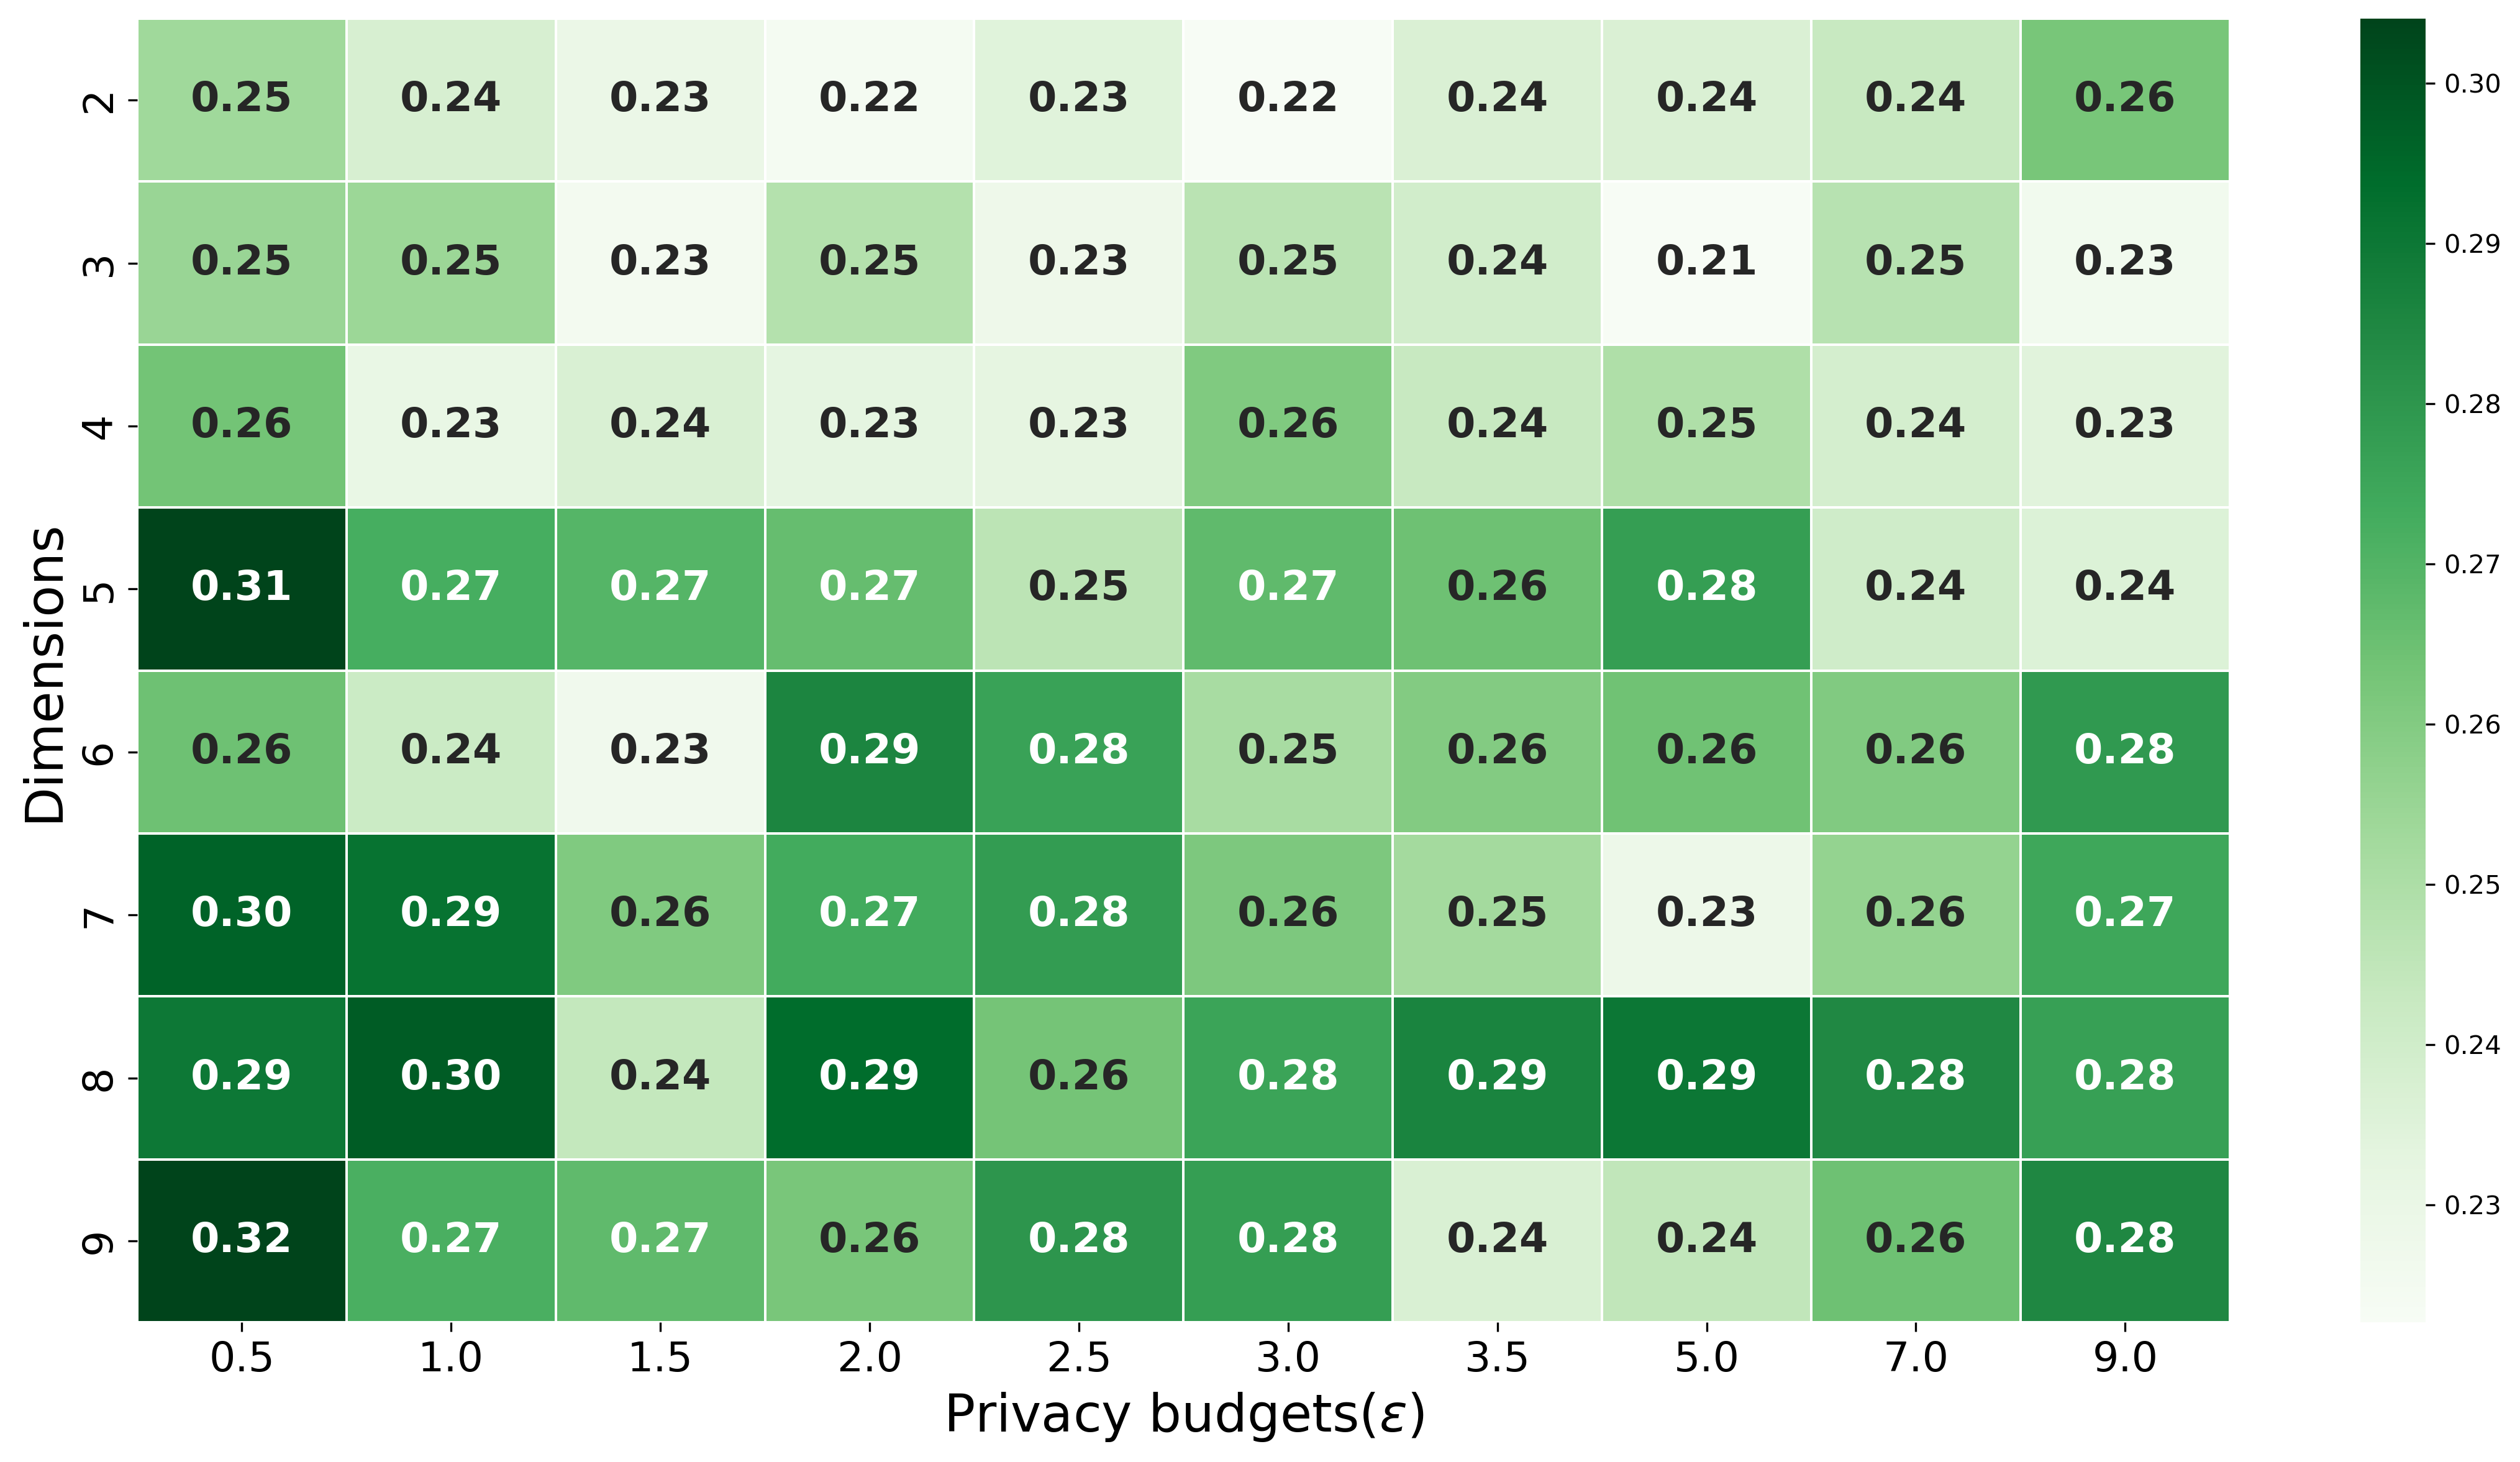
\includegraphics[width=1\textwidth]{Results/nd-laplace/nd-Laplace/heart-dataset/attack_adv.png}
      \label{fig:privacy_heart-dataset_adversial_advantage_kd-laplace}
    \end{subfigure}
    \vfill % vertical space

    \begin{subfigure}[c]{1\textwidth}
      \caption{\textbf{Heatmap showing adversary advantage for the Piecewise mechanism, per privacy budget \& dimension for heart-dataset.}}
      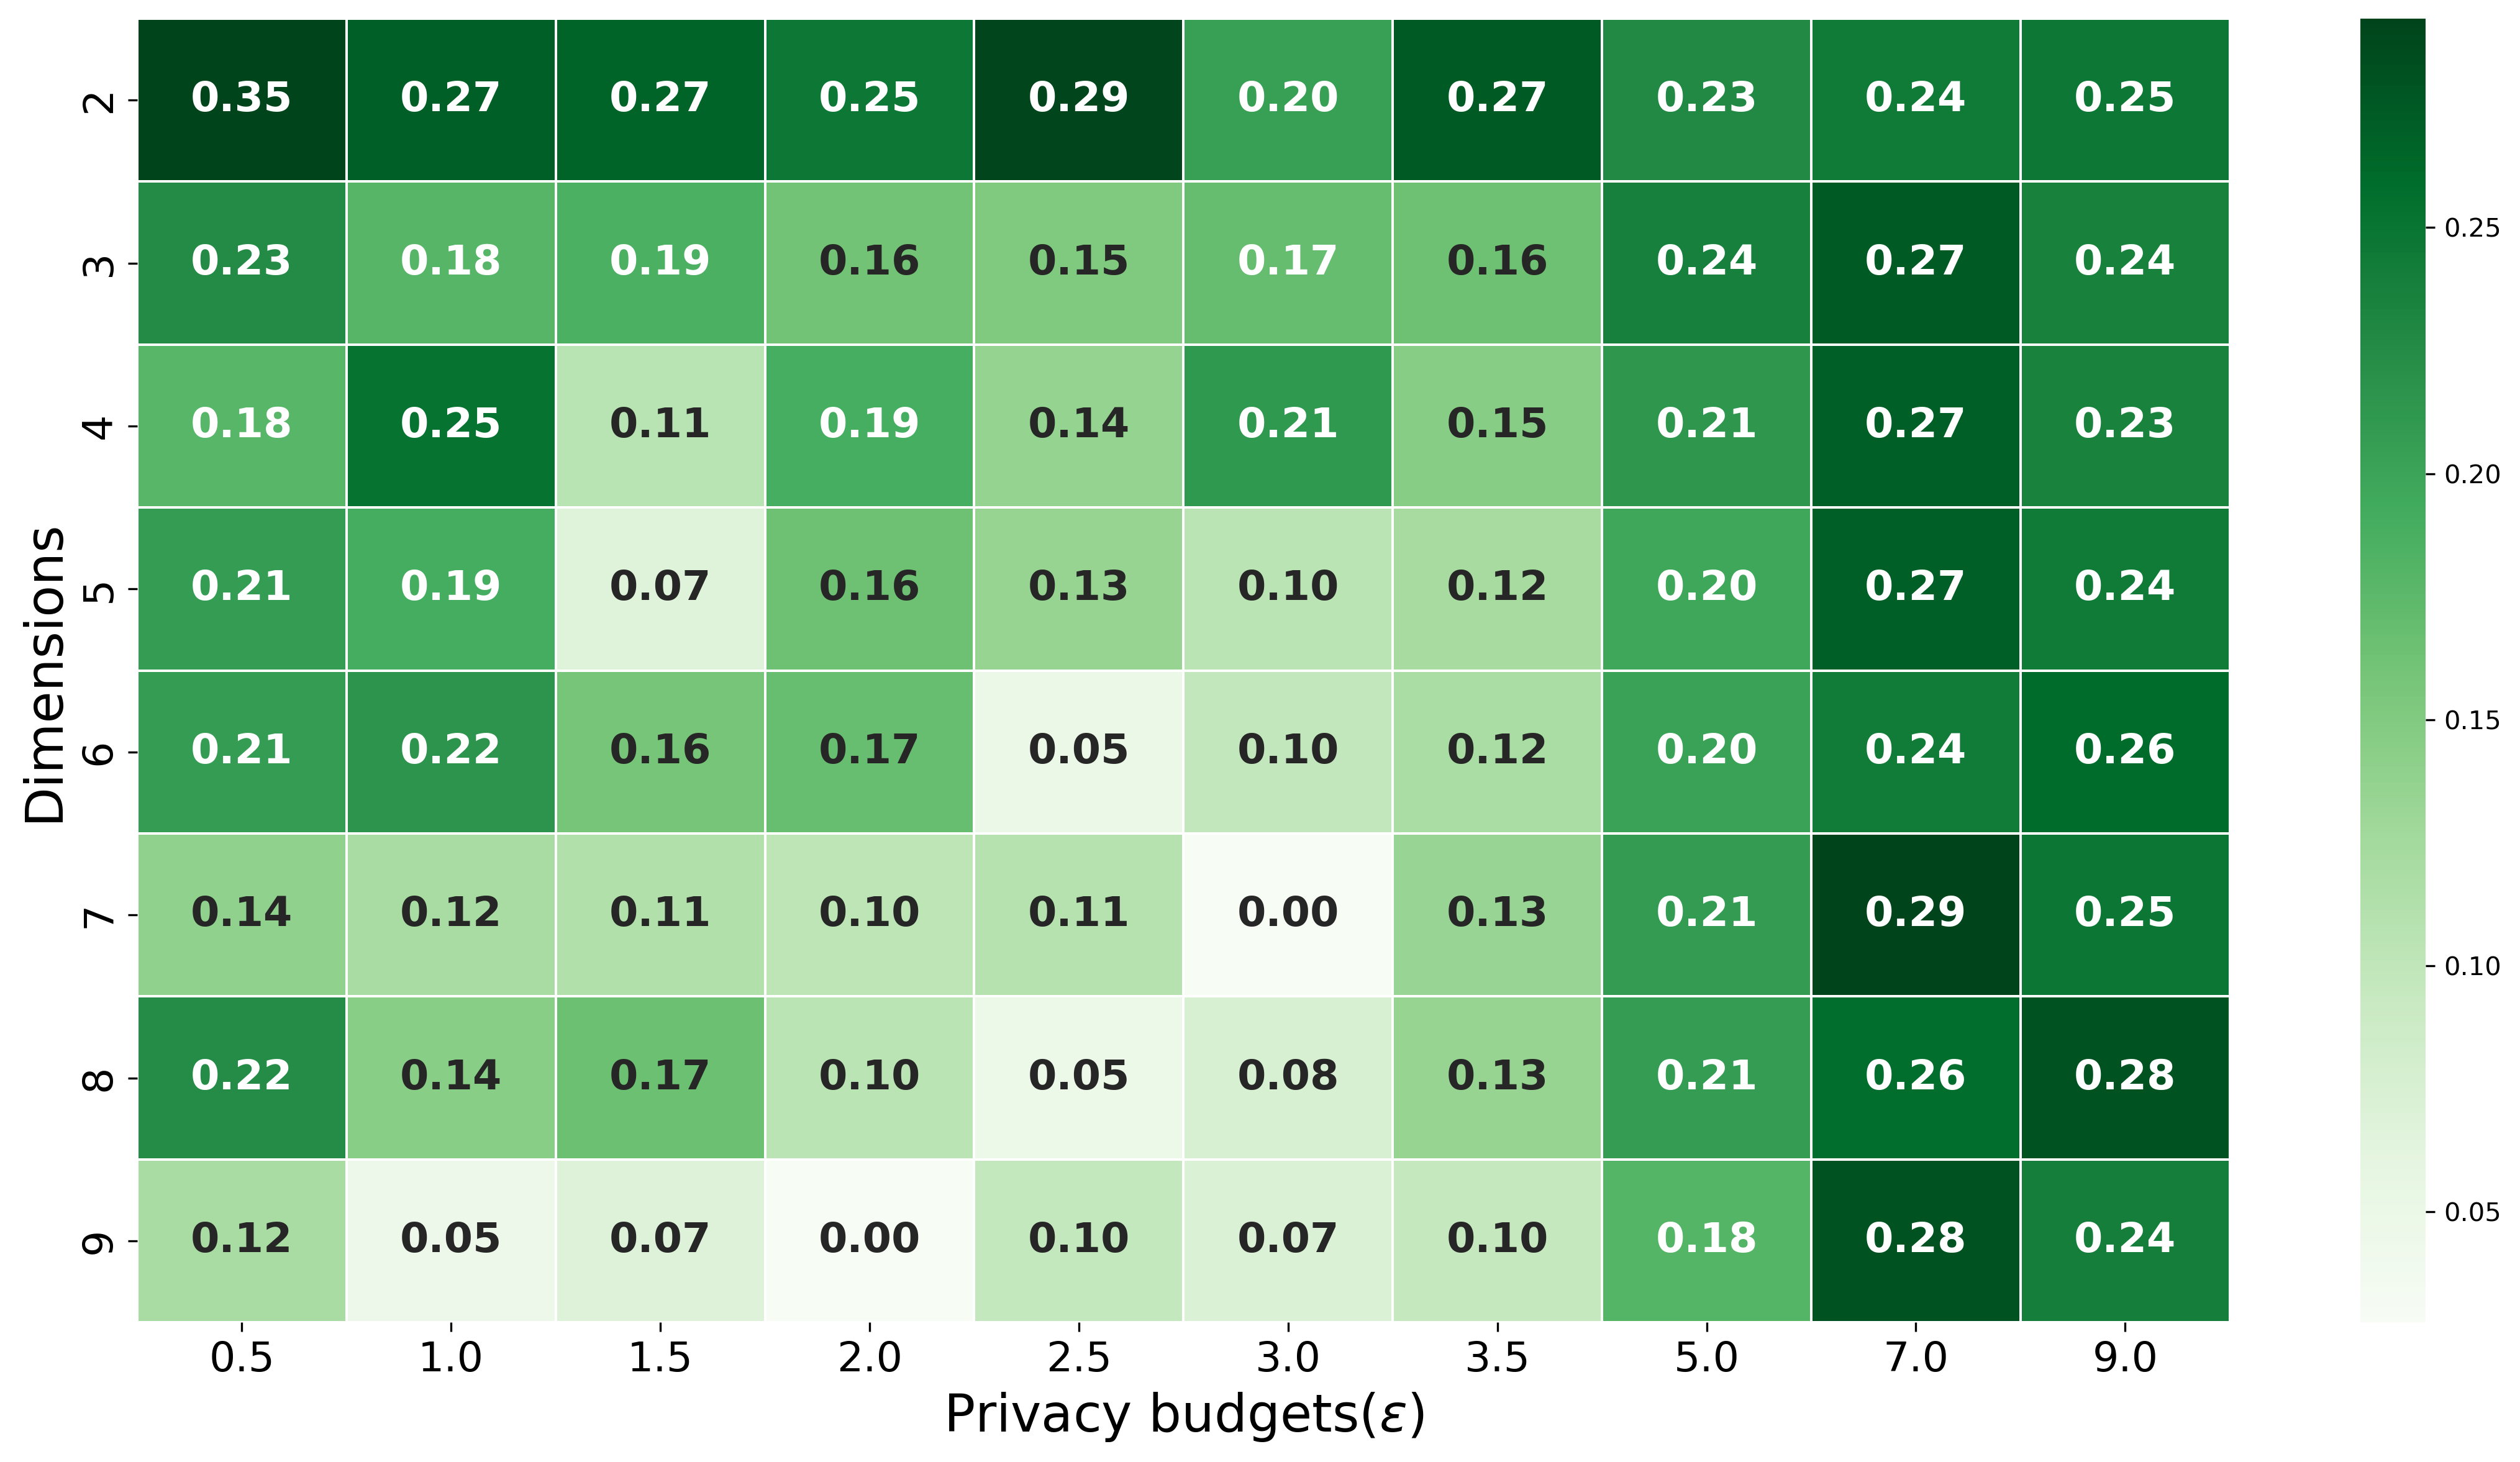
\includegraphics[width=1\textwidth]{Results/nd-laplace/piecewise/heart-dataset/attack_adv.png}
      \label{fig:privacy_heart-dataset_adversial_advantage_piecewise}
    \end{subfigure}
  \end{subfigure}
\end{figure}
For the nD-Laplace mechanism, minimal variation is observed across different privacy budgets and dimensions, aligning with the consistent \gls{ami} scores. While there's a slight dip in membership advantage for dimensions greater than 5, the results remain somewhat inconsistent, similar to those from the seeds-dataset.

In contrast, the Piecewise mechanism displays a distinct pattern. The membership advantage peaks for 2-dimensional data and diminishes as the number of dimensions increases. The higher privacy budgets appear to compromise privacy, which aligns with expectations for increased privacy budgets.

While the adversary advantage in the heatmaps for the Piecewise mechanism logically increases from left to right, the nD-Laplace mechanism still presents some inconsistencies. To gain a clearer understanding, we will delve into the \gls{tpr} on the subsequent page.
\newpage
\begin{figure}[H]
  \centering
  \begin{subfigure}[b]{0.75\textwidth}
    \begin{subfigure}[c]{1\textwidth}
      \caption{\textbf{Heatmap TPR for the nD-Laplace mechanism, per privacy budget \& dimension for heart-dataset.}}
      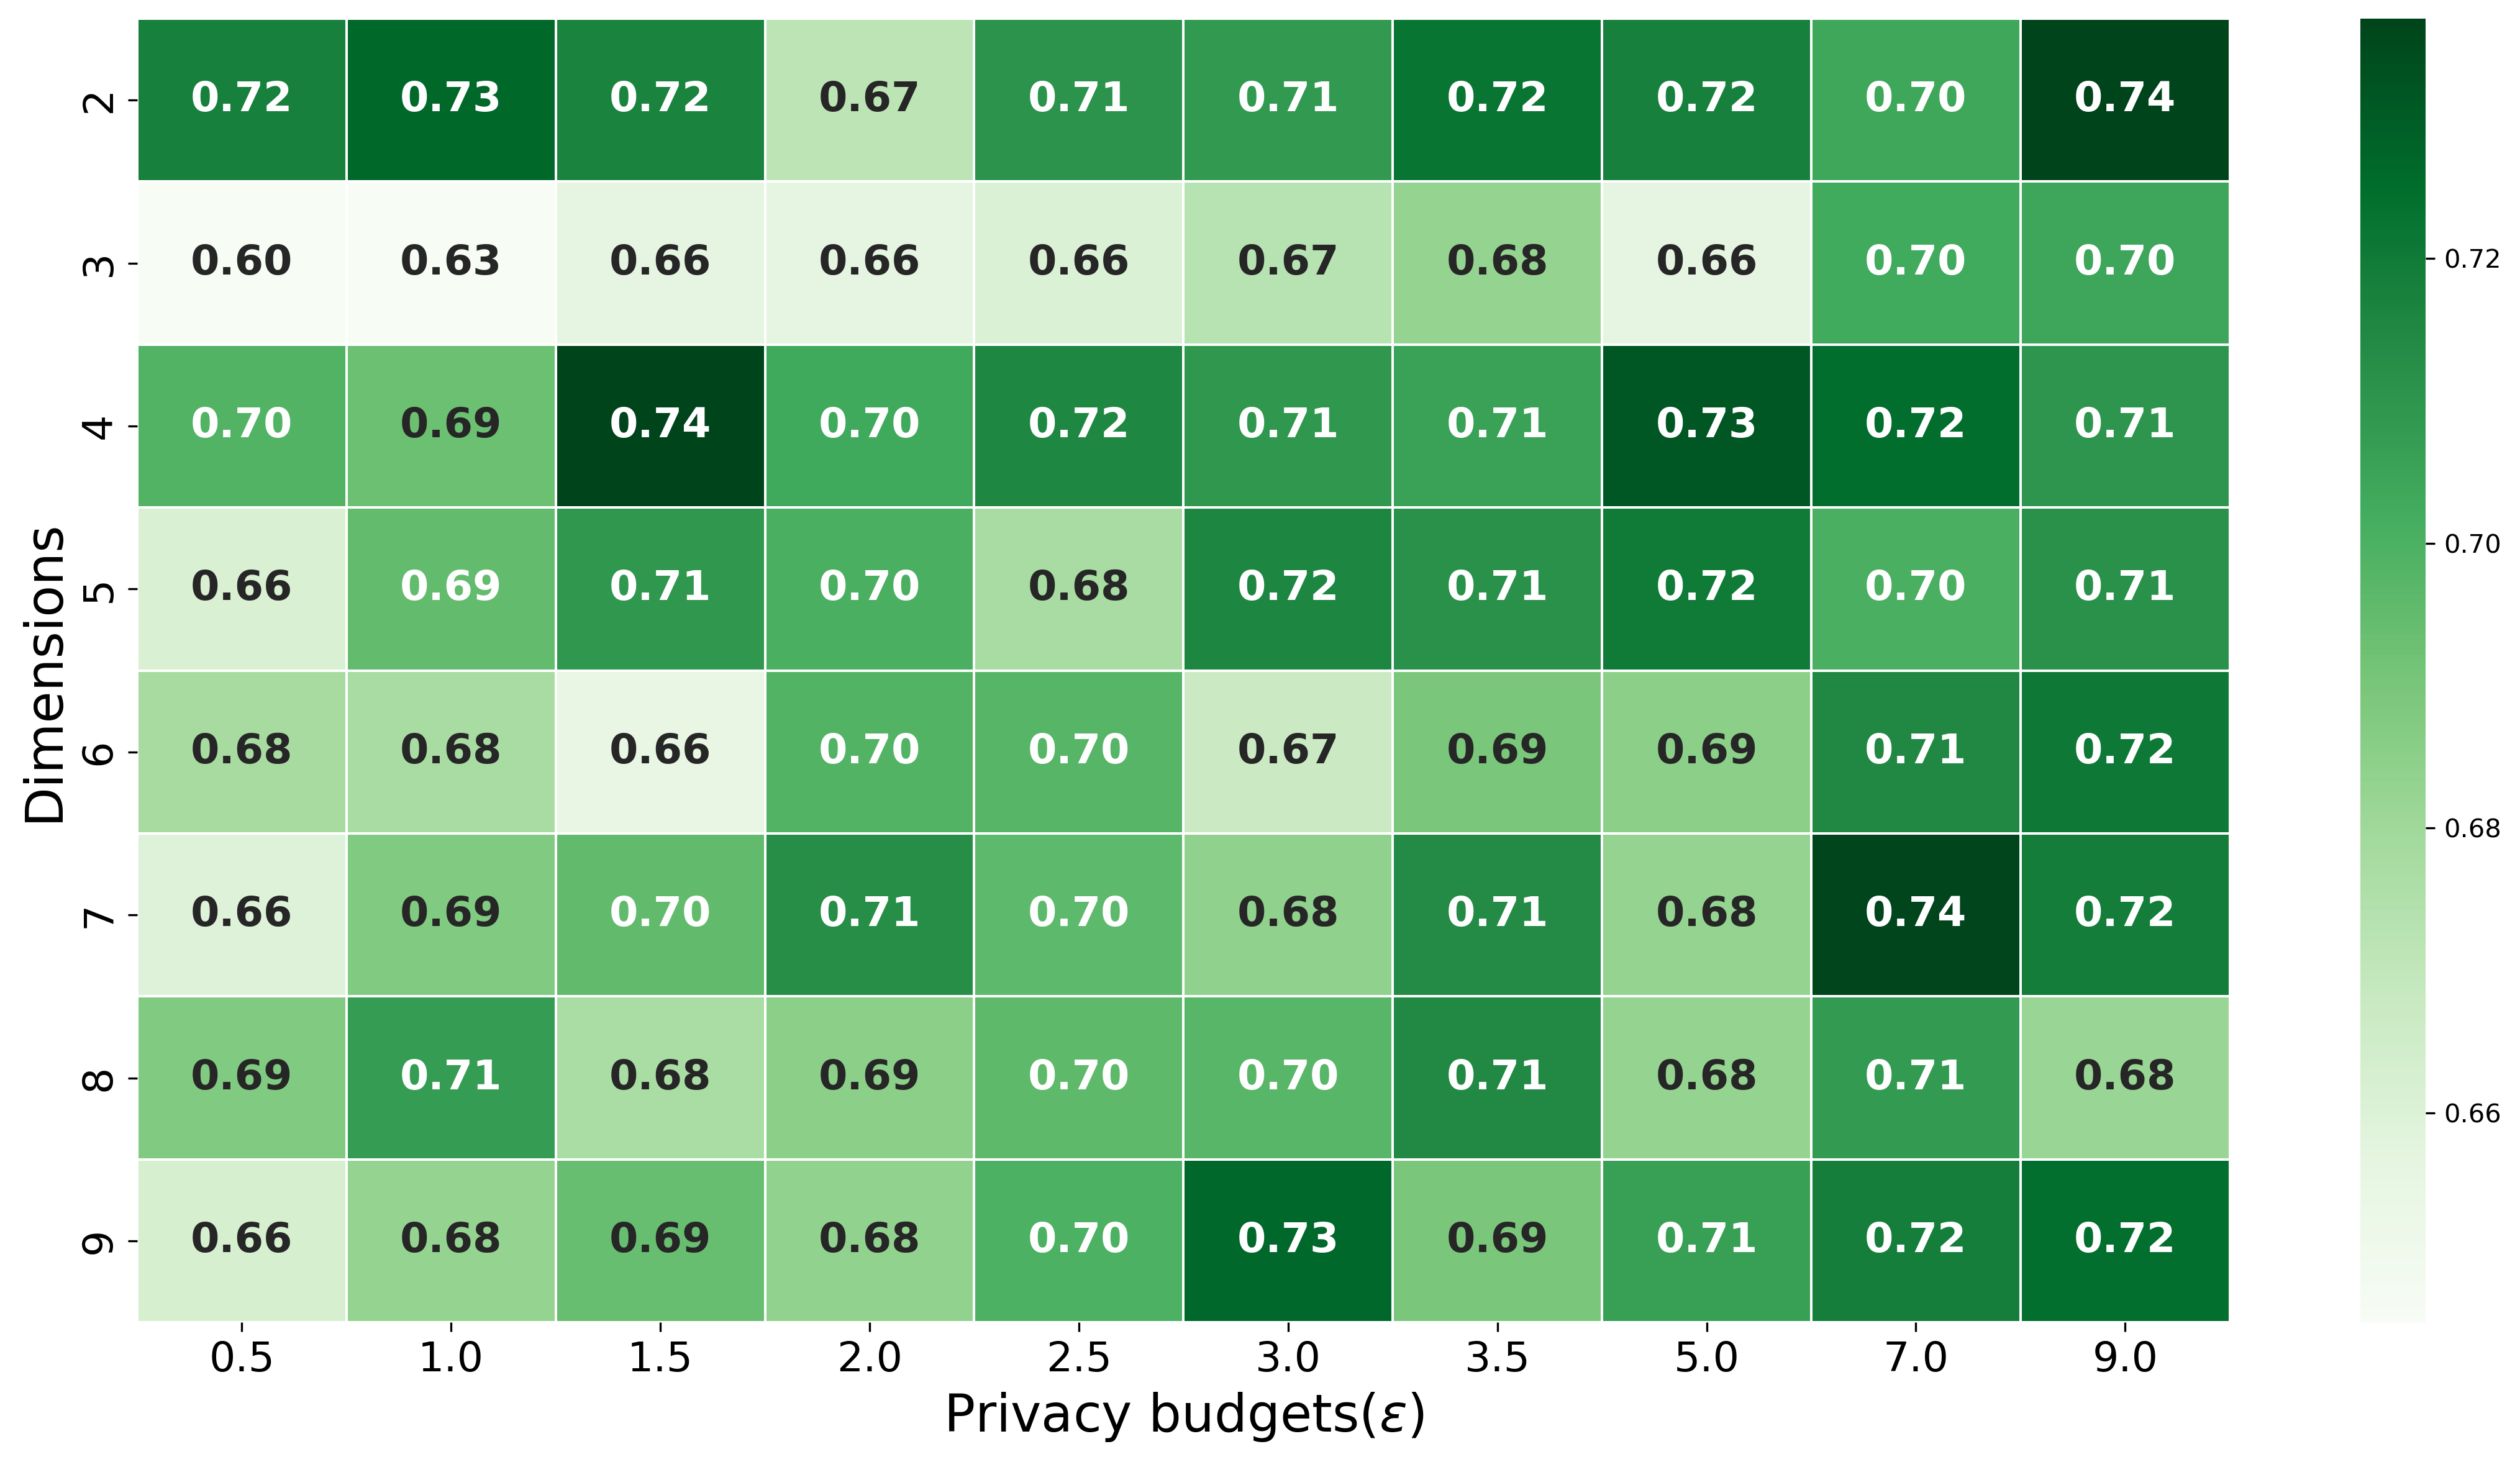
\includegraphics[width=1\textwidth]{Results/nd-laplace/nd-Laplace/heart-dataset/tpr.png}
      \label{fig:privacy_tpr_heart-dataset_adversial_advantage_kd-laplace}
    \end{subfigure}
    \vfill % vertical space

    \begin{subfigure}[c]{1\textwidth}
      \caption{\textbf{Heatmap TPR for the Piecewise mechanism, per privacy budget \& dimension for heart-dataset.}}
      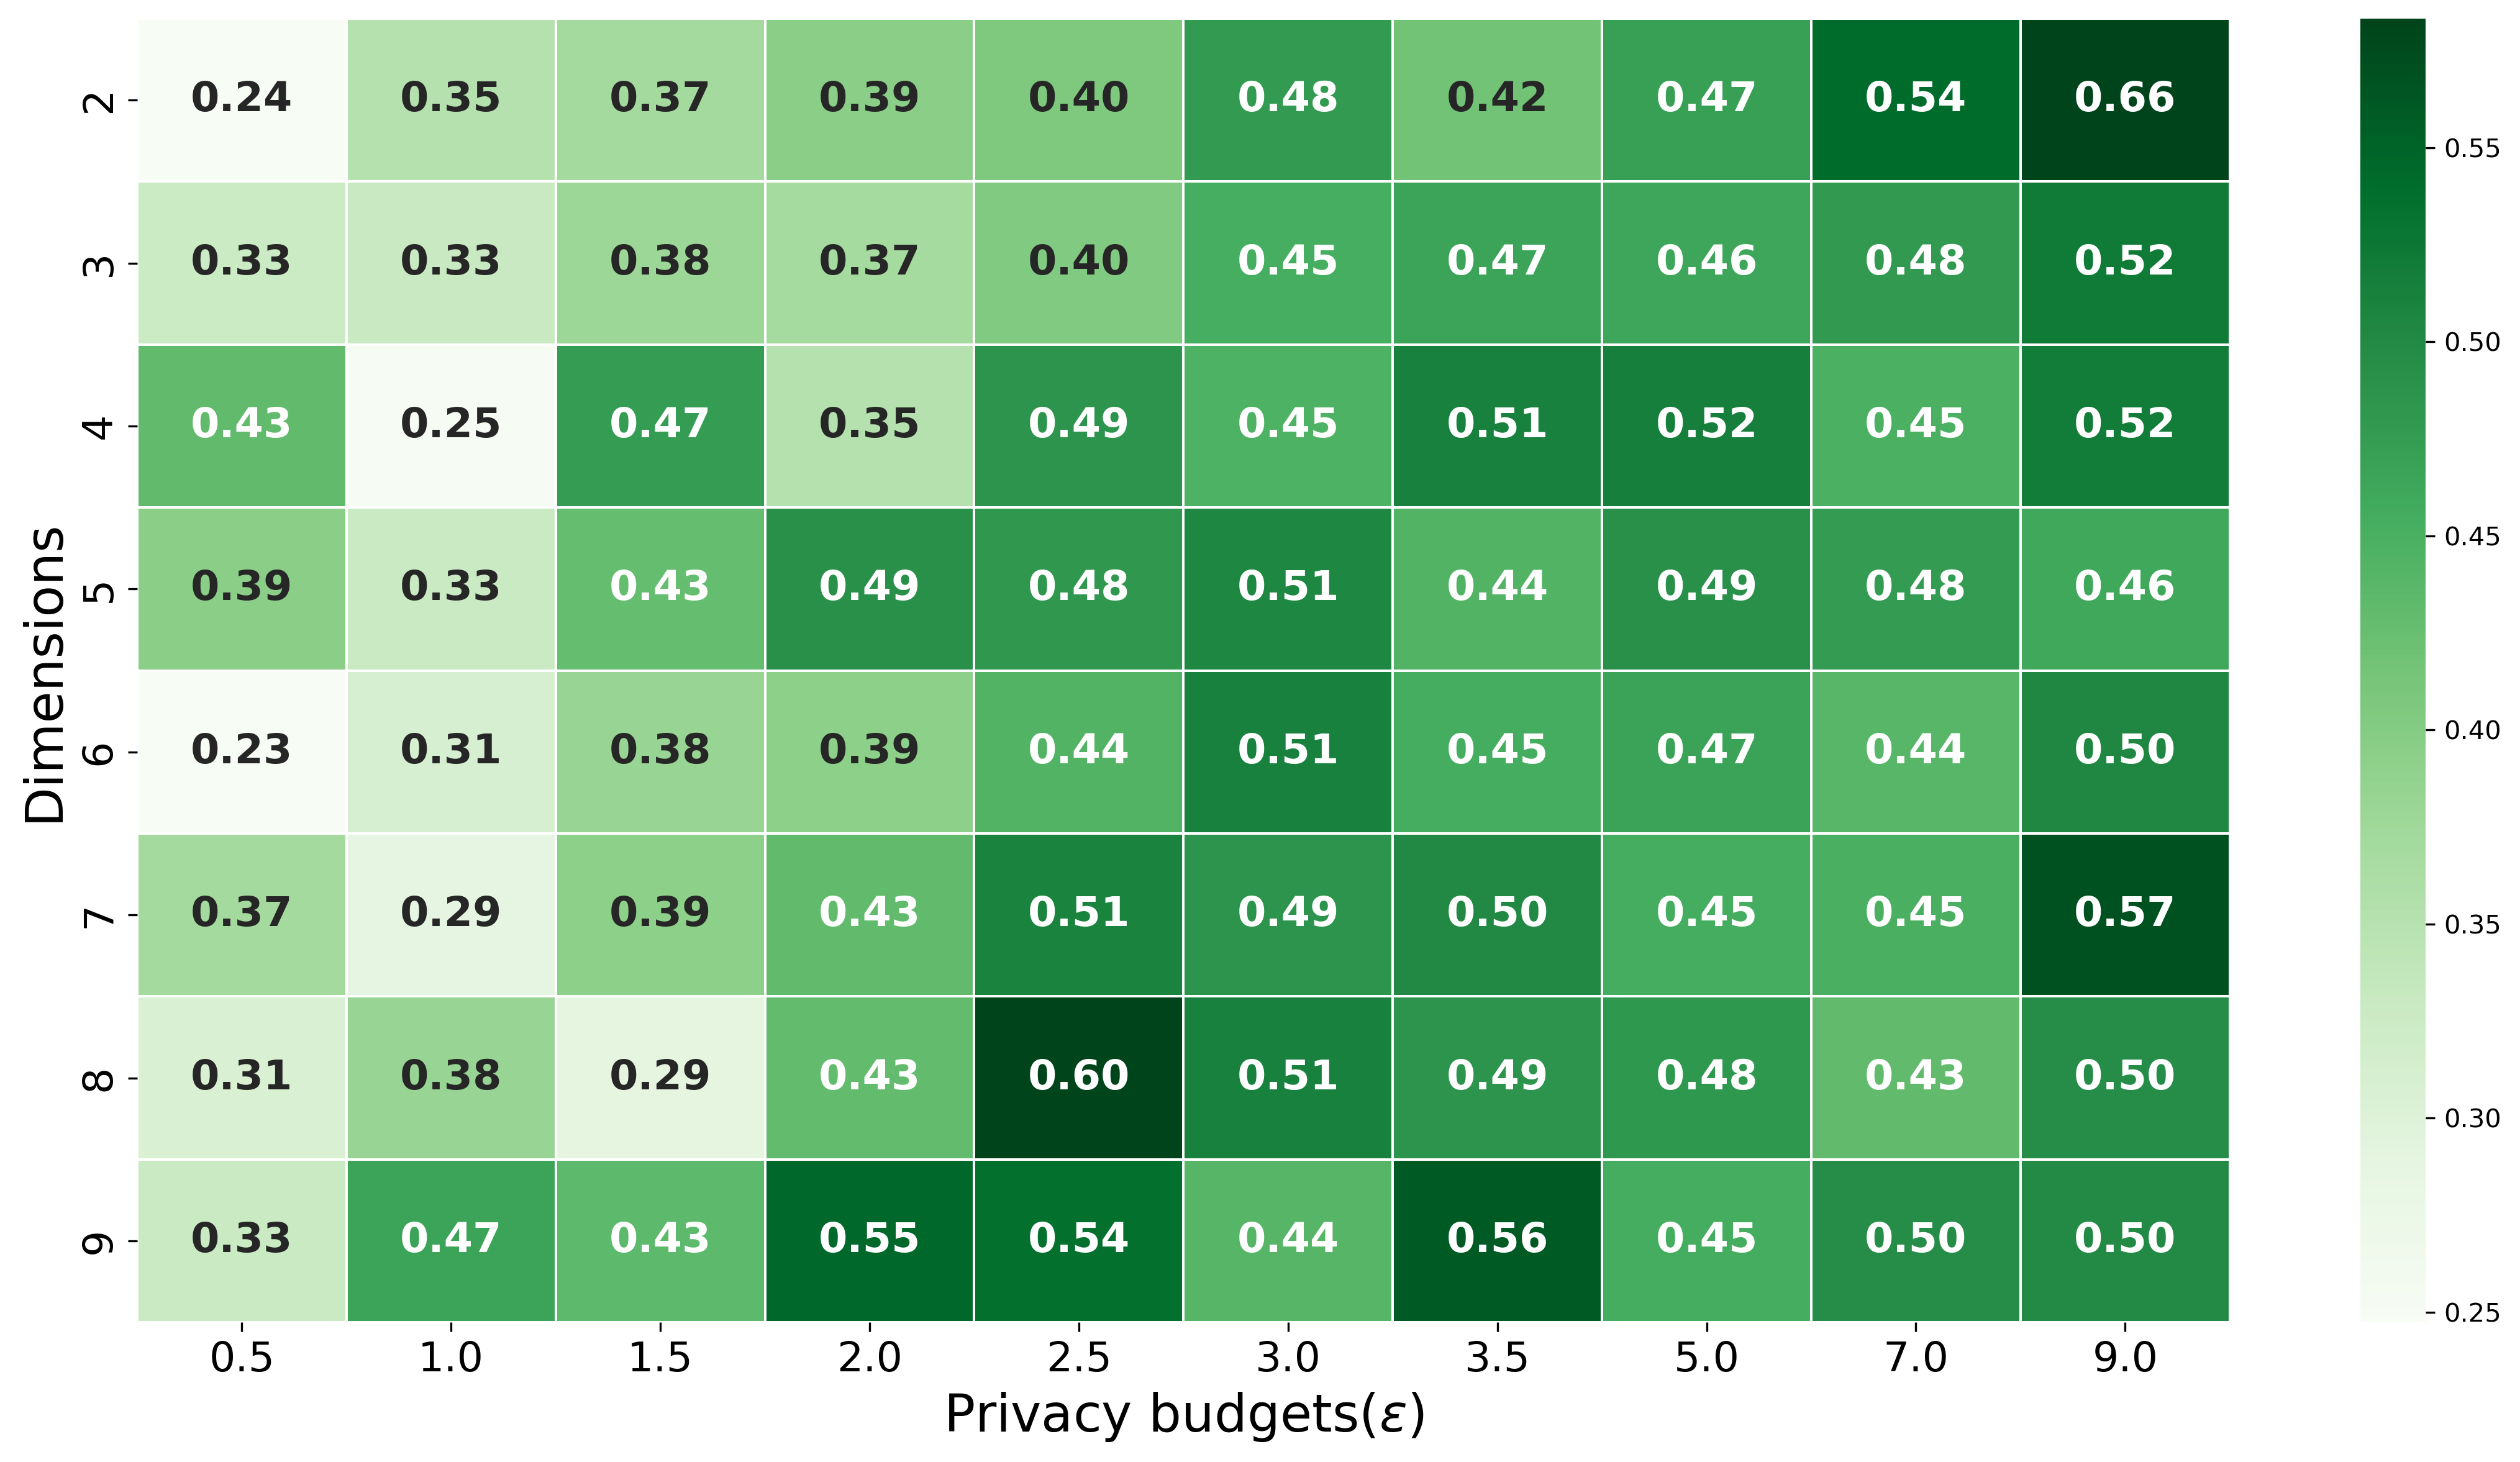
\includegraphics[width=1\textwidth]{Results/nd-laplace/piecewise/heart-dataset/tpr.png}
      \label{fig:privacy_tpr_heart-dataset_adversial_advantage_piecewise}
    \end{subfigure}
  \end{subfigure}
\end{figure}
For the Piecewise mechanism, the results are straightforward, mirroring the pattern observed with the membership advantage on the preceding page. While the bottom-left corner deviates slightly from the membership advantage, it's not strikingly irregular. As anticipated, the \gls{tpr} rises with an increasing privacy budget. Dimensionality does not significantly impact this, though the 2-dimensional data stands out with a notably higher value.
This happens for both mechanisms, so this is probably related to the choice in cluster features for 2-dimensional data.
%\todo[inline]{Investigate the impact of mi on 2-dimensional data}.

In contrast, the nD-Laplace mechanism presents a more diverse set of results. On the whole, there are not any drastic shifts, but there's a subtle trend of the membership advantage growing with a higher privacy budget. %Interestingly, the 3-dimensional data scores approximately 0.5 points lower than the others, warranting further investigation. \todo[inline]{Delve deeper into this discrepancy}.
Overall, Piecewise shows a higher privacy in comparison to nD-Laplace. This is in line with a higher utility that nD-Laplace offers.
\newpage

\subsection{Circle dataset}
\begin{figure}[H]
  \centering
  \begin{subfigure}[b]{0.85\textwidth}
    \begin{subfigure}[c]{1\textwidth}
      \caption{\textbf{Heatmap showing adversary advantage for the nD-Laplace mechanism, per privacy budget \& dimension for circle-dataset.}}
      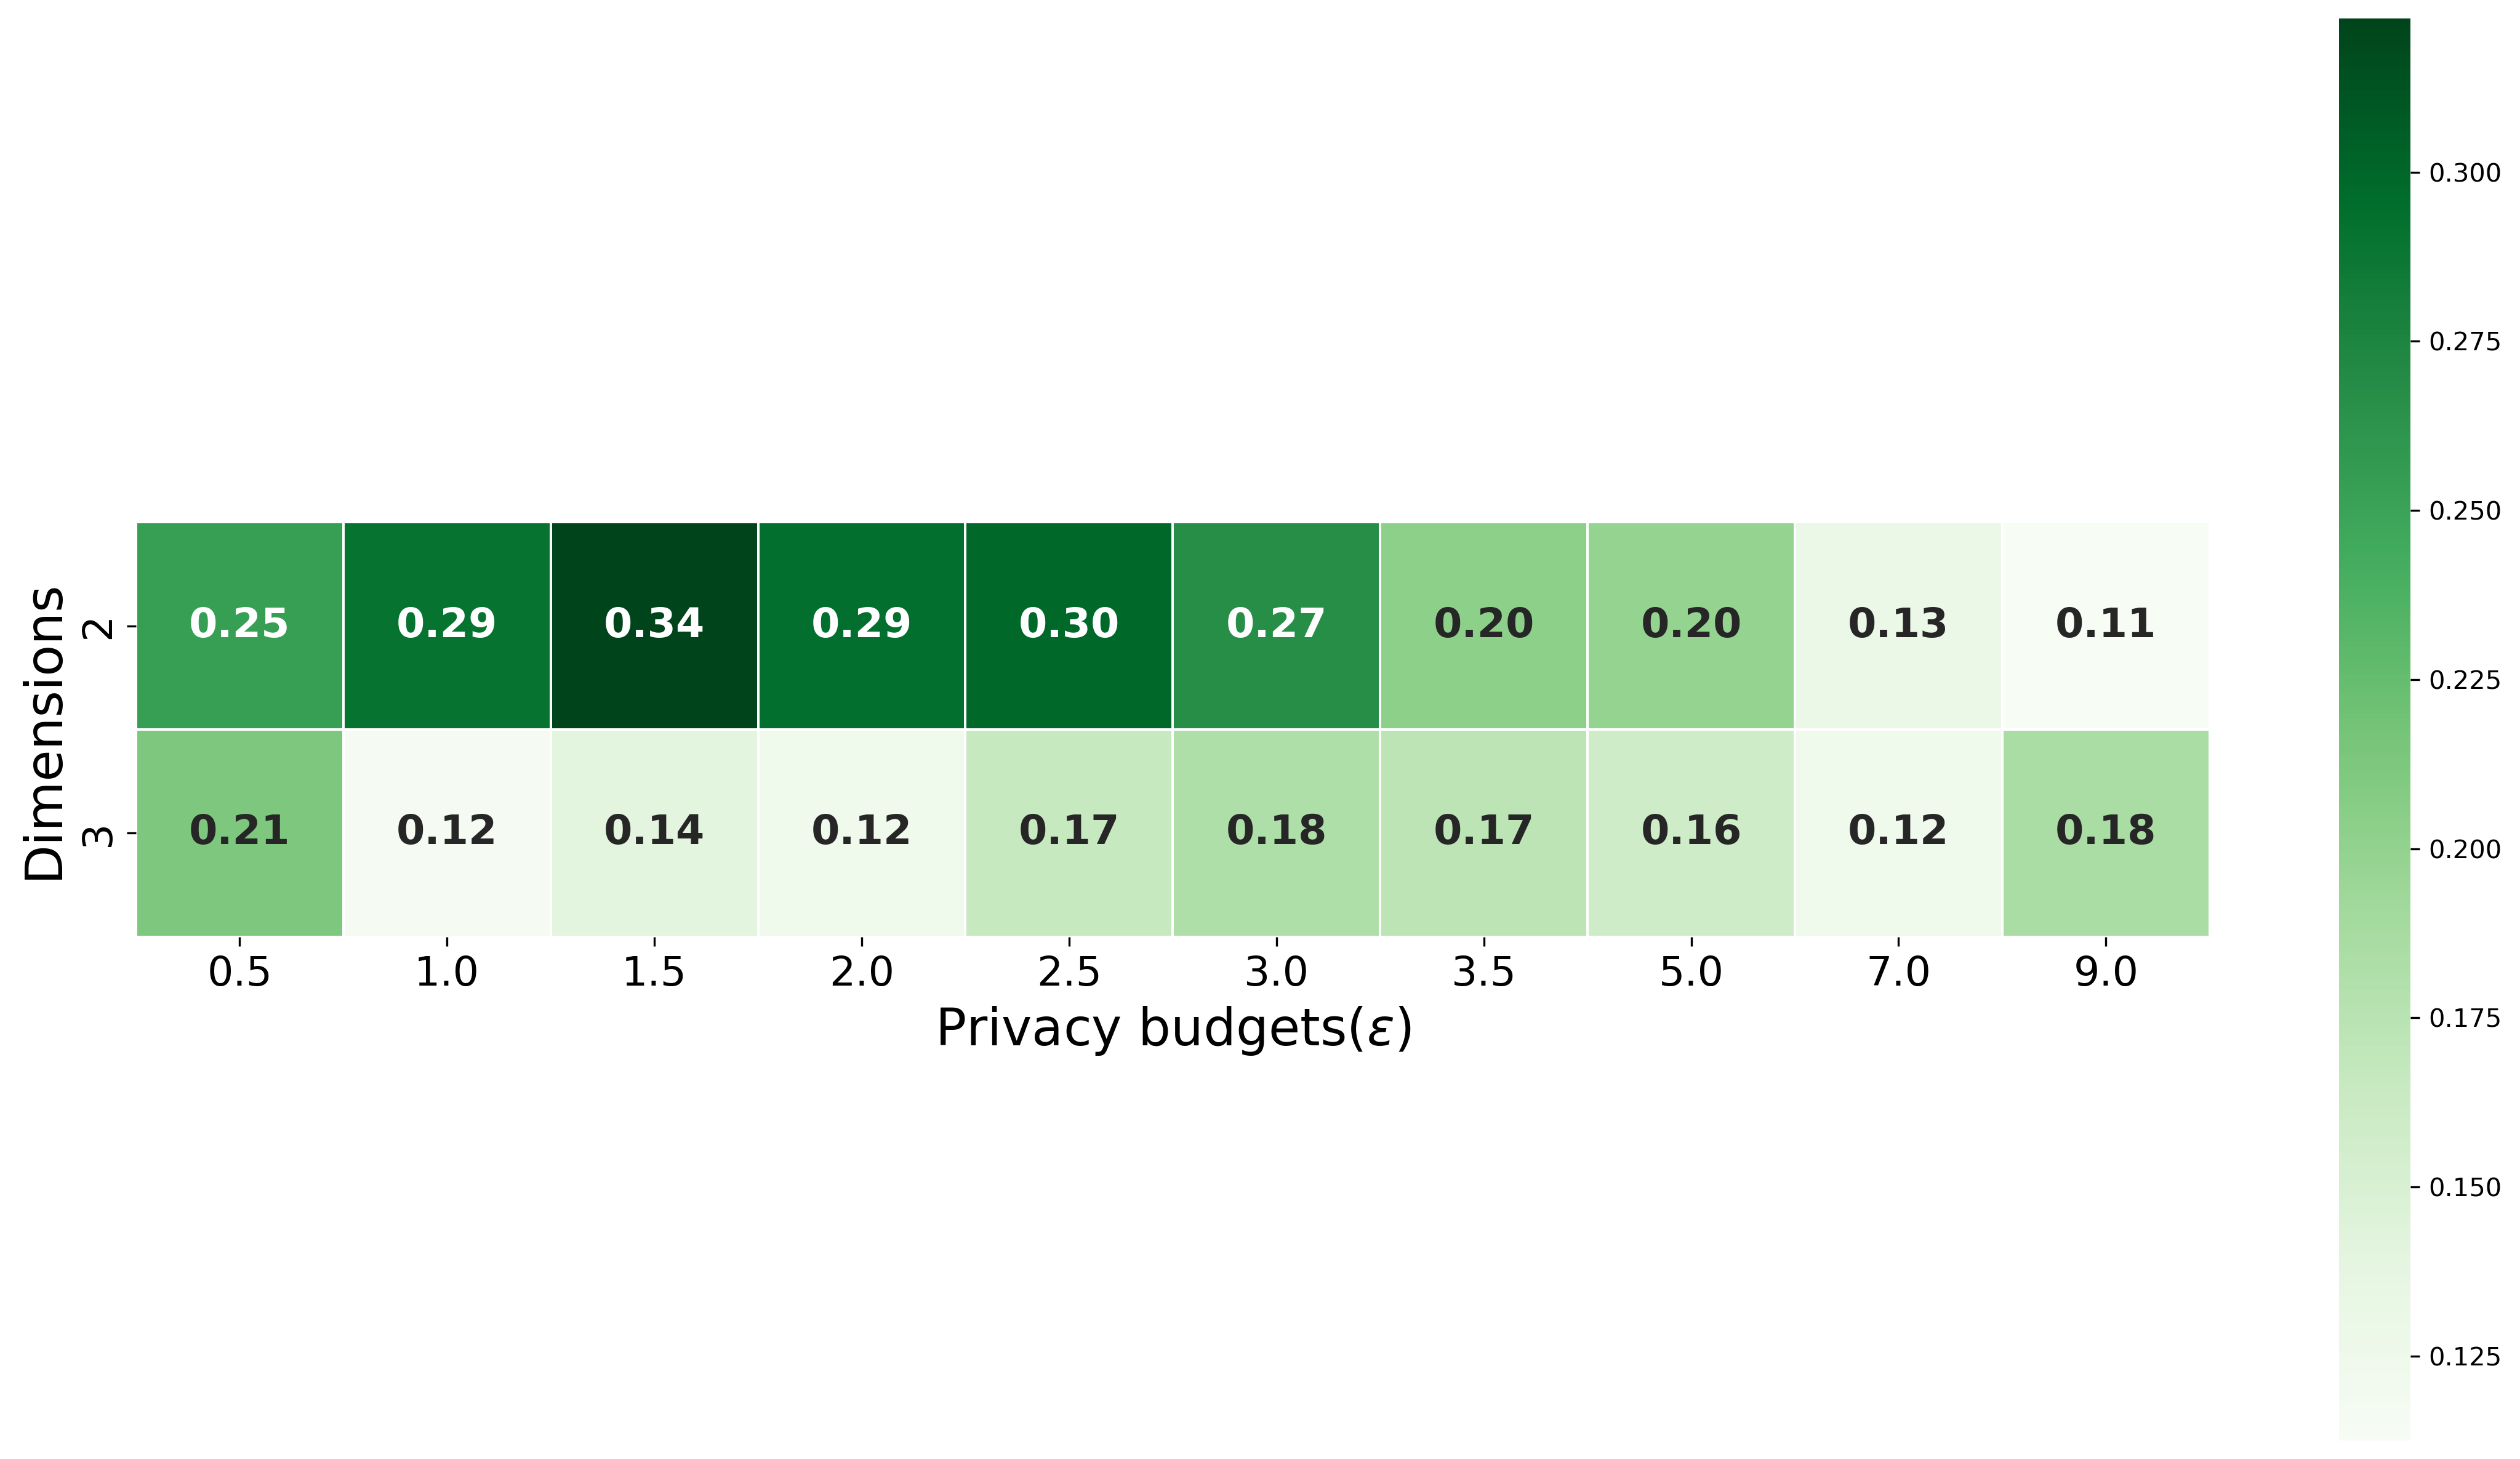
\includegraphics[width=1\textwidth]{Results/nd-laplace/nd-Laplace/circle-dataset/attack_adv.png}
      \label{fig:privacy_circle-dataset_adversial_advantage_kd-laplace}
    \end{subfigure}
    \vfill % vertical space
    \begin{subfigure}[c]{1\textwidth}
      \caption{\textbf{Heatmap showing adversary advantage for the Piecewise mechanism, per privacy budget \& dimension for seeds-dataset.}}
      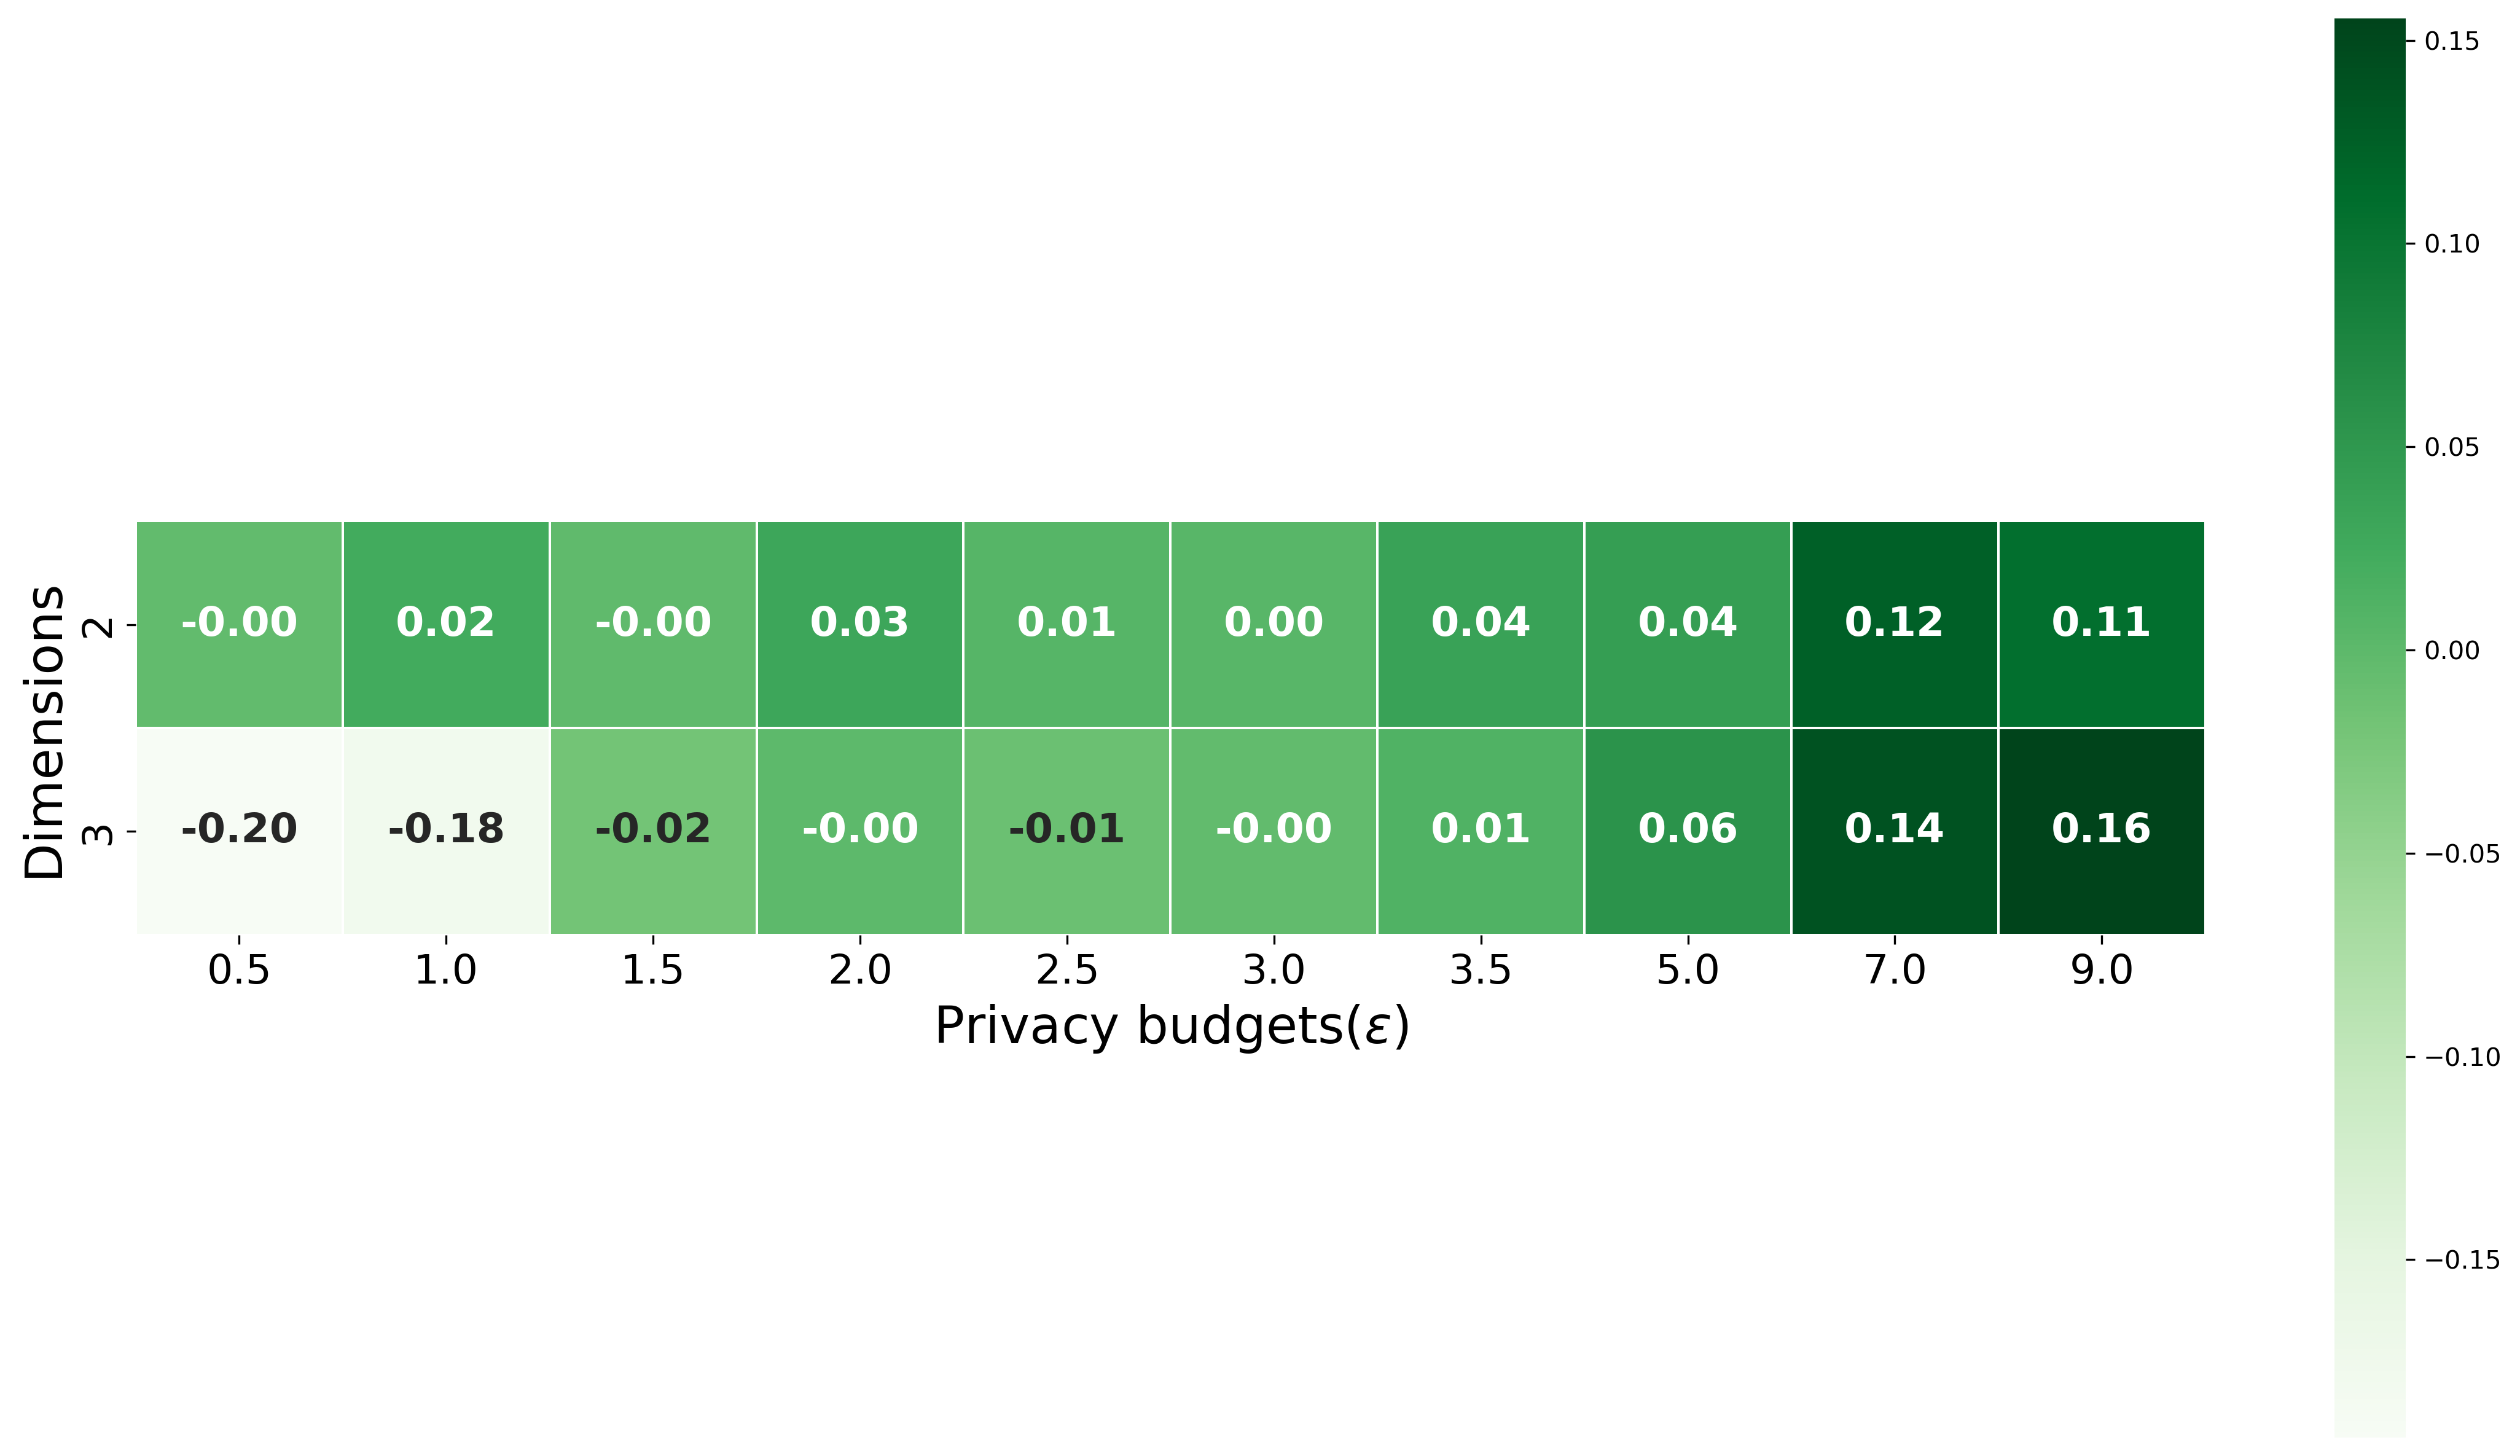
\includegraphics[width=1\textwidth]{Results/nd-laplace/piecewise/circle-dataset/attack_adv.png}
      \label{fig:privacy_circle-dataset_adversial_advantage_piecewise}
    \end{subfigure}
  \end{subfigure}
\end{figure}
For the nD-Laplace method, it's hard to see a clear trend. There's a small increase with a higher privacy budget, but it's only by 0.1 to 0.2. These numbers match the \gls{ami} scores, which are around 0.3 to 0.4. So, if the data has low utility, there's not much information that can be leaked.

For the Piecewise method, things are a bit clearer. When the privacy budget goes up, the advantage also goes up. But there's something odd for epsilon values of 0.5 and 1 with 3-dimensional data. We will look into this more by checking the \gls{tpr} on the next page.

\newpage
\begin{figure}[H]
  \centering
  \begin{subfigure}[b]{0.9\textwidth}
    \begin{subfigure}[c]{1\textwidth}
      \caption{\textbf{Heatmap TPR for the nD-Laplace mechanism, per privacy budget \& dimension for Circle-dataset.}}
      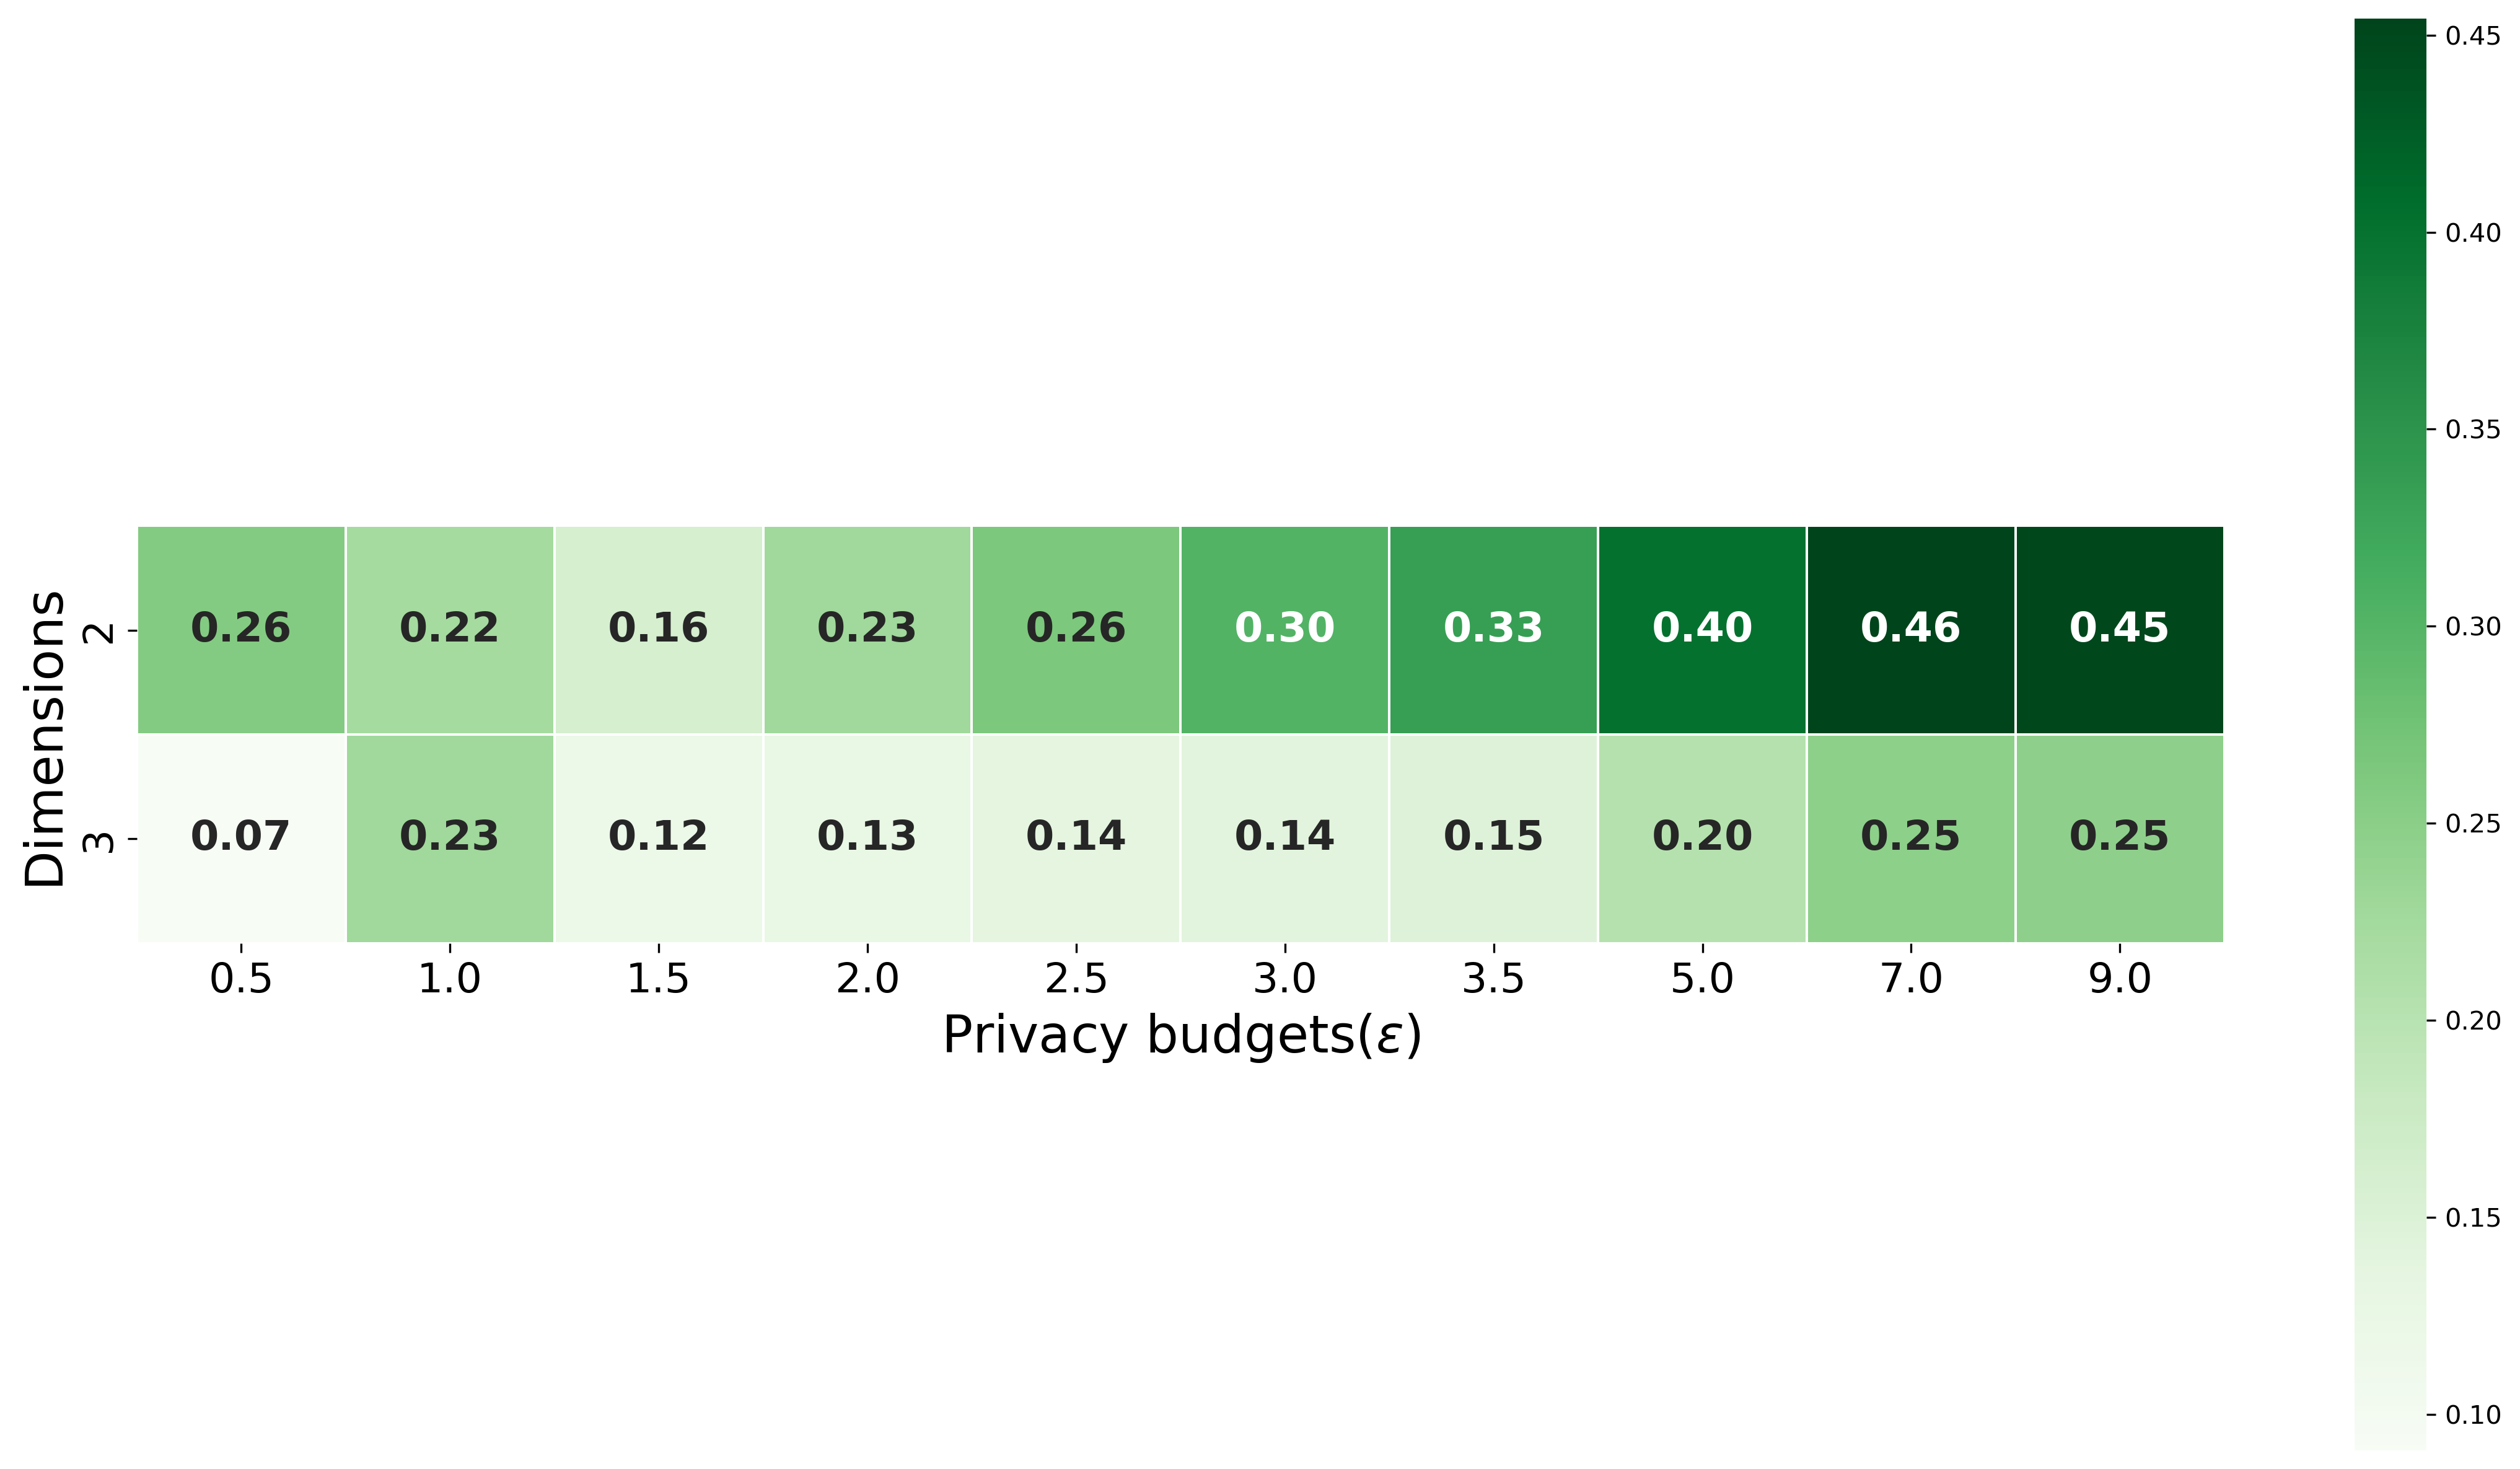
\includegraphics[width=1\textwidth]{Results/nd-laplace/nd-Laplace/circle-dataset/tpr.png}
      \label{fig:privacy_tpr_circle-dataset_adversial_advantage_kd-laplace}
    \end{subfigure}
    \vfill % vertical space

    \begin{subfigure}[c]{1\textwidth}
      \caption{\textbf{Heatmap TPR for the Piecewise mechanism, per privacy budget \& dimension for Circle-dataset.}}
      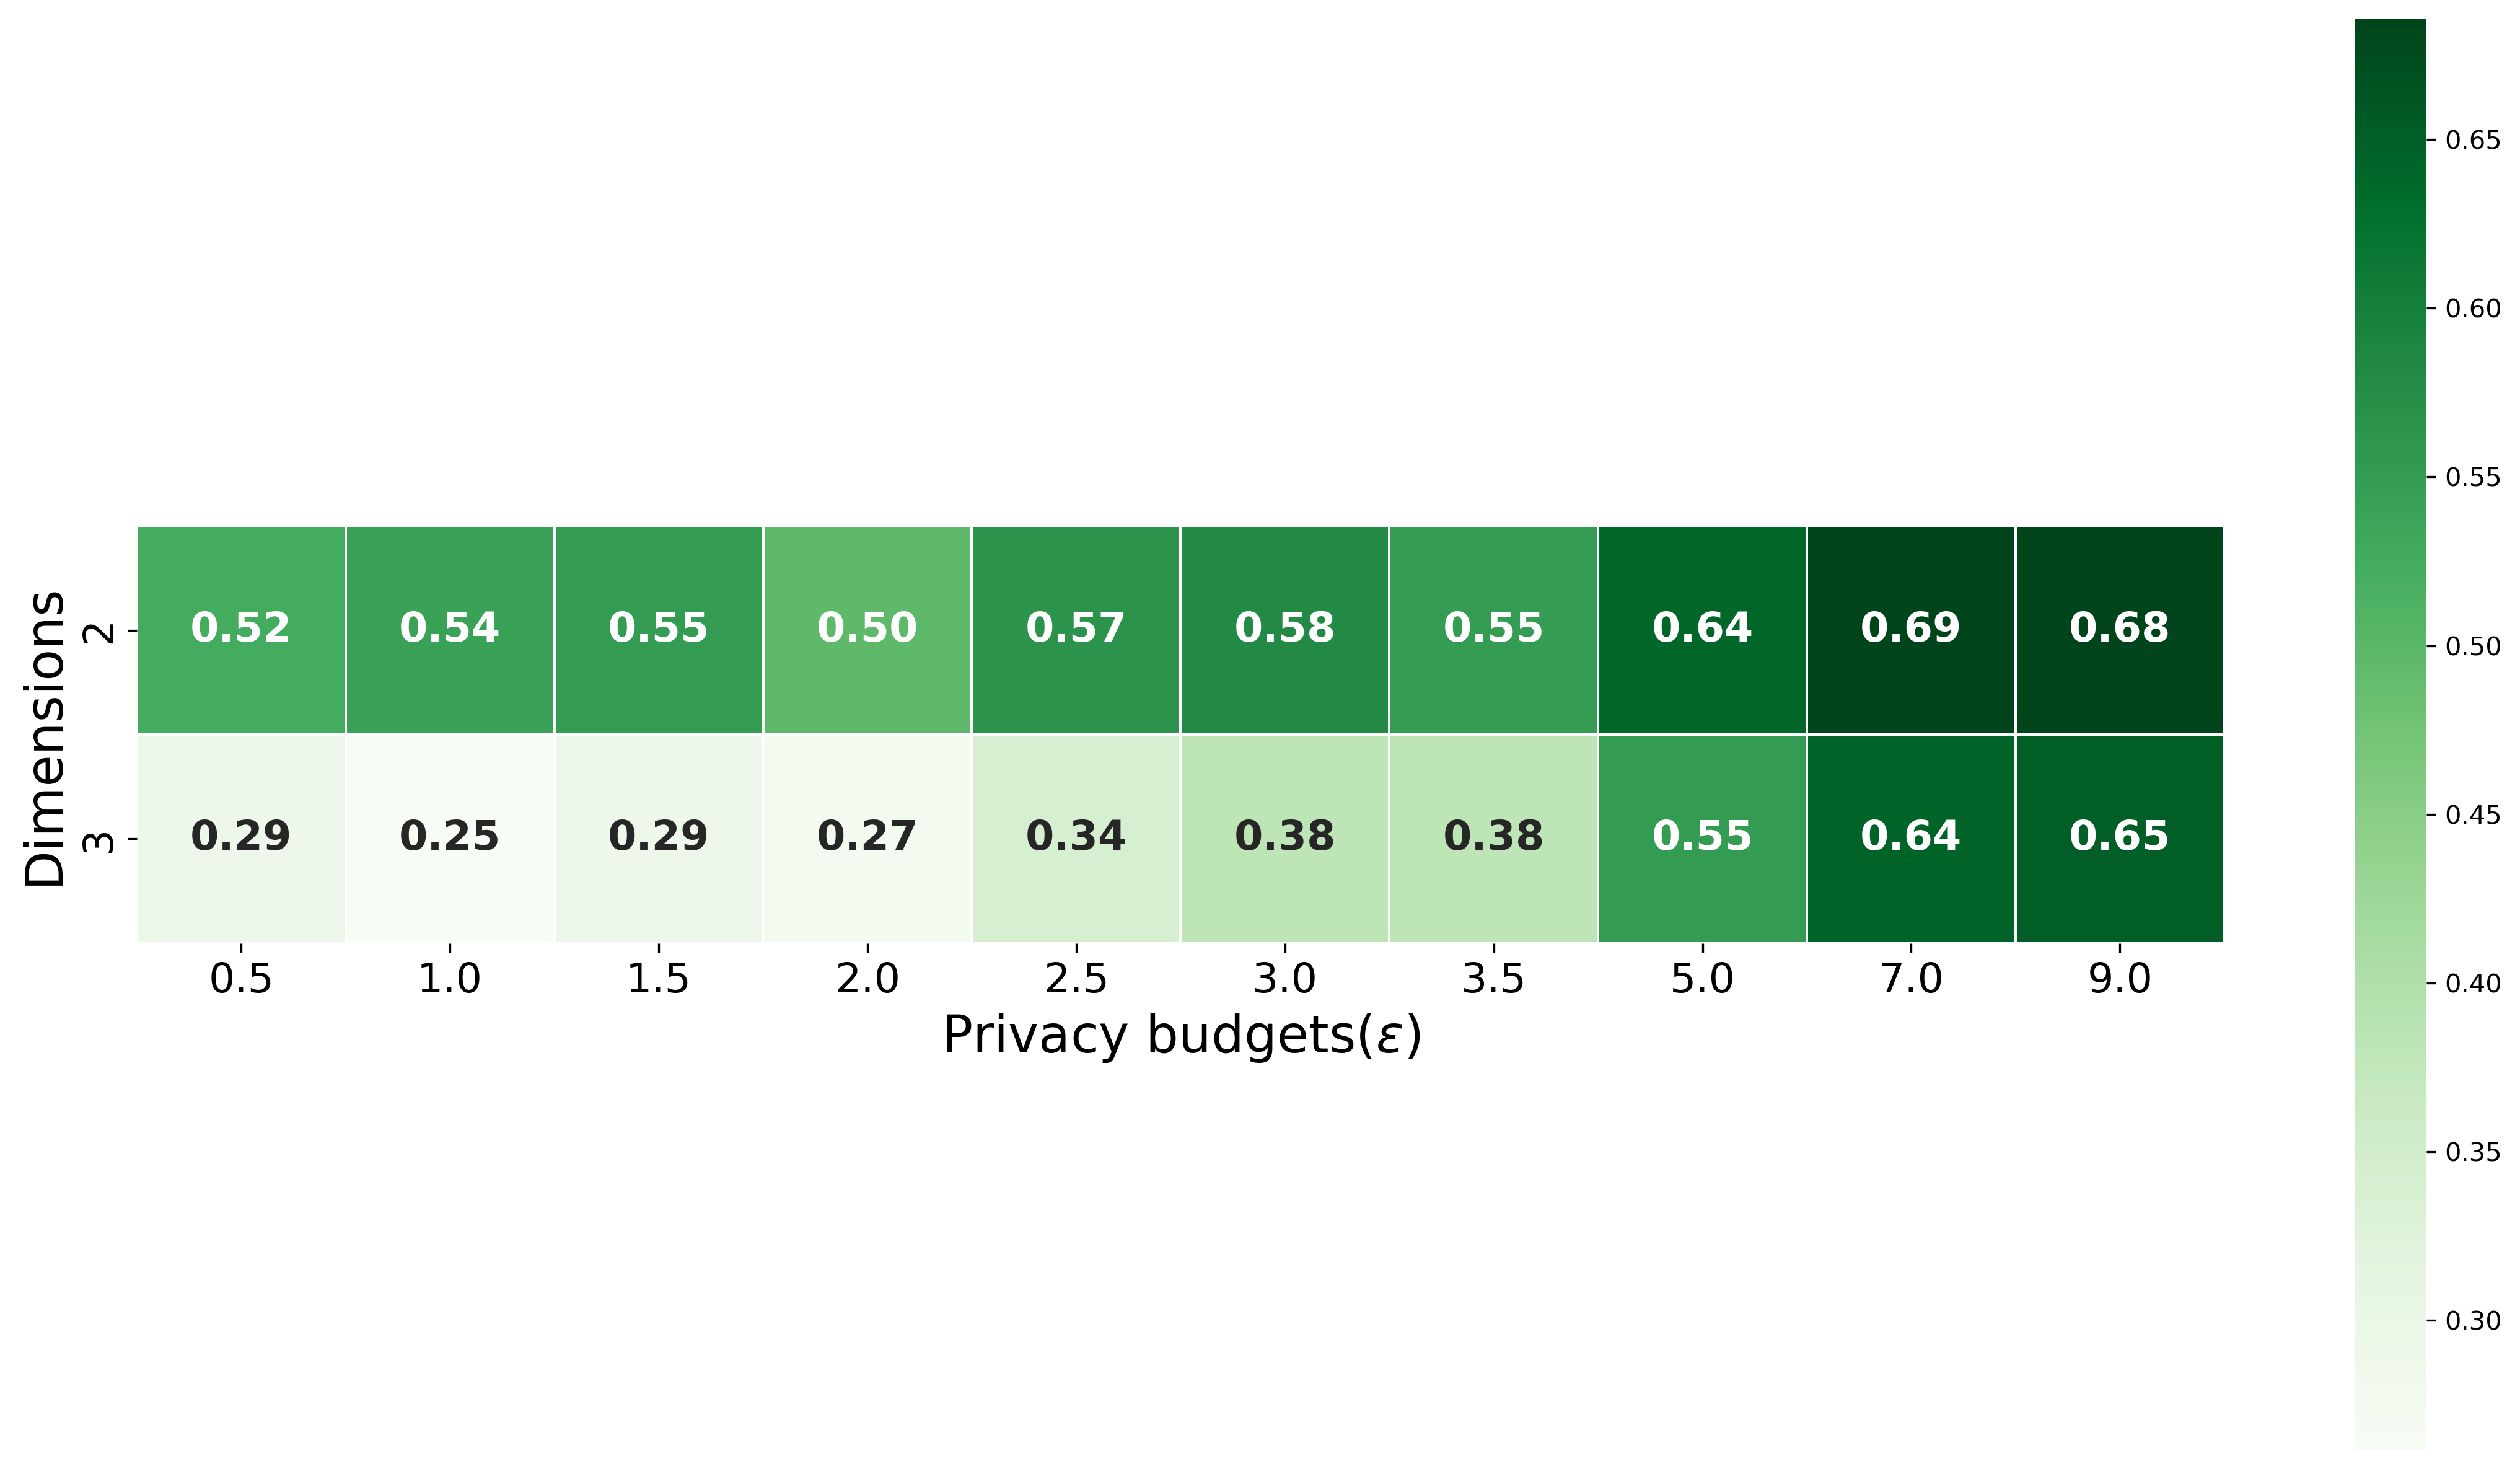
\includegraphics[width=1\textwidth]{Results/nd-laplace/piecewise/circle-dataset/tpr.png}
      \label{fig:privacy_tpr_circle-dataset_adversial_advantage_piecewise}
    \end{subfigure}
  \end{subfigure}
\end{figure}
In our examination of the nD-Laplace mechanism, it's clear that both the privacy budgets and the dimensions have a notable impact on the \gls{tpr}. Specifically, two-dimensional data tends to reveal more information than three-dimensional data. On the other hand, the Piecewise mechanism shows a similar trend, but its \gls{tpr} is generally about 0.10 higher. An exception is seen for the lower epsilon values of 0.5 - 1, where the nD-Laplace mechanism has a greater membership advantage.

We also noticed an inconsistency for the Piecewise mechanism with three-dimensional data at privacy budgets of 0.5 and 1. However, the \gls{tpr} for these values seems to be consistent. This suggests that the \gls{fpr} might be higher for these settings. As a result, the membership advantage (defined as $tpr - fpr$) is below zero, even though the \gls{tpr} is higher.
\newpage
\subsection{Line dataset}
\begin{figure}[H]
  \centering
  \begin{subfigure}[b]{0.80\textwidth}
    \begin{subfigure}[c]{1\textwidth}
      \caption{\textbf{Heatmap showing adversary advantage for the nD-Laplace mechanism, per privacy budget \& dimension for seeds-dataset.}}
      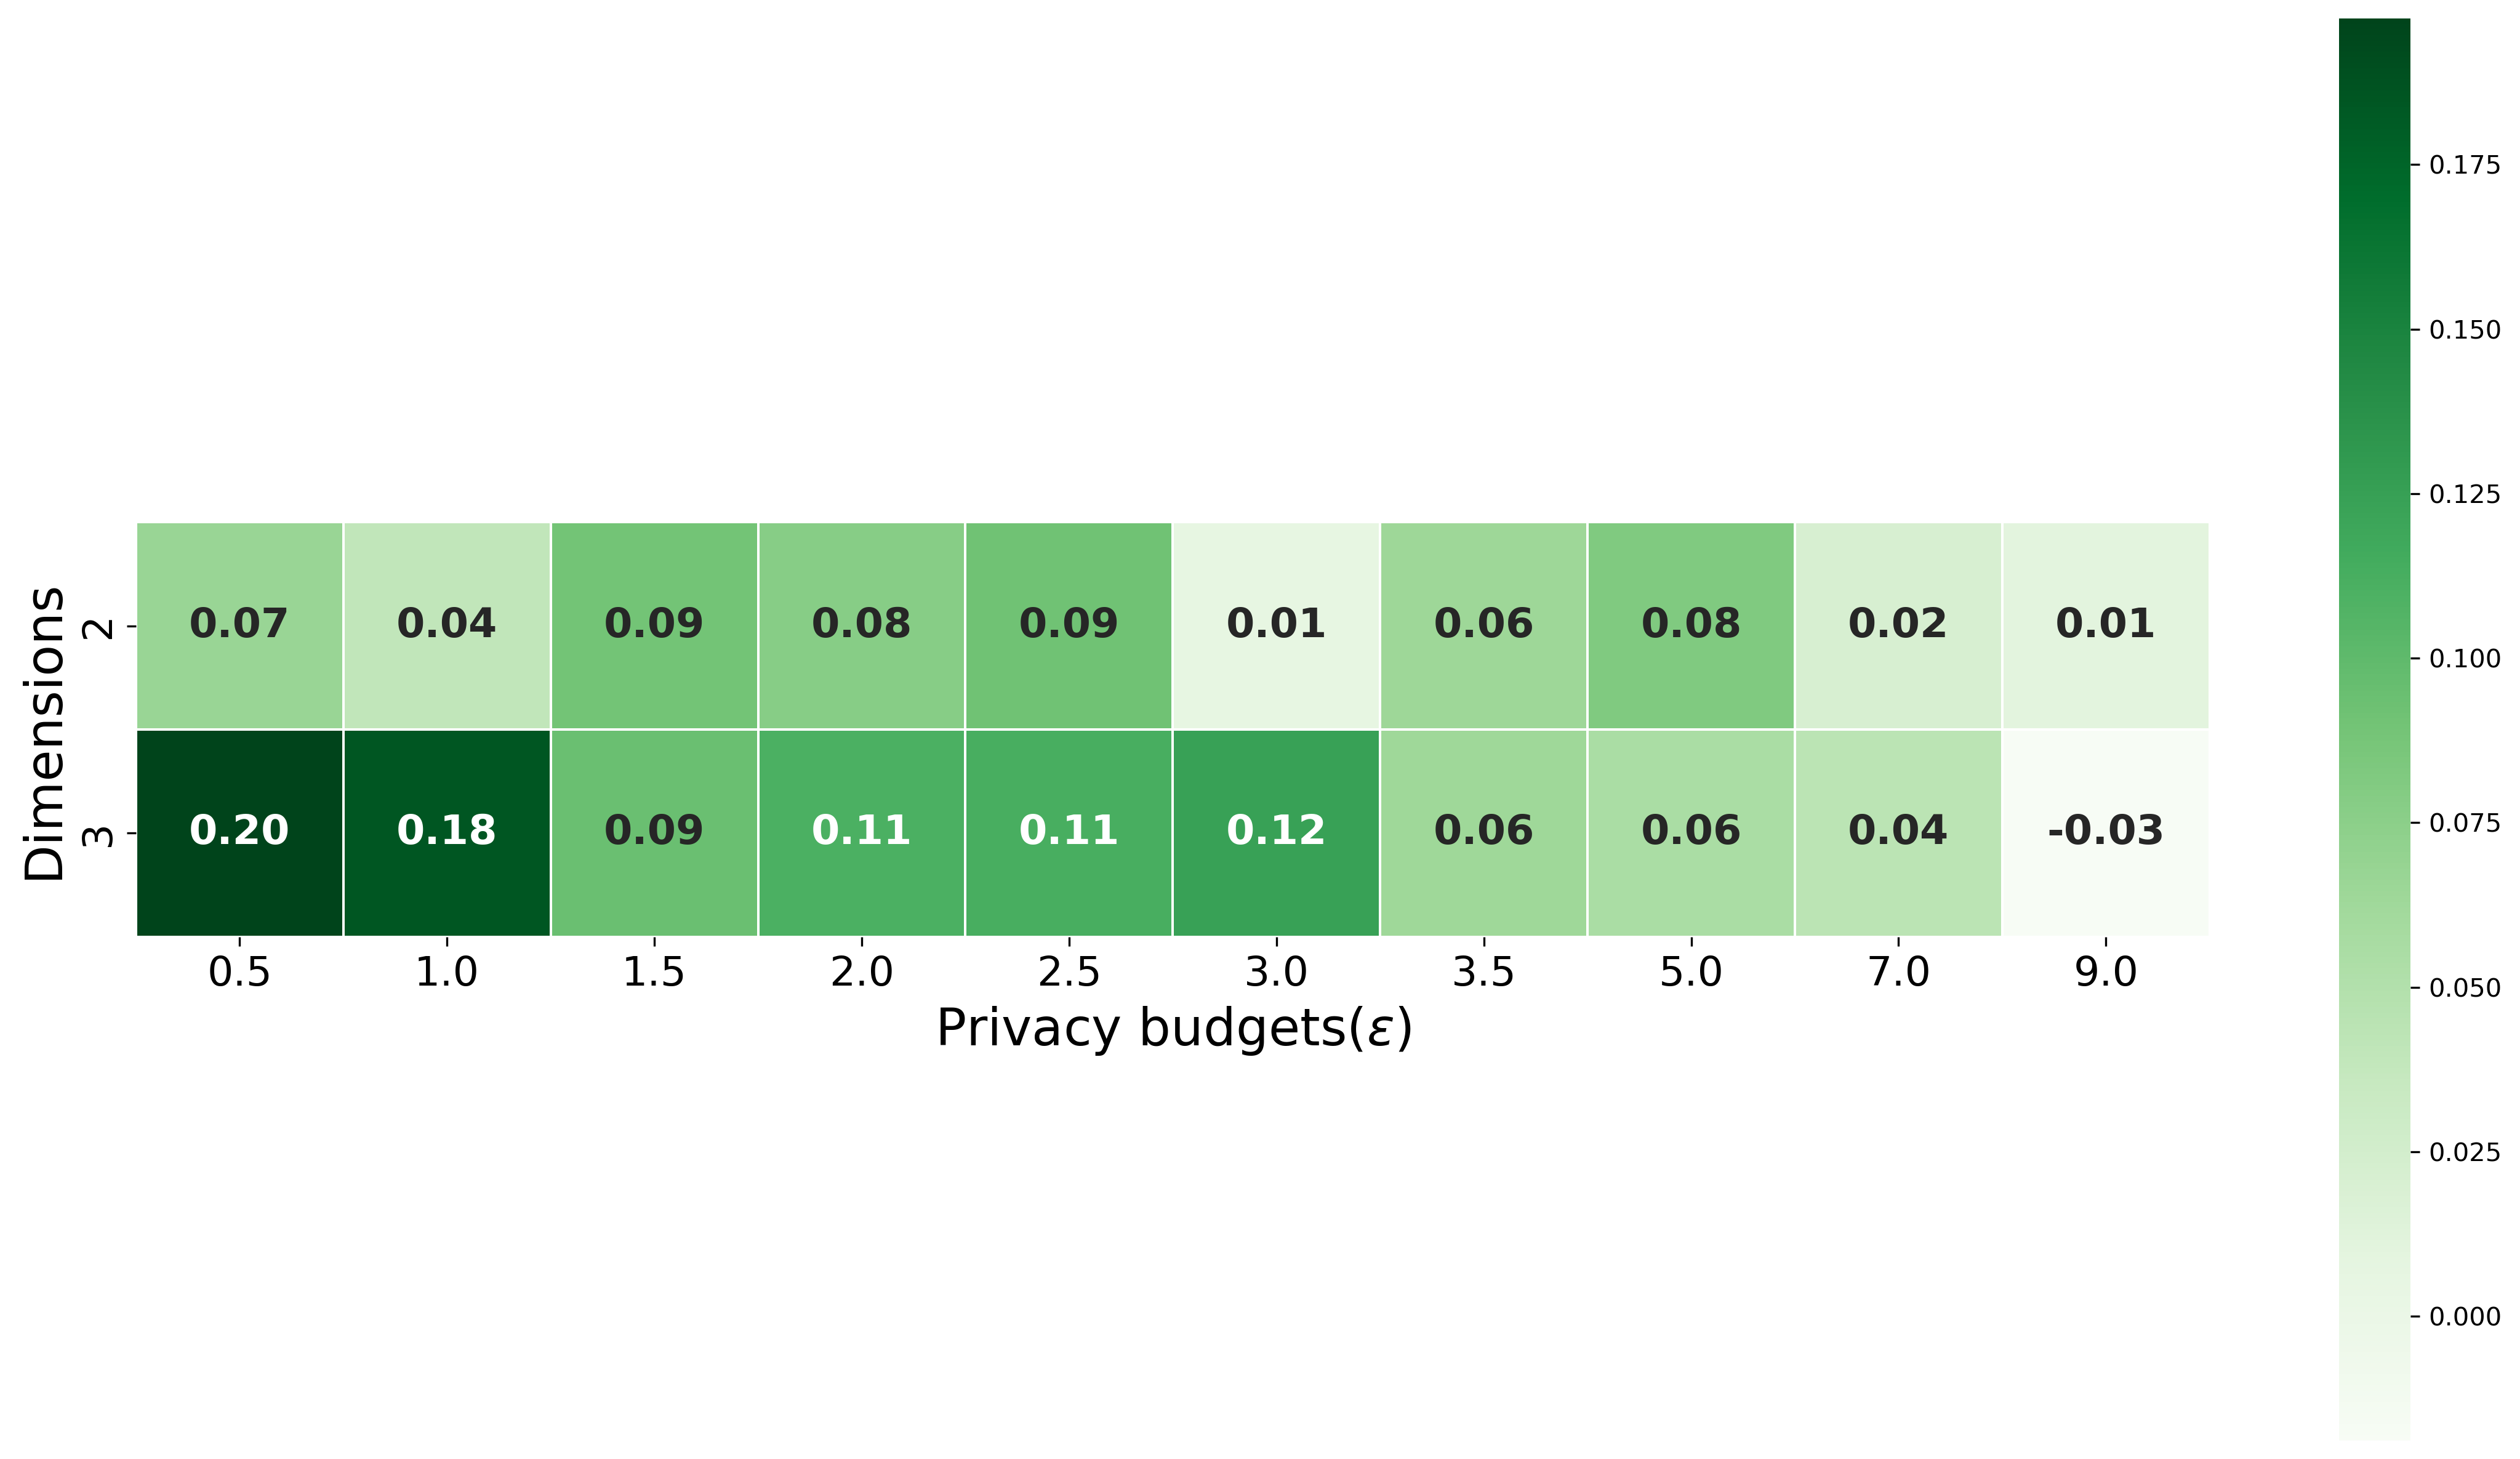
\includegraphics[width=1\textwidth]{Results/nd-laplace/nd-Laplace/line-dataset/attack_adv.png}
      \label{fig:privacy_line-dataset_adversial_advantage_kd-laplace}
    \end{subfigure}
    \vfill % vertical space

    \begin{subfigure}[c]{1\textwidth}
      \caption{\textbf{Heatmap showing membership advantage for the Piecewise mechanism, per privacy budget \& dimension for seeds-dataset.}}
      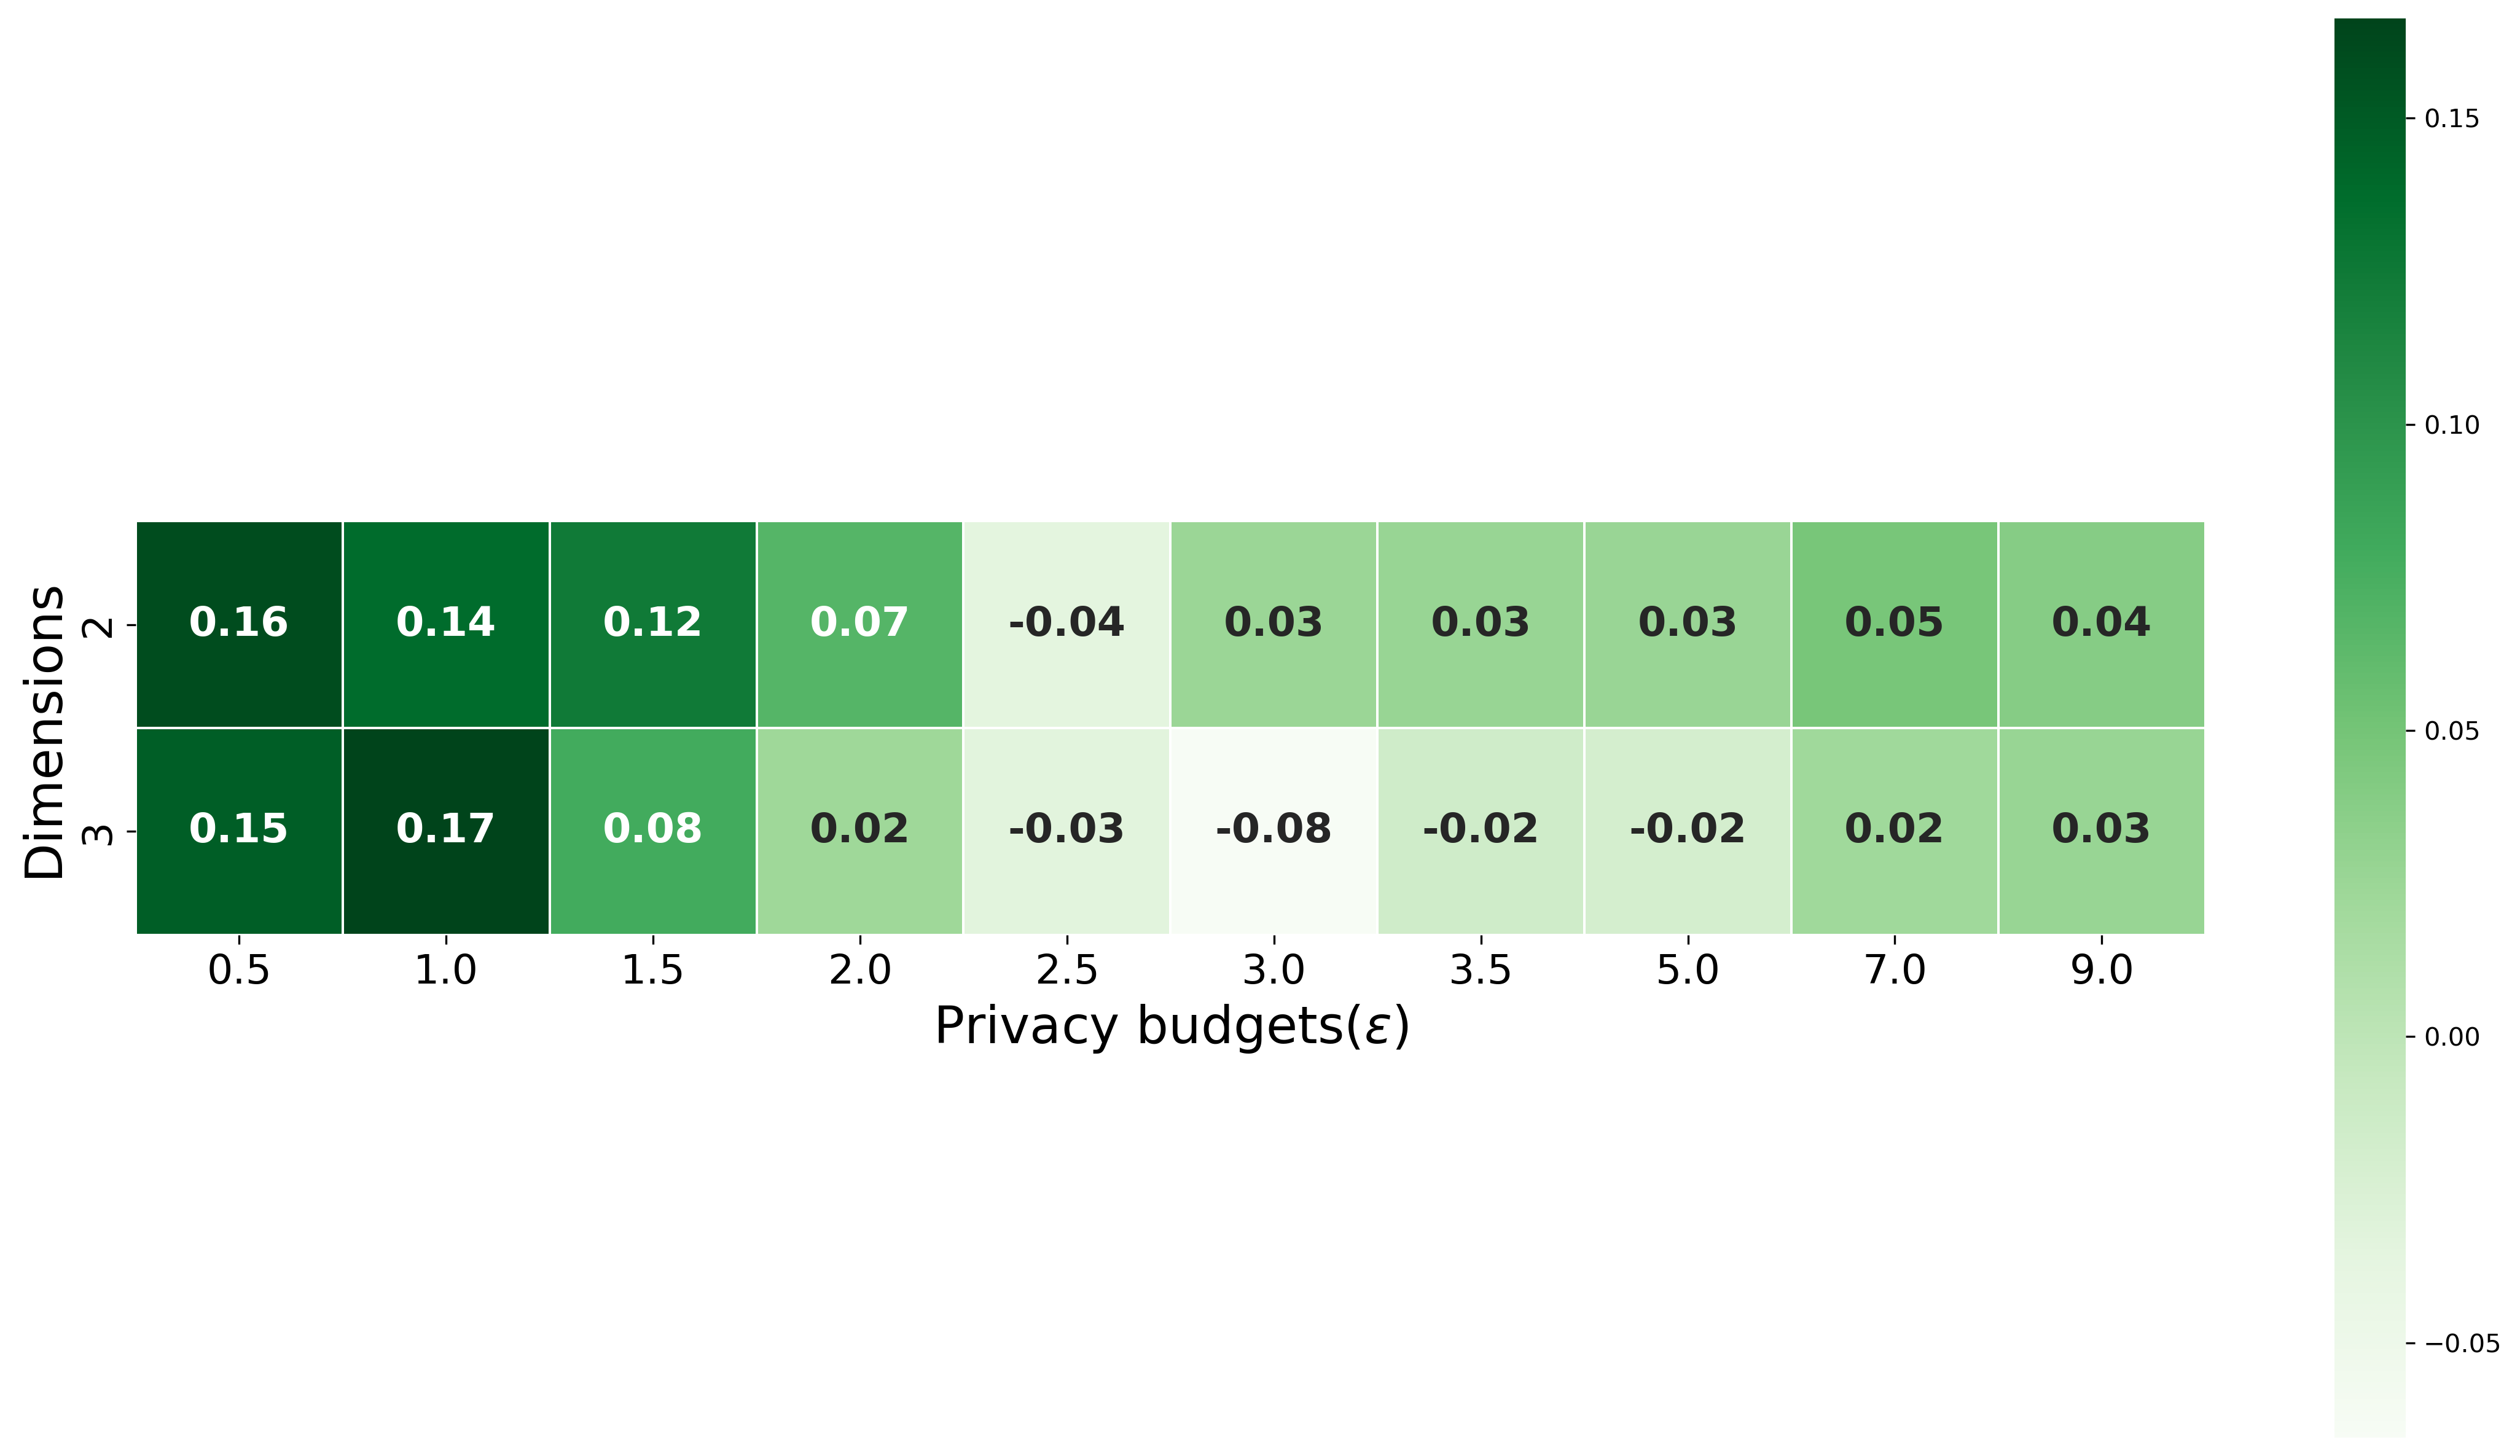
\includegraphics[width=1\textwidth]{Results/nd-laplace/piecewise/line-dataset/attack_adv.png}
      \label{fig:privacy_line-dataset_adversial_advantage_piecewise}
    \end{subfigure}
  \end{subfigure}
\end{figure}
The scores from both mechanisms largely align and neither exhibits a distinct pattern. However, for the nD-Laplace mechanism, two values stand out for the three-dimensional data: -0.09 and -0.10. These values are notably lower than the two-dimensional values for the same privacy budgets. Similarly, for the Piecewise mechanism, we observe this trend for both dimensions, but only for a privacy budget of 0.5.

To determine whether the \gls{tpr} displays consistent values, we will analyze this metric on the subsequent page.
\newpage
\begin{figure}[H]
  \centering
  \begin{subfigure}[b]{0.9\textwidth}
    \begin{subfigure}[c]{1\textwidth}
      \caption{\textbf{Heatmap TPR for the nD-Laplace mechanism, per privacy budget \& dimension for line-dataset.}}
      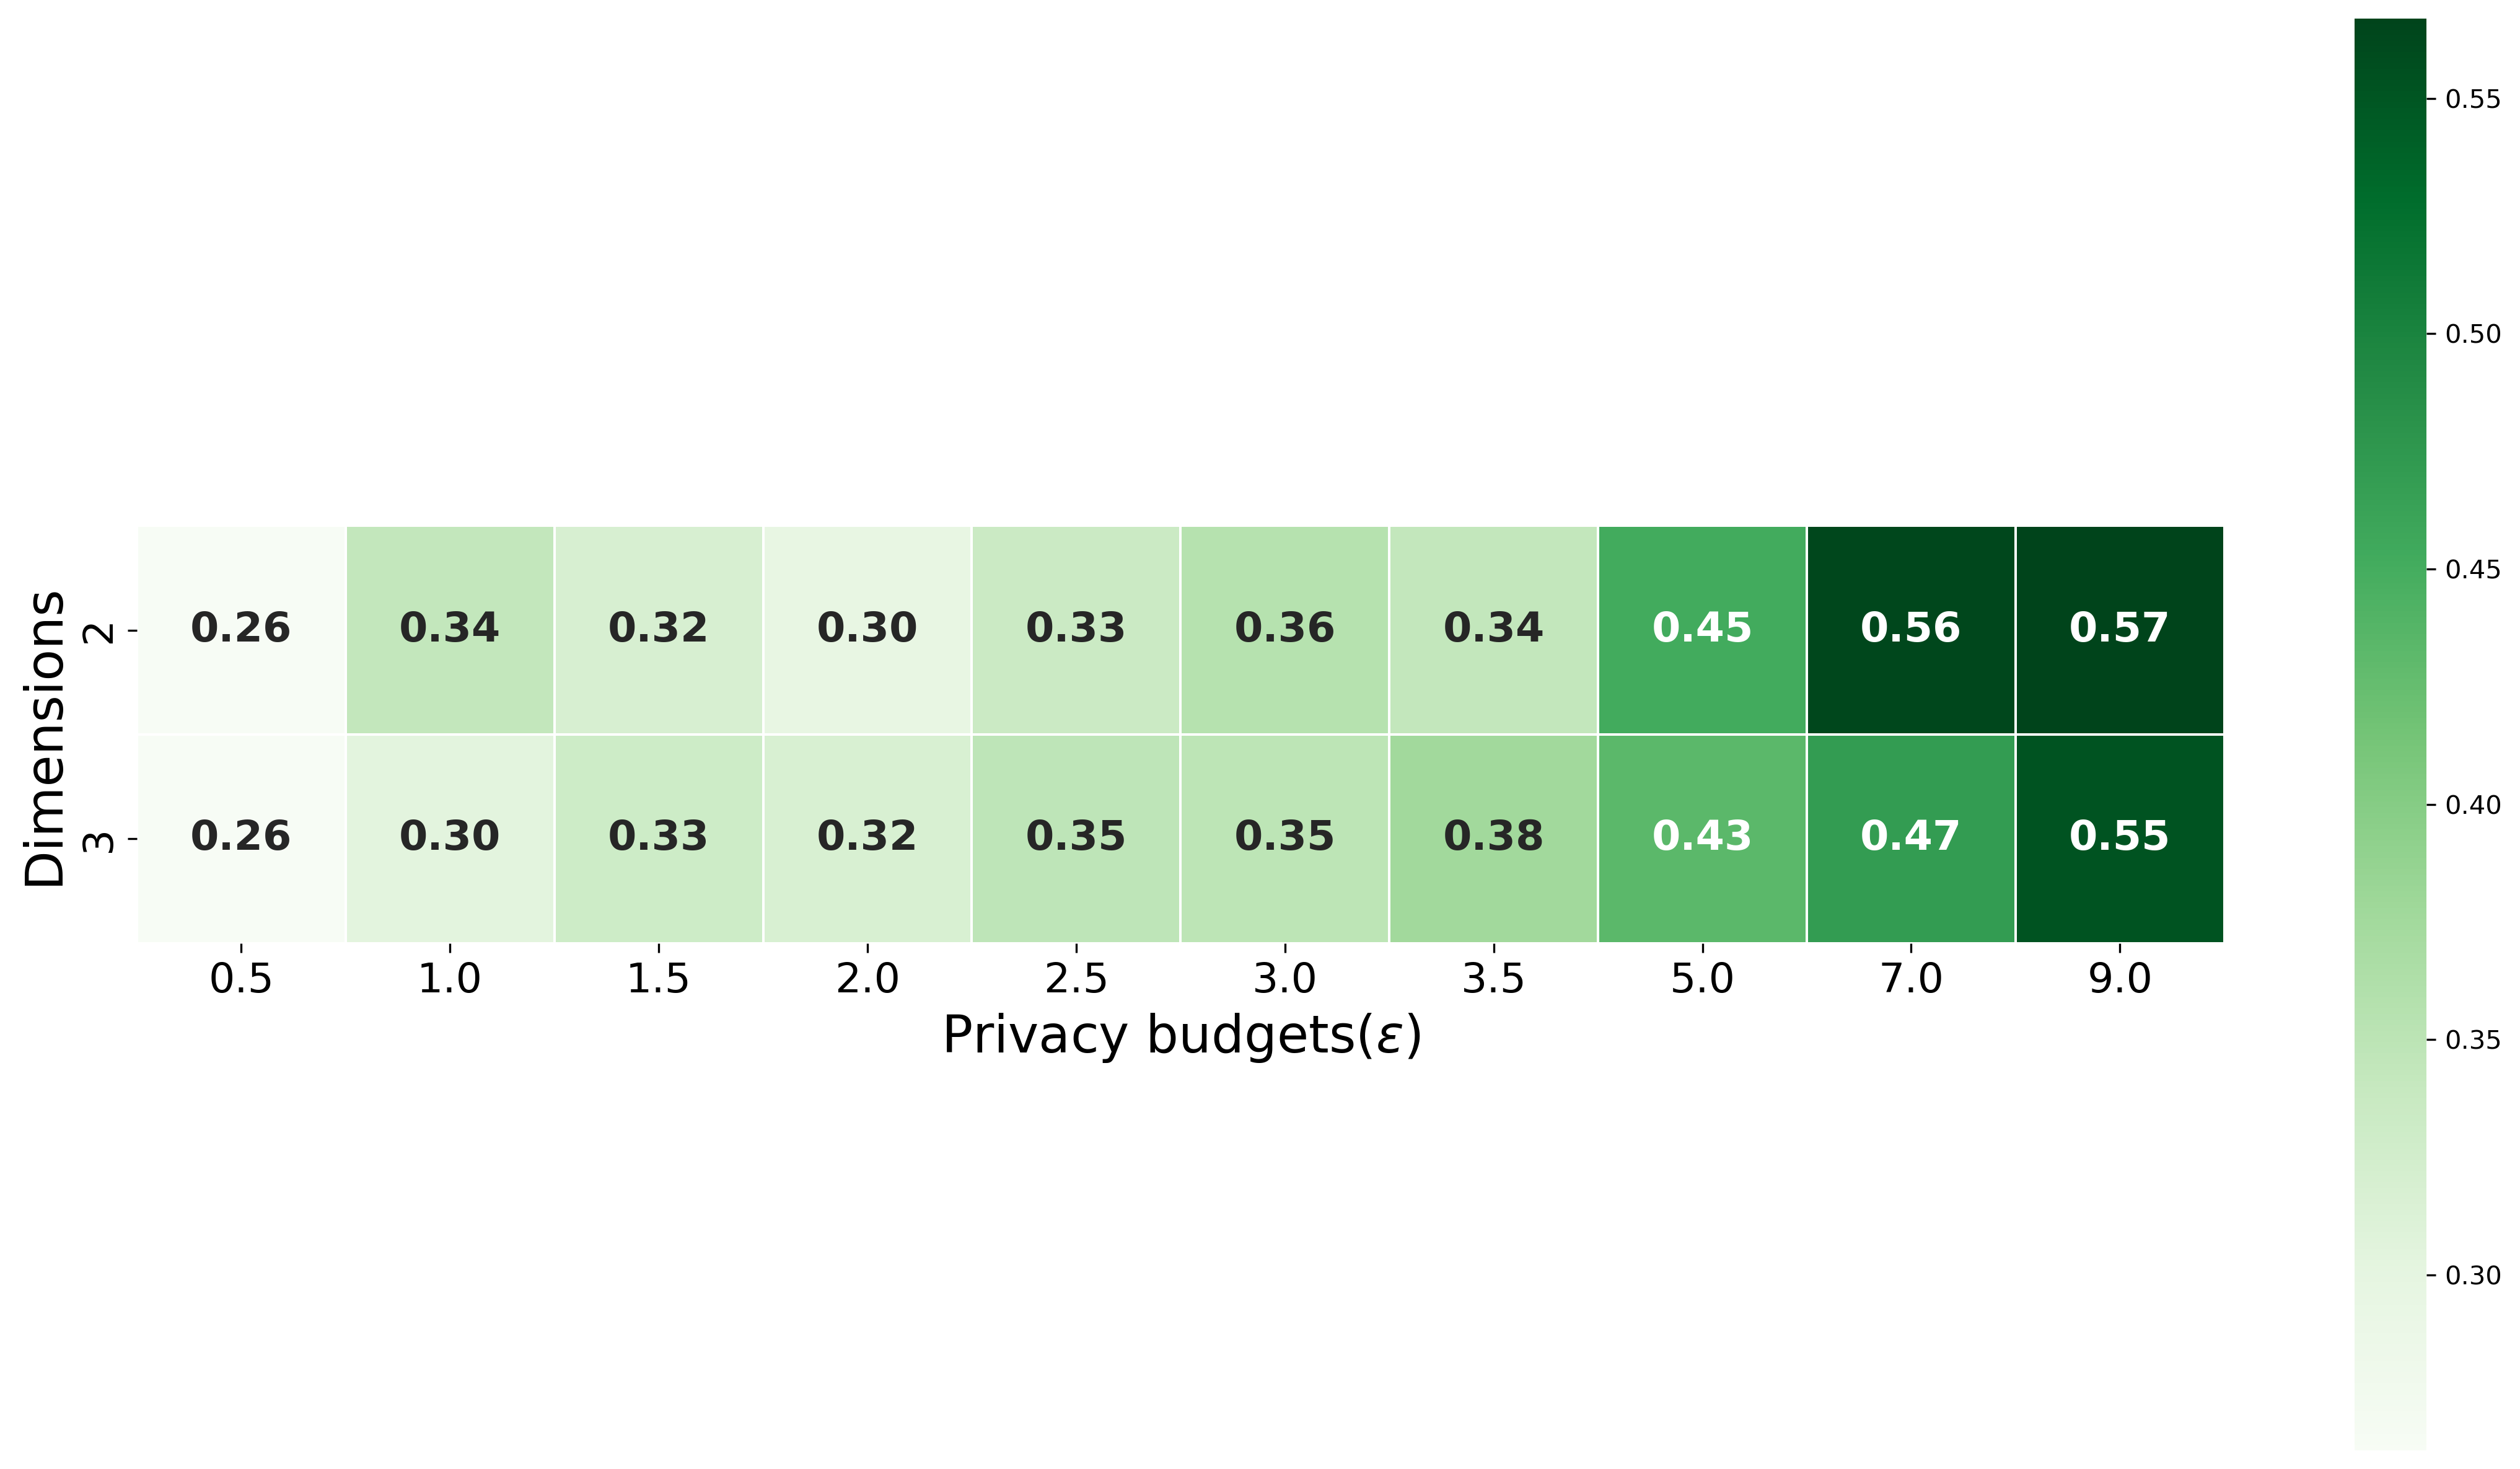
\includegraphics[width=1\textwidth]{Results/nd-laplace/nd-Laplace/line-dataset/tpr.png}
      \label{fig:privacy_tpr_line-dataset_adversial_advantage_kd-laplace}
    \end{subfigure}
    \vfill % vertical space

    \begin{subfigure}[c]{1\textwidth}
      \caption{\textbf{Heatmap TPR for the Piecewise mechanism, per privacy budget \& dimension for line-dataset.}}
      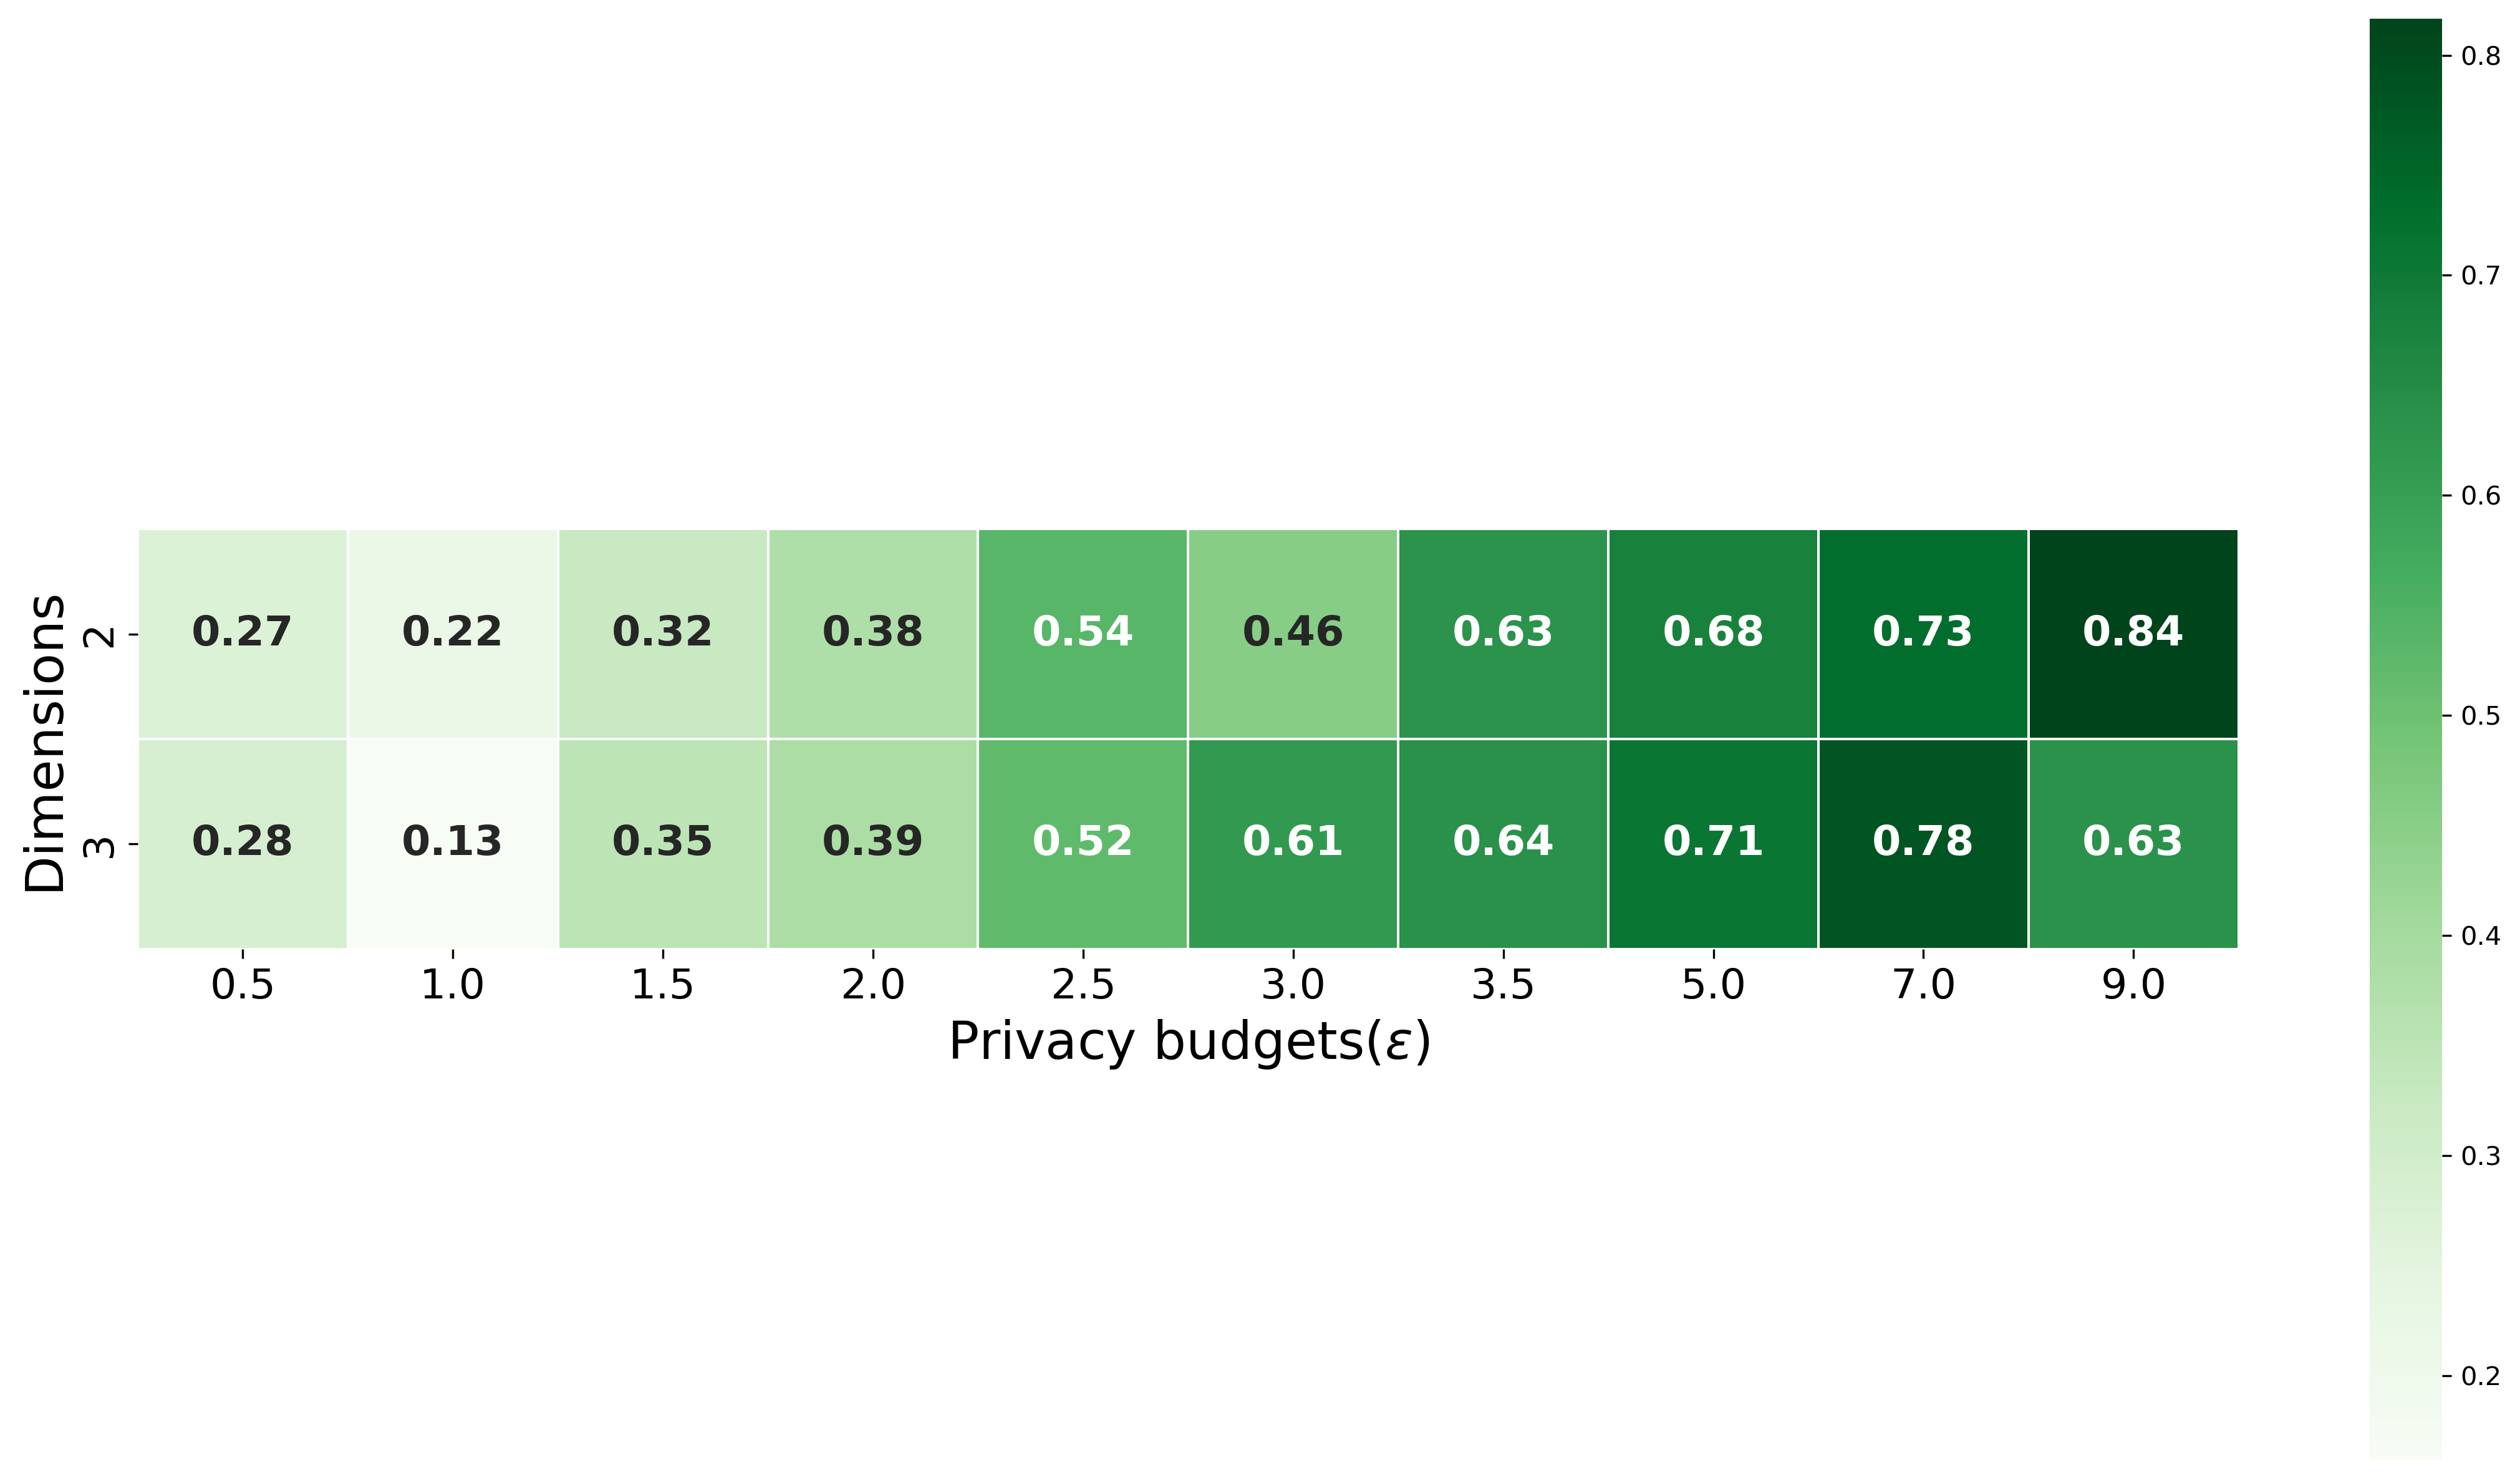
\includegraphics[width=1\textwidth]{Results/nd-laplace/piecewise/line-dataset/tpr.png}
      \label{fig:privacy_tpr_line-dataset_adversial_advantage_piecewise}
    \end{subfigure}
  \end{subfigure}
\end{figure}
Both mechanisms exhibit consistent patterns, and the irregularities previously identified for epsilon values of 0.5 and 1 are not present here. Consequently, it is anticipated that this is a result of a heightened \gls{fpr} in relation to the False/True Negative values.

For the Piecewise mechanism, there is a noticeable increase in membership advantage, approximately 0.2 to 0.3 higher, for epsilon values greater than 2.5. This can be attributed to the mechanism's enhanced utility value for this particular dataset.
\newpage
\subsection{Skewed dataset}
\begin{figure}[H]
  \centering
  \begin{subfigure}[b]{0.85\textwidth}
    \begin{subfigure}[c]{1\textwidth}
      \caption{\textbf{Heatmap showing adversary advantage for the nD-Laplace mechanism, per privacy budget \& dimension for seeds-dataset.}}
      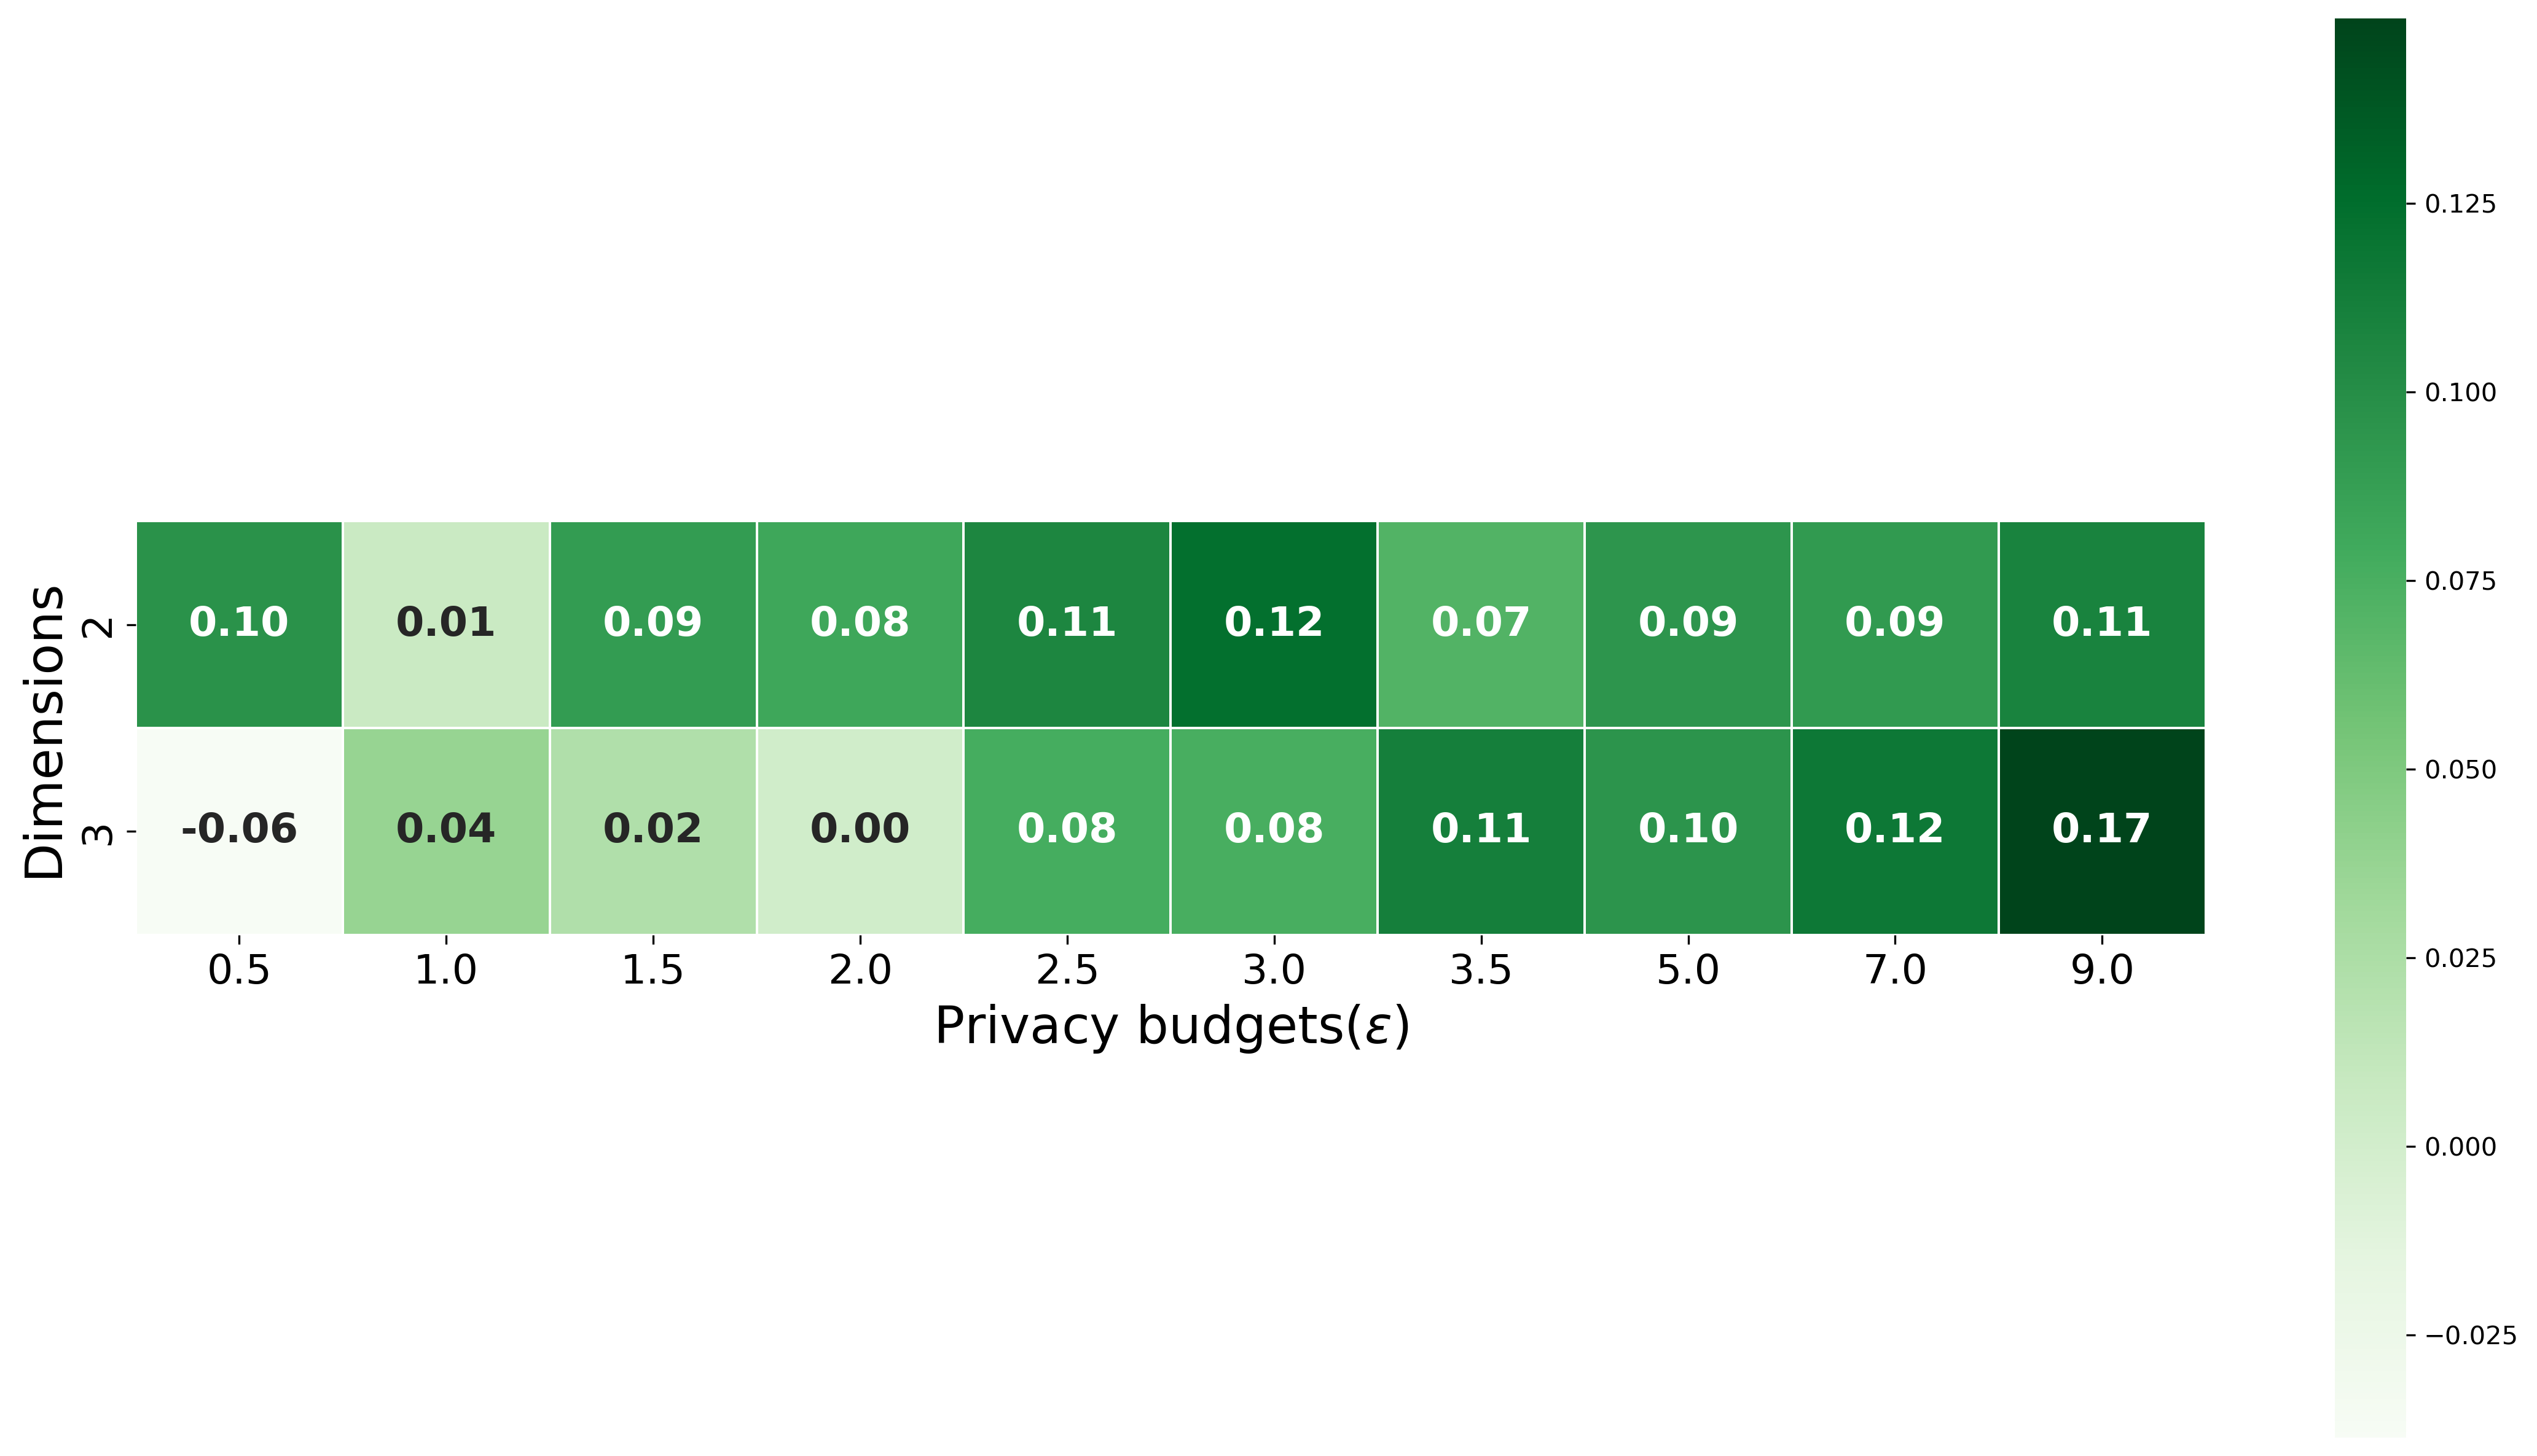
\includegraphics[width=1\textwidth]{Results/nd-laplace/nd-Laplace/skewed-dataset/attack_adv.png}
      \label{fig:privacy_skewed-dataset_adversial_advantage_kd-laplace}
    \end{subfigure}
    \vfill % vertical space

    \begin{subfigure}[c]{1\textwidth}
      \caption{\textbf{Heatmap showing adversary advantage for the Piecewise mechanism, per privacy budget \& dimension for seeds-dataset.}}
      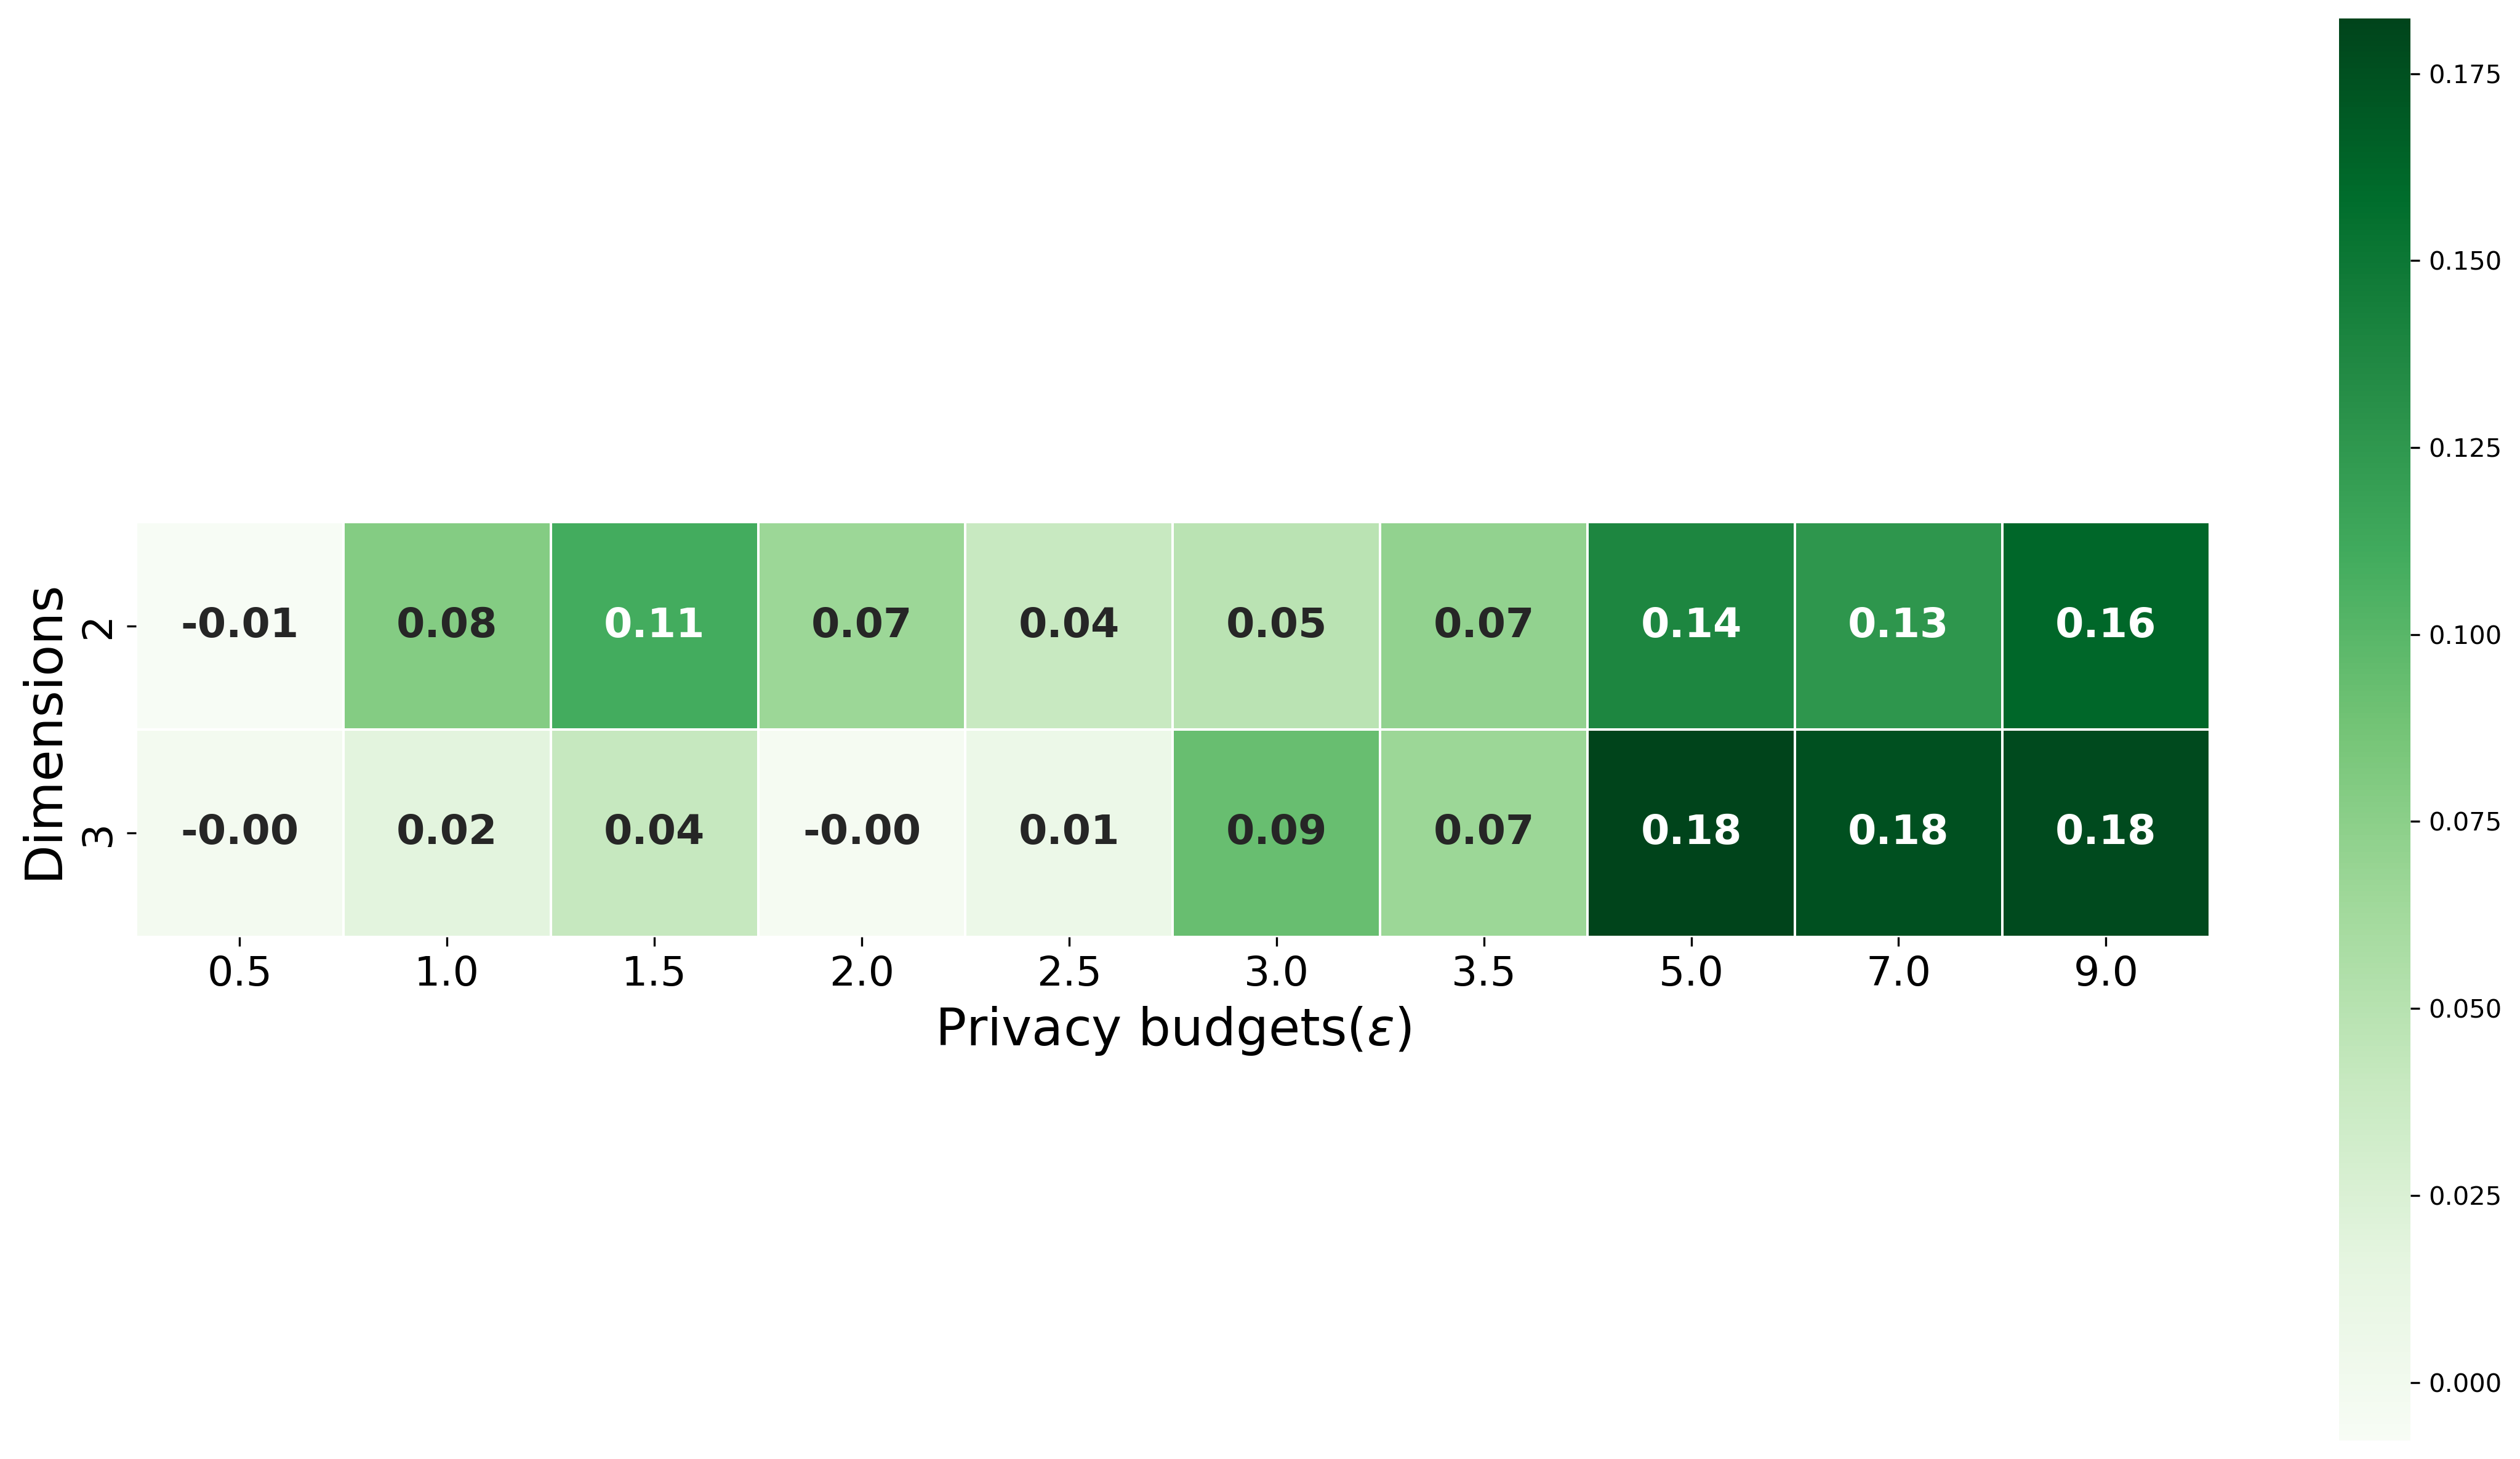
\includegraphics[width=1\textwidth]{Results/nd-laplace/piecewise/skewed-dataset/attack_adv.png}
      \label{fig:privacy_skewed-dataset_adversial_advantage_piecewise}
    \end{subfigure}
  \end{subfigure}
\end{figure}

The nD-Laplace mechanism exhibits a modest correlation with the privacy budget for 3-dimensional data. However, for the 2-dimensional data, there is minimal variation in the membership advantage. Within the heatmap, the privacy budget of 1.5 stands out due to its lighter shade, but the difference is still marginal (0.01) compared to the rest of the heatmap.

In contrast, the Piecewise mechanism displays a more pronounced pattern. For 2-dimensional data, the trend aligns with the utility, especially for higher privacy budgets where the \gls{ami} exceeded 0.85. For 3-dimensional data, it is particularly evident that the privacy budgets ranging from 0.5 to 1.5 exhibit minimal membership advantage. This observation is consistent with the \gls{ami} values, which are approximately 0.00.

The low membership advantage for the nD-Laplace mechanism is noteworthy, given its high \gls{ami} score. This is reflected in the membership advantage for privacy budgets of 7 and 9, but not for other values. The Piecewise mechanism offers a clearer picture, as the elevated \gls{ami} values correlate with higher membership advantages. In addition to these shifts, the results for 3-dimensional data and lower privacy budgets are also of interest. On the subsequent page, the \gls{tpr} is presented to determine if similar observations can be made.
\newpage

\begin{figure}[H]
  \centering
  \begin{subfigure}[b]{0.9\textwidth}
    \begin{subfigure}[c]{1\textwidth}
      \caption{\textbf{Heatmap TPR for the nD-Laplace mechanism, per privacy budget \& dimension for skewed-dataset.}}
      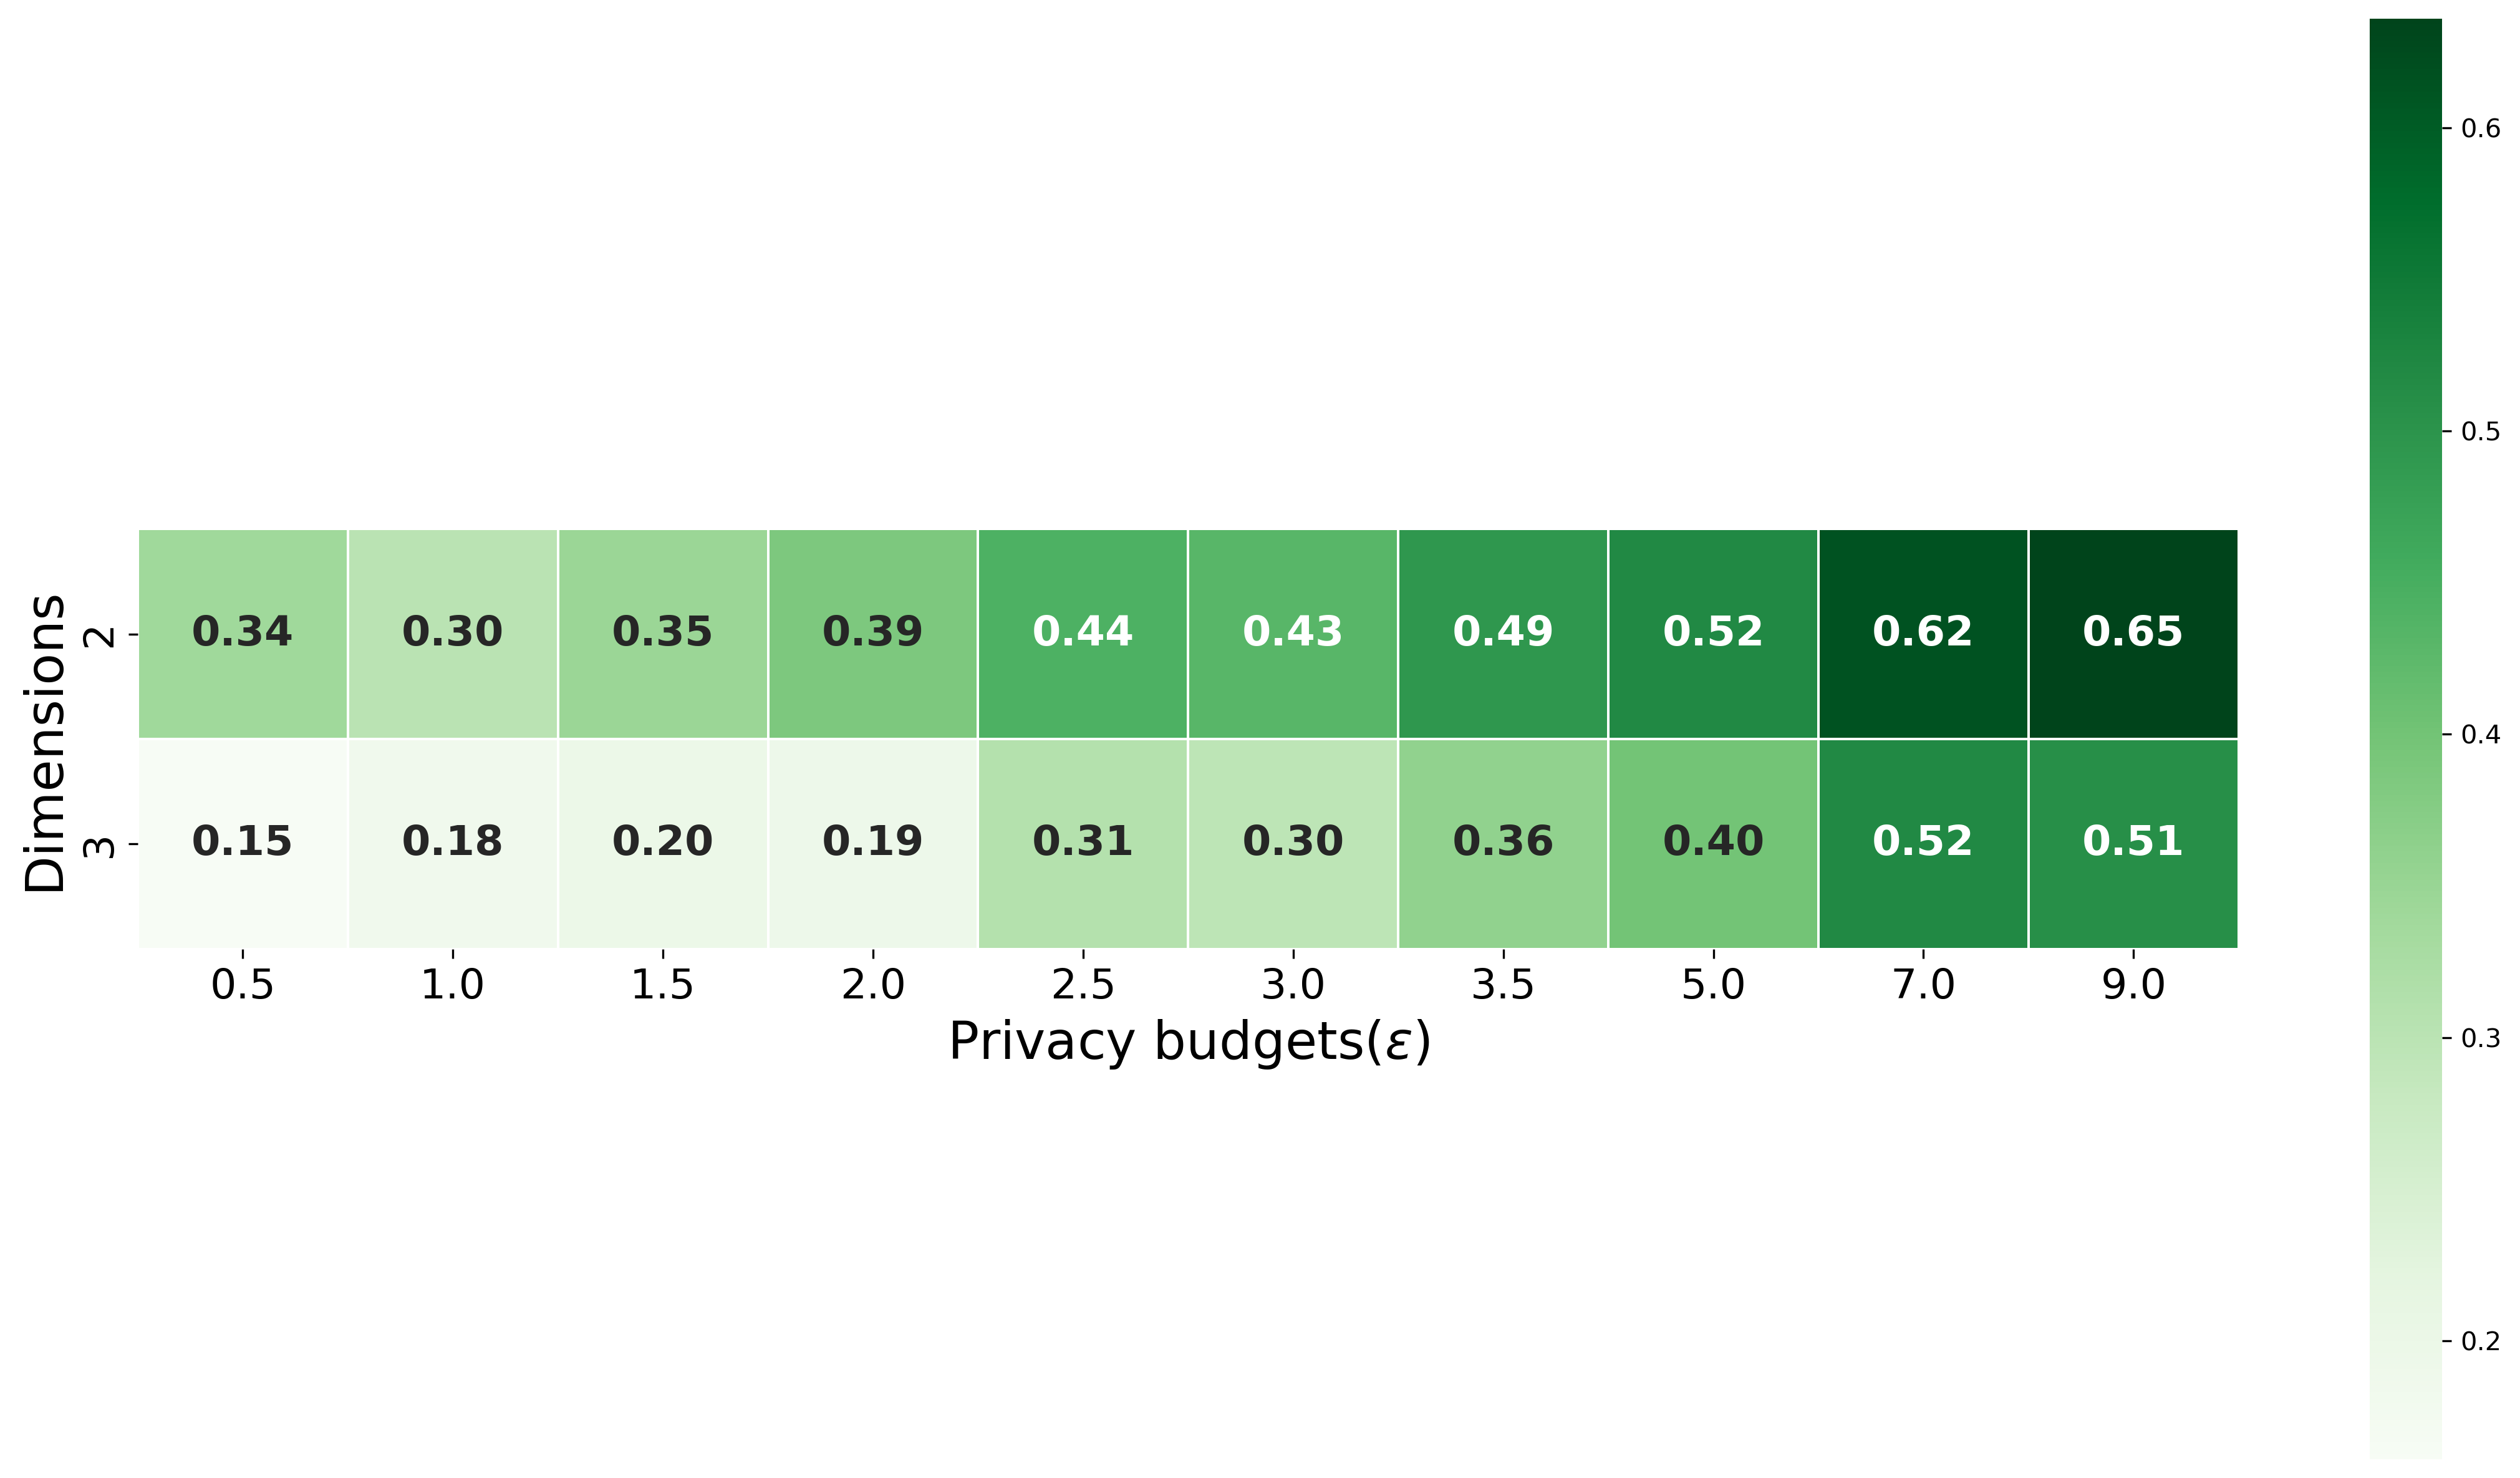
\includegraphics[width=1\textwidth]{Results/nd-laplace/nd-Laplace/skewed-dataset/tpr.png}
      \label{fig:privacy_tpr_skewed-dataset_adversial_advantage_kd-laplace}
    \end{subfigure}
    \vfill % vertical space

    \begin{subfigure}[c]{1\textwidth}
      \caption{\textbf{Heatmap TPR for the Piecewise mechanism, per privacy budget \& dimension for skewed-dataset.}}
      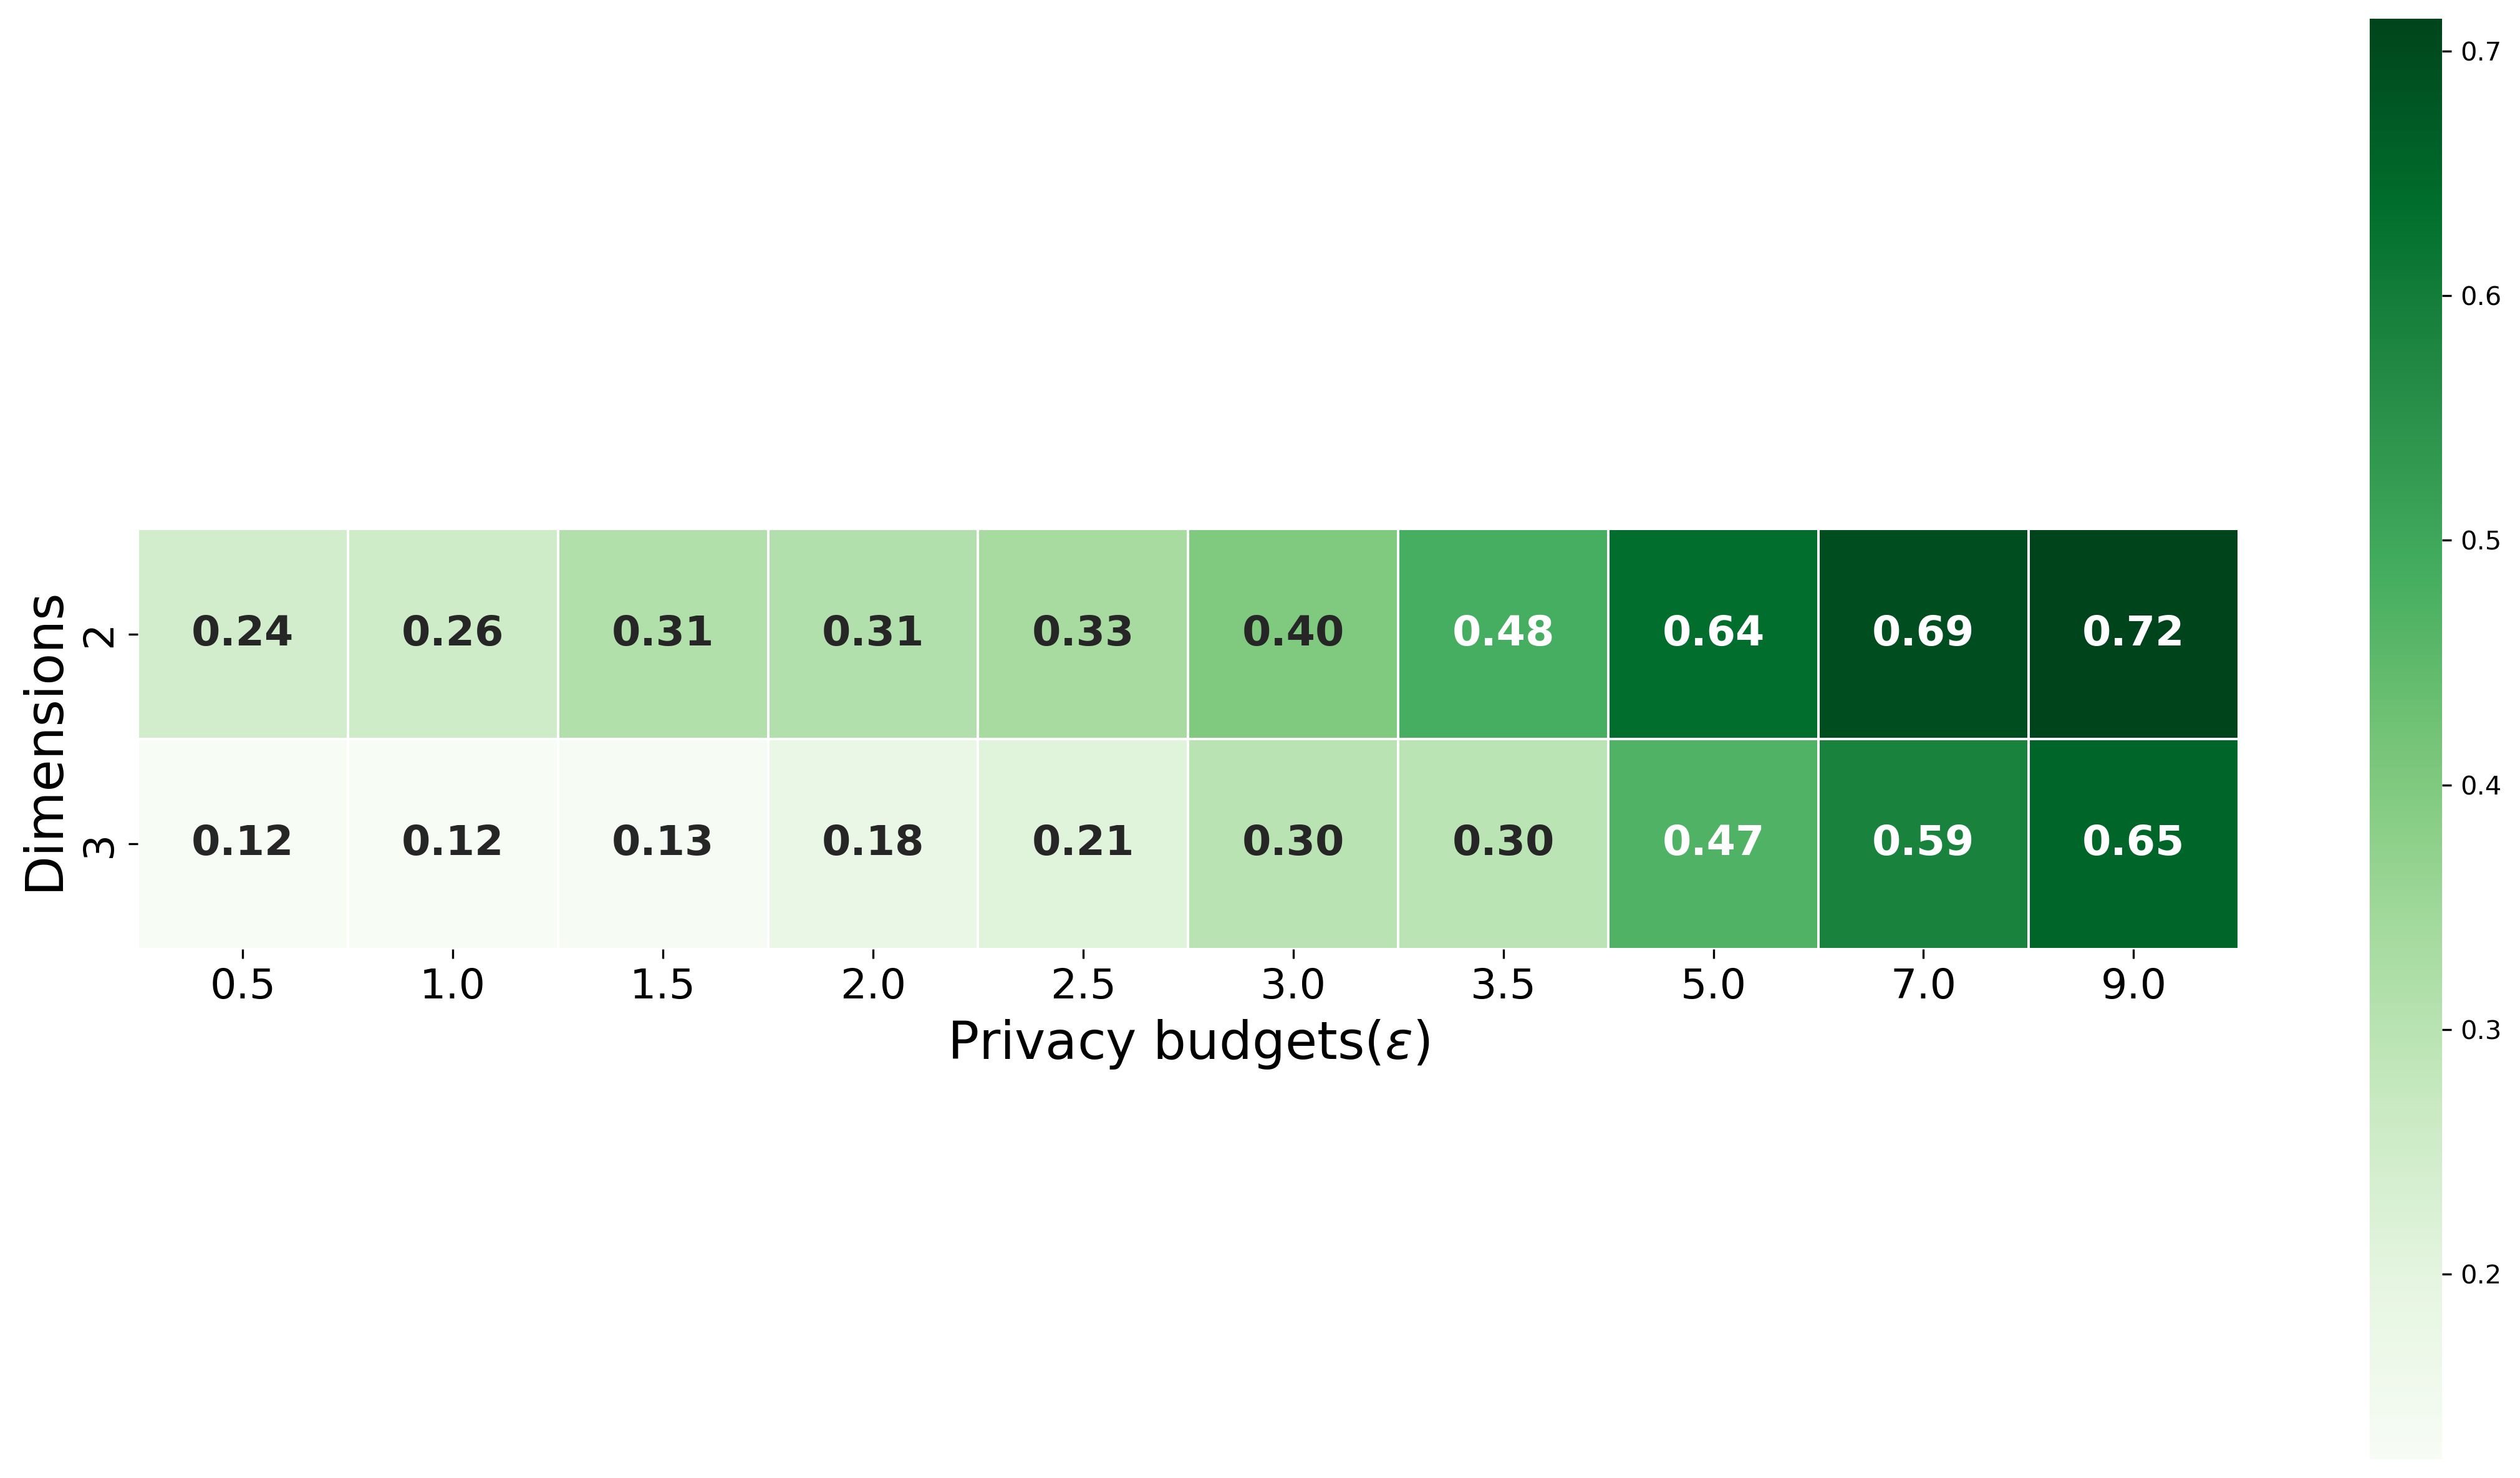
\includegraphics[width=1\textwidth]{Results/nd-laplace/piecewise/skewed-dataset/tpr.png}
      \label{fig:privacy_tpr_skewed-dataset_adversial_advantage_piecewise}
    \end{subfigure}
  \end{subfigure}
\end{figure}
Both mechanisms exhibit consistent values, yet they reveal nearly all the information.

For the nD-Laplace mechanism, a high \gls{ami} is observed across numerous privacy budgets. However, for the more constrained privacy budgets, the \gls{ami} is notably lower, suggesting that the \gls{tpr} should similarly be reduced.

Conversely, the Piecewise mechanism demonstrates a less favorable performance. This mechanism consistently registers a significantly lower \gls{ami} (below 0.5) for all privacy budgets up to 5.
%\todo[inline]{Why is the TPR so freaking high?}

\subsection{Mechanism comparison}
In this section, we compare the different mechanisms for each dataset.
For this purpose, we also include all the different variants of nD-Laplace to see if there is a difference between them.
So, instead of comparing the mechanisms based on the number of dimensions, we compare them on the average scores for all dimensions per mechanism.
We are most interested in the utility and performance, and to compare them, we only show the \gls{ami} and adversary advantage scores.
\newpage
\begin{figure}[H]
  \centering
  \begin{subfigure}{0.30\textwidth}
    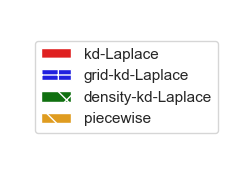
\includegraphics[width=\textwidth]{Results/kd-laplace/ami_bar_comparison_legend.png}
  \end{subfigure}
  \begin{subfigure}{1\textwidth}
    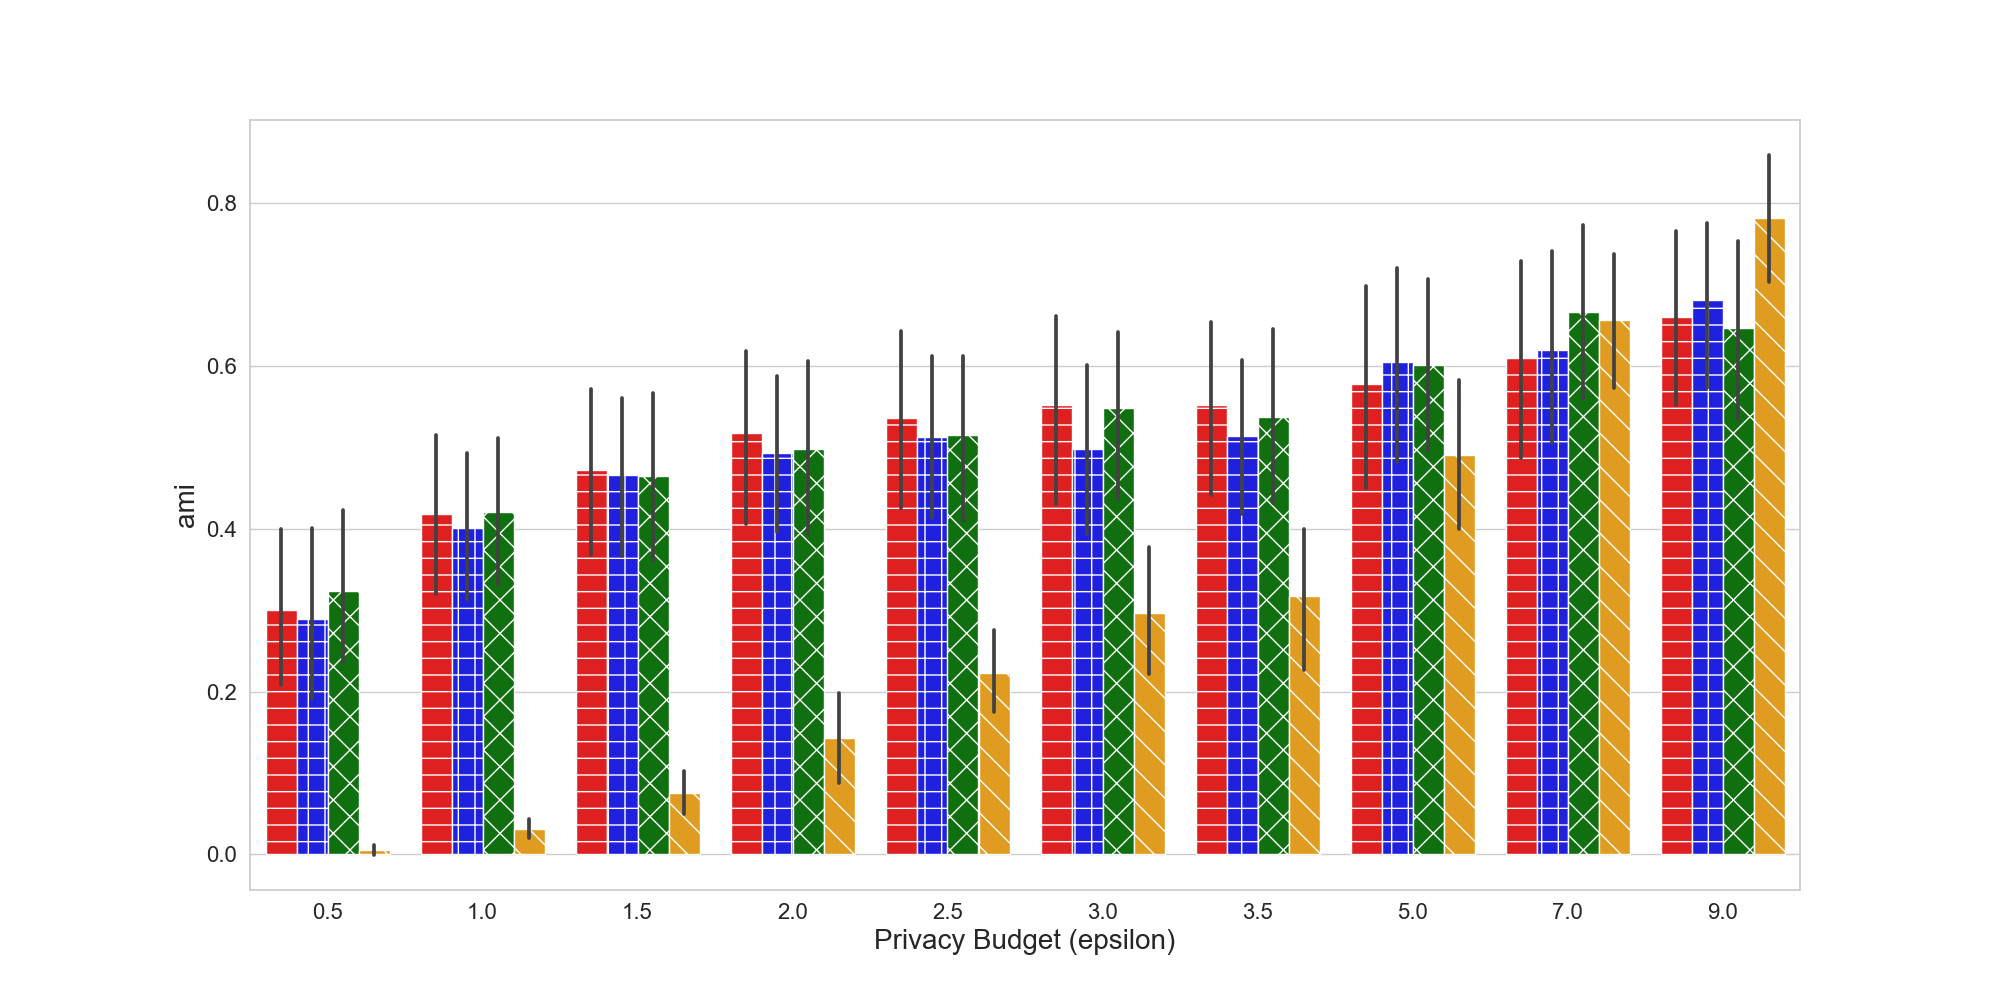
\includegraphics[width=1\textwidth]{Results/nd-laplace/ami_seeds-dataset_comparison.png}
  \end{subfigure}
  \begin{subfigure}{1\textwidth}
    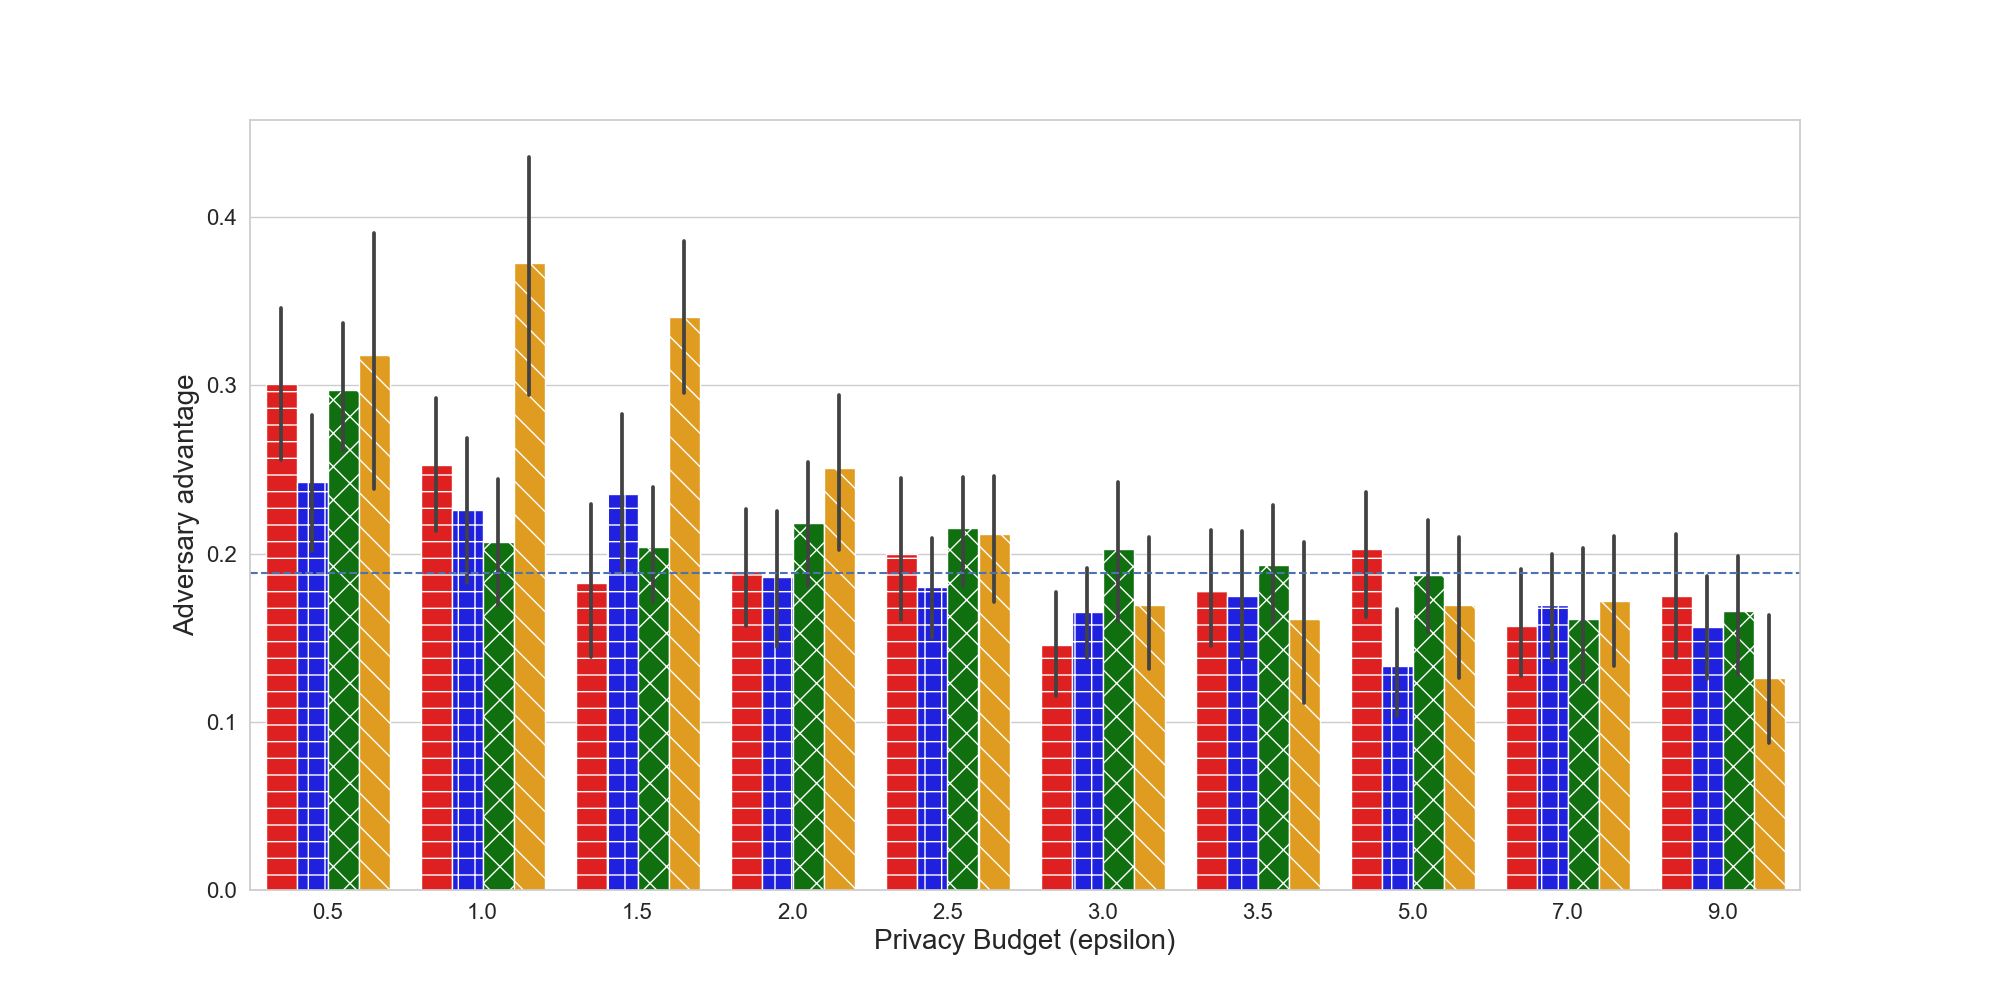
\includegraphics[width=1\textwidth]{Results/nd-laplace/attack_adv_seeds-dataset_comparison.png}
  \end{subfigure}
  \caption{Average AMI (top) and Adversary Advantage (bottom) comparison for each mechanism for seeds-dataset (8 dimensions).}
  \label{fig:utility_seeds-dataset_comparison_nd_plot}
\end{figure}
The presented plot illustrates the \gls{ami} values for various configurations of the nD-Laplace and Piecewise mechanisms. Notably, the Piecewise mechanism yields a lower \gls{ami} compared to nD-Laplace. Among the three configurations, there isn't a singular mechanism that consistently surpasses the others; their performance is contingent upon specific privacy budget values. Although the Piecewise mechanism demonstrates a commendable membership advantage, one must consider the anomalies in the privacy budgets between 0.5 and 1.5. Outside of this range, the Piecewise mechanism provides only a slight enhancement in privacy.
\newpage


\begin{figure}[H]
  \centering
  \begin{subfigure}{0.30\textwidth}
    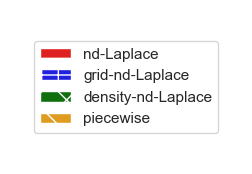
\includegraphics[width=\textwidth]{Results/nd-laplace/ami_bar_comparison_legend.png}
  \end{subfigure}
  \begin{subfigure}{1\textwidth}
    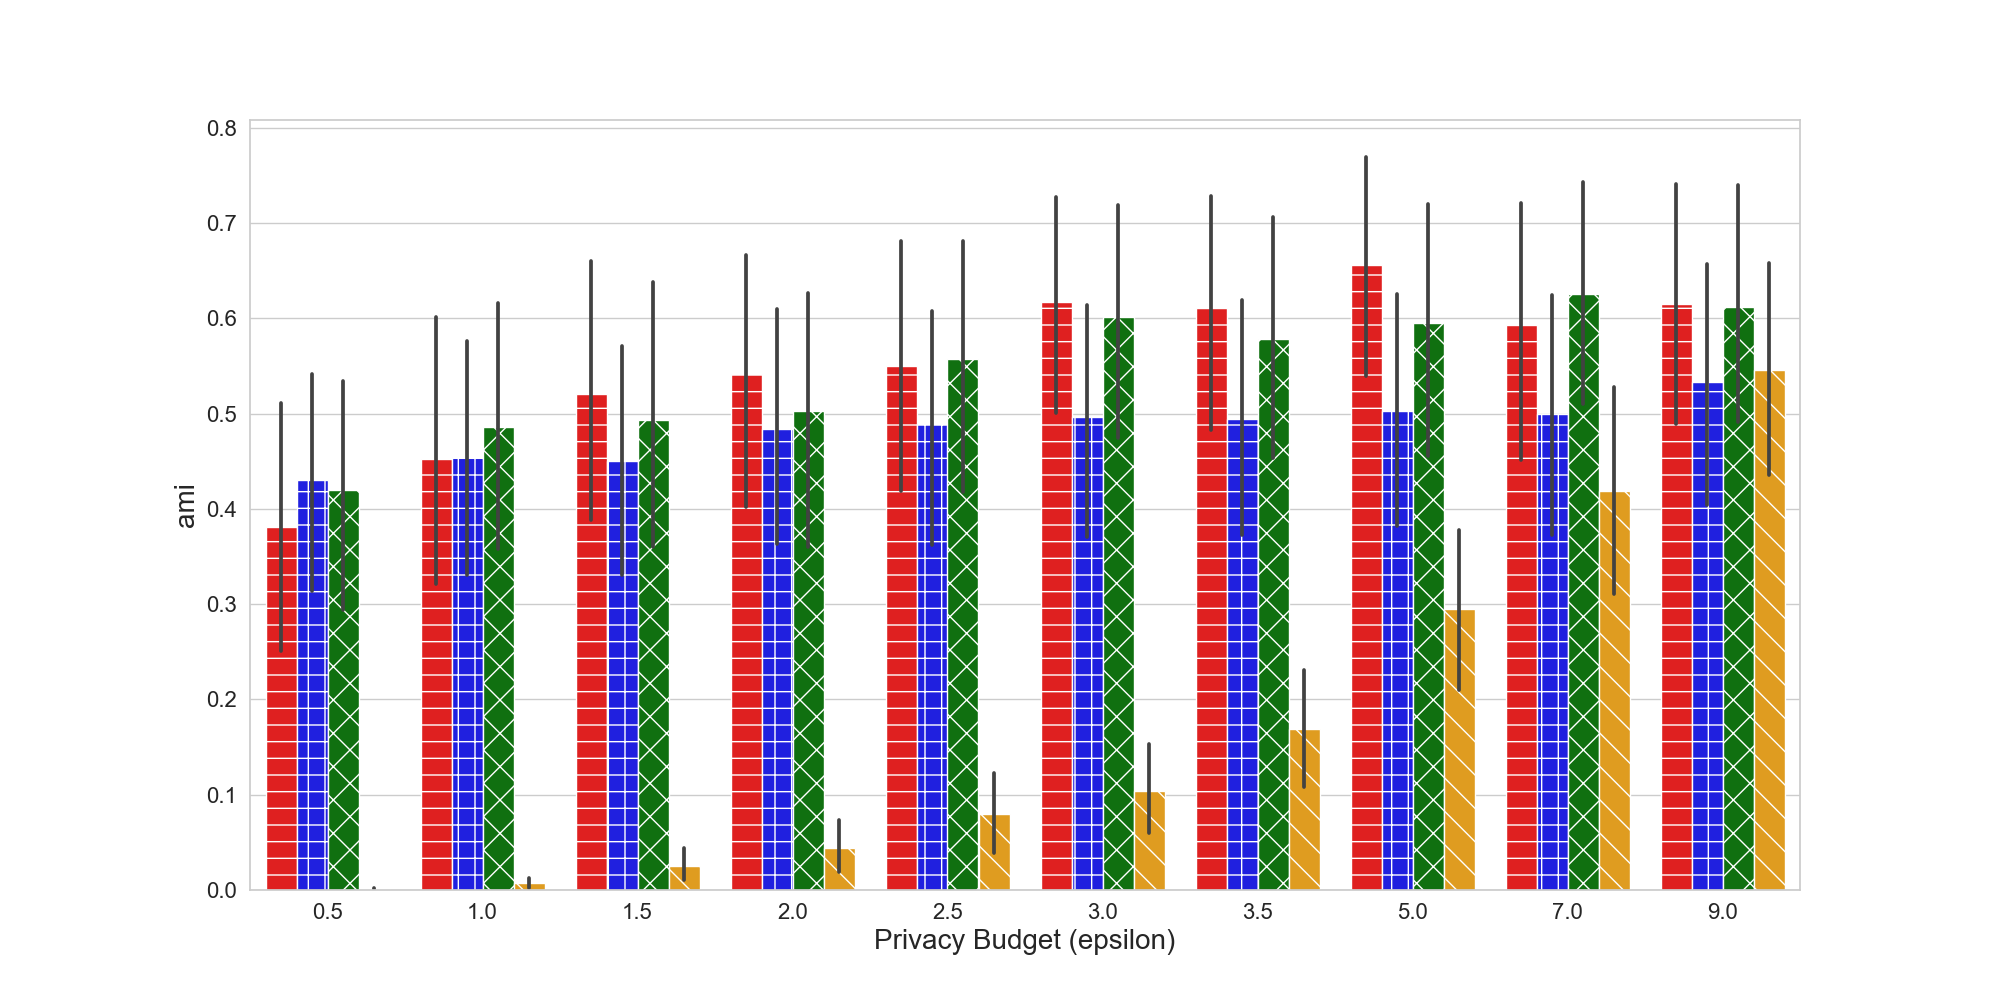
\includegraphics[width=1\textwidth]{Results/nd-laplace/ami_heart-dataset_comparison.png}
  \end{subfigure}
  \begin{subfigure}{1\textwidth}
    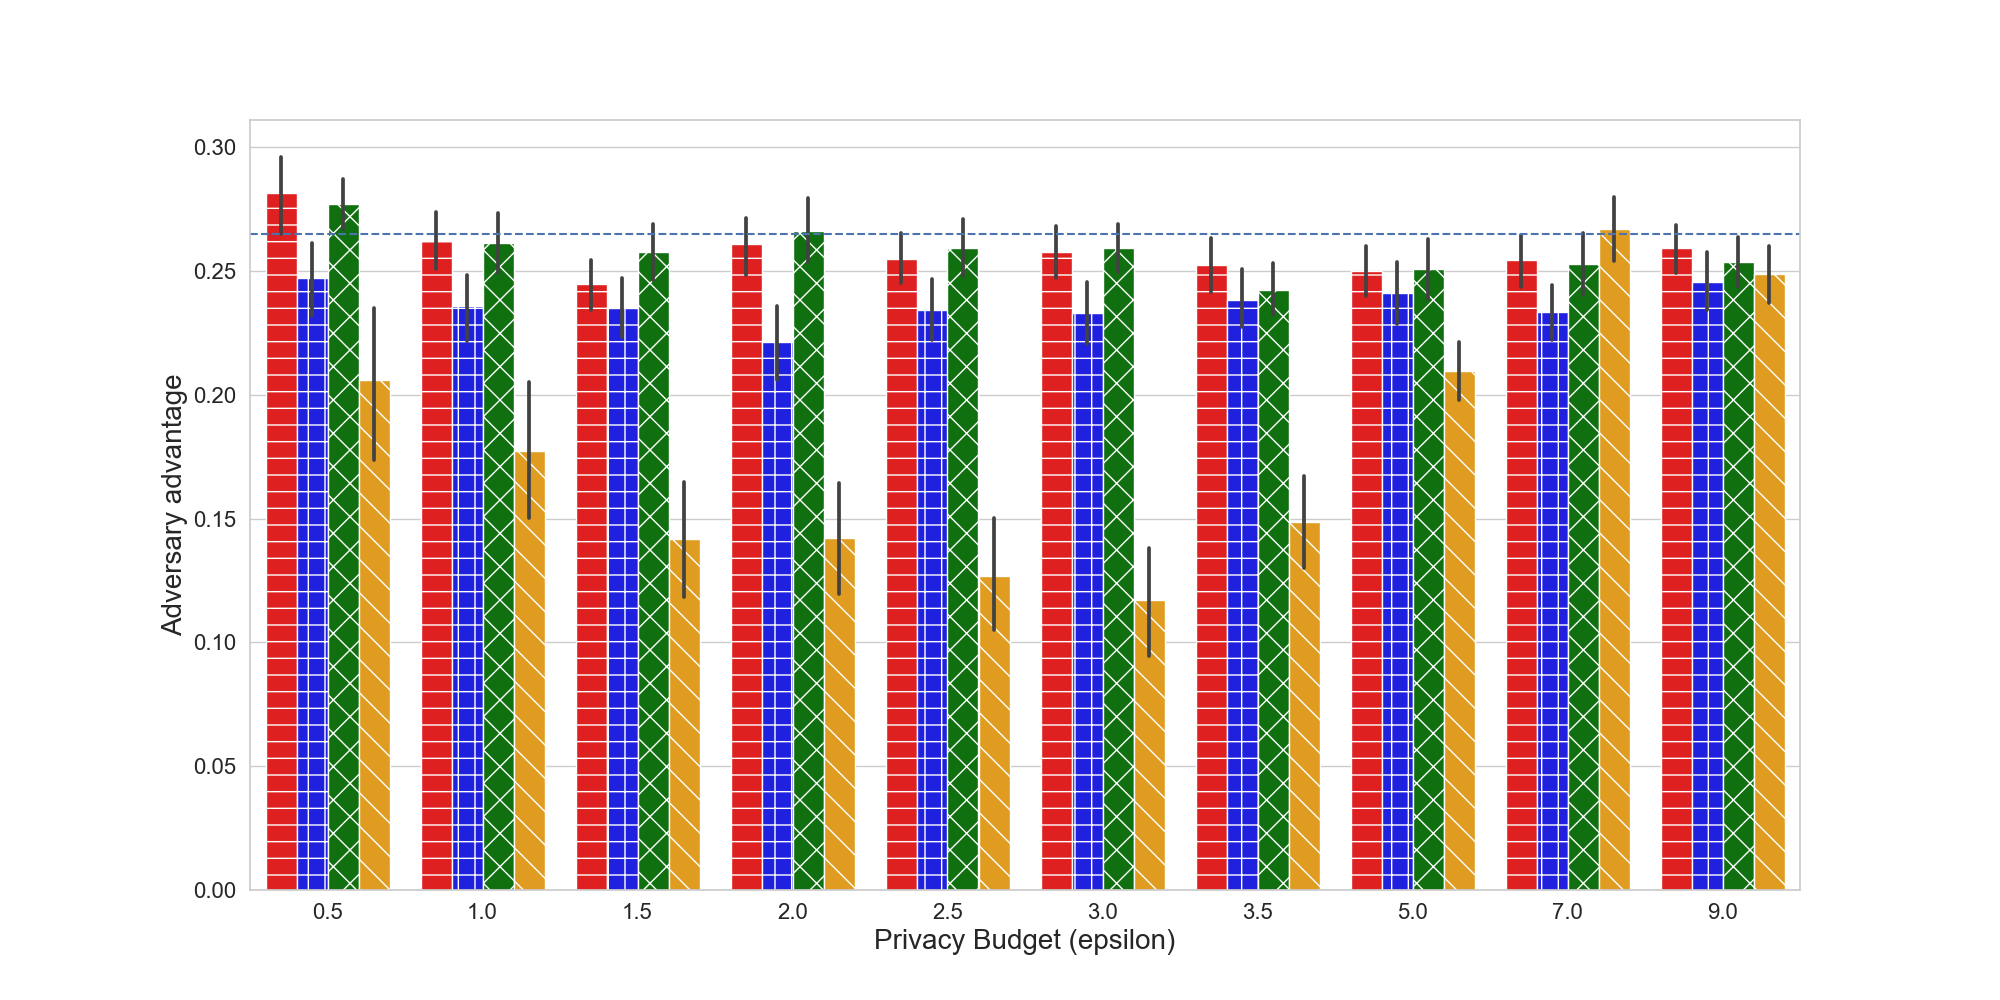
\includegraphics[width=1\textwidth]{Results/nd-laplace/attack_adv_heart-dataset_comparison.png}
  \end{subfigure}
  \caption{Average AMI (top) and Adversary Advantage (bottom) comparison for each mechanism for heart-dataset (10 dimensions).}
  \label{fig:utility_heart-dataset_comparison_nd_plot}
\end{figure}
Building upon the cluster and utility plots discussed in previous sections, the heart-dataset consistently exhibits elevated \gls{ami} values. Both density-nD-Laplace and nD-Laplace mechanisms achieve the highest scores, whereas the grid-based variant remains relatively constant. Among the three configurations, the grid-nD-Laplace offers the most robust privacy.

The membership advantage of the Piecewise mechanism is closely tied to its \gls{ami} performance. As a result, it registers low values across all epsilons but aligns closely with privacy budgets 7 and 9. Notably, all mechanisms, with the exception of nD-Laplace and density-nD-Laplace, fall below the baseline value.

For the nD-Laplace mechanism, a significant portion of data deviates from the original domain $X$ when the privacy budget is set at 0.5. This deviation leads the classifier to train on inaccurate data, resulting in overfitting since it lacks generalization to the unaltered data (test dataset) as elucidated by \citep{shokri_membership_2017}. This phenomenon makes it more discernible to distinguish between member and non-member data. A similar trend is observed with the Piecewise mechanism, albeit to a lesser degree. The Piecewise mechanism more adeptly conforms to the shape of the original data, as seen in (\ref{fig:evaluate-optics-seeds-dataset-2d-9eps}), while nD-Laplace disperses the data uniformly in all directions.
% \todo[inline]{Examine the behavior of density-remapping as well.}
\newpage

\subsection{Shape datasets}

\begin{figure}[H]
  \centering
  \begin{subfigure}{0.30\textwidth}
    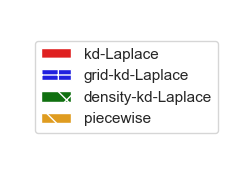
\includegraphics[width=\textwidth]{Results/kd-laplace/ami_bar_comparison_legend.png}
  \end{subfigure}
  \begin{subfigure}{1\textwidth}
    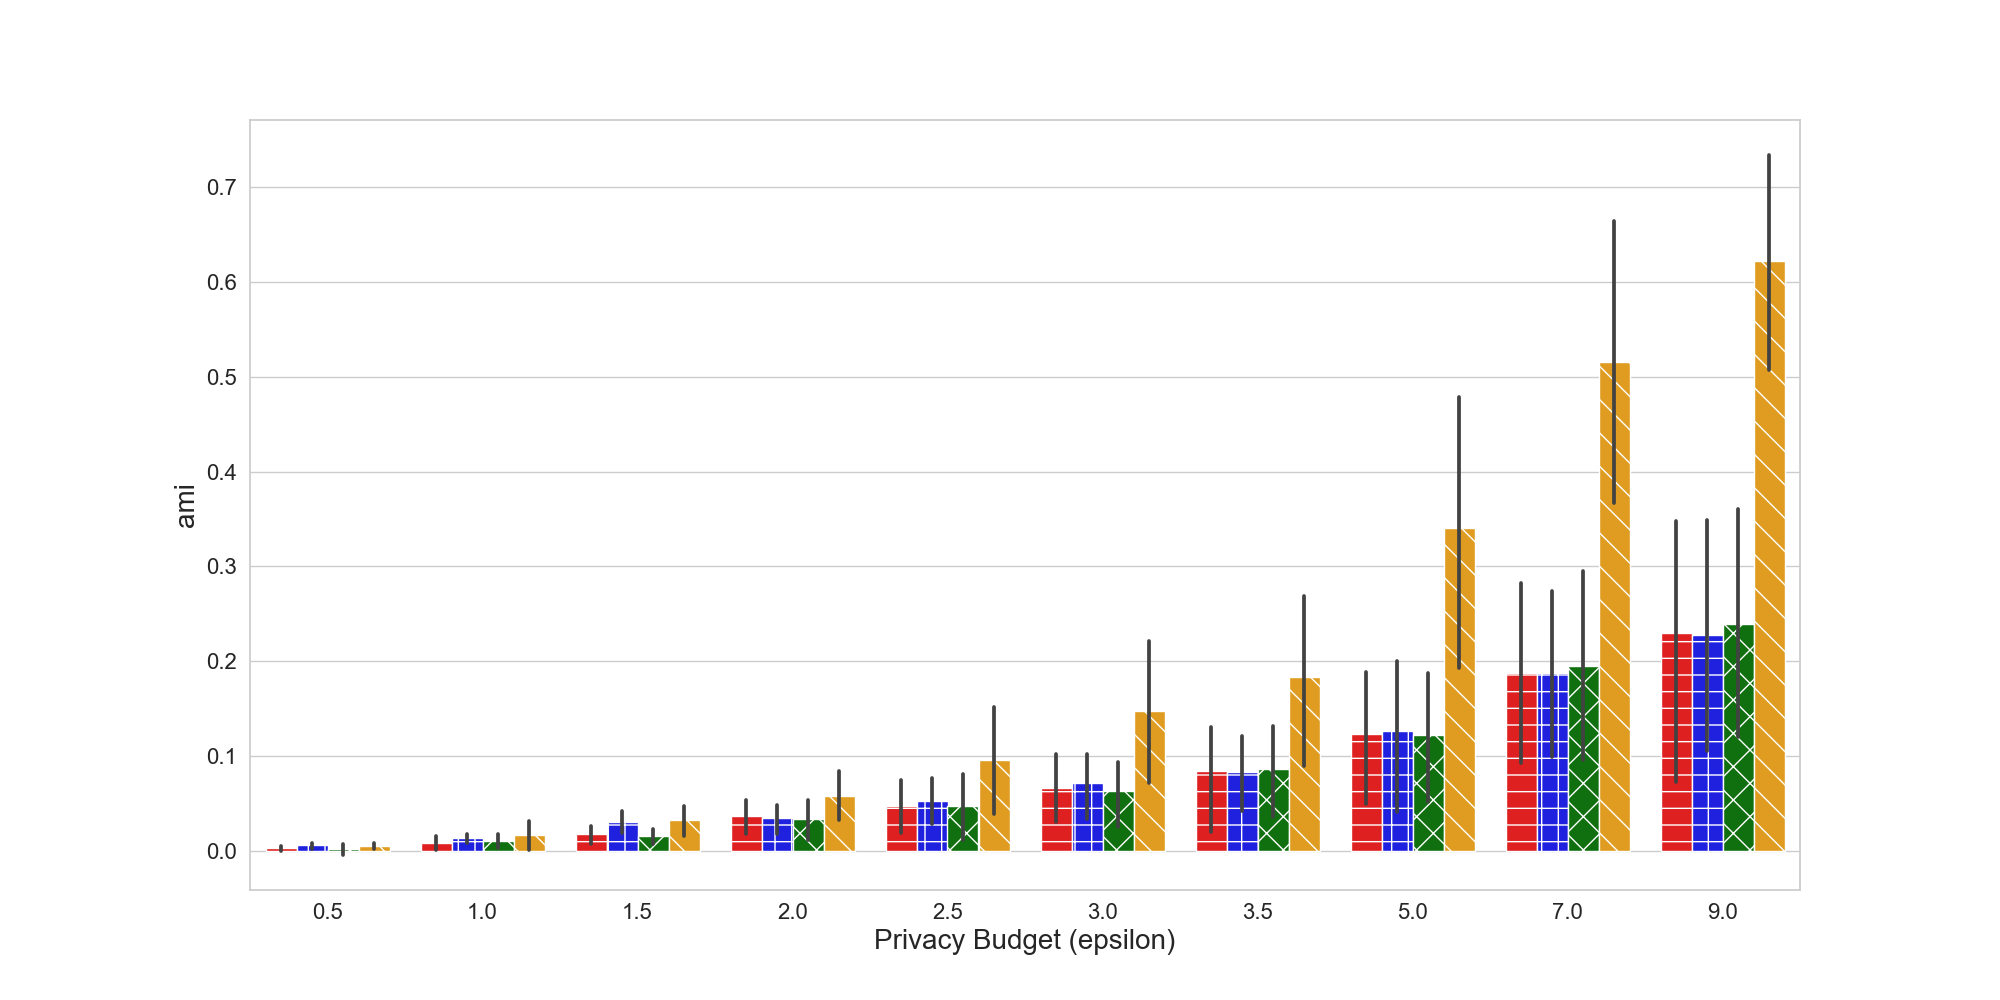
\includegraphics[width=1\textwidth]{Results/nd-laplace/ami_circle-dataset_comparison.png}
  \end{subfigure}
  \begin{subfigure}{1\textwidth}
    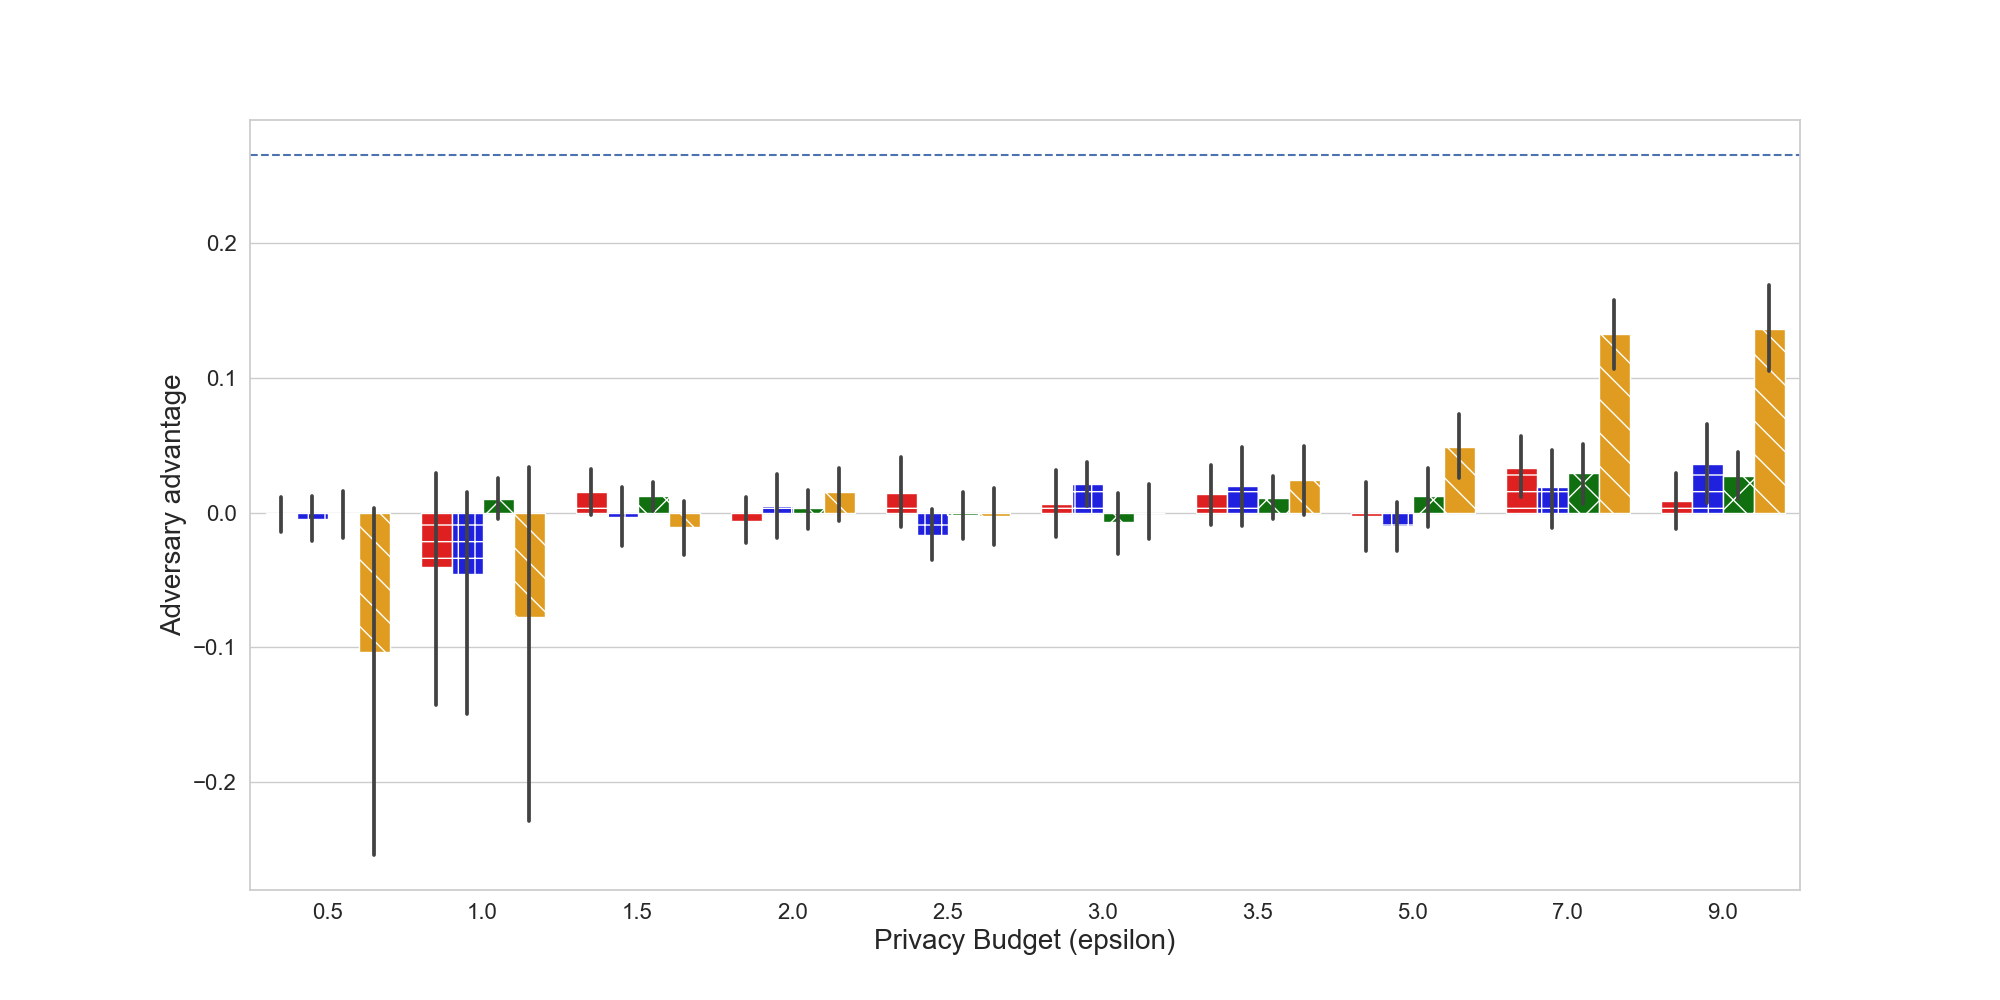
\includegraphics[width=1\textwidth]{Results/nd-laplace/attack_adv_circle-dataset_comparison.png}
  \end{subfigure}
  \caption{Average AMI (top) and Adversary Advantage (bottom) comparison for each mechanism for circle-dataset (3 dimensions).}
  \label{fig:utility_circle-dataset_comparison_nd_plot}
\end{figure}

The observed trend for the seeds-dataset and heart-dataset is inversed, with the Piecewise mechanism emerging as the more favorable option. For the nD-Laplace mechanism, the utility remains notably low, and its variants do not present any significant enhancement in this regard. As a result, while the privacy levels are elevated for nD-Laplace, the Piecewise mechanism still provides superior privacy, especially for the lower privacy budgets. Predictably, the Piecewise mechanism exhibits reduced privacy (manifested as a higher advantage) for the more generous privacy budgets.
\newpage

\begin{figure}[H]
  \centering
  \begin{subfigure}{0.30\textwidth}
    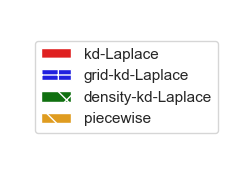
\includegraphics[width=\textwidth]{Results/kd-laplace/ami_bar_comparison_legend.png}
  \end{subfigure}
  \begin{subfigure}{1\textwidth}
    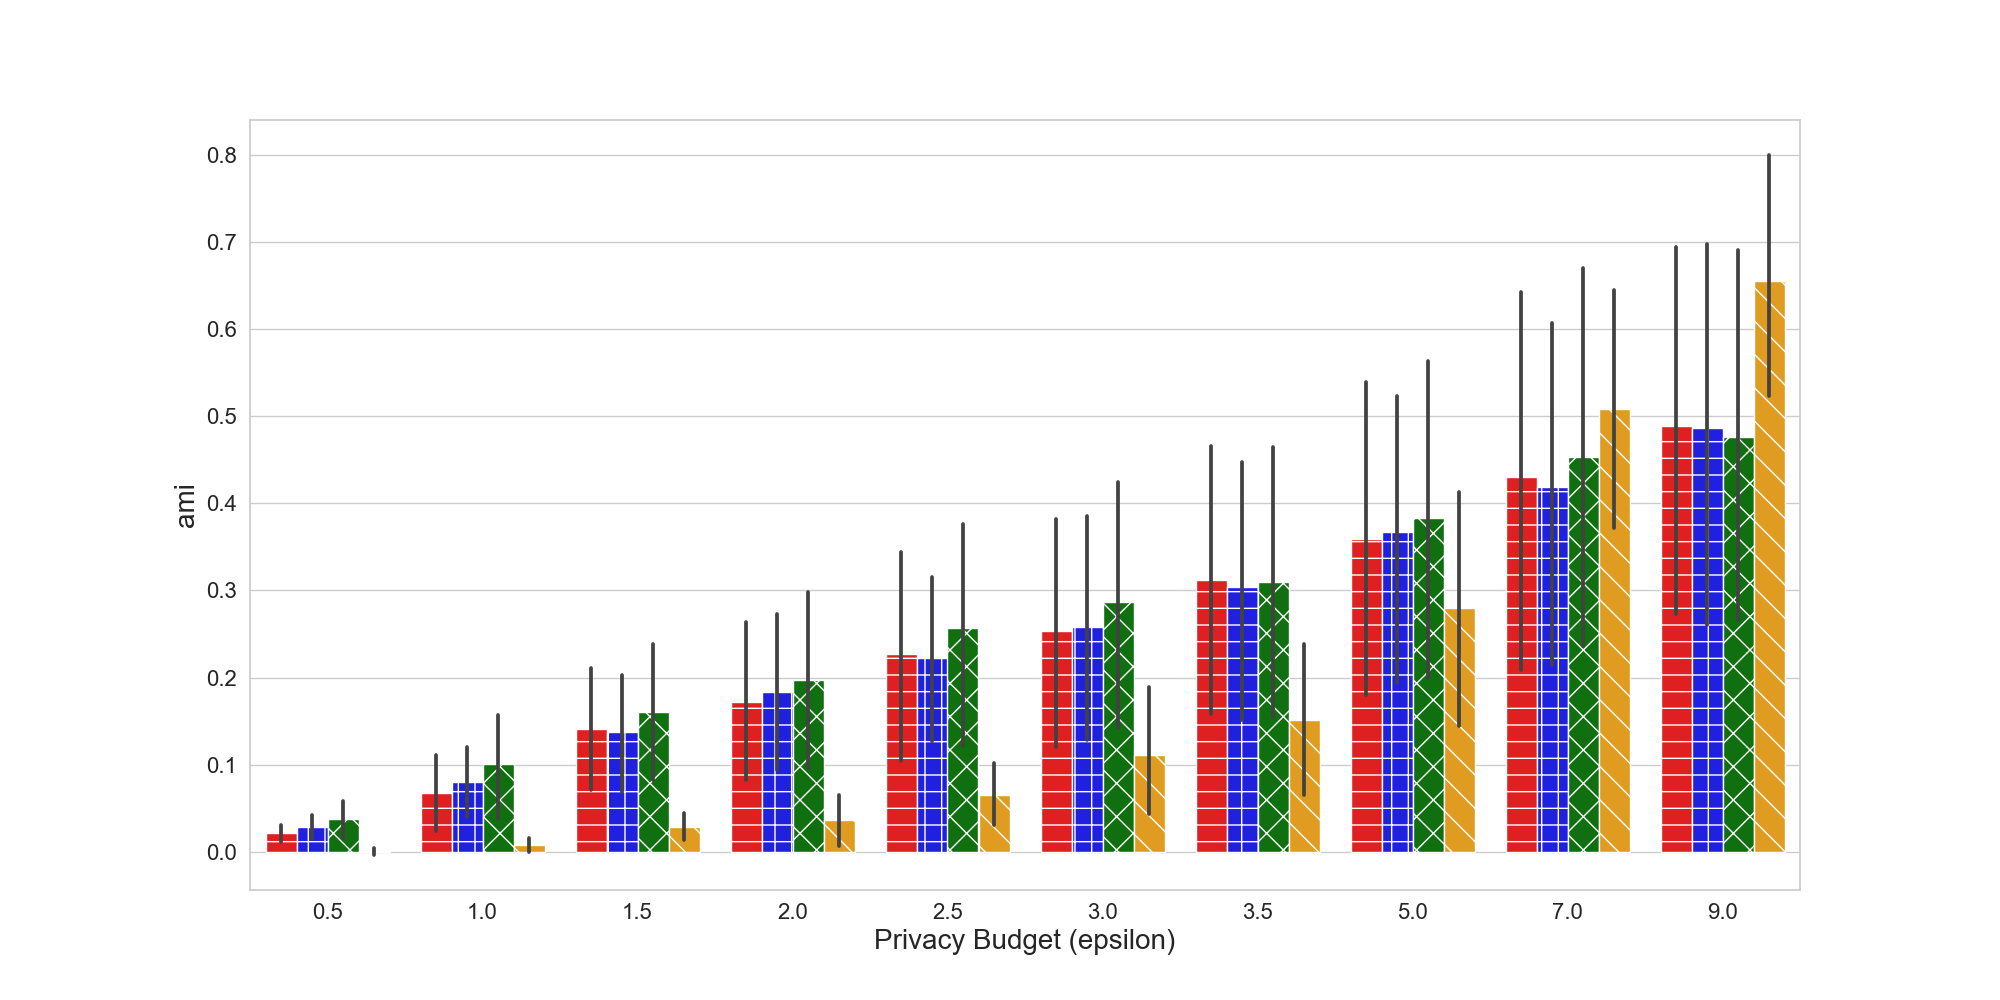
\includegraphics[width=1\textwidth]{Results/nd-laplace/ami_skewed-dataset_comparison.png}
  \end{subfigure}
  \begin{subfigure}{1\textwidth}
    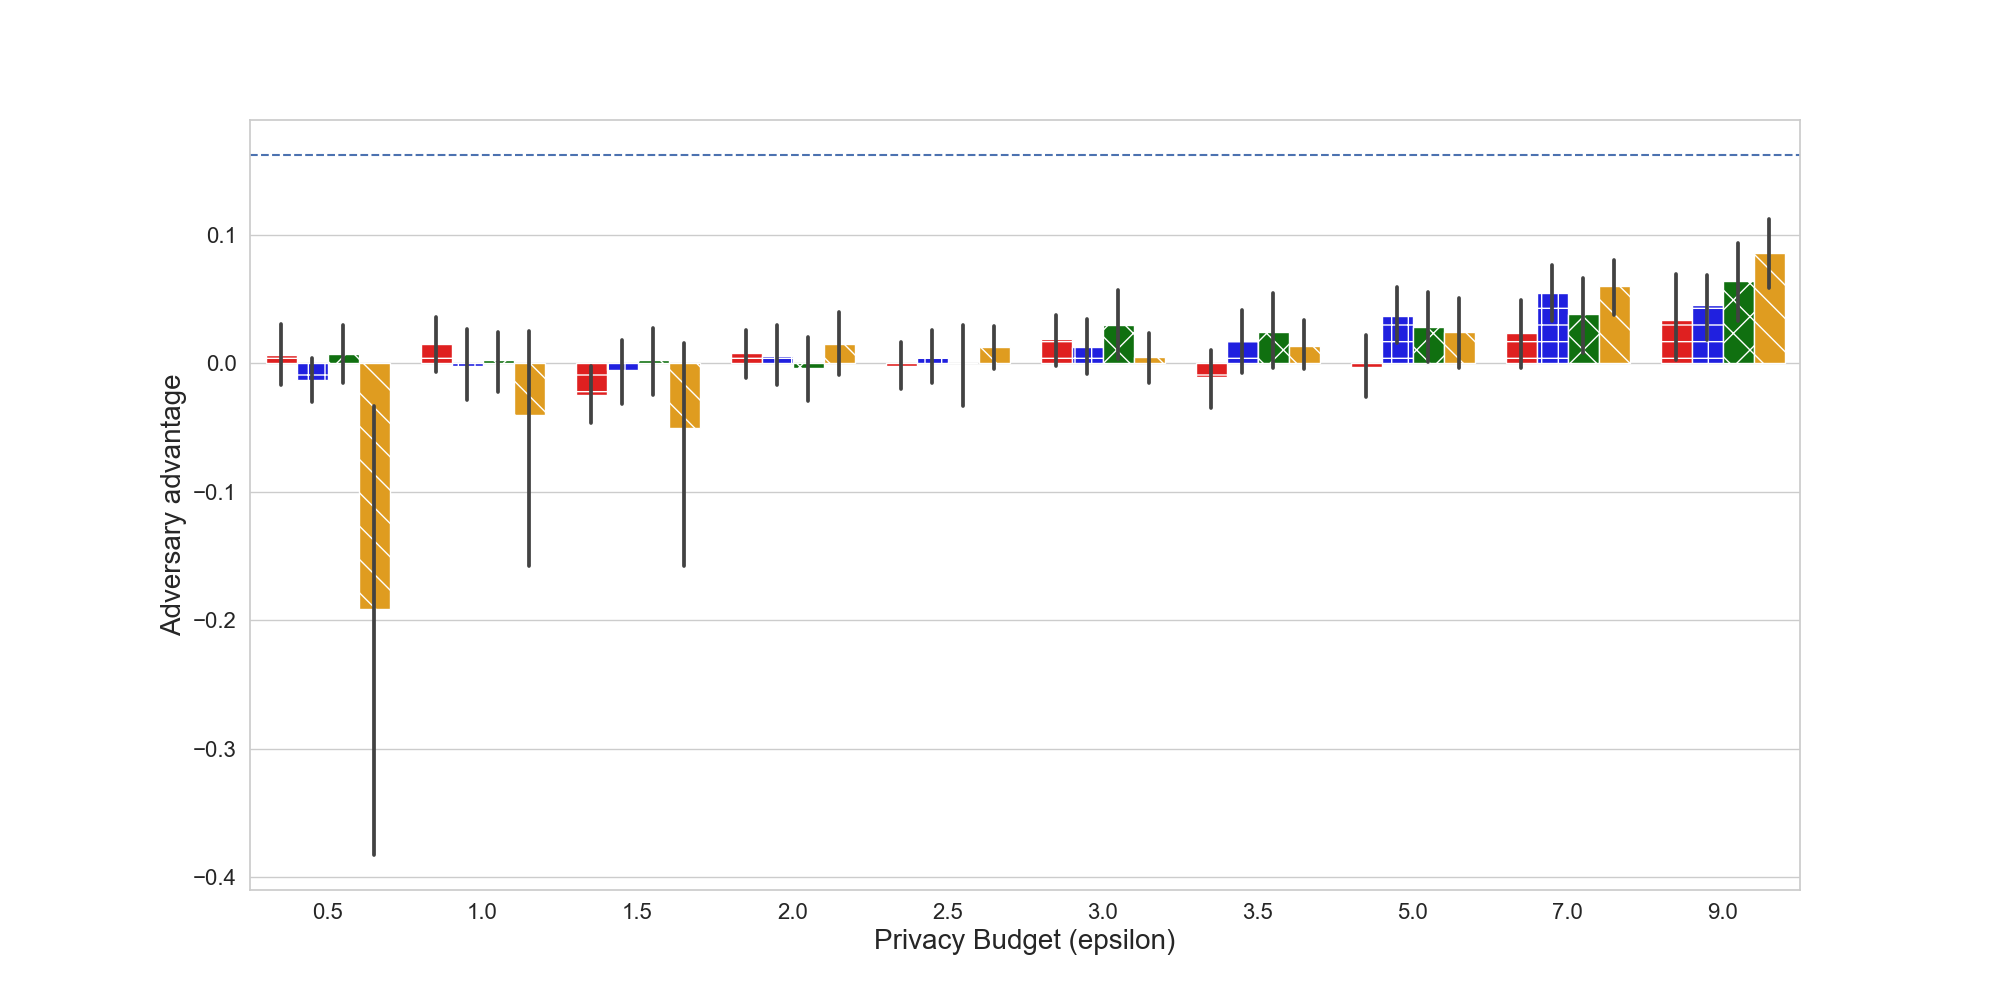
\includegraphics[width=1\textwidth]{Results/nd-laplace/attack_adv_skewed-dataset_comparison.png}
  \end{subfigure}
  \caption{Average AMI (top) and Adversary Advantage (bottom) comparison for each mechanism for skewed-dataset (3 dimensions).}
  \label{fig:utility_skewed-dataset_comparison_nd_plot}
\end{figure}
The nD-Laplace mechanism consistently exhibits a nearly uniform \gls{ami} across all privacy budgets. In contrast, the Piecewise mechanism generally registers lower scores for most privacy budgets, with an exception at privacy budget 9 where it surpasses the former. This pattern aligns with our observations from the cluster utility and heatmap analyses. The enhanced performance of the Piecewise mechanism at higher privacy budgets can be attributed to its ability to retain the shape of the data, as evidenced in the 2-dimensional line-dataset and seeds-dataset. Mirroring trends from other plots, the Piecewise mechanism demonstrates superior privacy levels at lower privacy budgets. Yet, when considering higher privacy budgets, the variants of the nD-Laplace mechanism prove to be more effective.
\newpage



\begin{figure}[H]
  \centering
  \begin{subfigure}{0.30\textwidth}
    \includegraphics[width=\textwidth]{Results/kd-laplace/ami_bar_comparison_legend.png}
  \end{subfigure}
  \begin{subfigure}{1\textwidth}
    \includegraphics[width=1\textwidth]{Results/nd-laplace/ami_line-dataset_comparison.png}
  \end{subfigure}
  \begin{subfigure}{1\textwidth}
    \includegraphics[width=1\textwidth]{Results/nd-laplace/attack_adv_line-dataset_comparison.png}
  \end{subfigure}
  \caption{Average AMI (top) and Adversary Advantage (bottom) comparison for each mechanism for line-dataset (3 dimensions).}
  \label{fig:utility_line-dataset_comparison_nd_plot}
\end{figure}
The nD-Laplace mechanism exhibits suboptimal performance in terms of \gls{ami}. This can be attributed to its uniform distribution, which is not well-suited for datasets with a line-shaped structure, as illustrated in Figure \ref{fig:validation-Line-dataset_comparison_2d-laplace}. In contrast, the Piecewise mechanism more effectively retains the original shape, though it registers an average \gls{ami} of 0.6 for a privacy budget of 9. Notably, the majority of the values surpass the baseline in terms of privacy. Furthermore, it is observed that for an epsilon value of 0.5, a significant number of mechanisms exhibit a negative membership advantage.